
	\begin{figure}
		\centering
		\subfloat[SHREK]{
			\scalebox{.4}{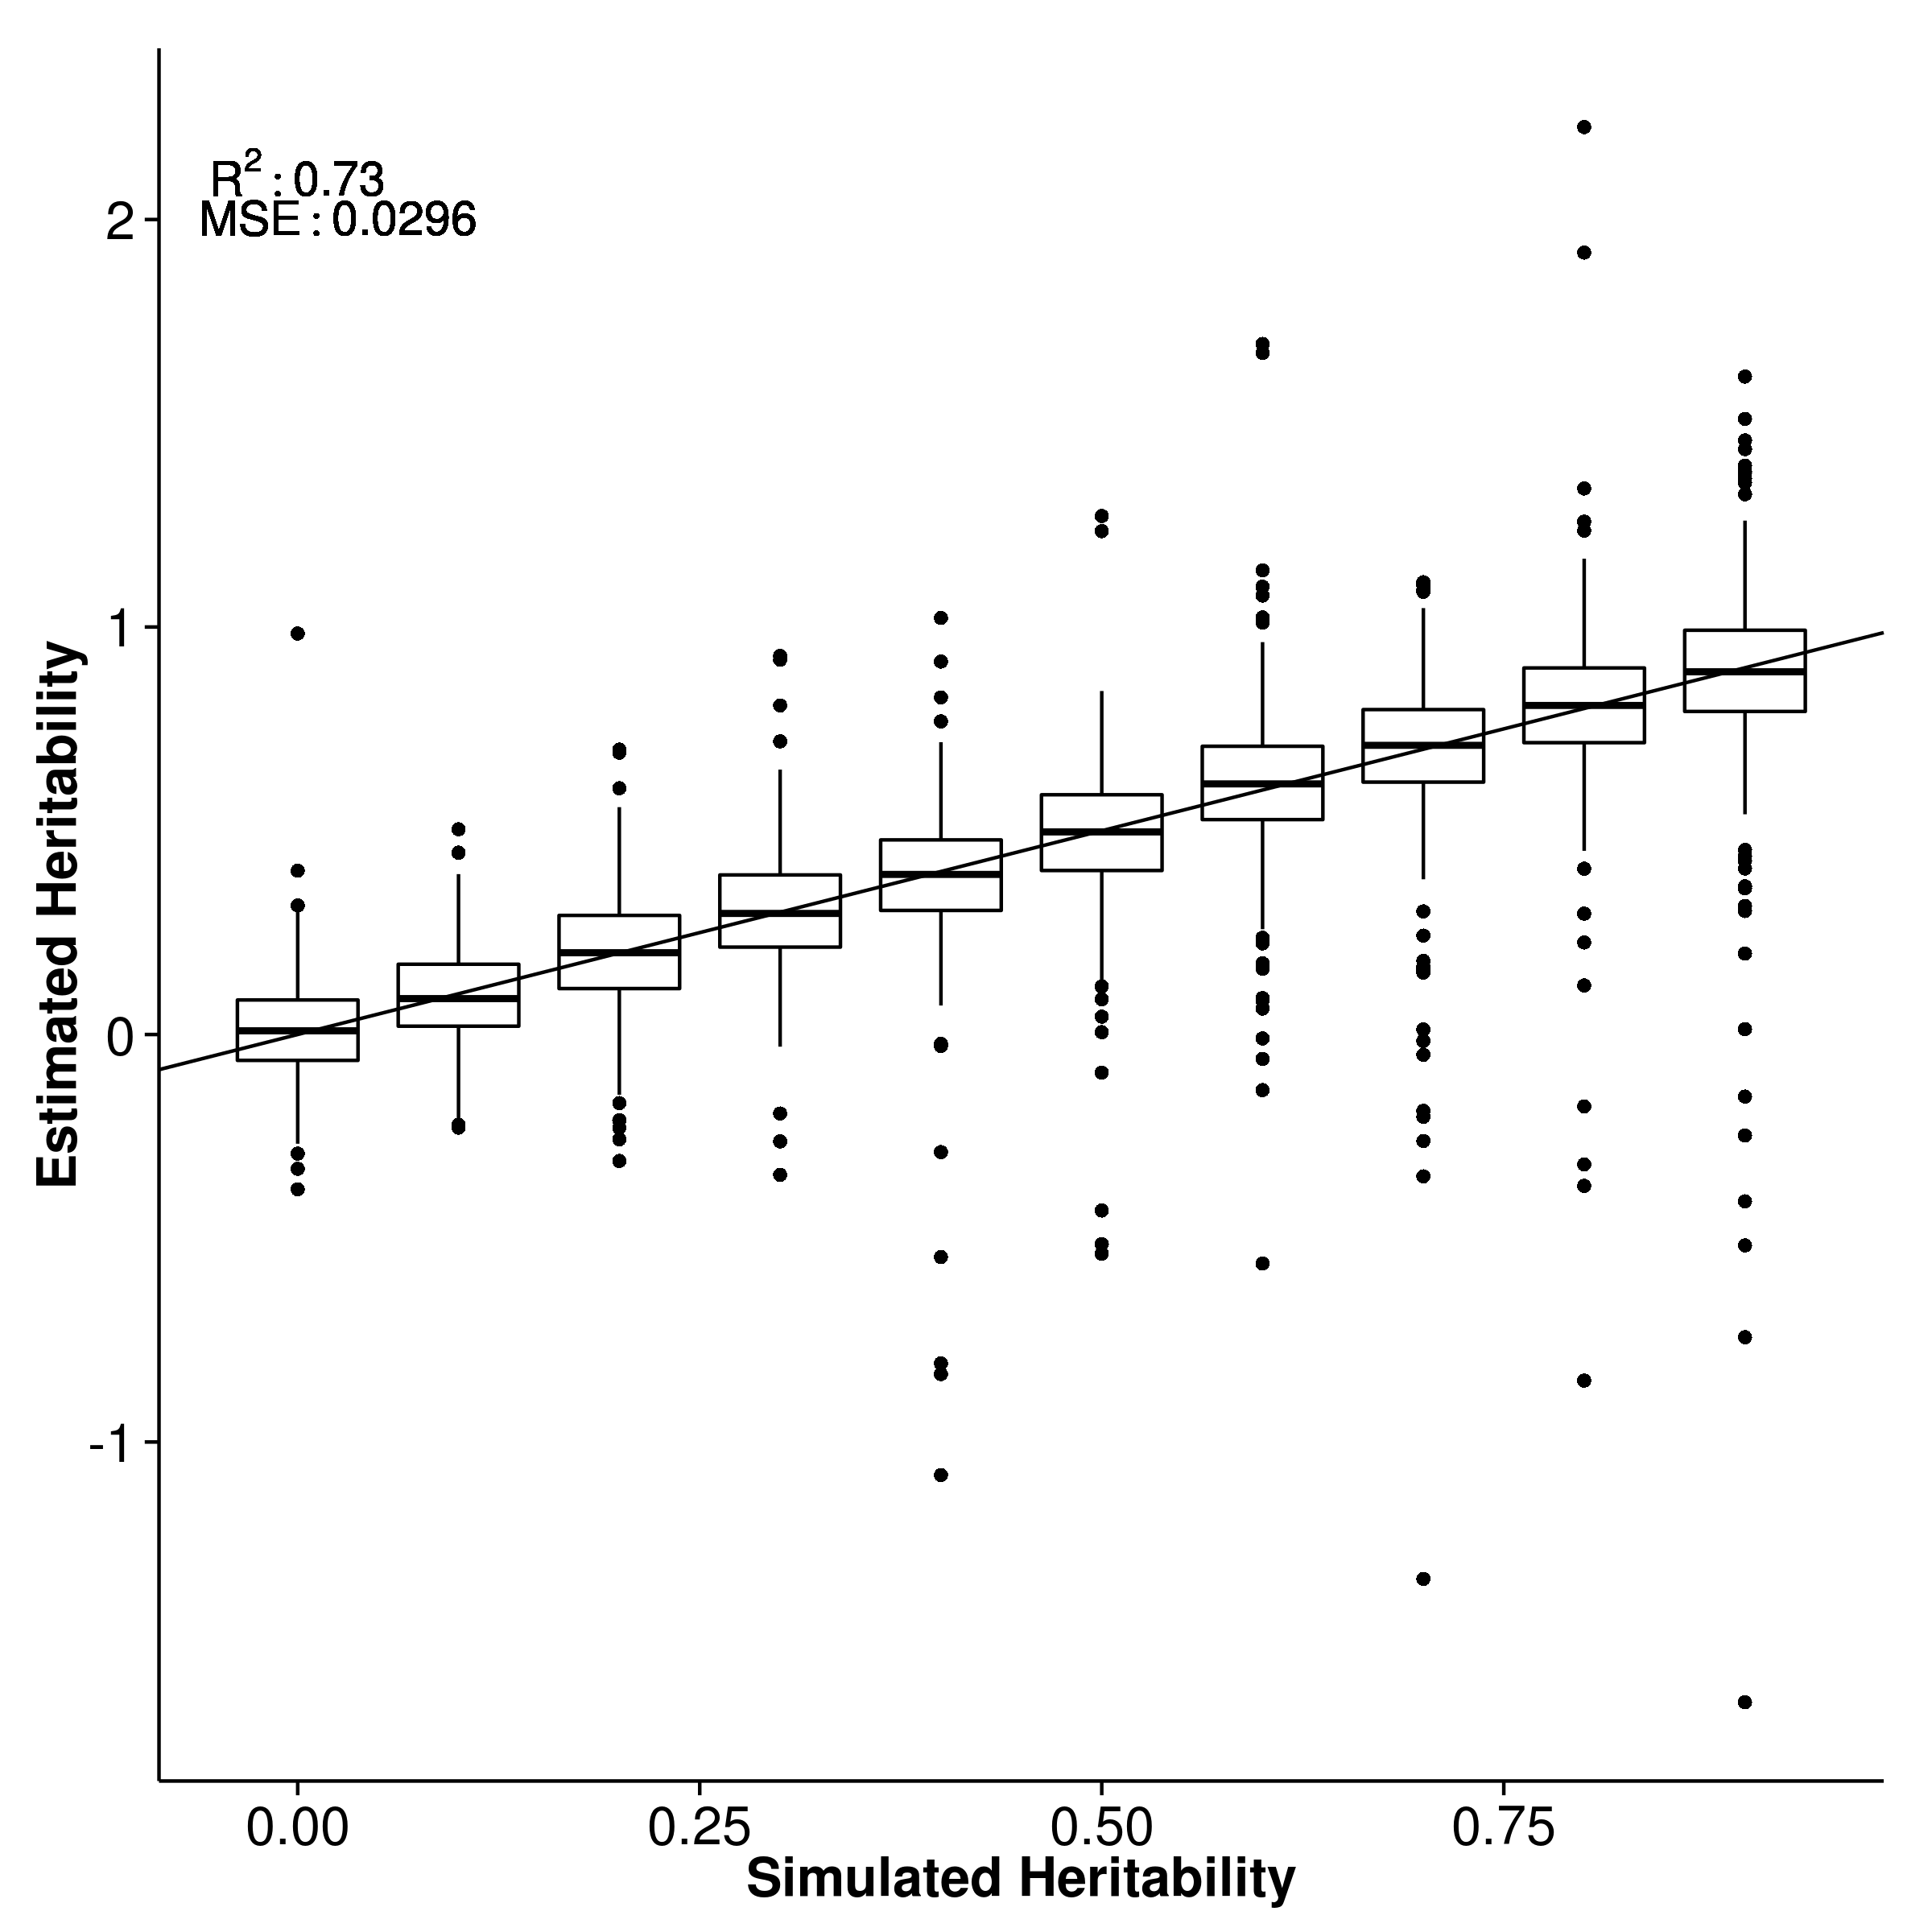
\includegraphics{figure/quantitative/same_effect/10c/shrek_50k_10c_meanH.png}}
			\label{fig:50k10cQtmeanS}
		}
		\subfloat[GCTA]{
			\scalebox{.4}{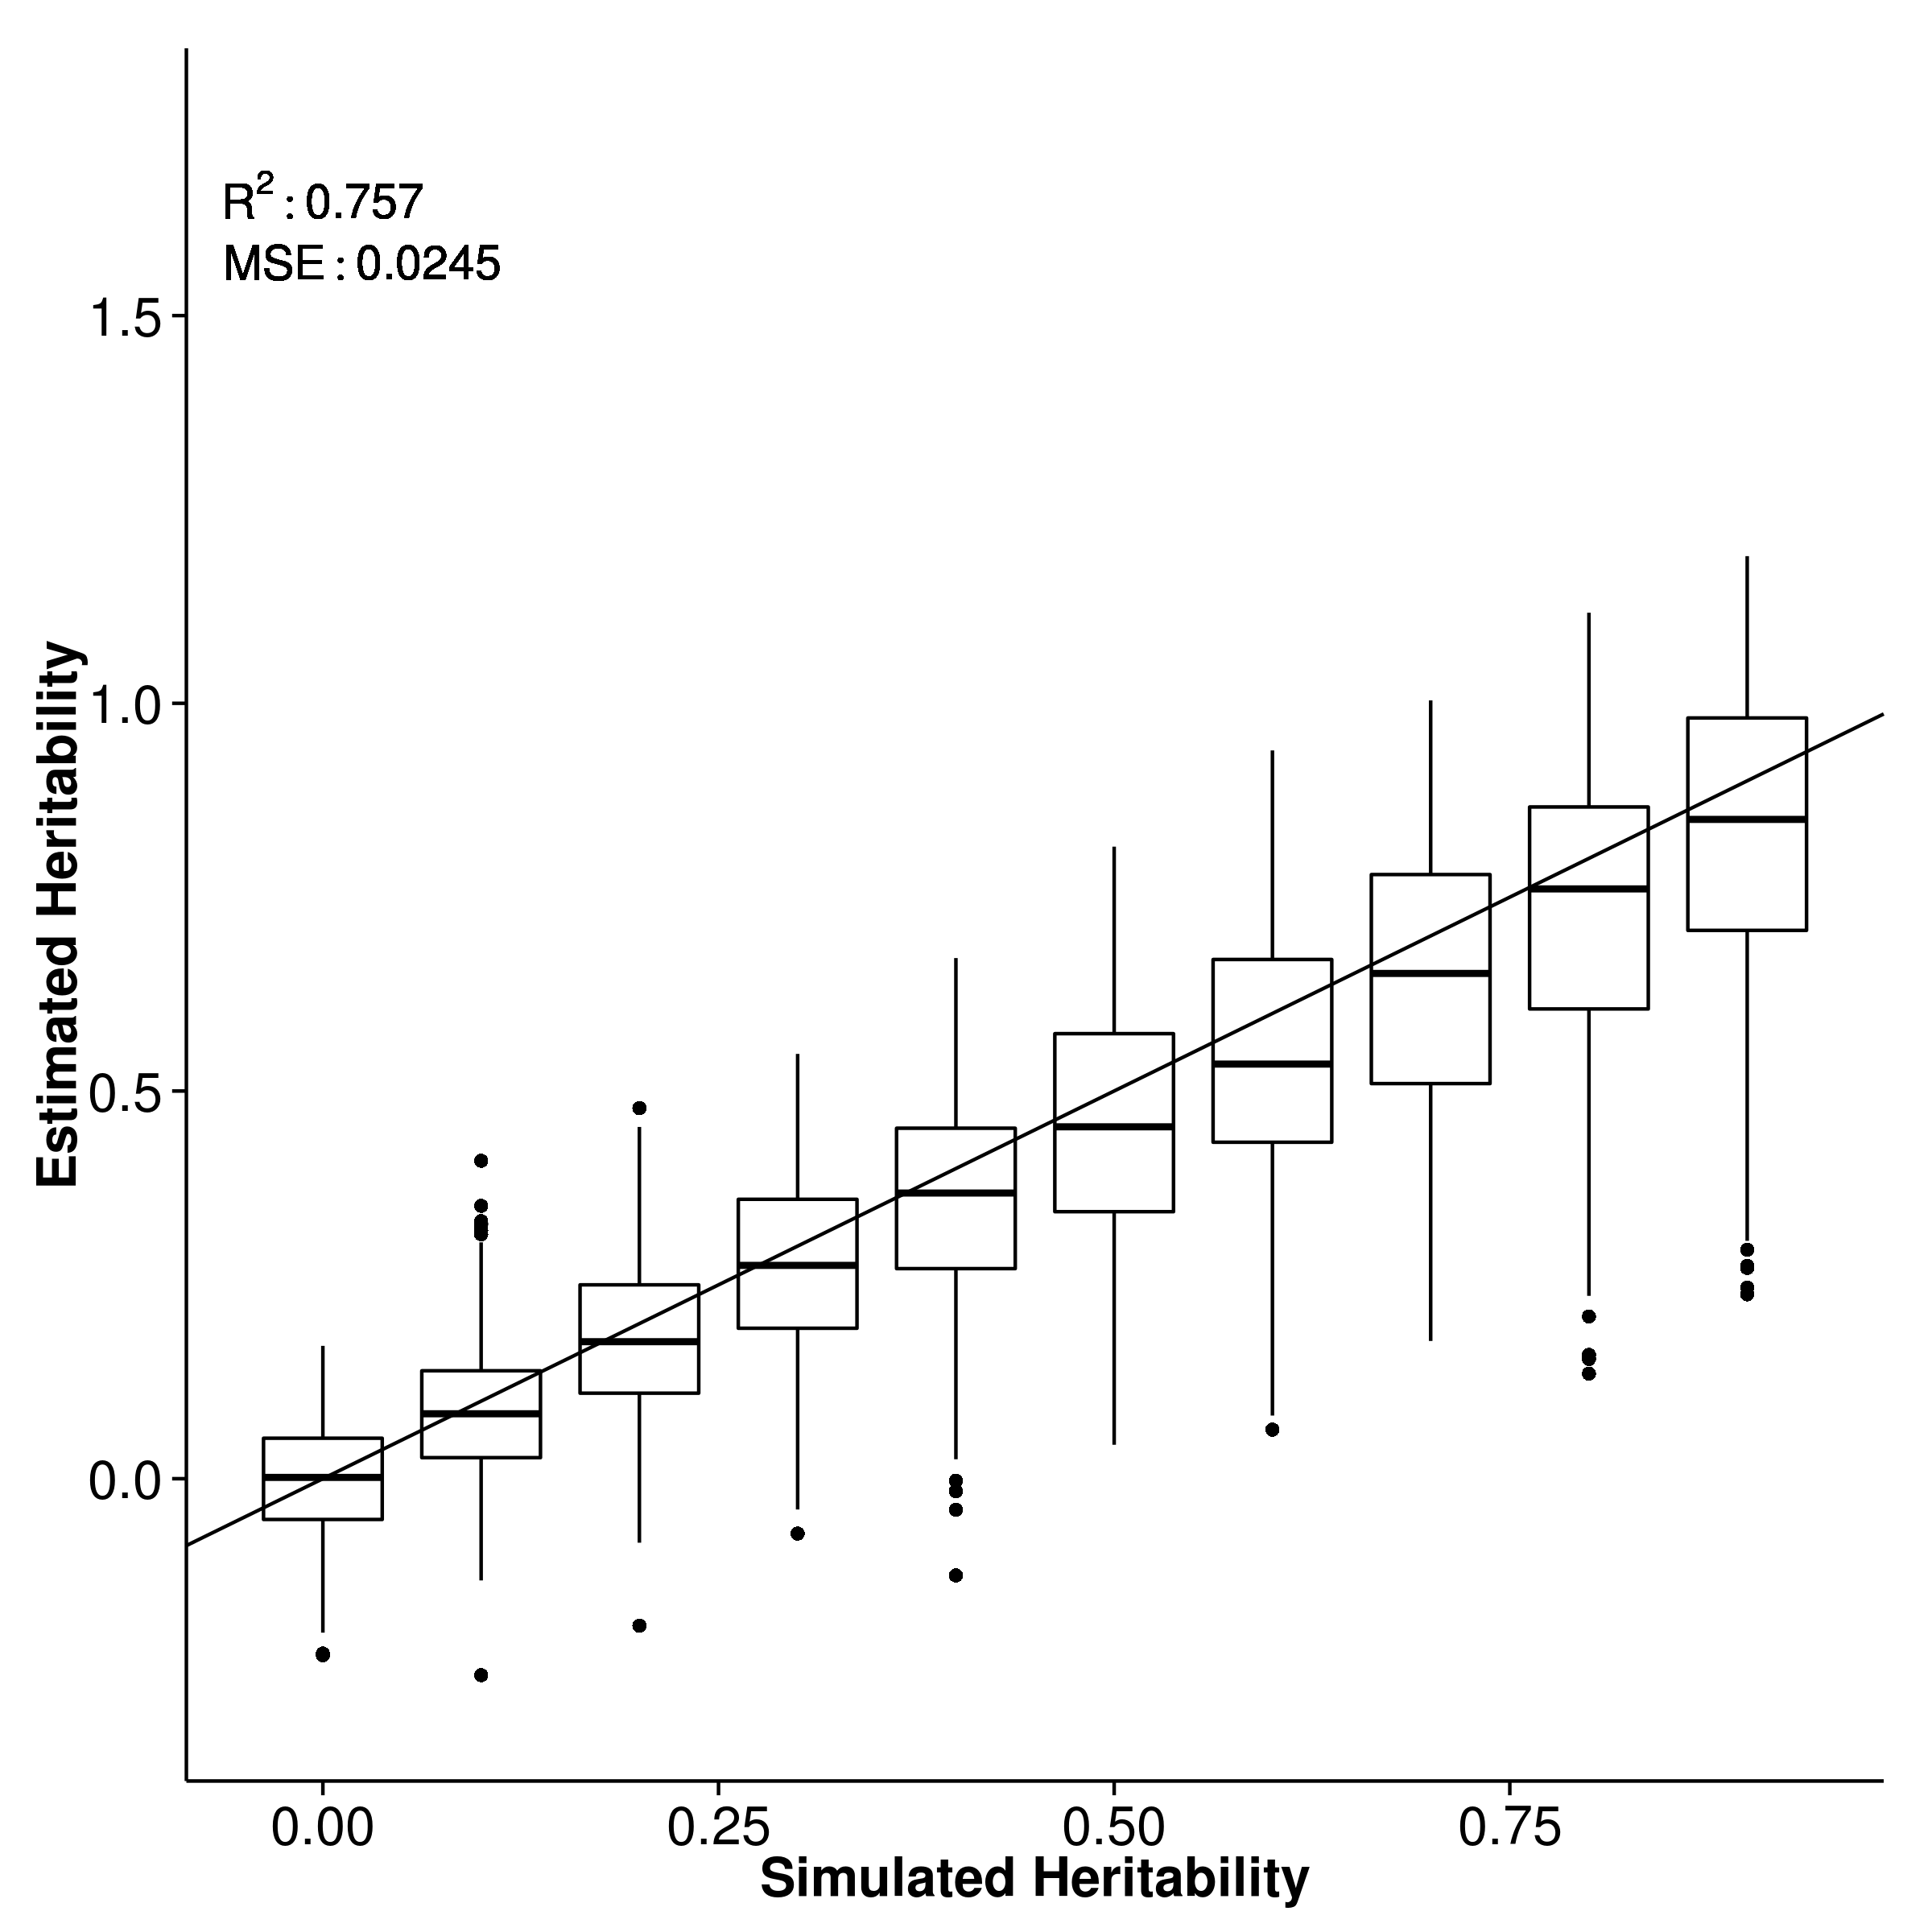
\includegraphics{figure/quantitative/same_effect/10c/gcta_50k_10c_meanH.png}}
			\label{fig:50k10cQtmeanG}
		}\\
		\subfloat[LDSC with fix intercept]{
			\scalebox{.4}{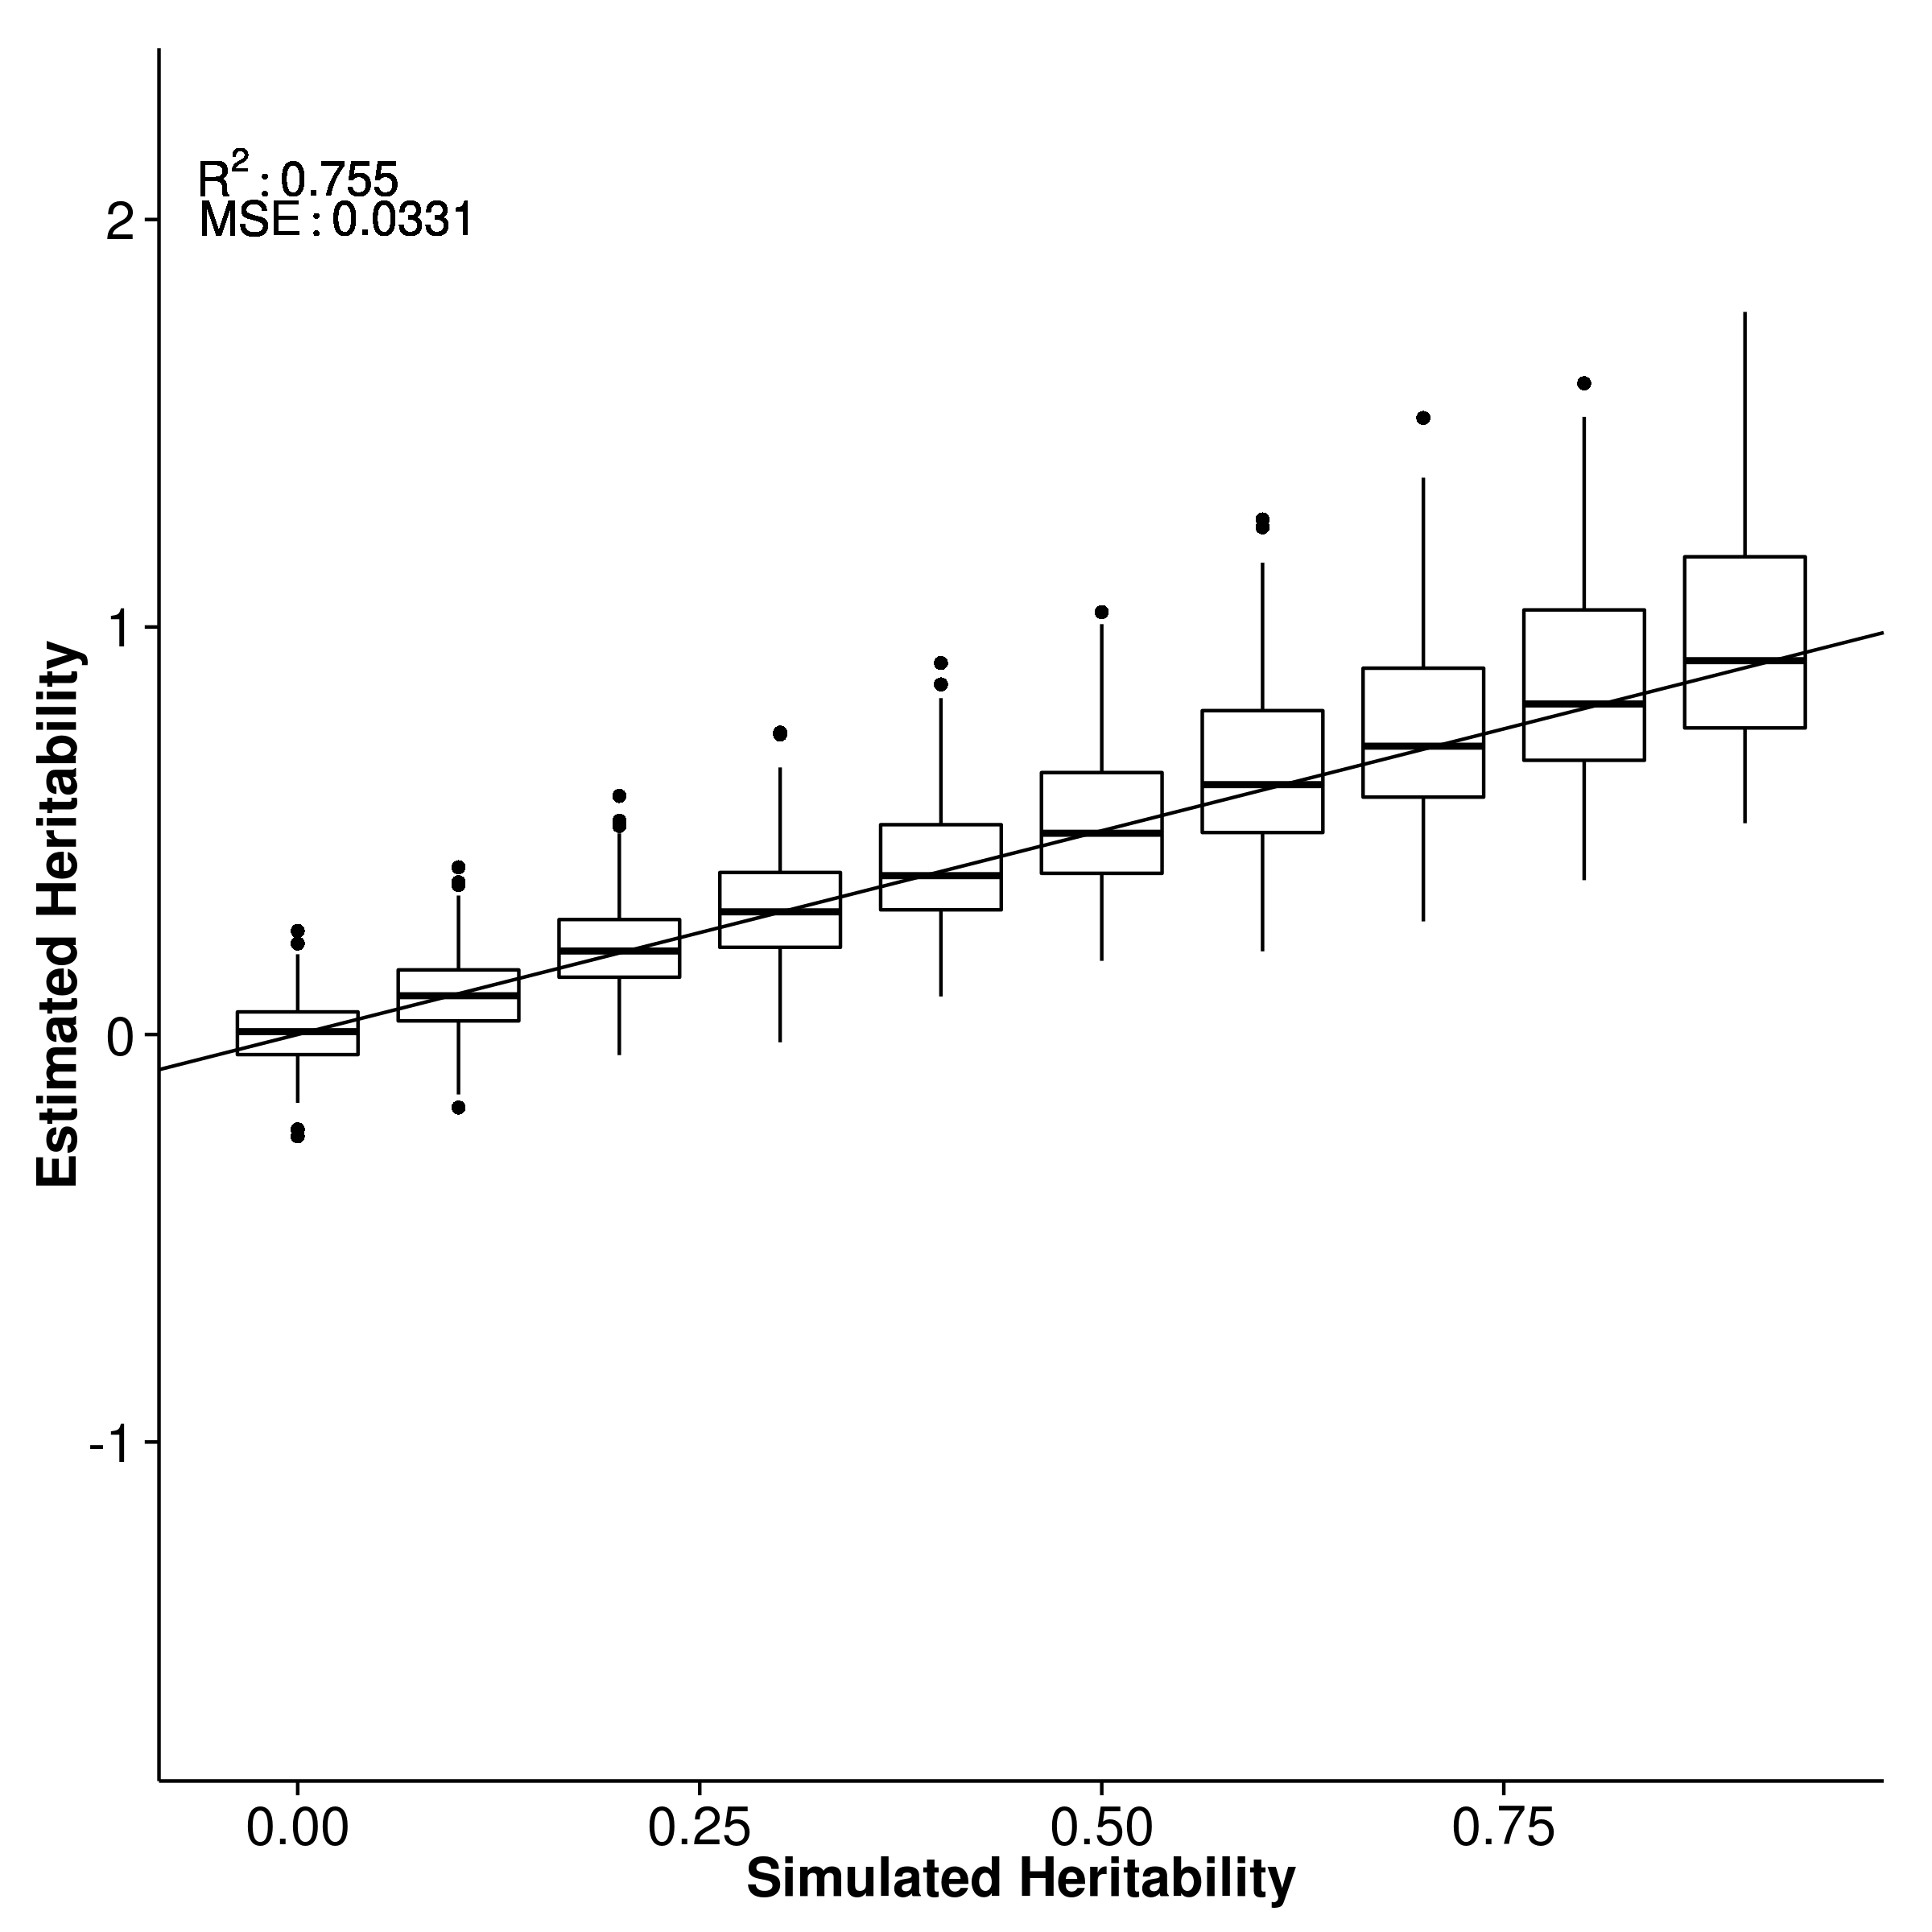
\includegraphics{figure/quantitative/same_effect/10c/ldsc_50k_10c_meanH.png}}
			\label{fig:50k10cQtmeanL}
		}
		\subfloat[LDSC with intercept estimation]{
			\scalebox{.4}{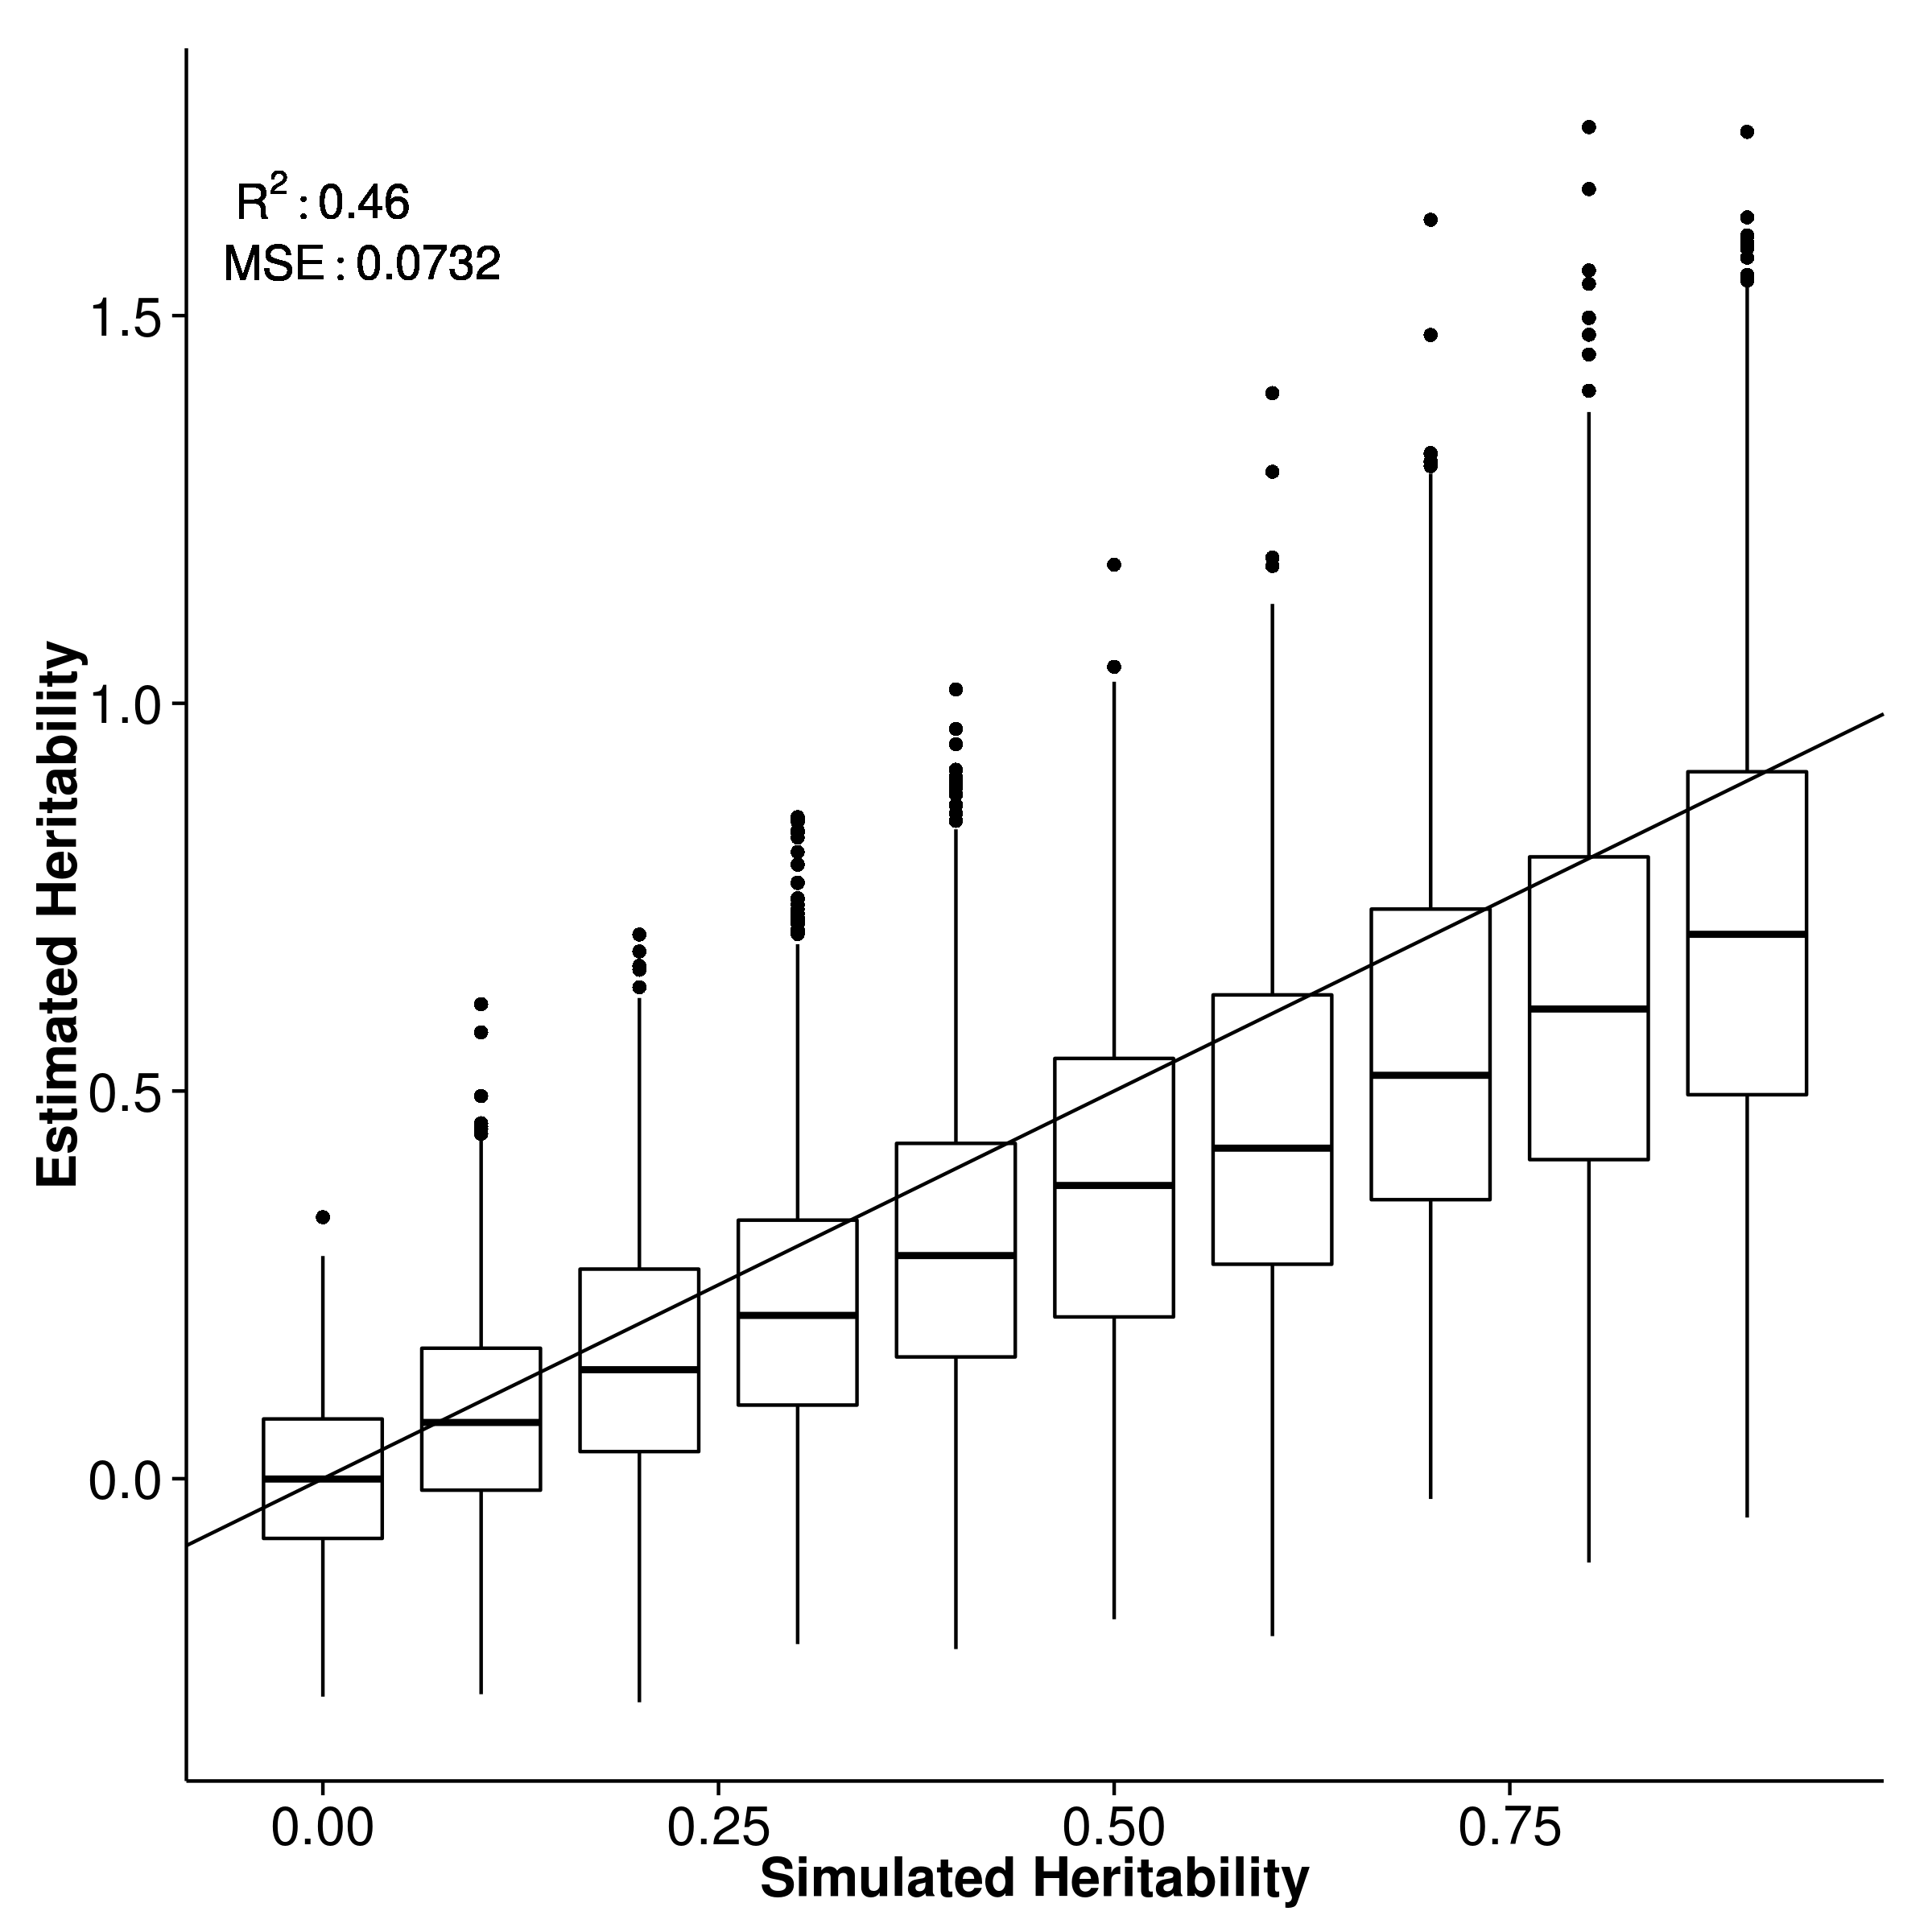
\includegraphics{figure/quantitative/same_effect/10c/ldscIn_50k_10c_meanH.png}}
			\label{fig:50k10cQtmeanI}
		}
		\caption[Simulation of Quantitative Traits with 50k \glsentryshortpl{SNP} and 10 causal variants of same effect size]
		{Simulation of Quantitative Traits with 50k \glsentryshortpl{SNP} and 10 causal variants with same effect size.
			It was observed that of all the tools, \gls{shrek} performed best in such scenario} 
		\label{fig:50k10cQtMean}
	\end{figure}
	\begin{figure}
		\centering
		\subfloat[SHREK]{
			\scalebox{.4}{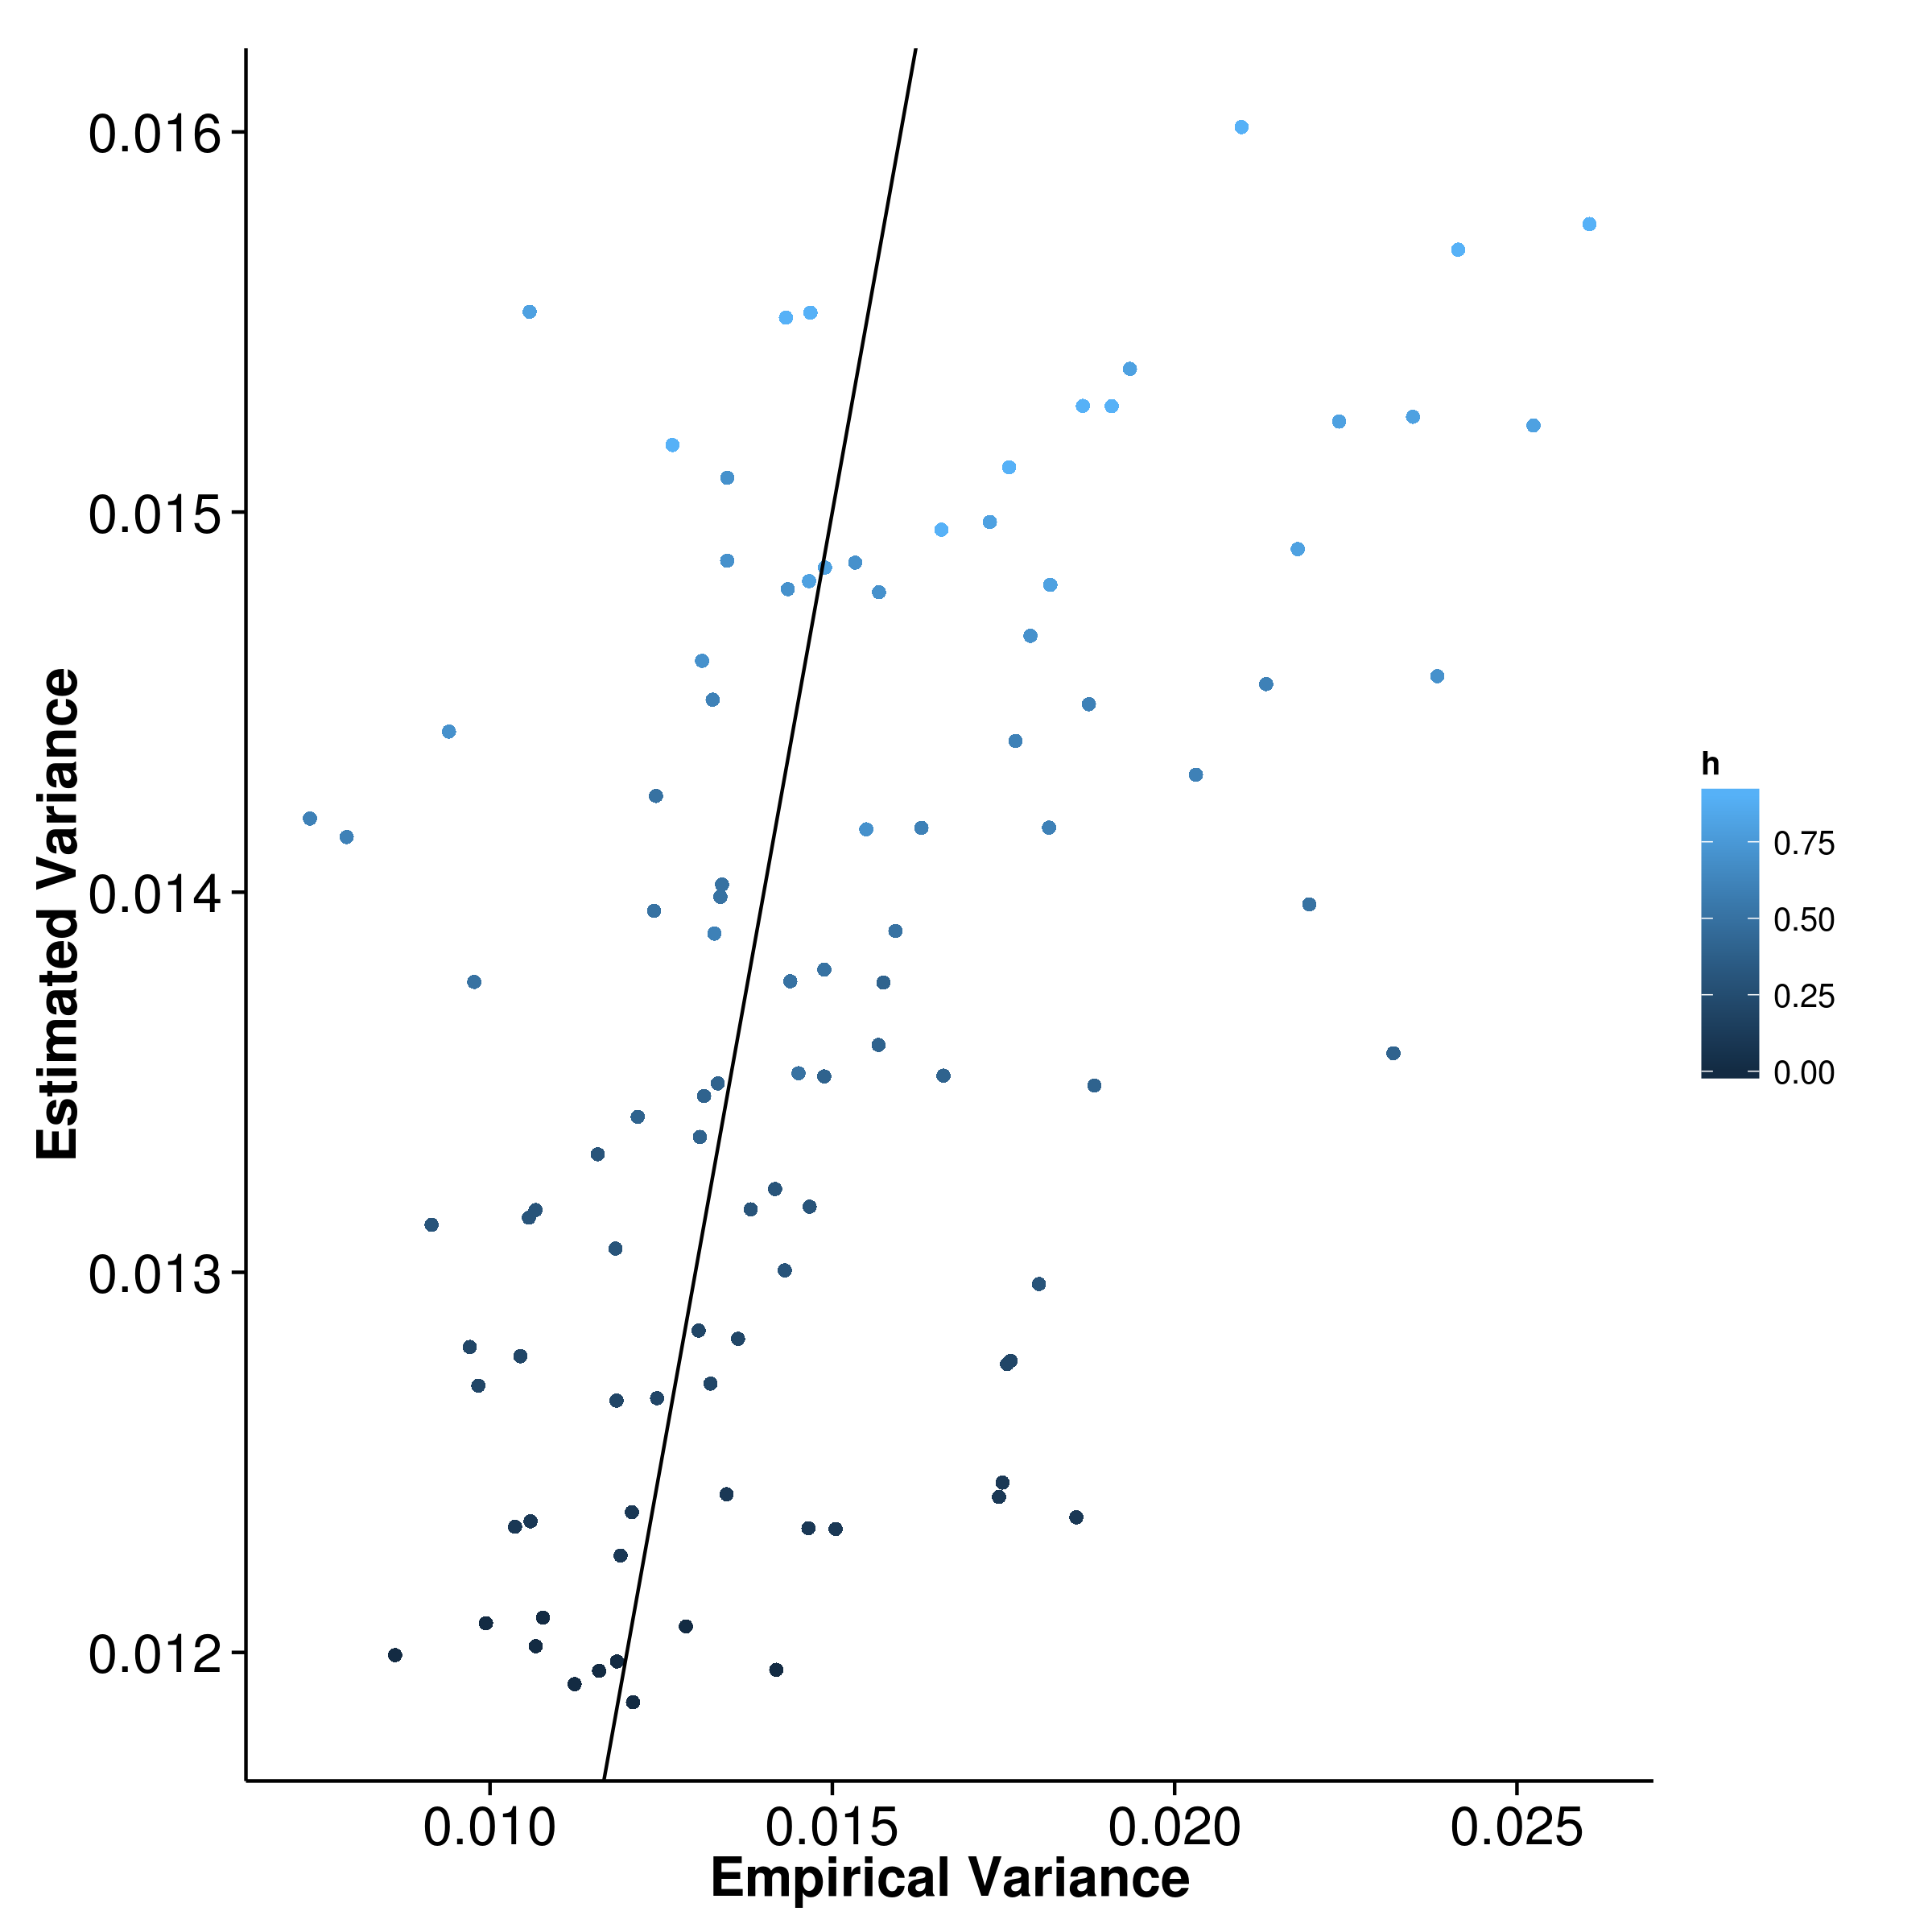
\includegraphics{figure/quantitative/same_effect/10c/shrek_50k_10c_varH.png}}
			\label{fig:50k10cQtvarS}
		}
		\subfloat[GCTA]{
			\scalebox{.4}{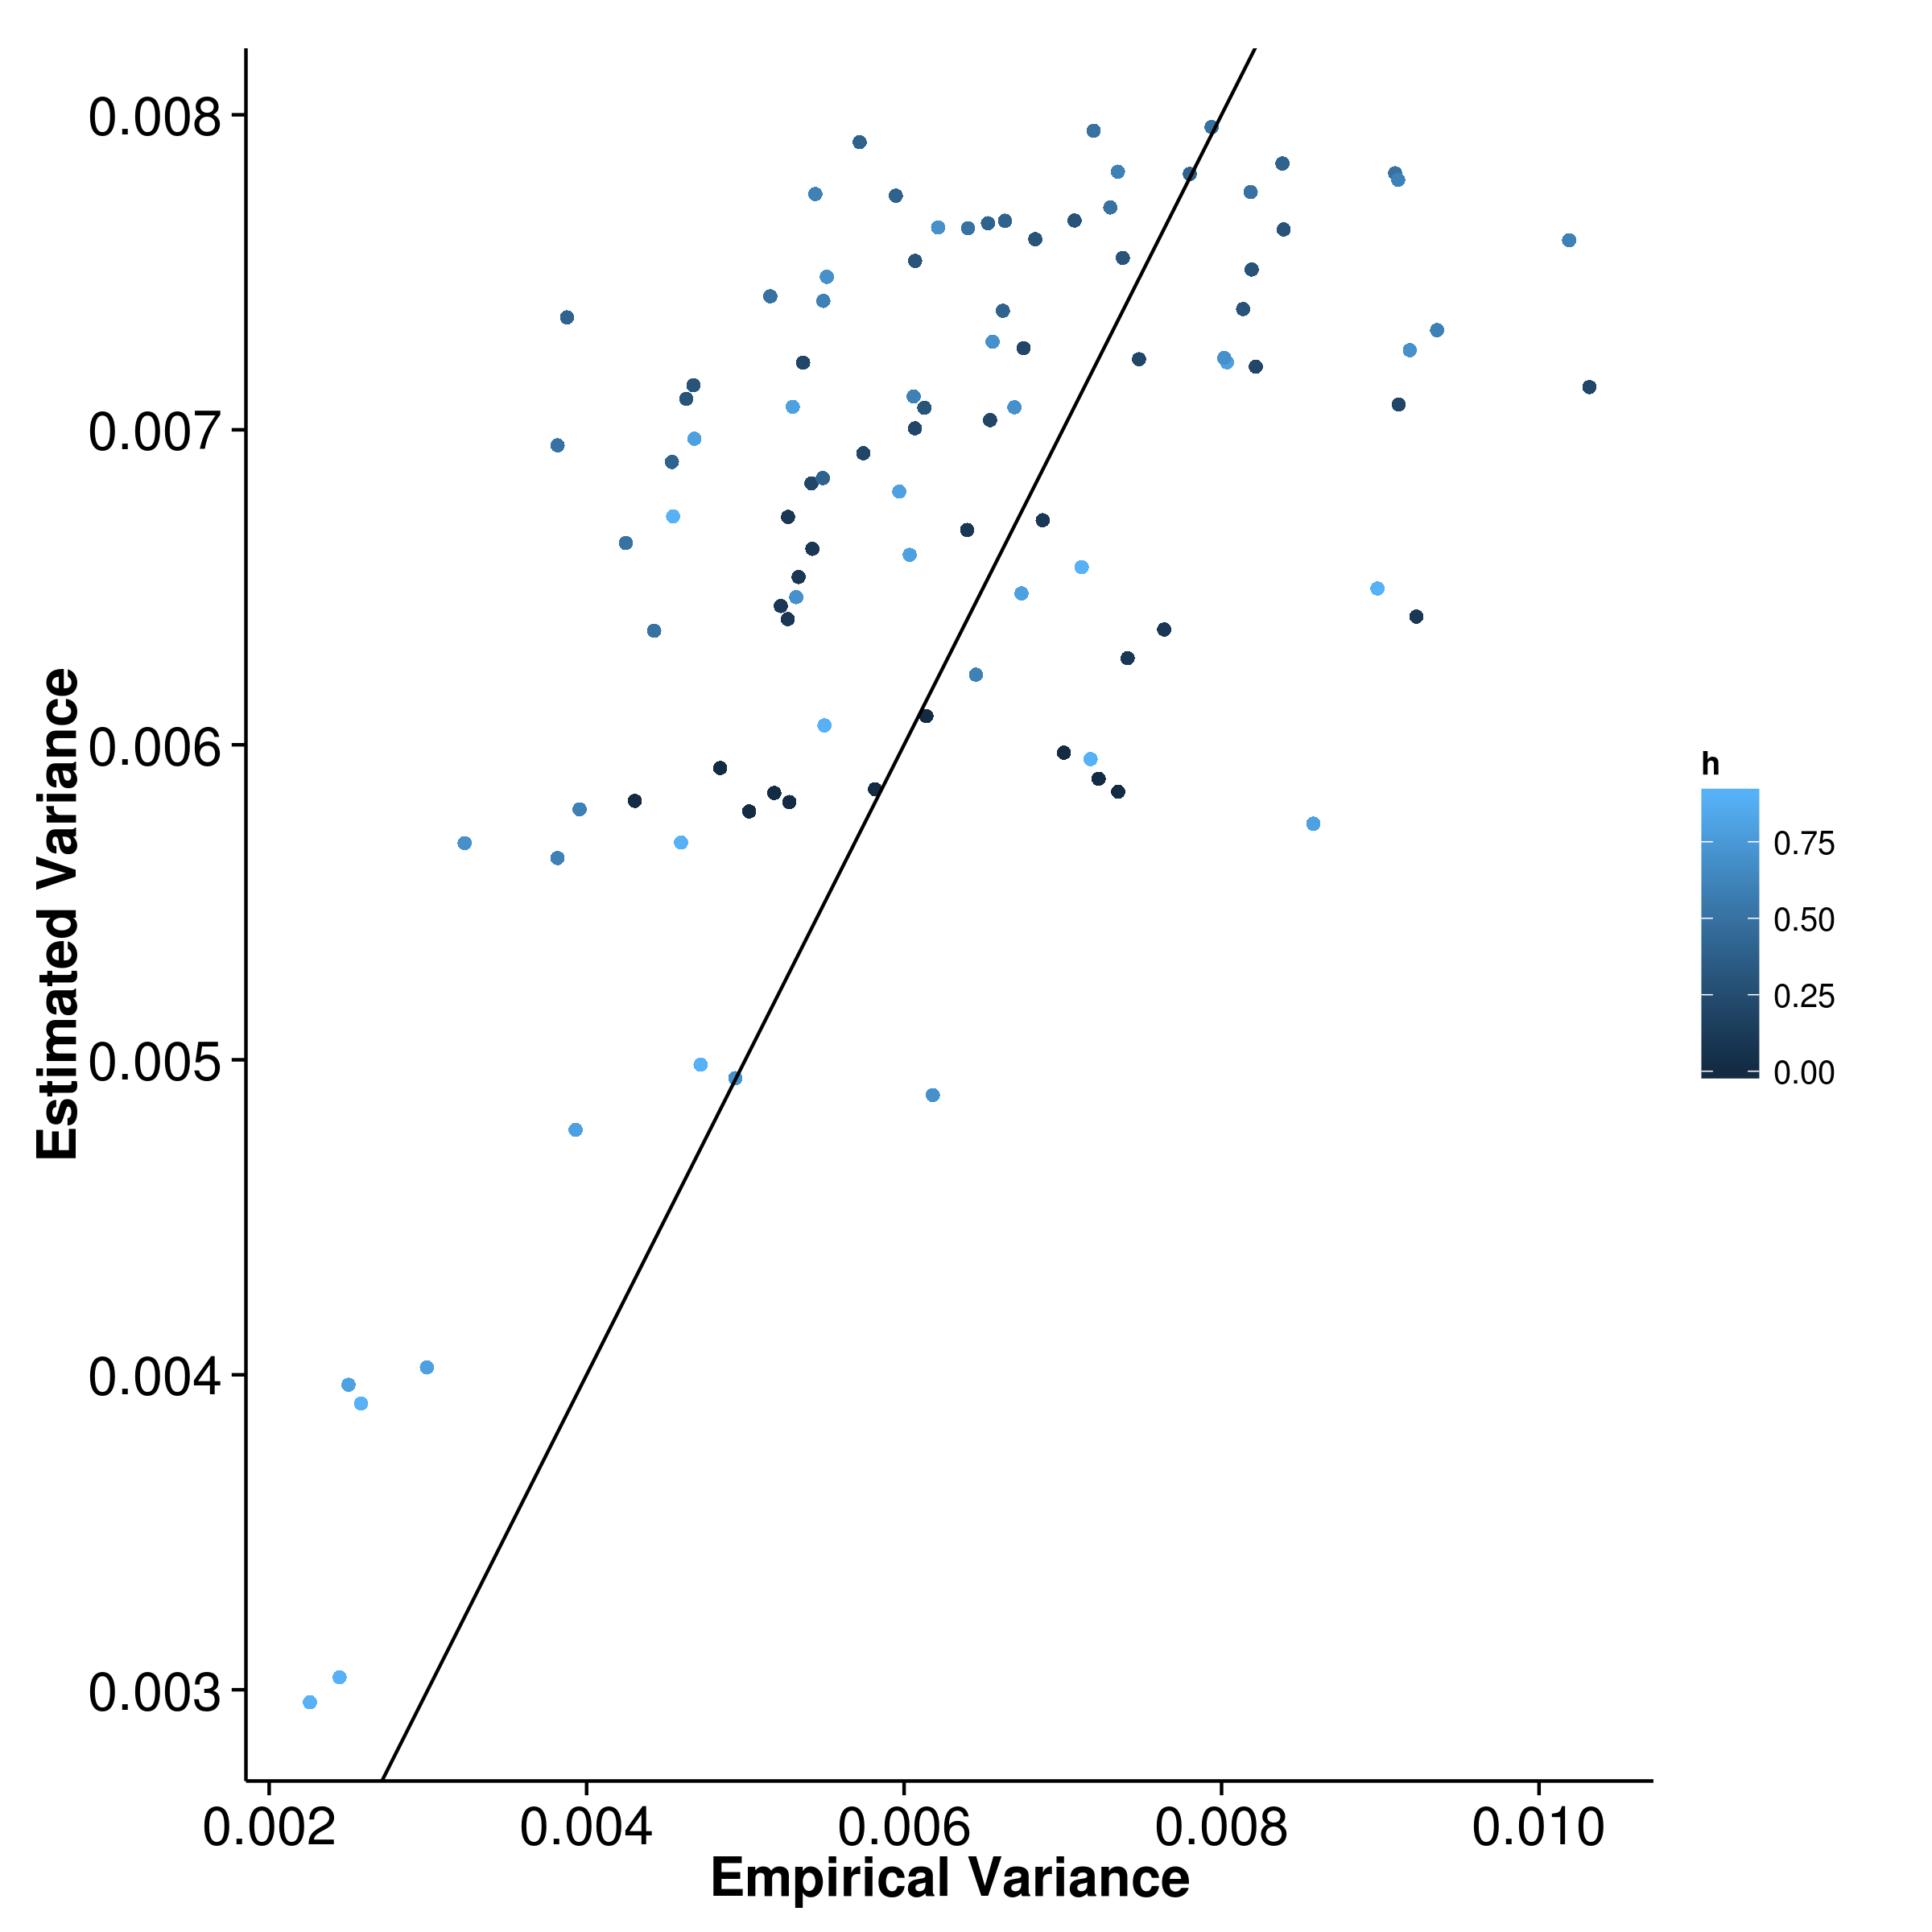
\includegraphics{figure/quantitative/same_effect/10c/gcta_50k_10c_varH.png}}
			\label{fig:50k10cQtvarG}
		}\\
		\subfloat[LDSC with fix intercept]{
			\scalebox{.4}{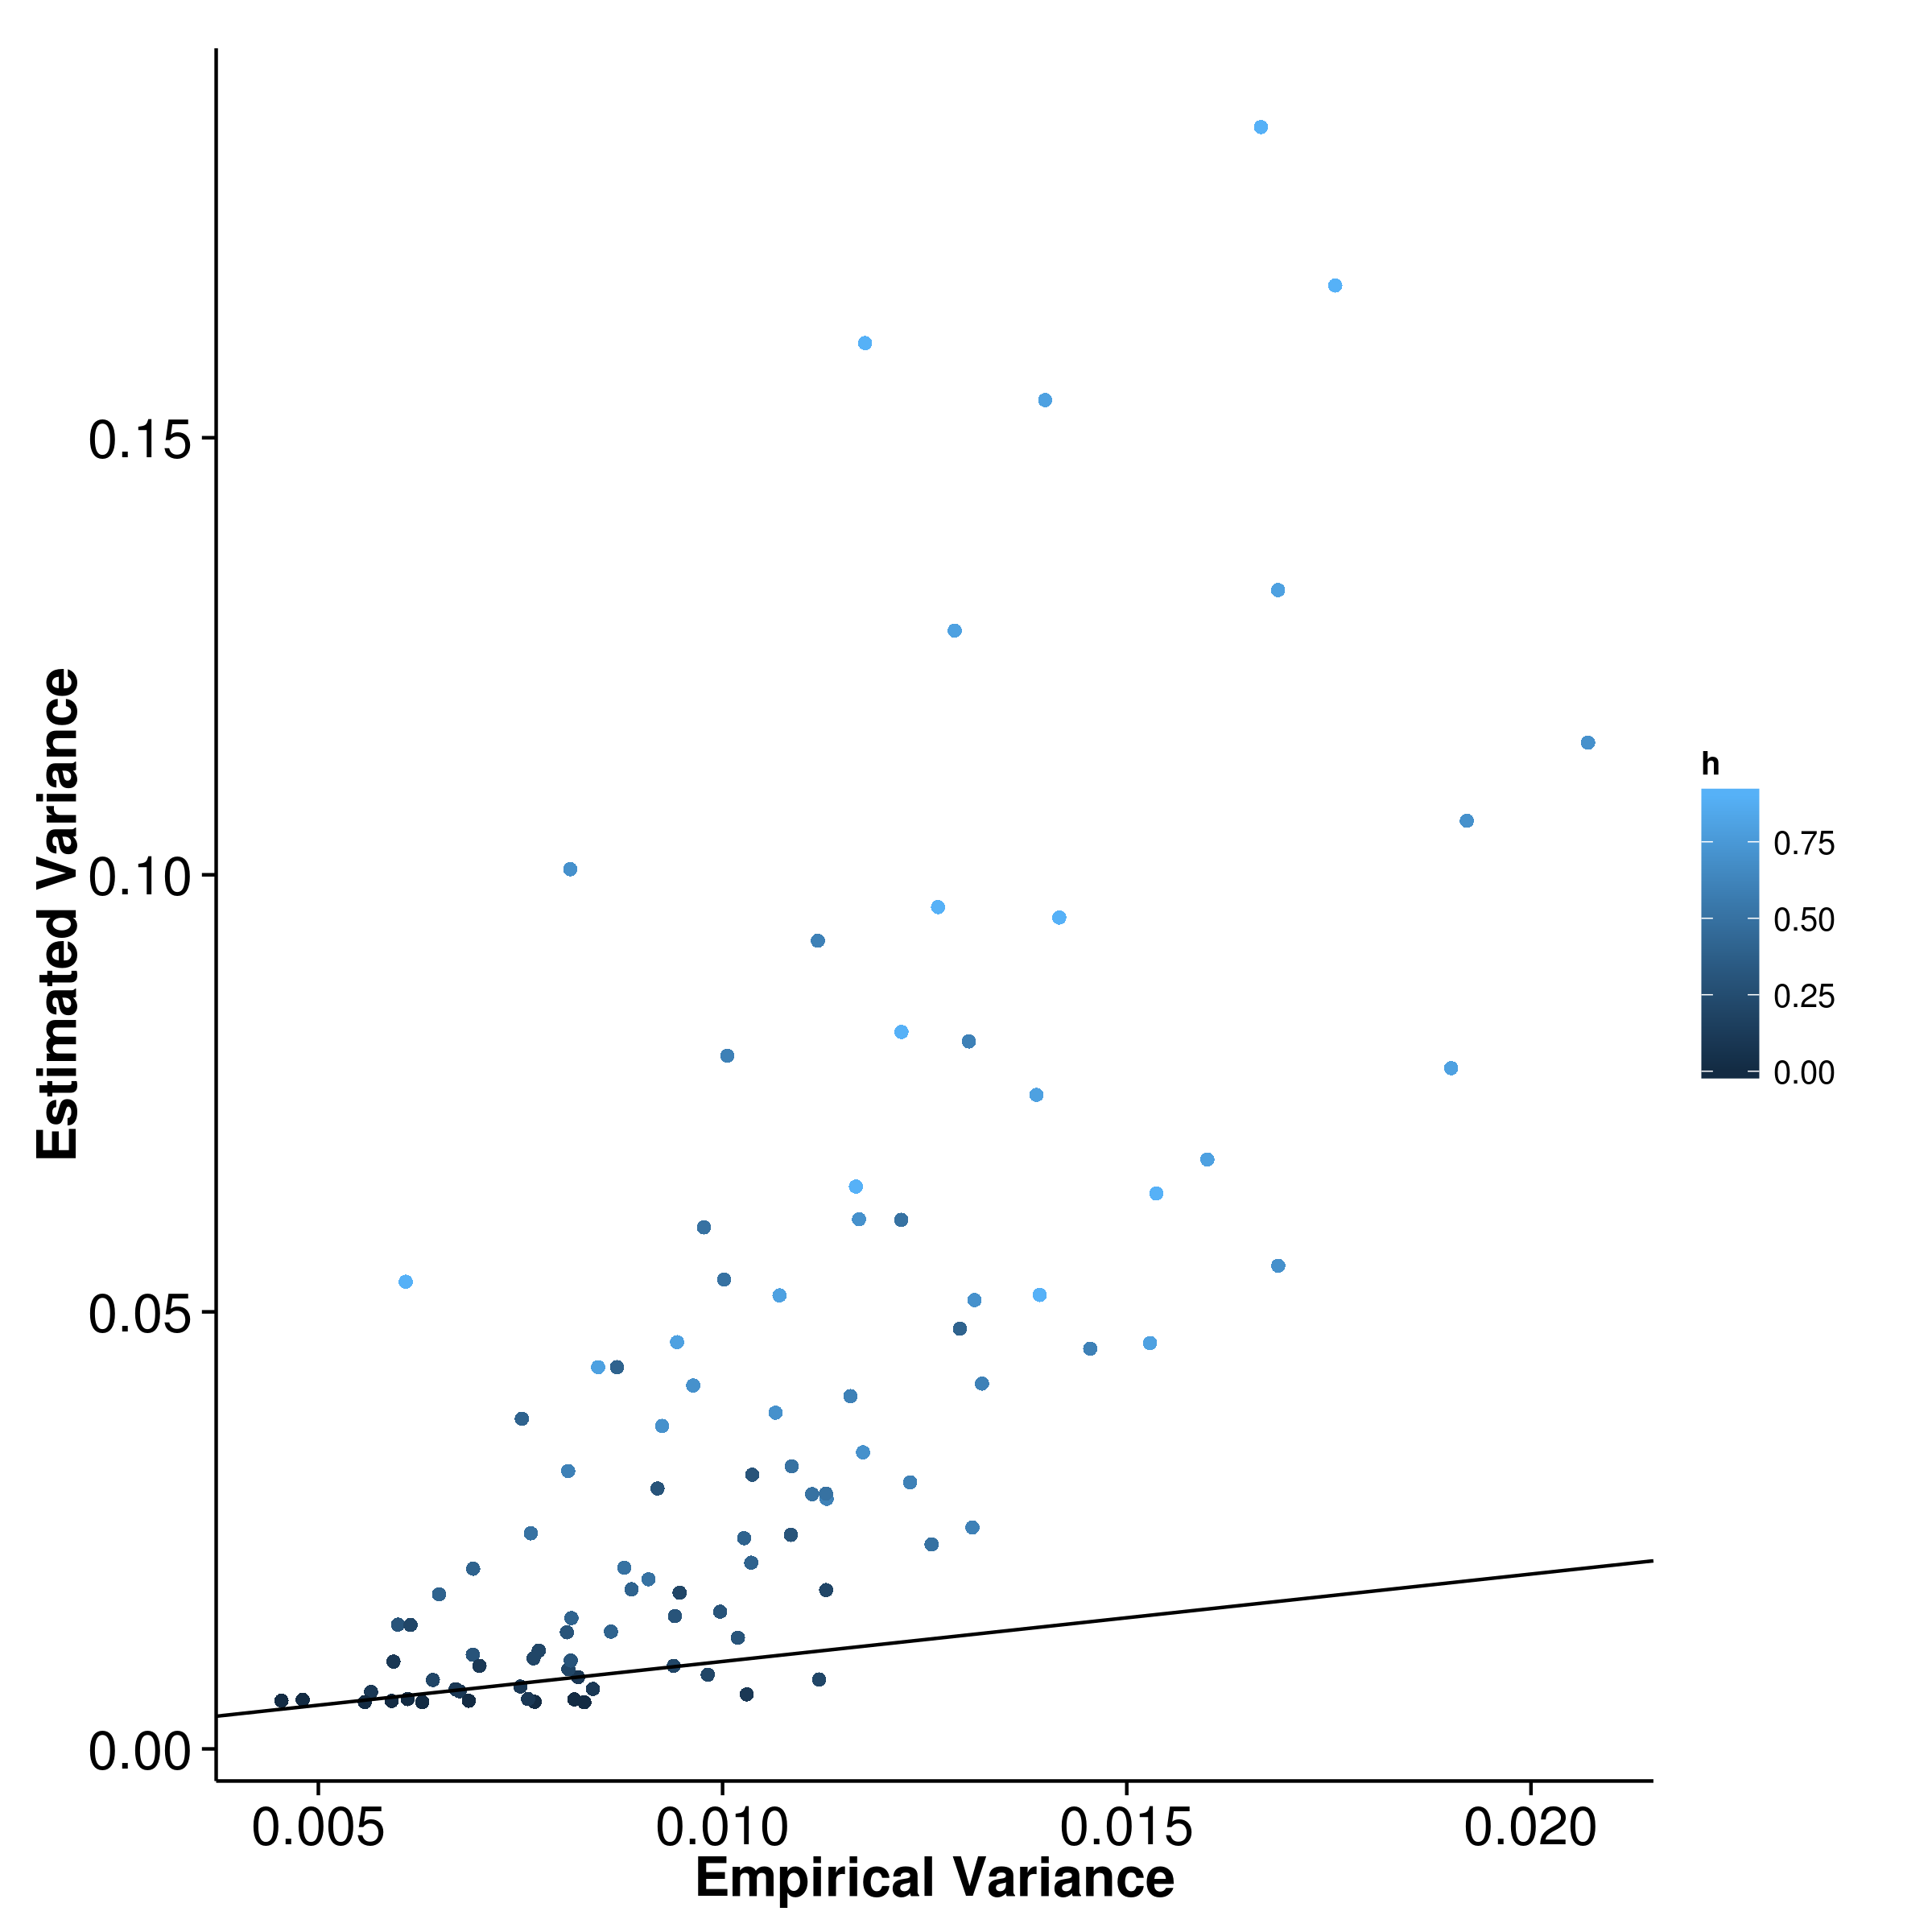
\includegraphics{figure/quantitative/same_effect/10c/ldsc_50k_10c_varH.png}}
			\label{fig:50k10cQtvarL}
		}
		\subfloat[LDSC with intercept estimation]{
			\scalebox{.4}{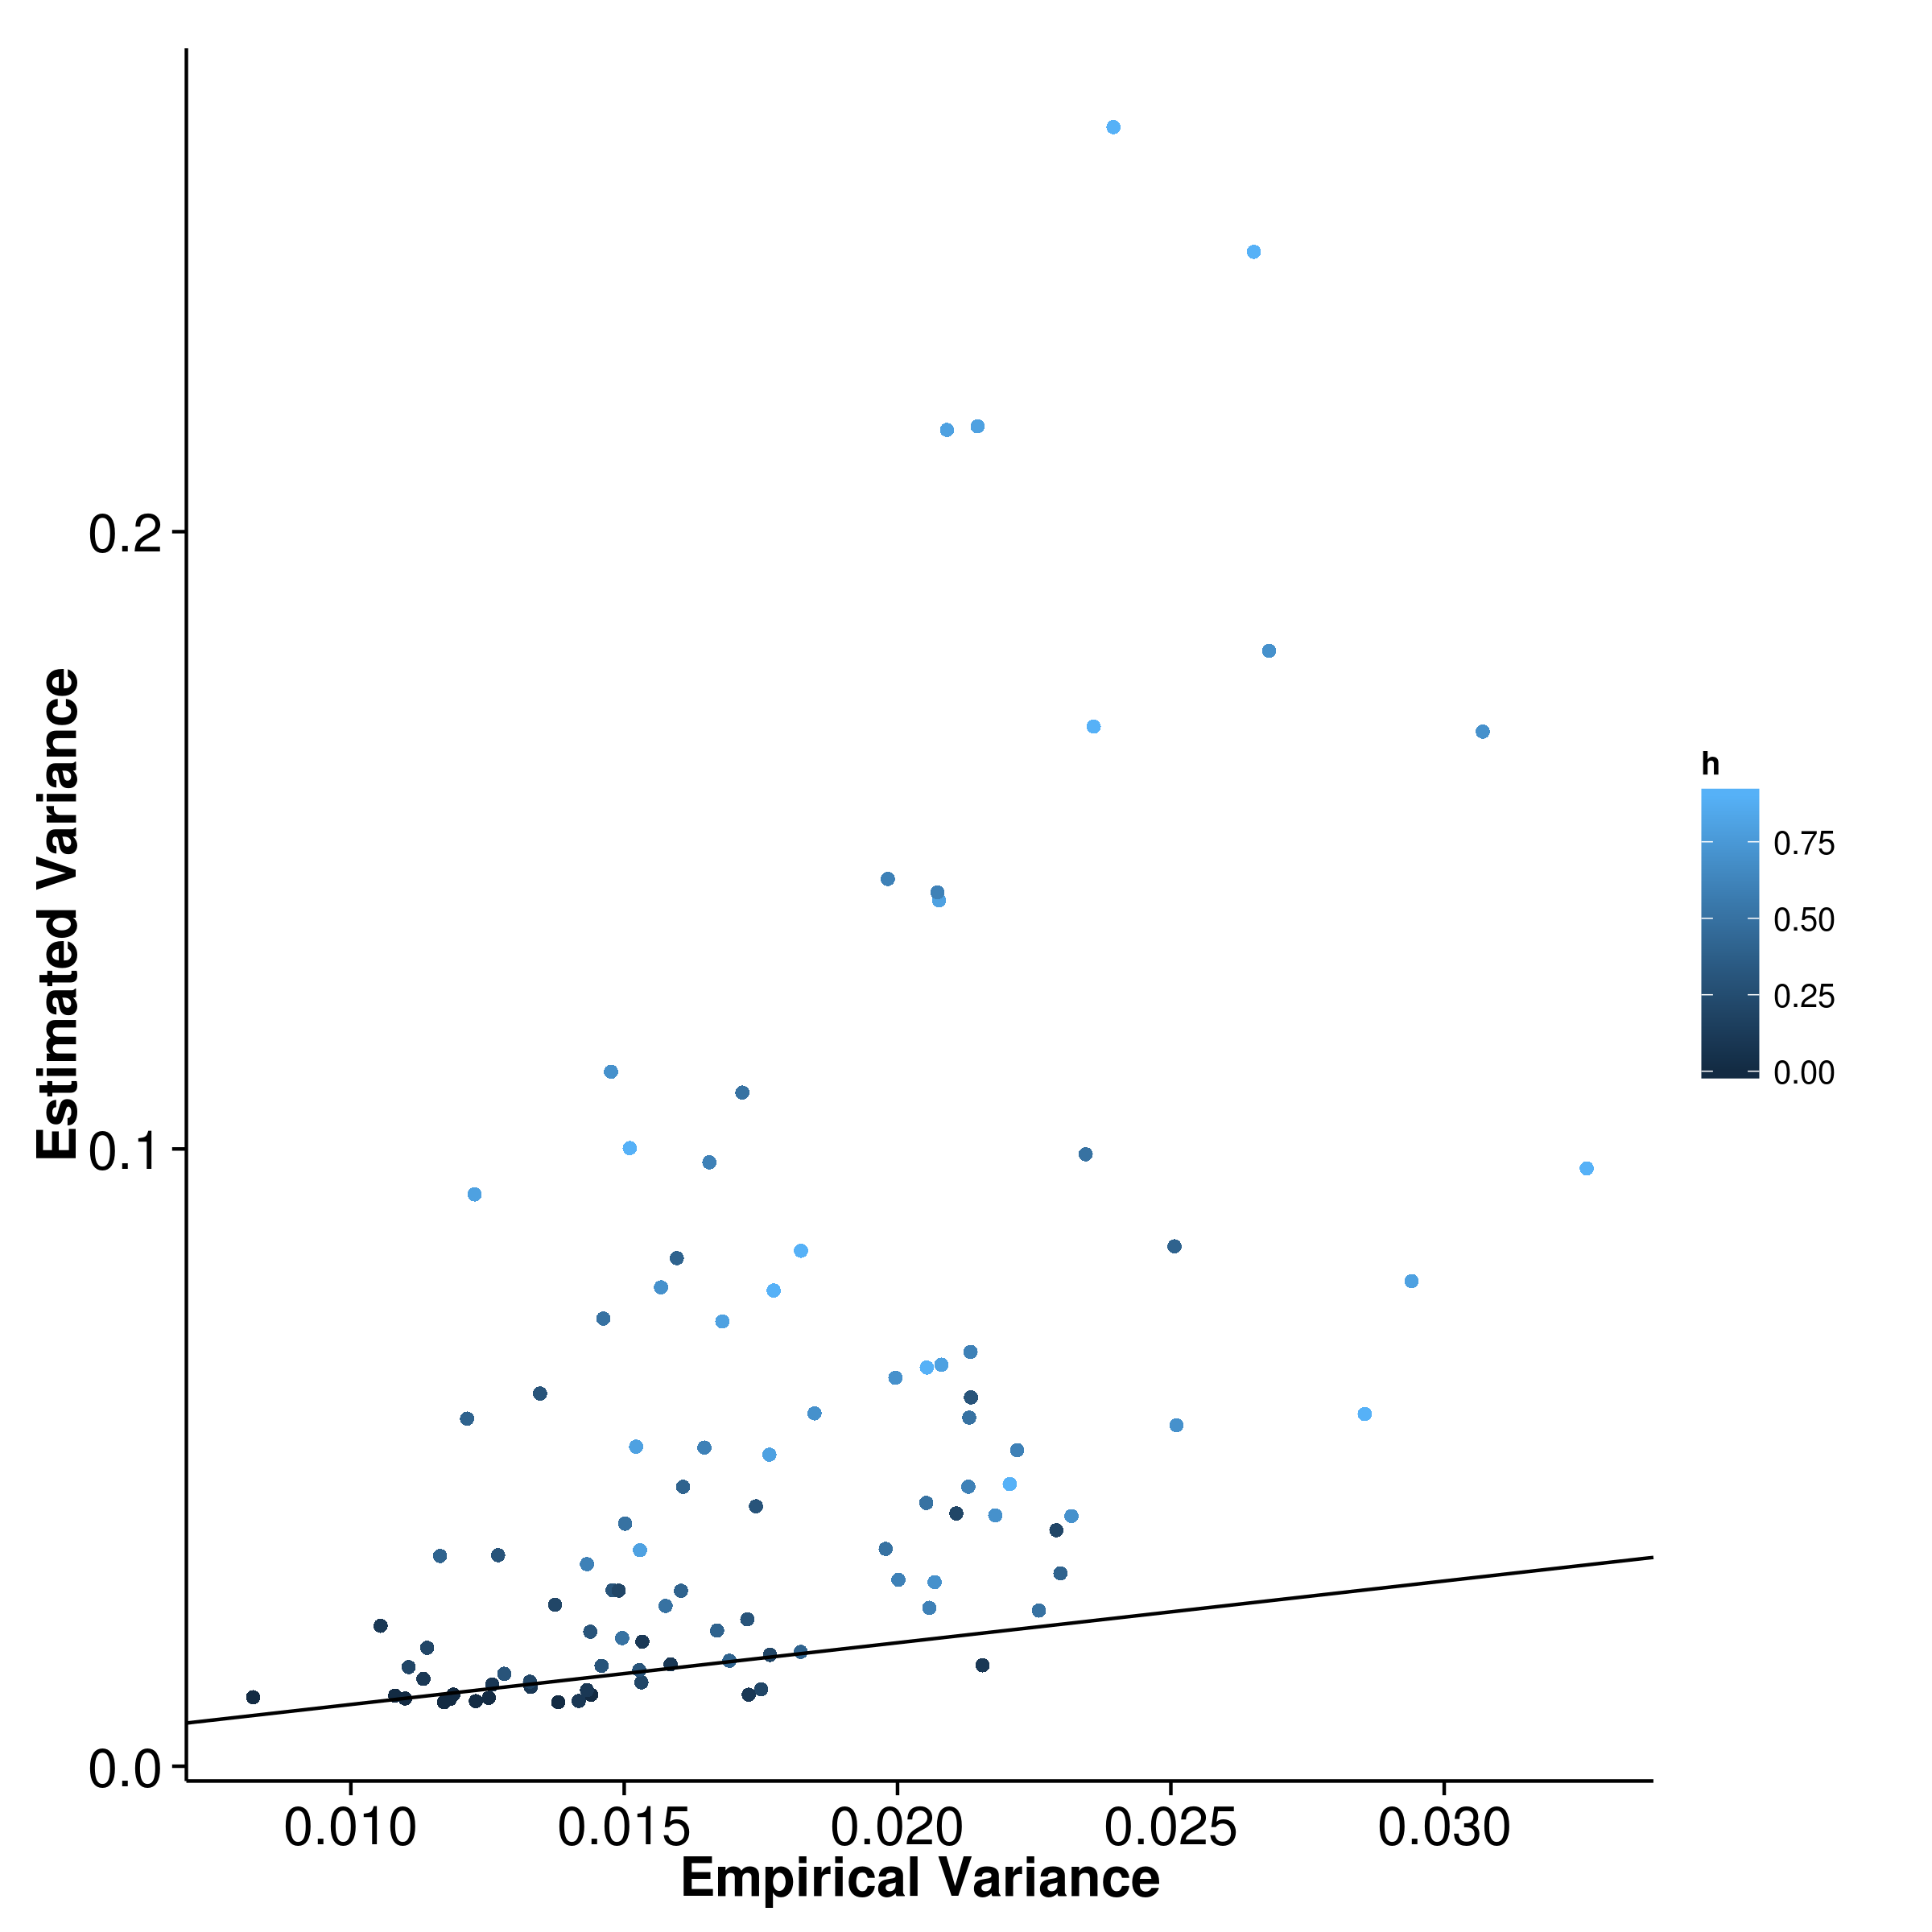
\includegraphics{figure/quantitative/same_effect/10c/ldscIn_50k_10c_varH.png}}
			\label{fig:50k10cQtvarI}
		}
		\label{fig:50k10cQtVar}
	\end{figure}
	
	
	\begin{figure}
		\centering
		\subfloat[SHREK]{
			\scalebox{.4}{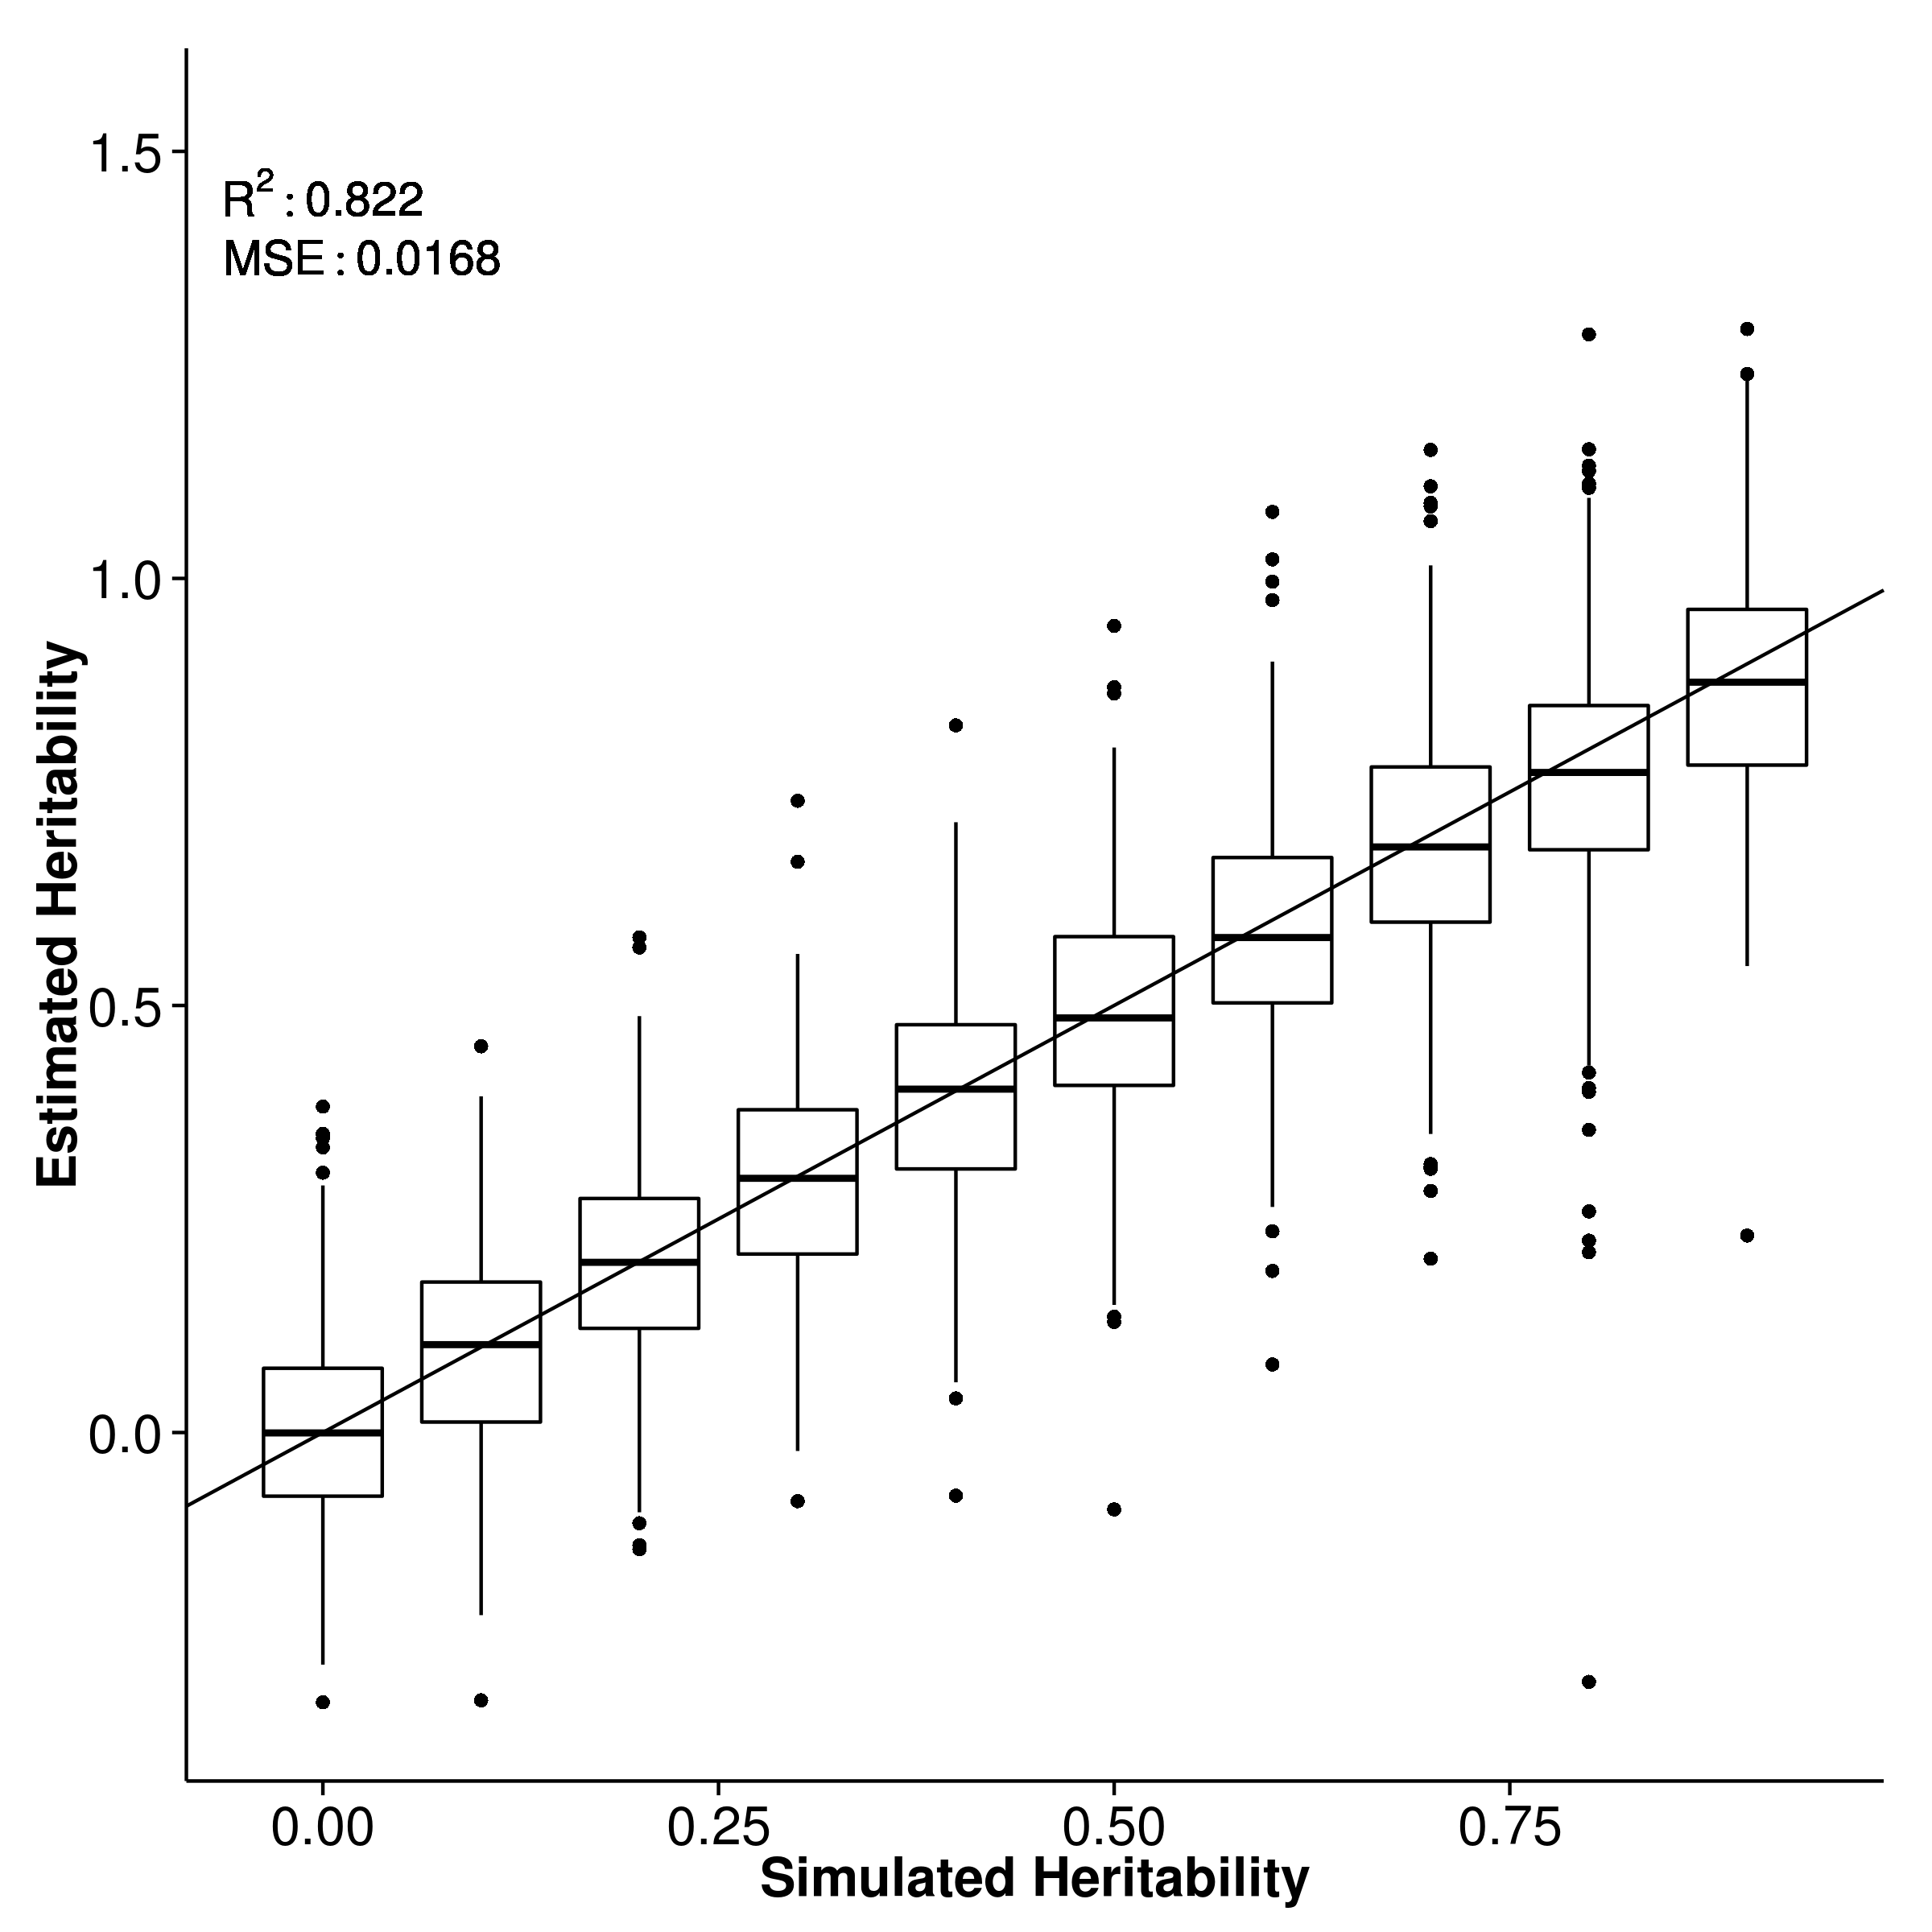
\includegraphics{figure/quantitative/same_effect/50c/shrek_50k_50c_meanH.png}}
			\label{fig:50k50cQtmeanS}
		}
		\subfloat[GCTA]{
			\scalebox{.4}{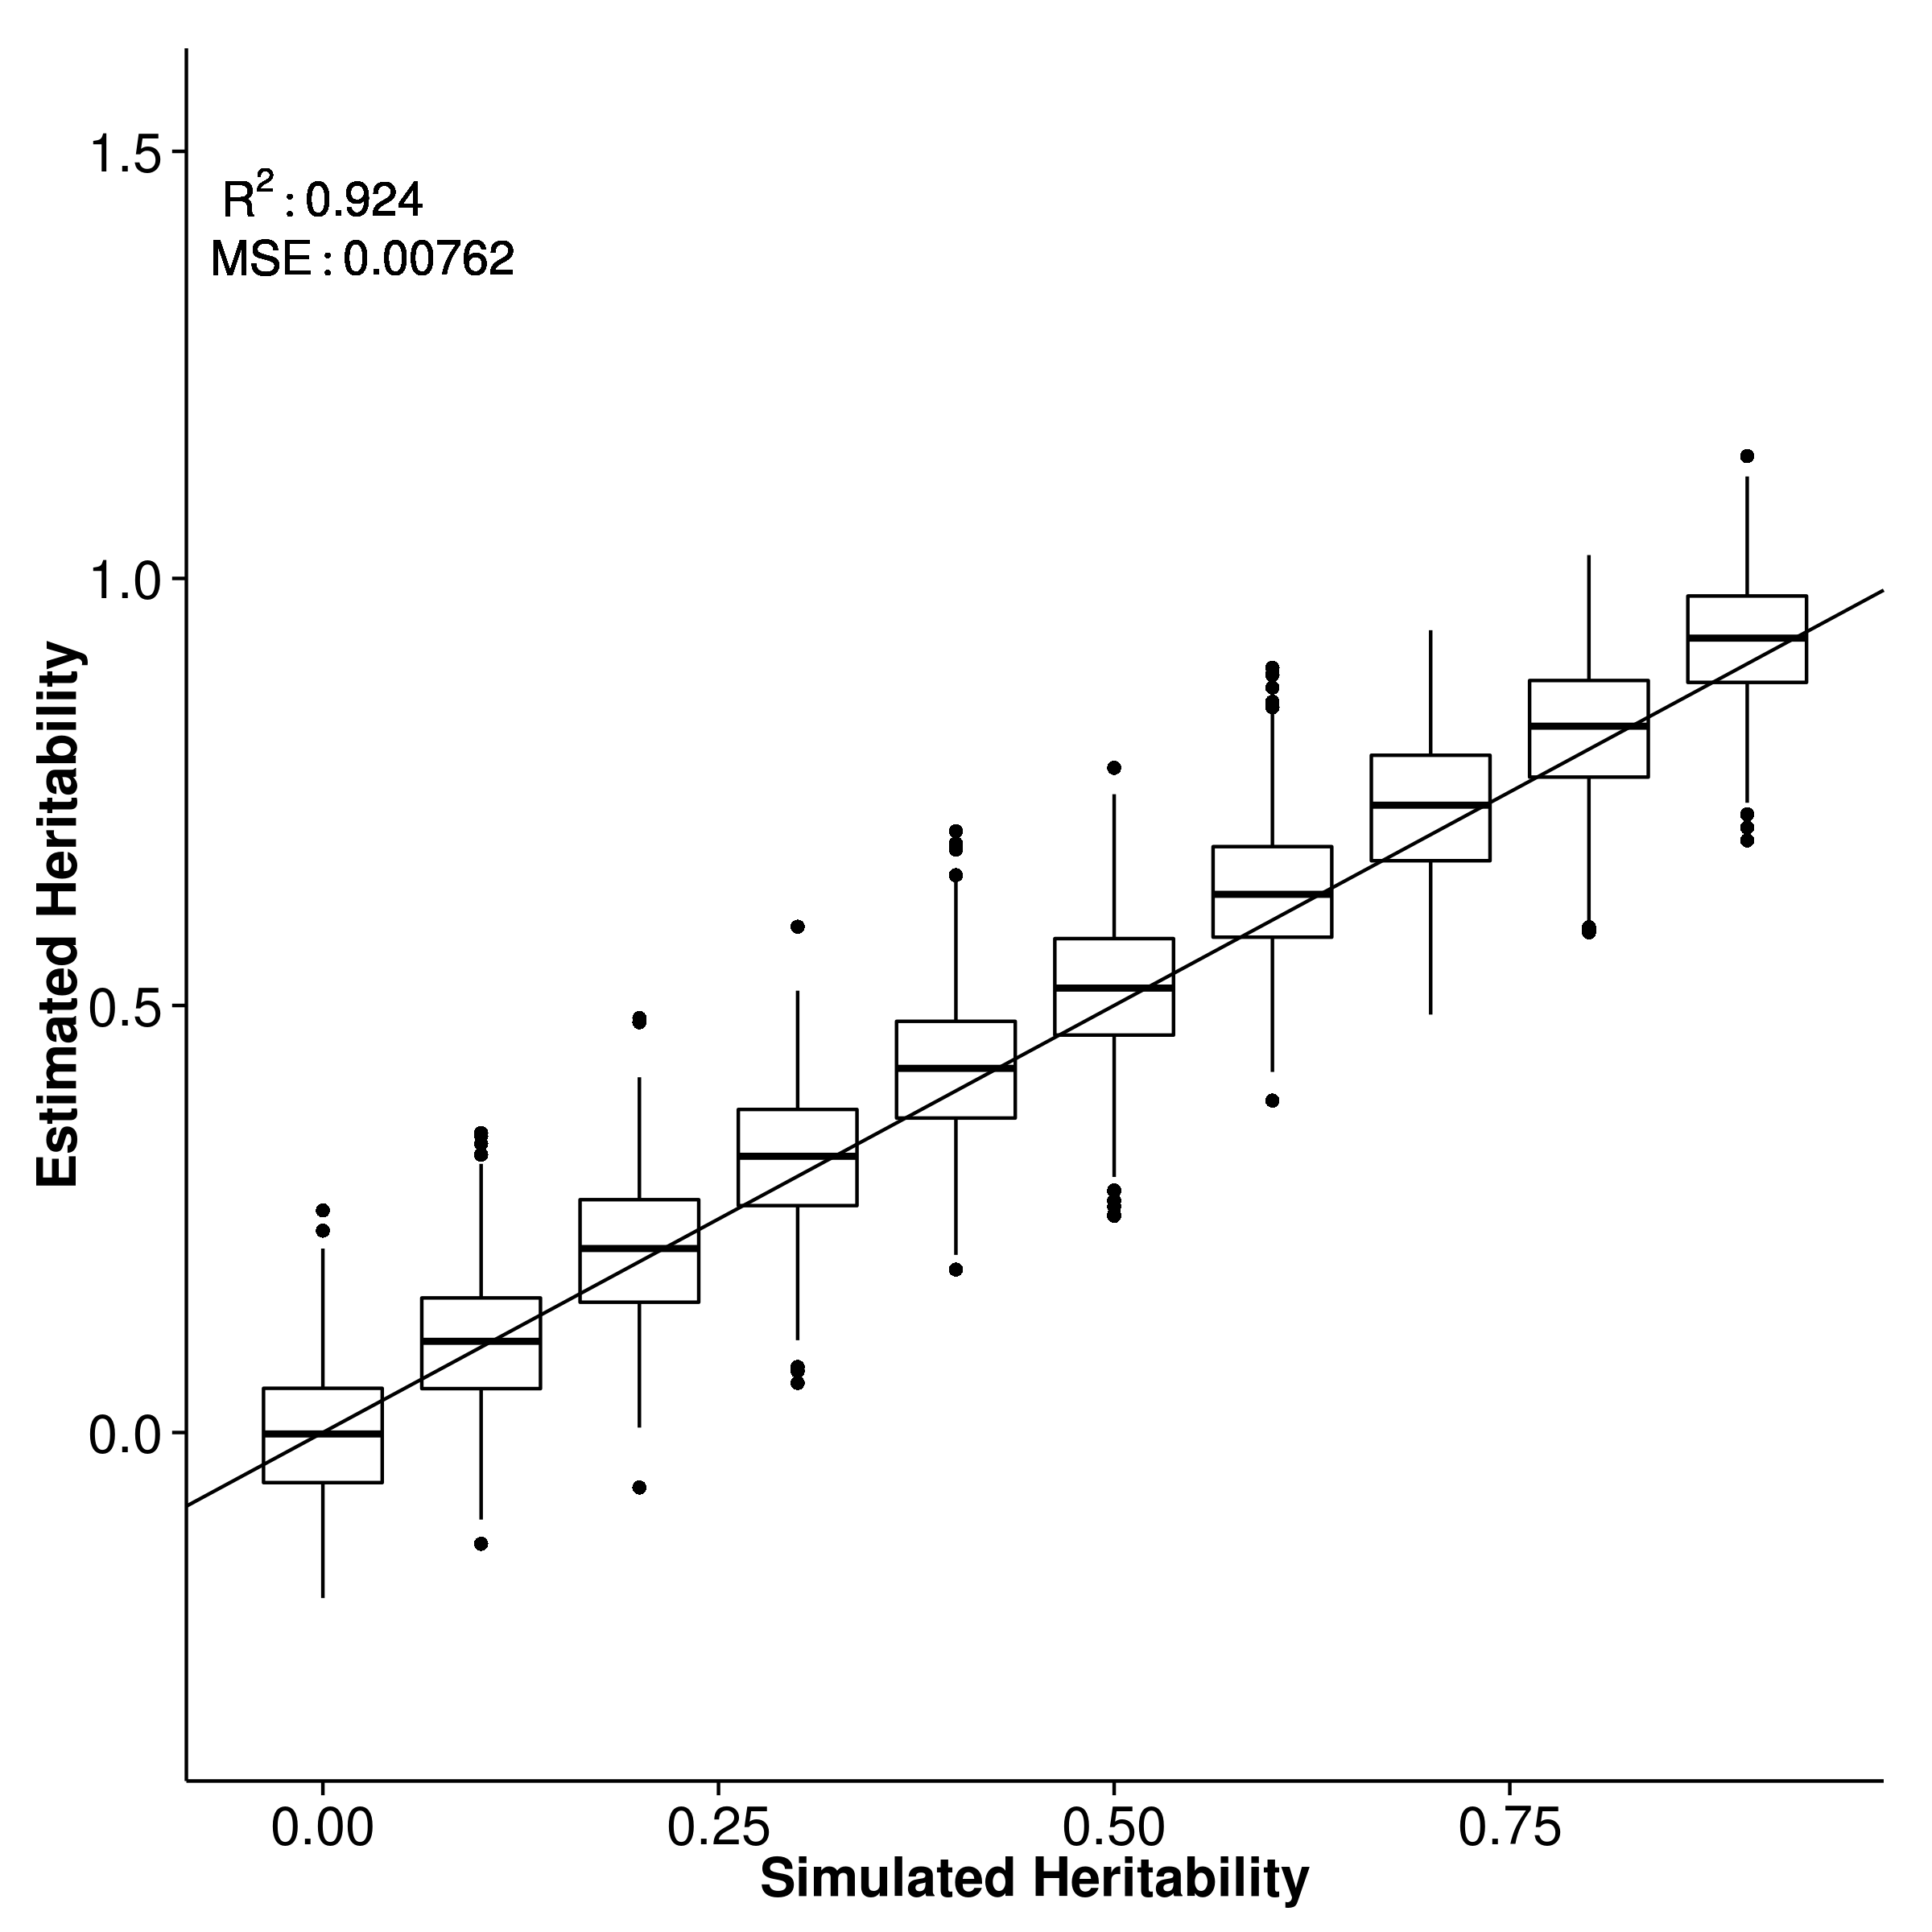
\includegraphics{figure/quantitative/same_effect/50c/gcta_50k_50c_meanH.png}}
			\label{fig:50k50cQtmeanG}
		}\\
		\subfloat[LDSC with fix intercept]{
			\scalebox{.4}{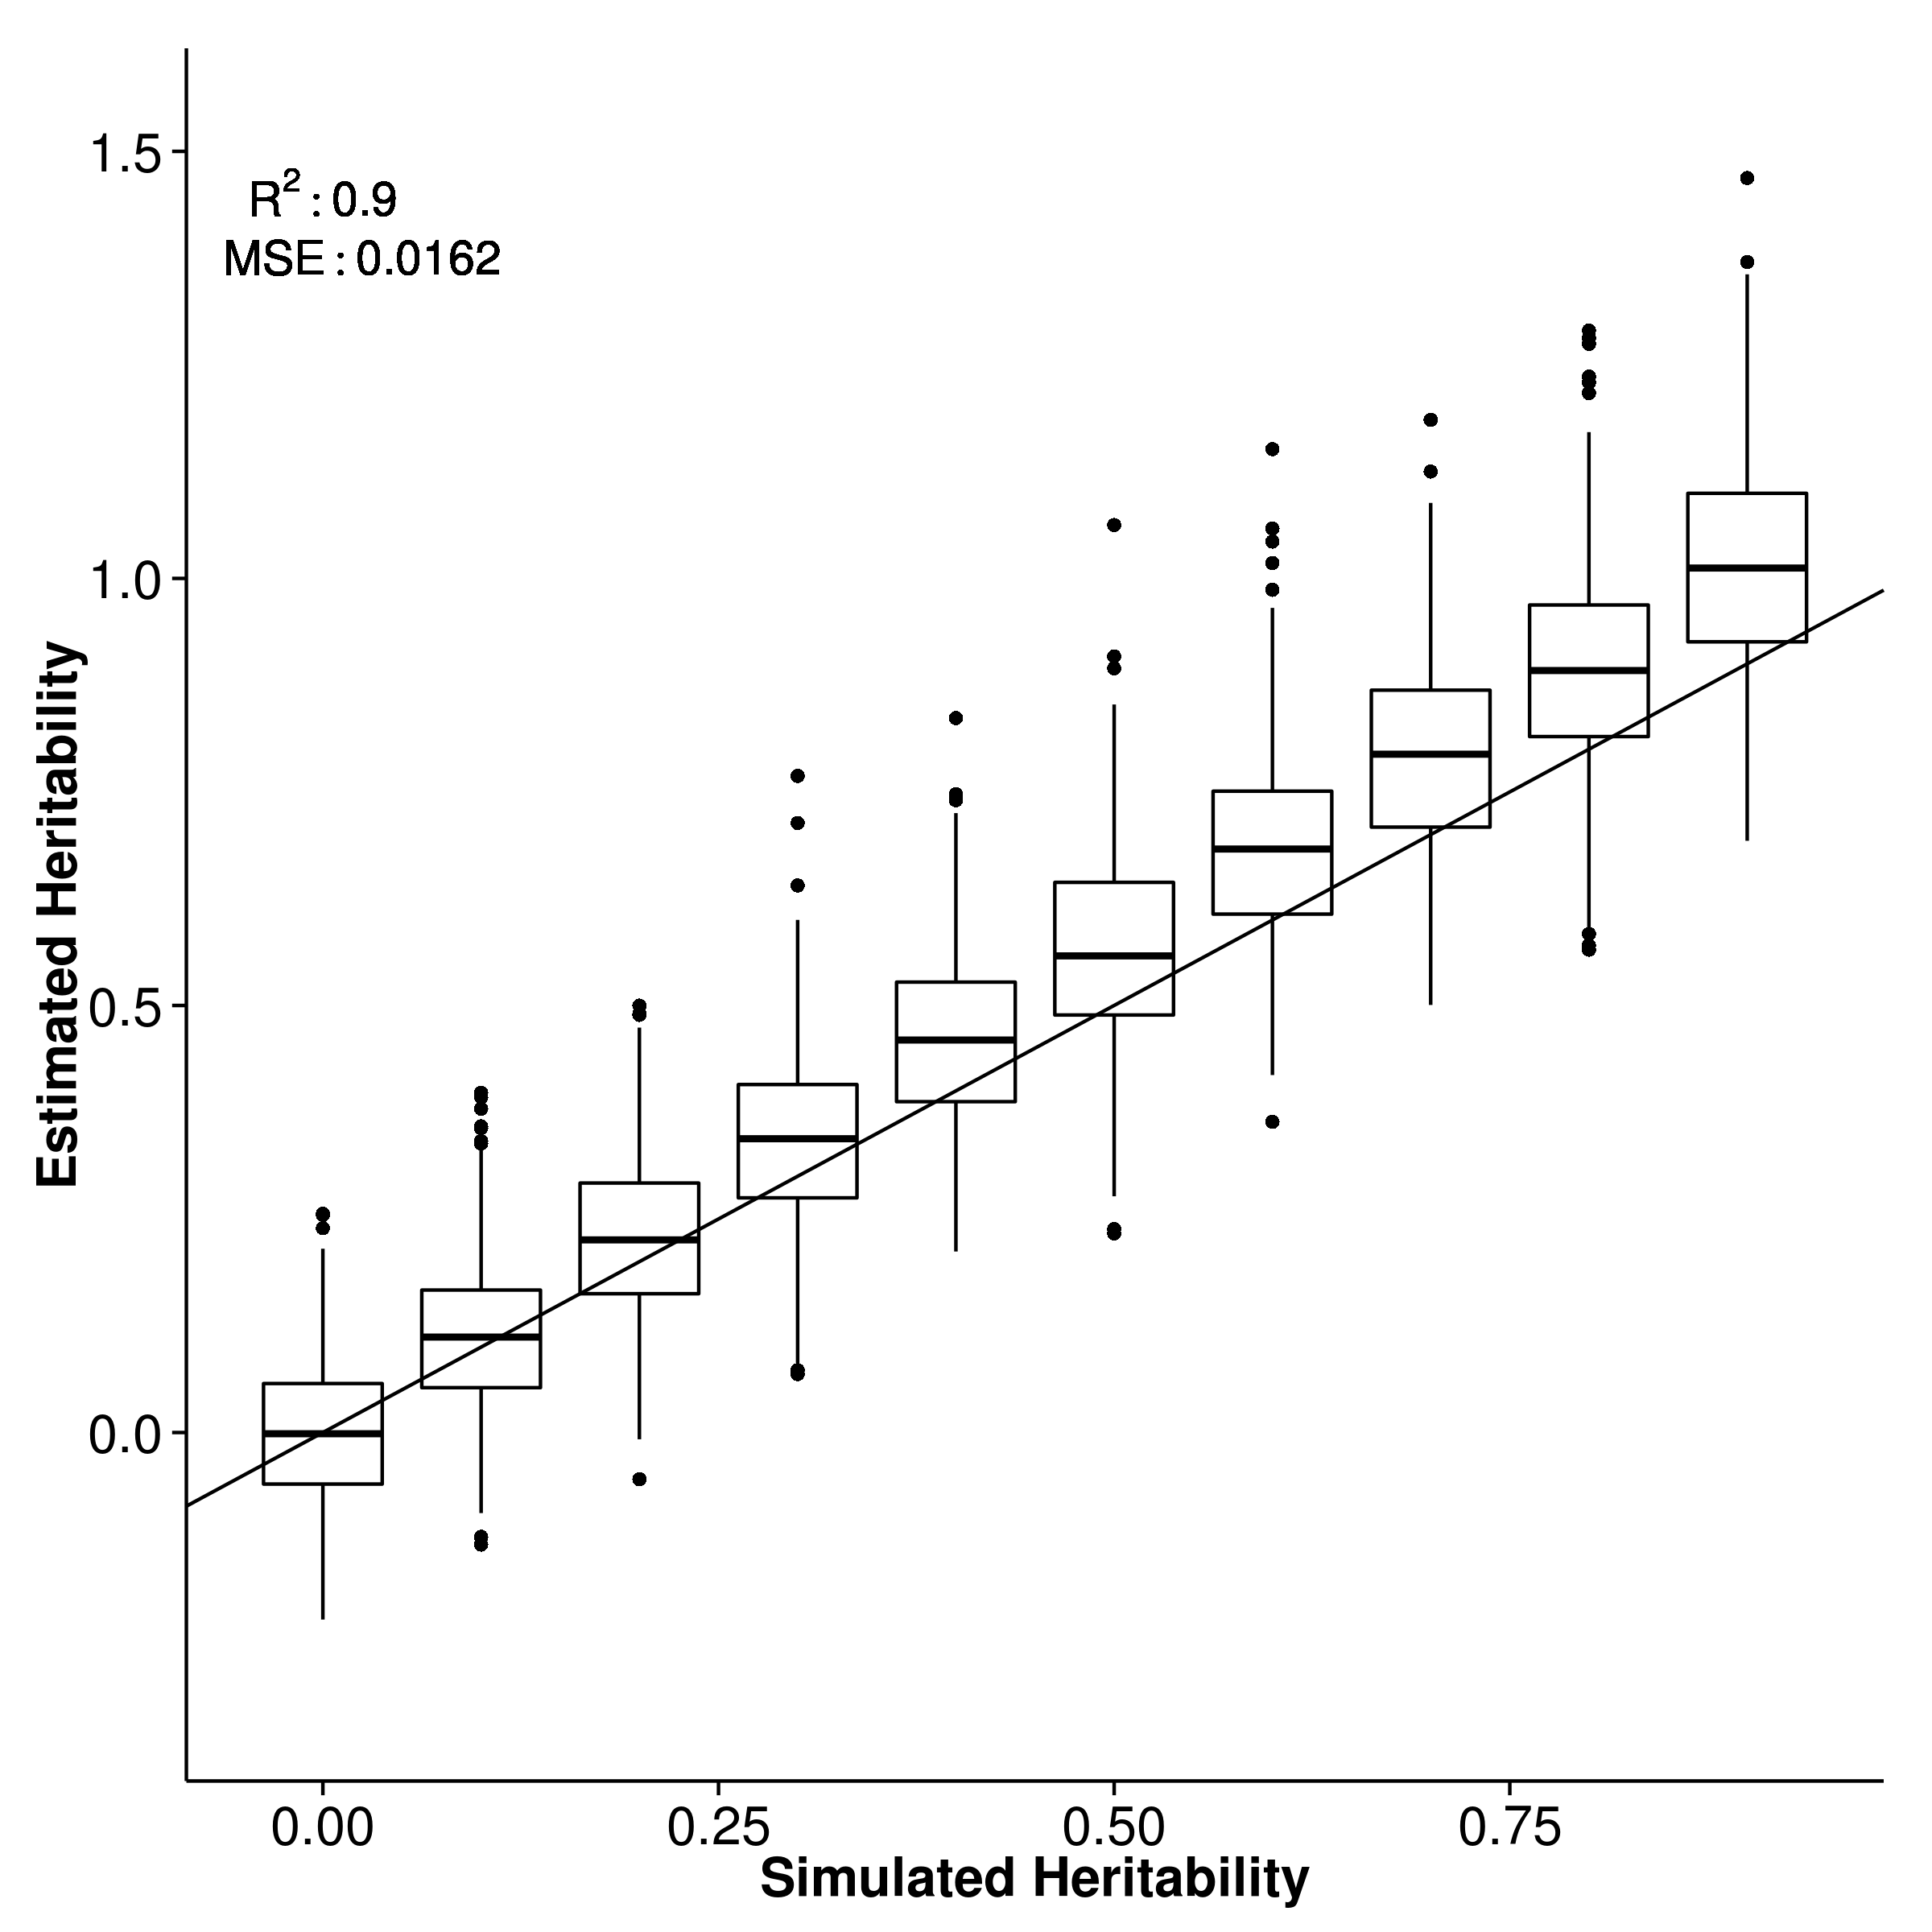
\includegraphics{figure/quantitative/same_effect/50c/ldsc_50k_50c_meanH.png}}
			\label{fig:50k50cQtmeanL}
		}
		\subfloat[LDSC with intercept estimation]{
			\scalebox{.4}{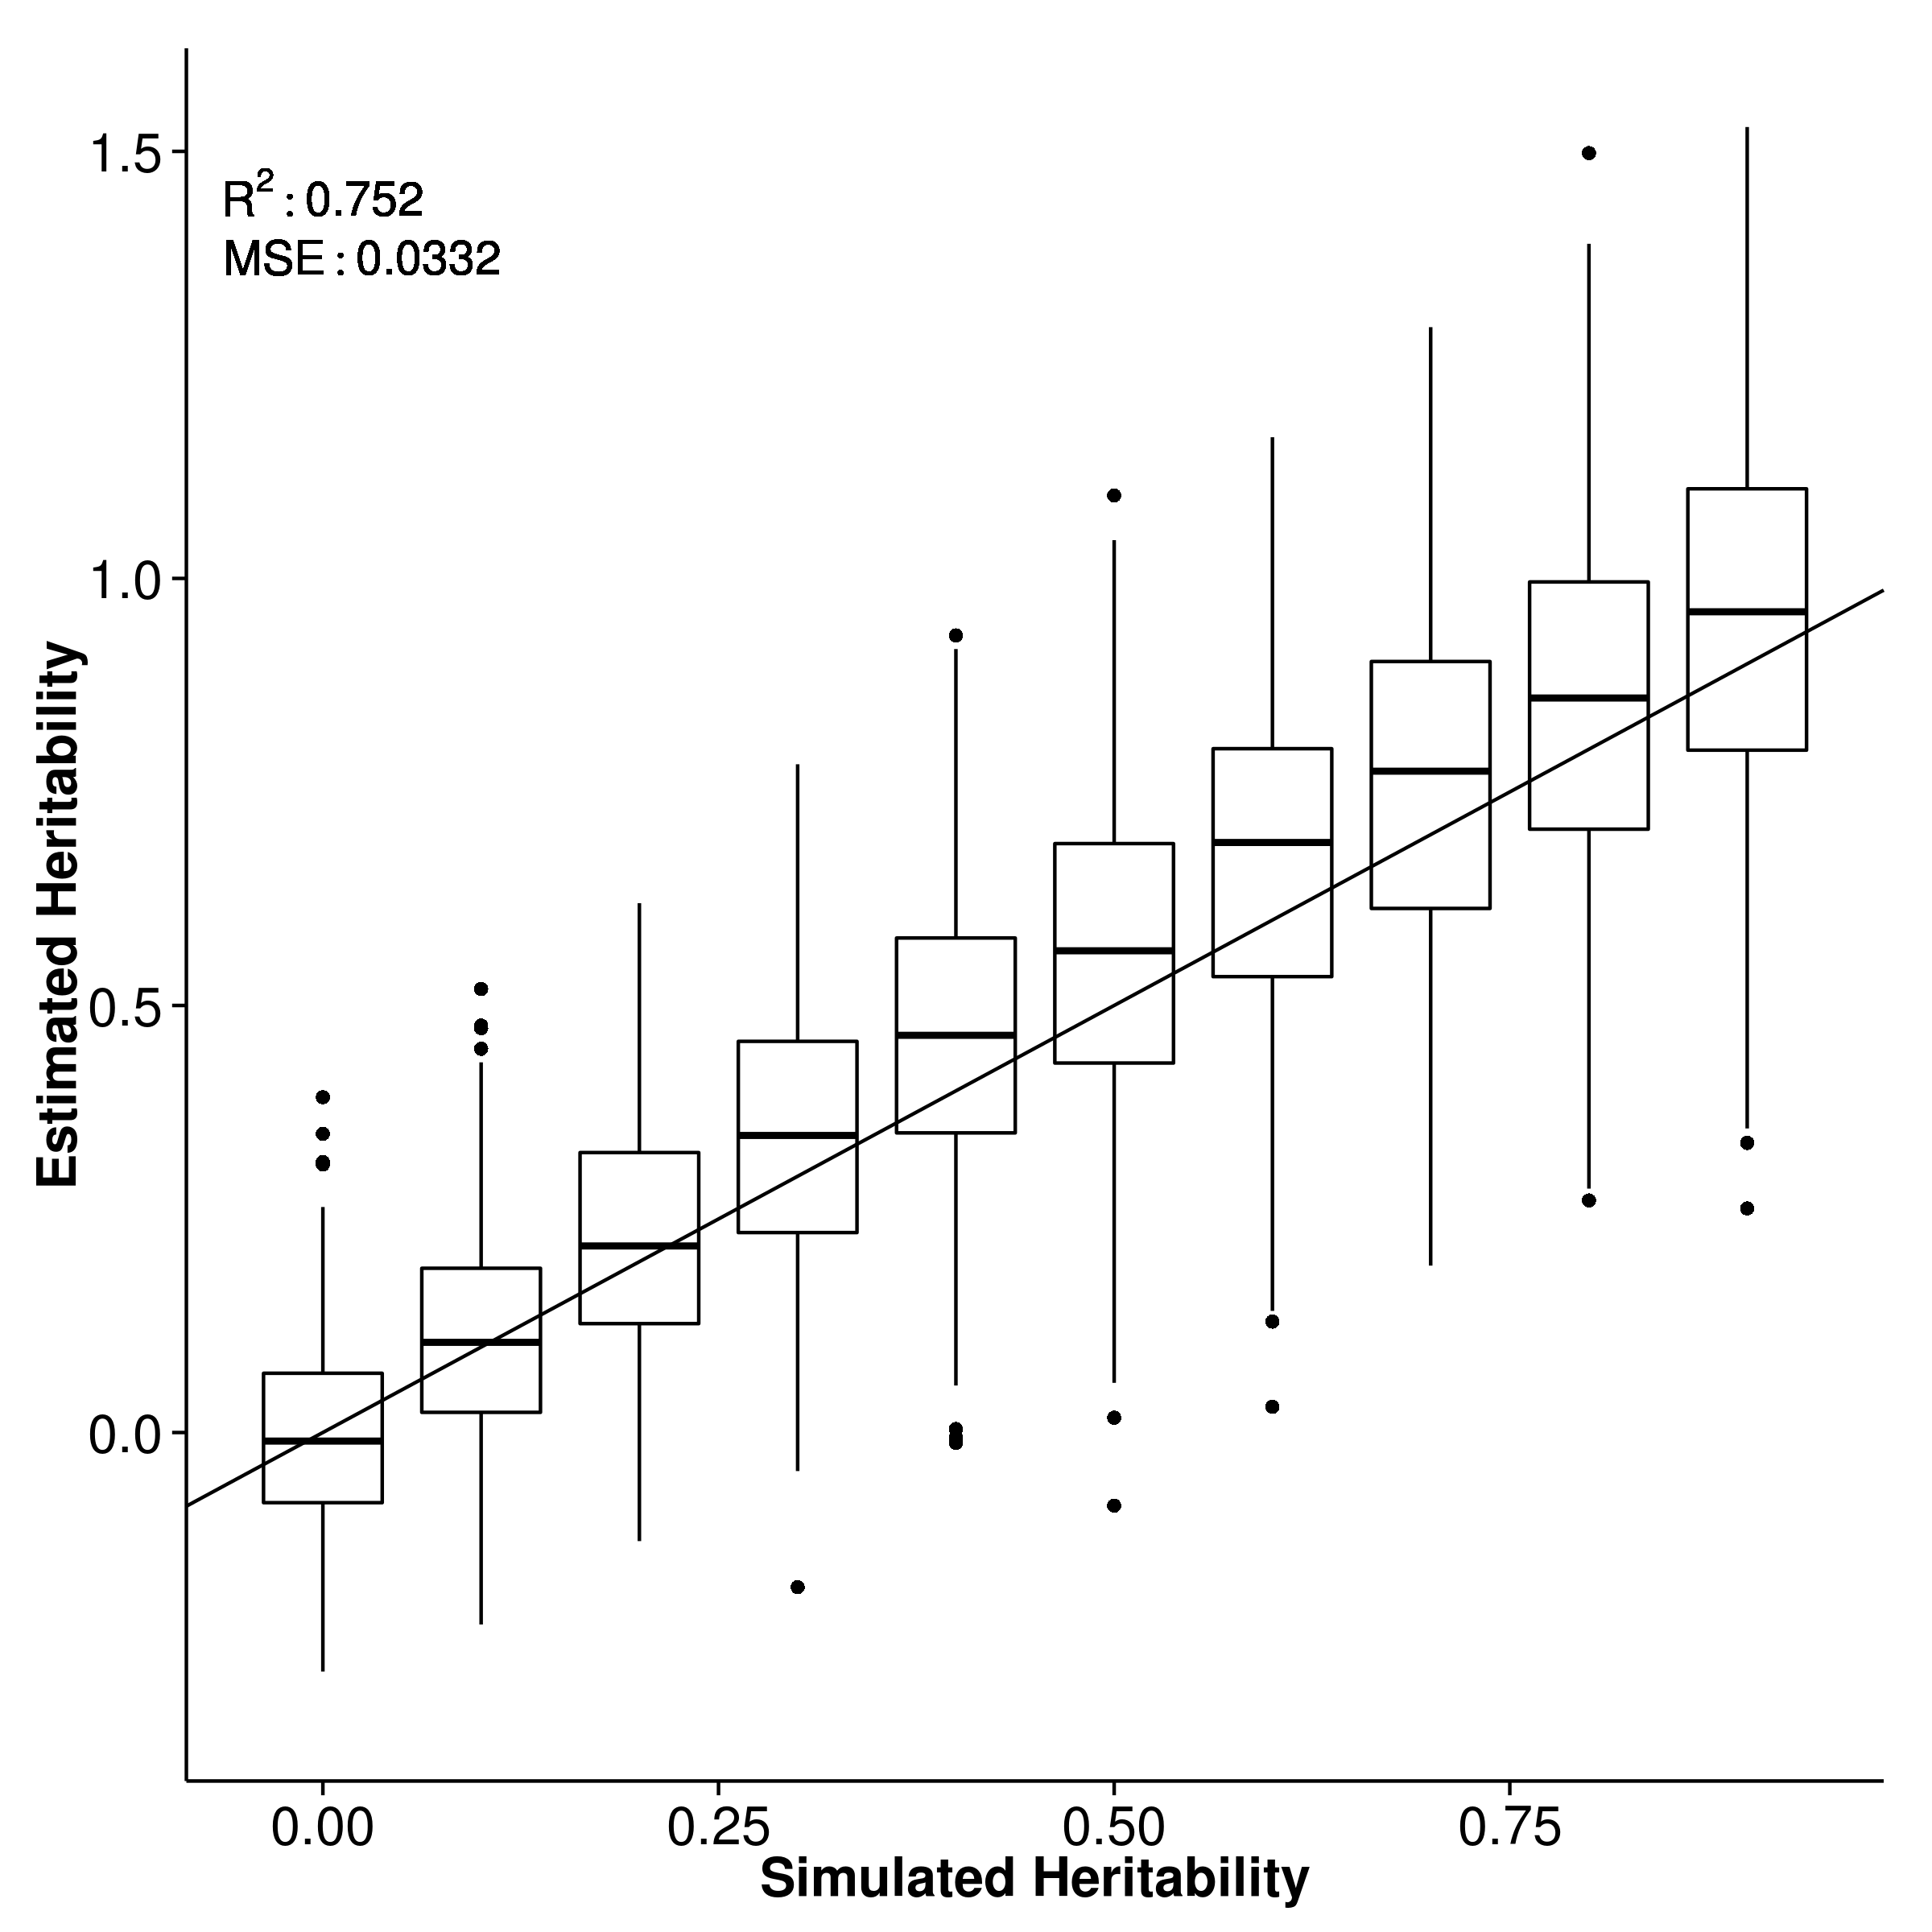
\includegraphics{figure/quantitative/same_effect/50c/ldscIn_50k_50c_meanH.png}}
			\label{fig:50k50cQtmeanI}
		}
		\caption[Simulation of Quantitative Traits with 50k \glsentryshortpl{SNP} and 50 causal variants of same effect size]
		{Simulation of Quantitative Traits with 50k \glsentryshortpl{SNP} and 50 causal variants with same effect size.} 
		\label{fig:50k50cQtMean}
	\end{figure}
	\begin{figure}
		\centering
		\subfloat[SHREK]{
			\scalebox{.4}{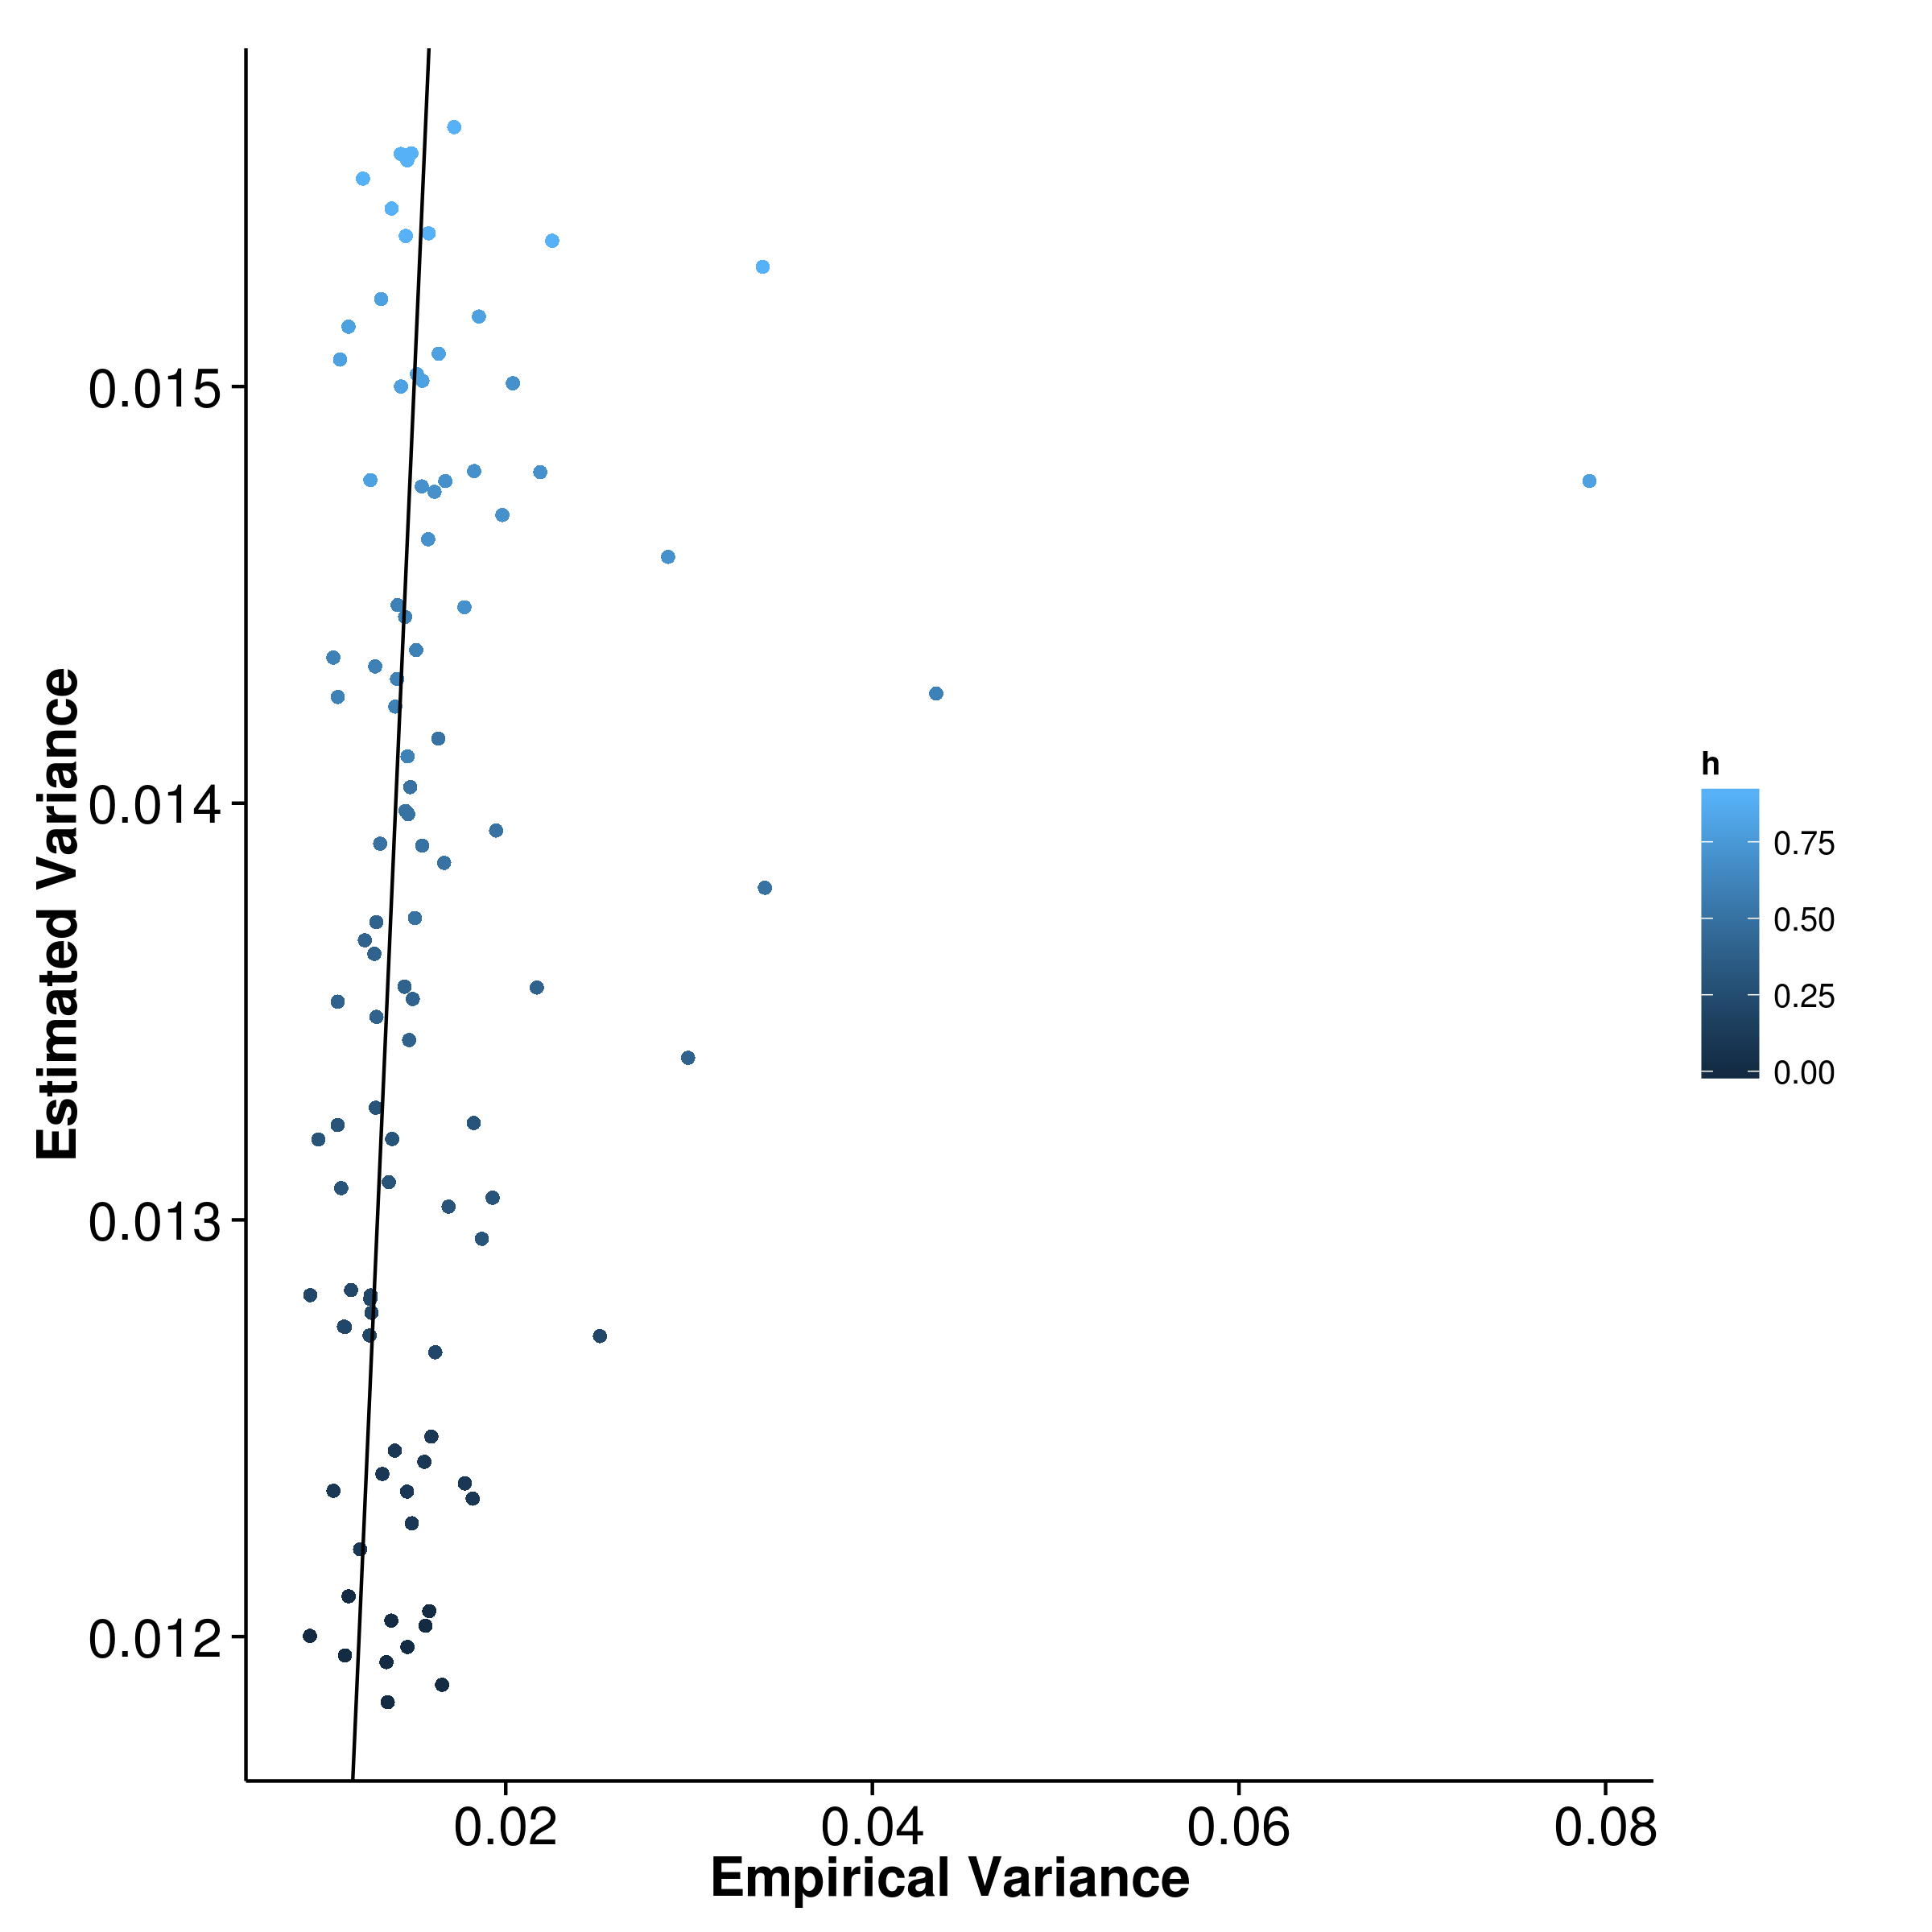
\includegraphics{figure/quantitative/same_effect/50c/shrek_50k_50c_varH.png}}
			\label{fig:50k50cQtvarS}
		}
		\subfloat[GCTA]{
			\scalebox{.4}{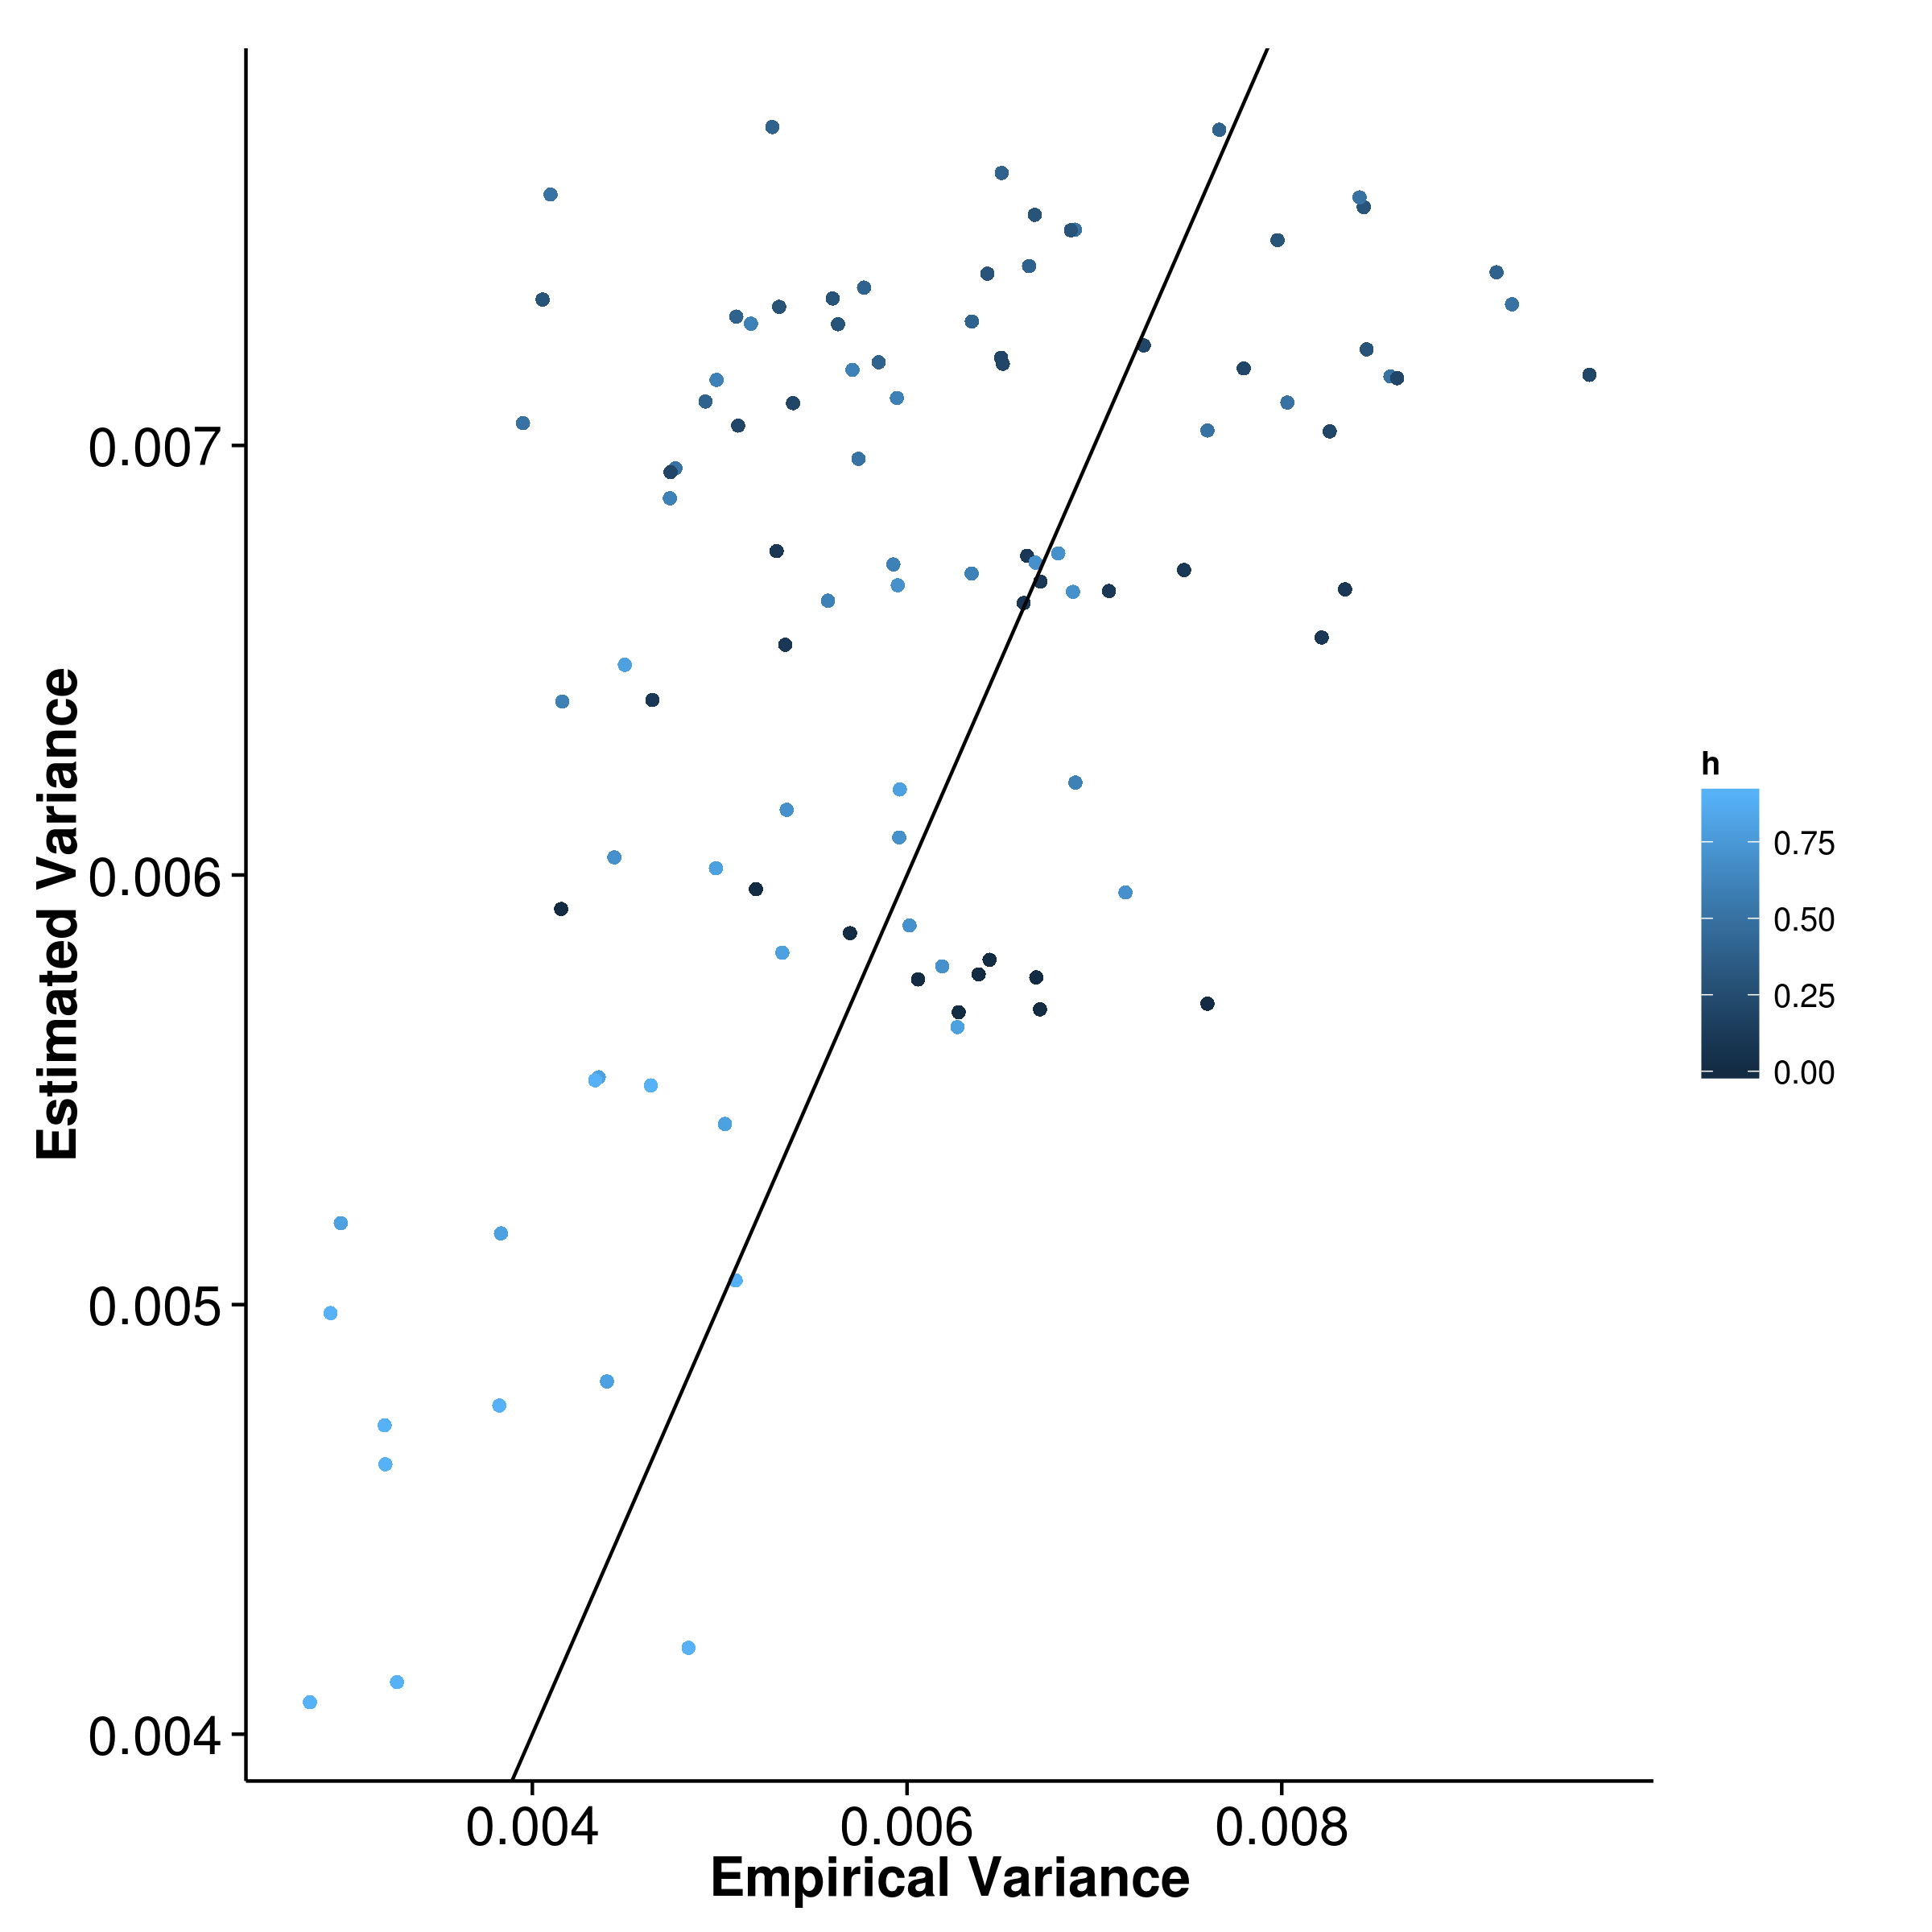
\includegraphics{figure/quantitative/same_effect/50c/gcta_50k_50c_varH.png}}
			\label{fig:50k50cQtvarG}
		}\\
		\subfloat[LDSC with fix intercept]{
			\scalebox{.4}{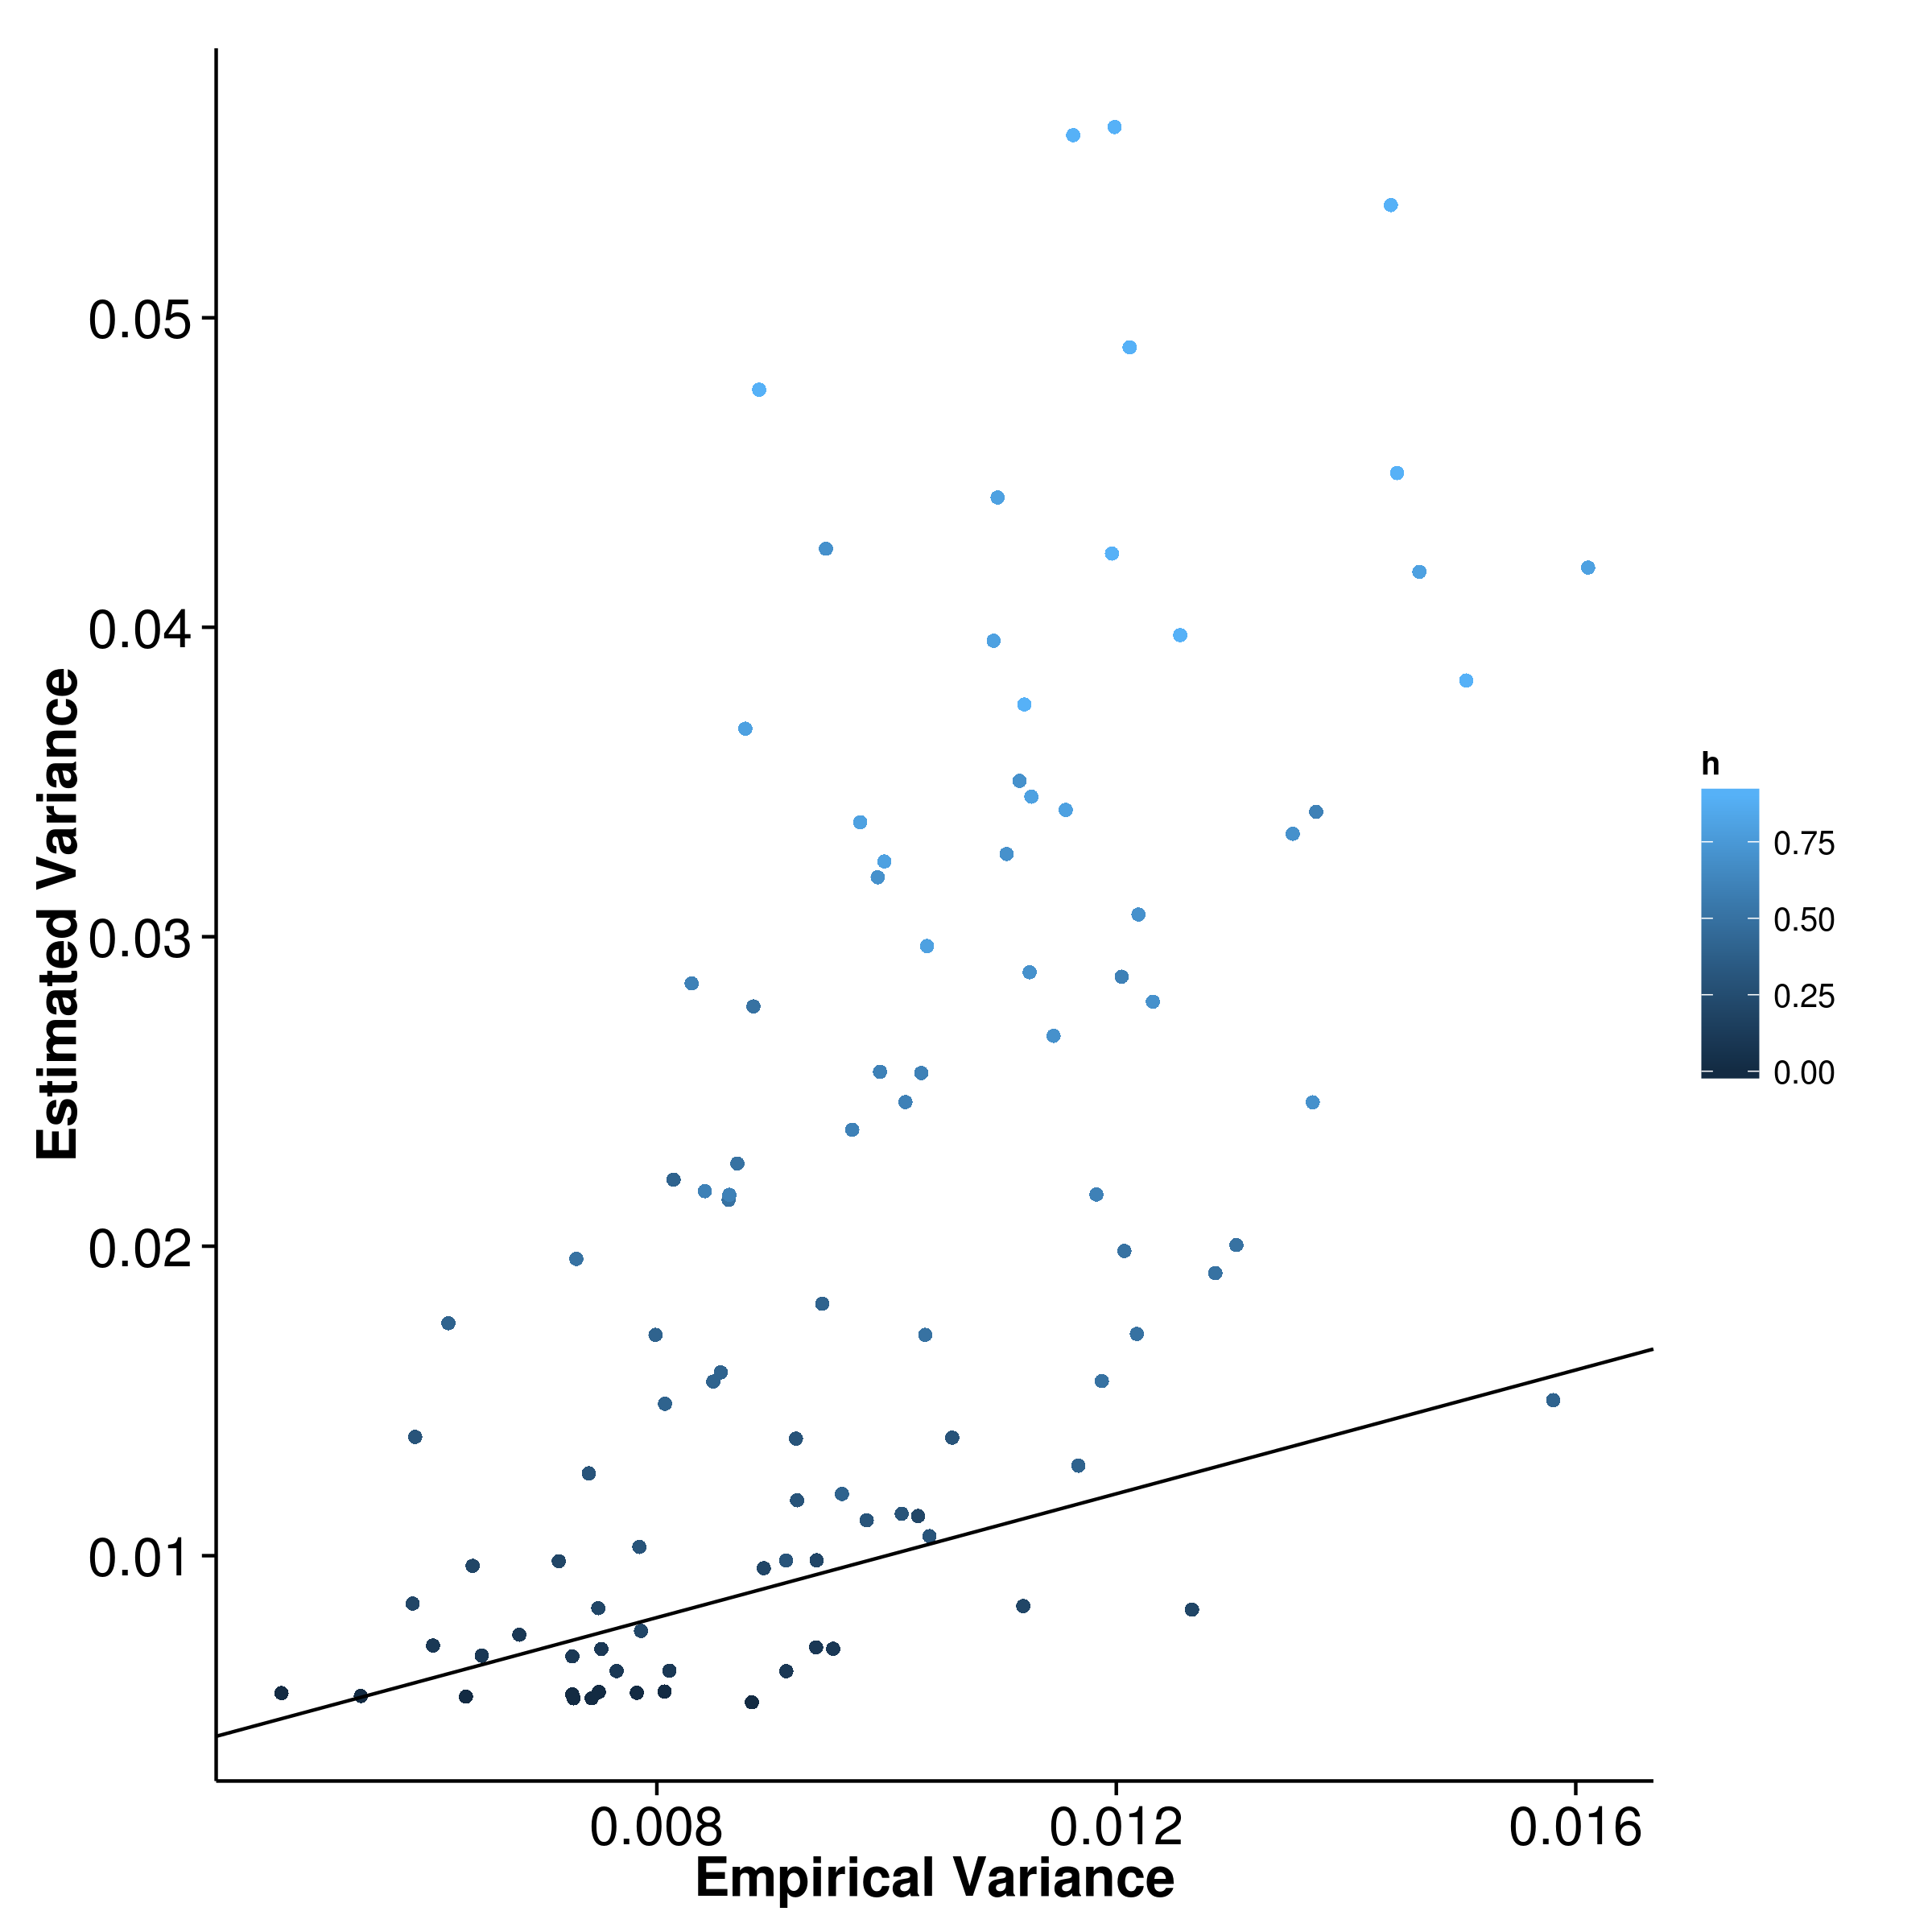
\includegraphics{figure/quantitative/same_effect/50c/ldsc_50k_50c_varH.png}}
			\label{fig:50k50cQtvarL}
		}
		\subfloat[LDSC with intercept estimation]{
			\scalebox{.4}{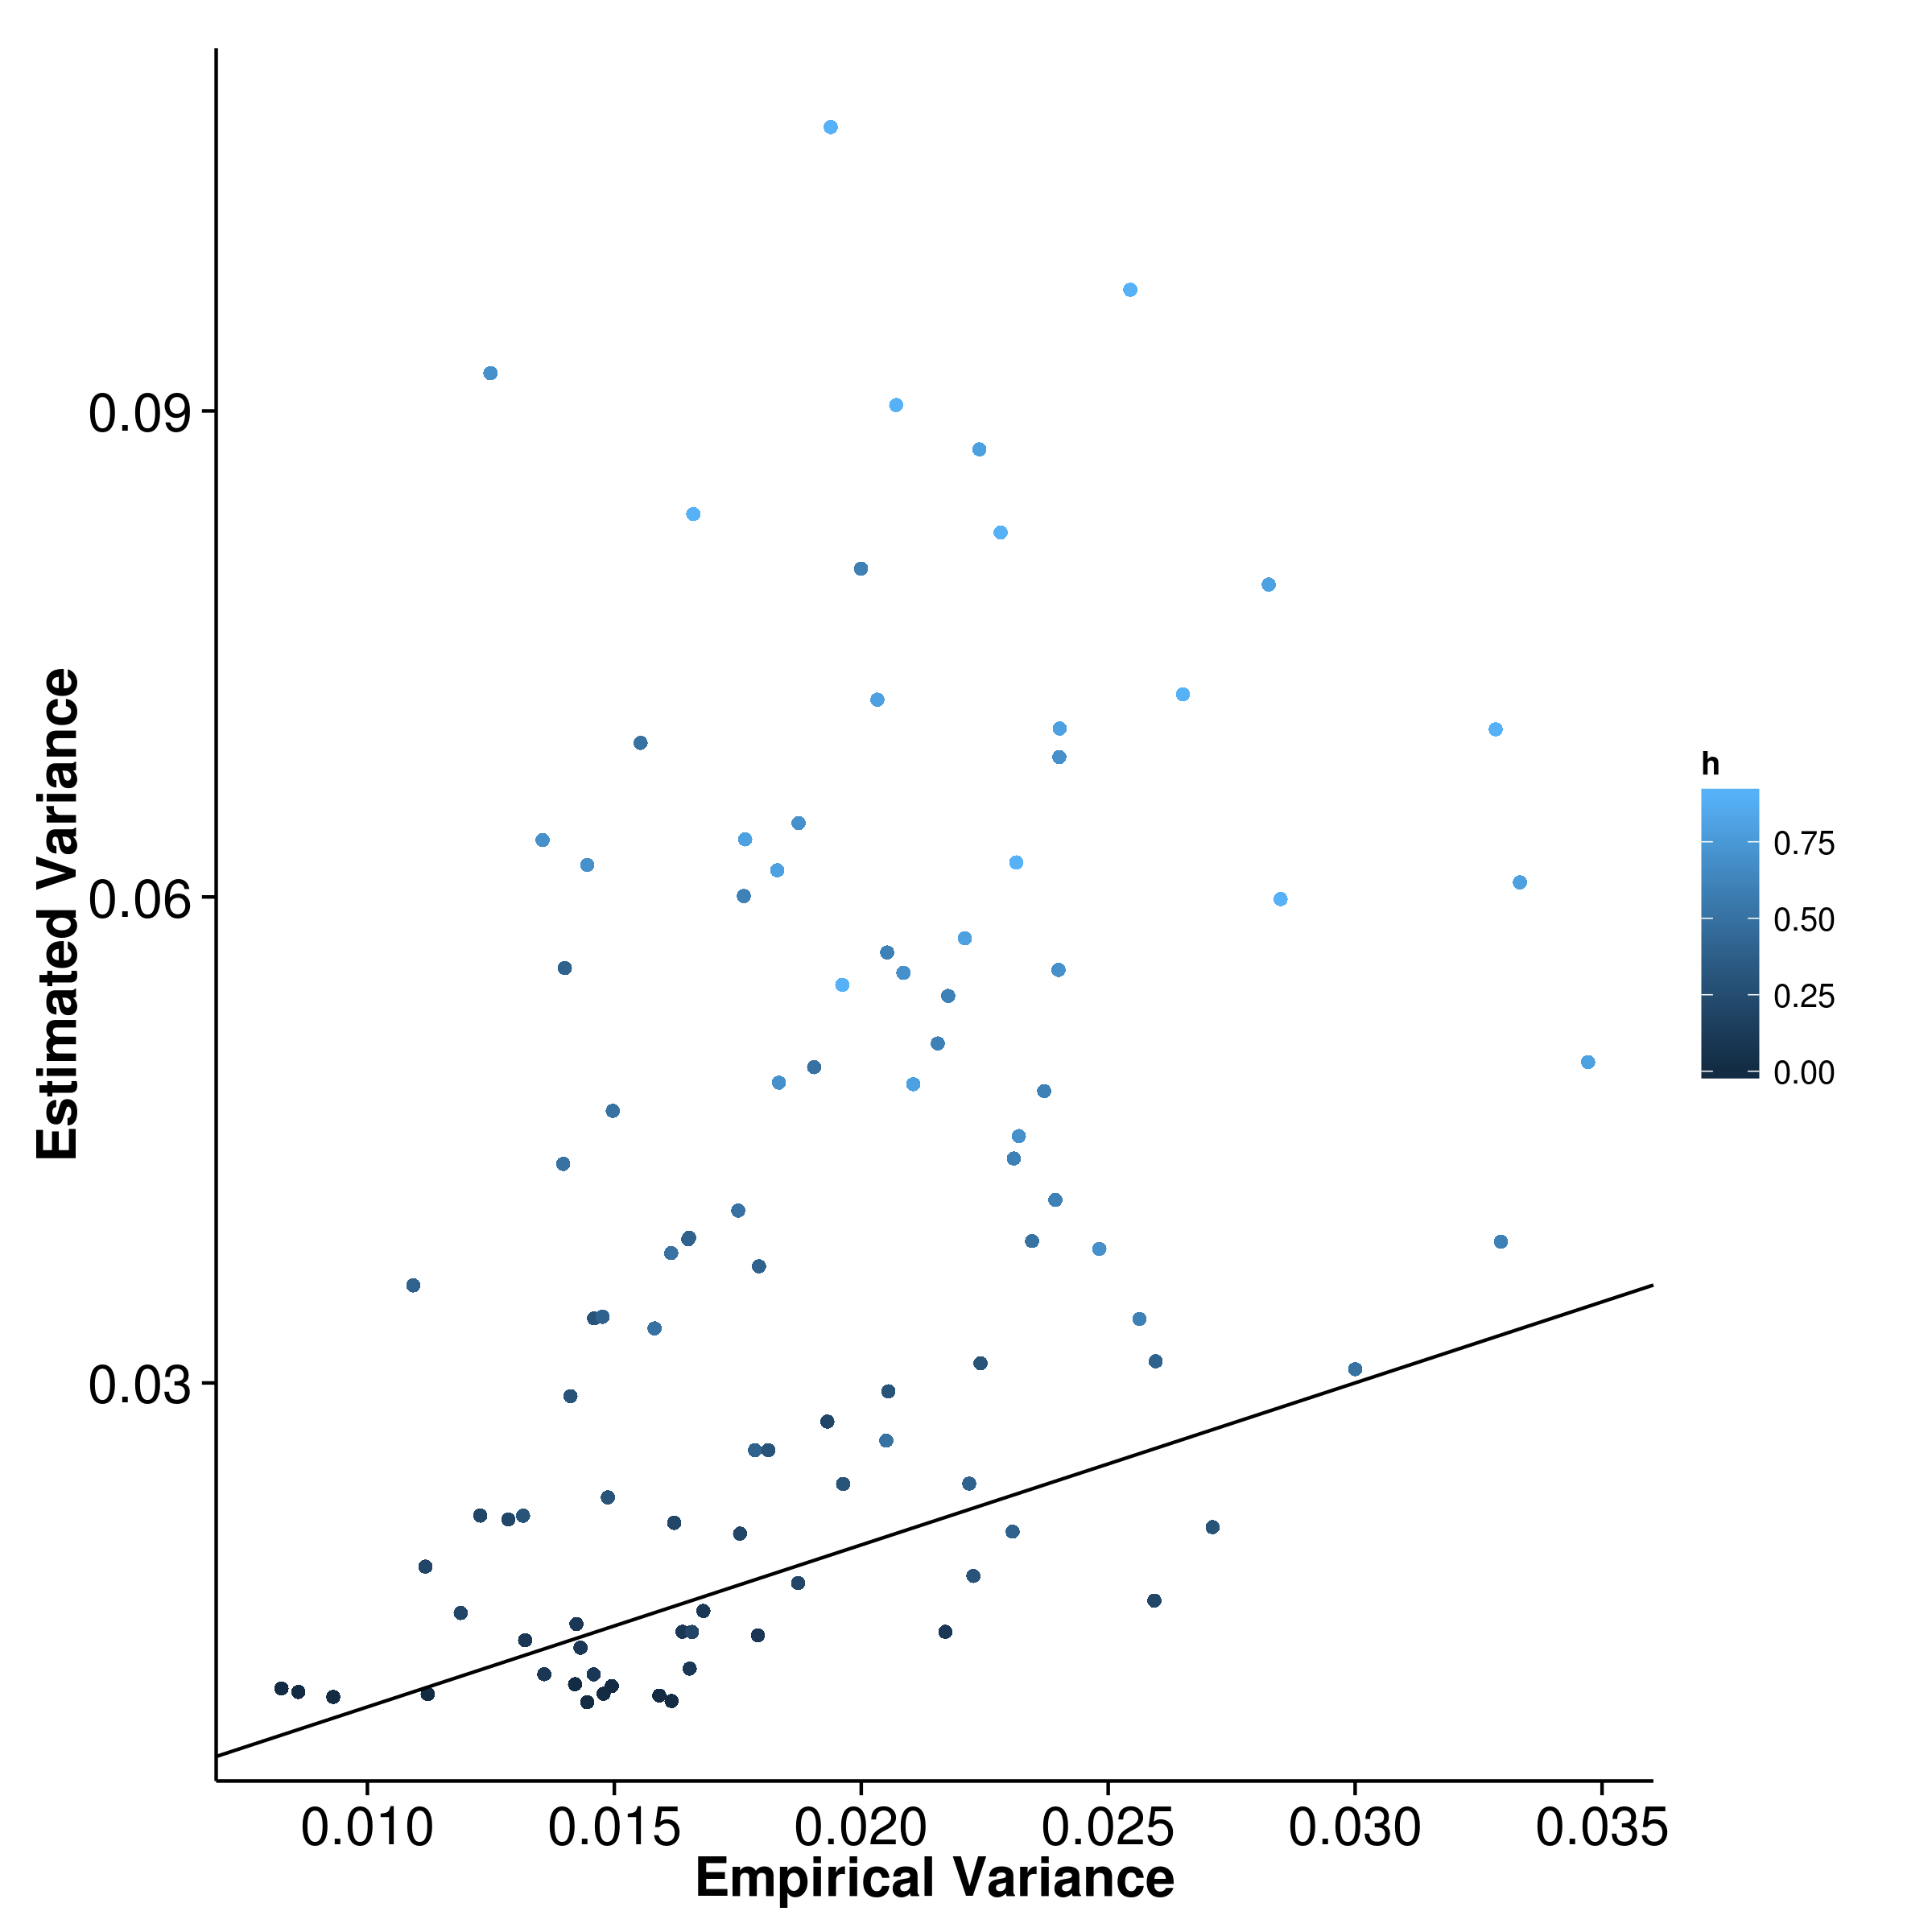
\includegraphics{figure/quantitative/same_effect/50c/ldscIn_50k_50c_varH.png}}
			\label{fig:50k50cQtvarI}
		}
		\label{fig:50k50cQtVar}
	\end{figure}
	
	
	\begin{figure}
		\centering
		\subfloat[SHREK]{
			\scalebox{.4}{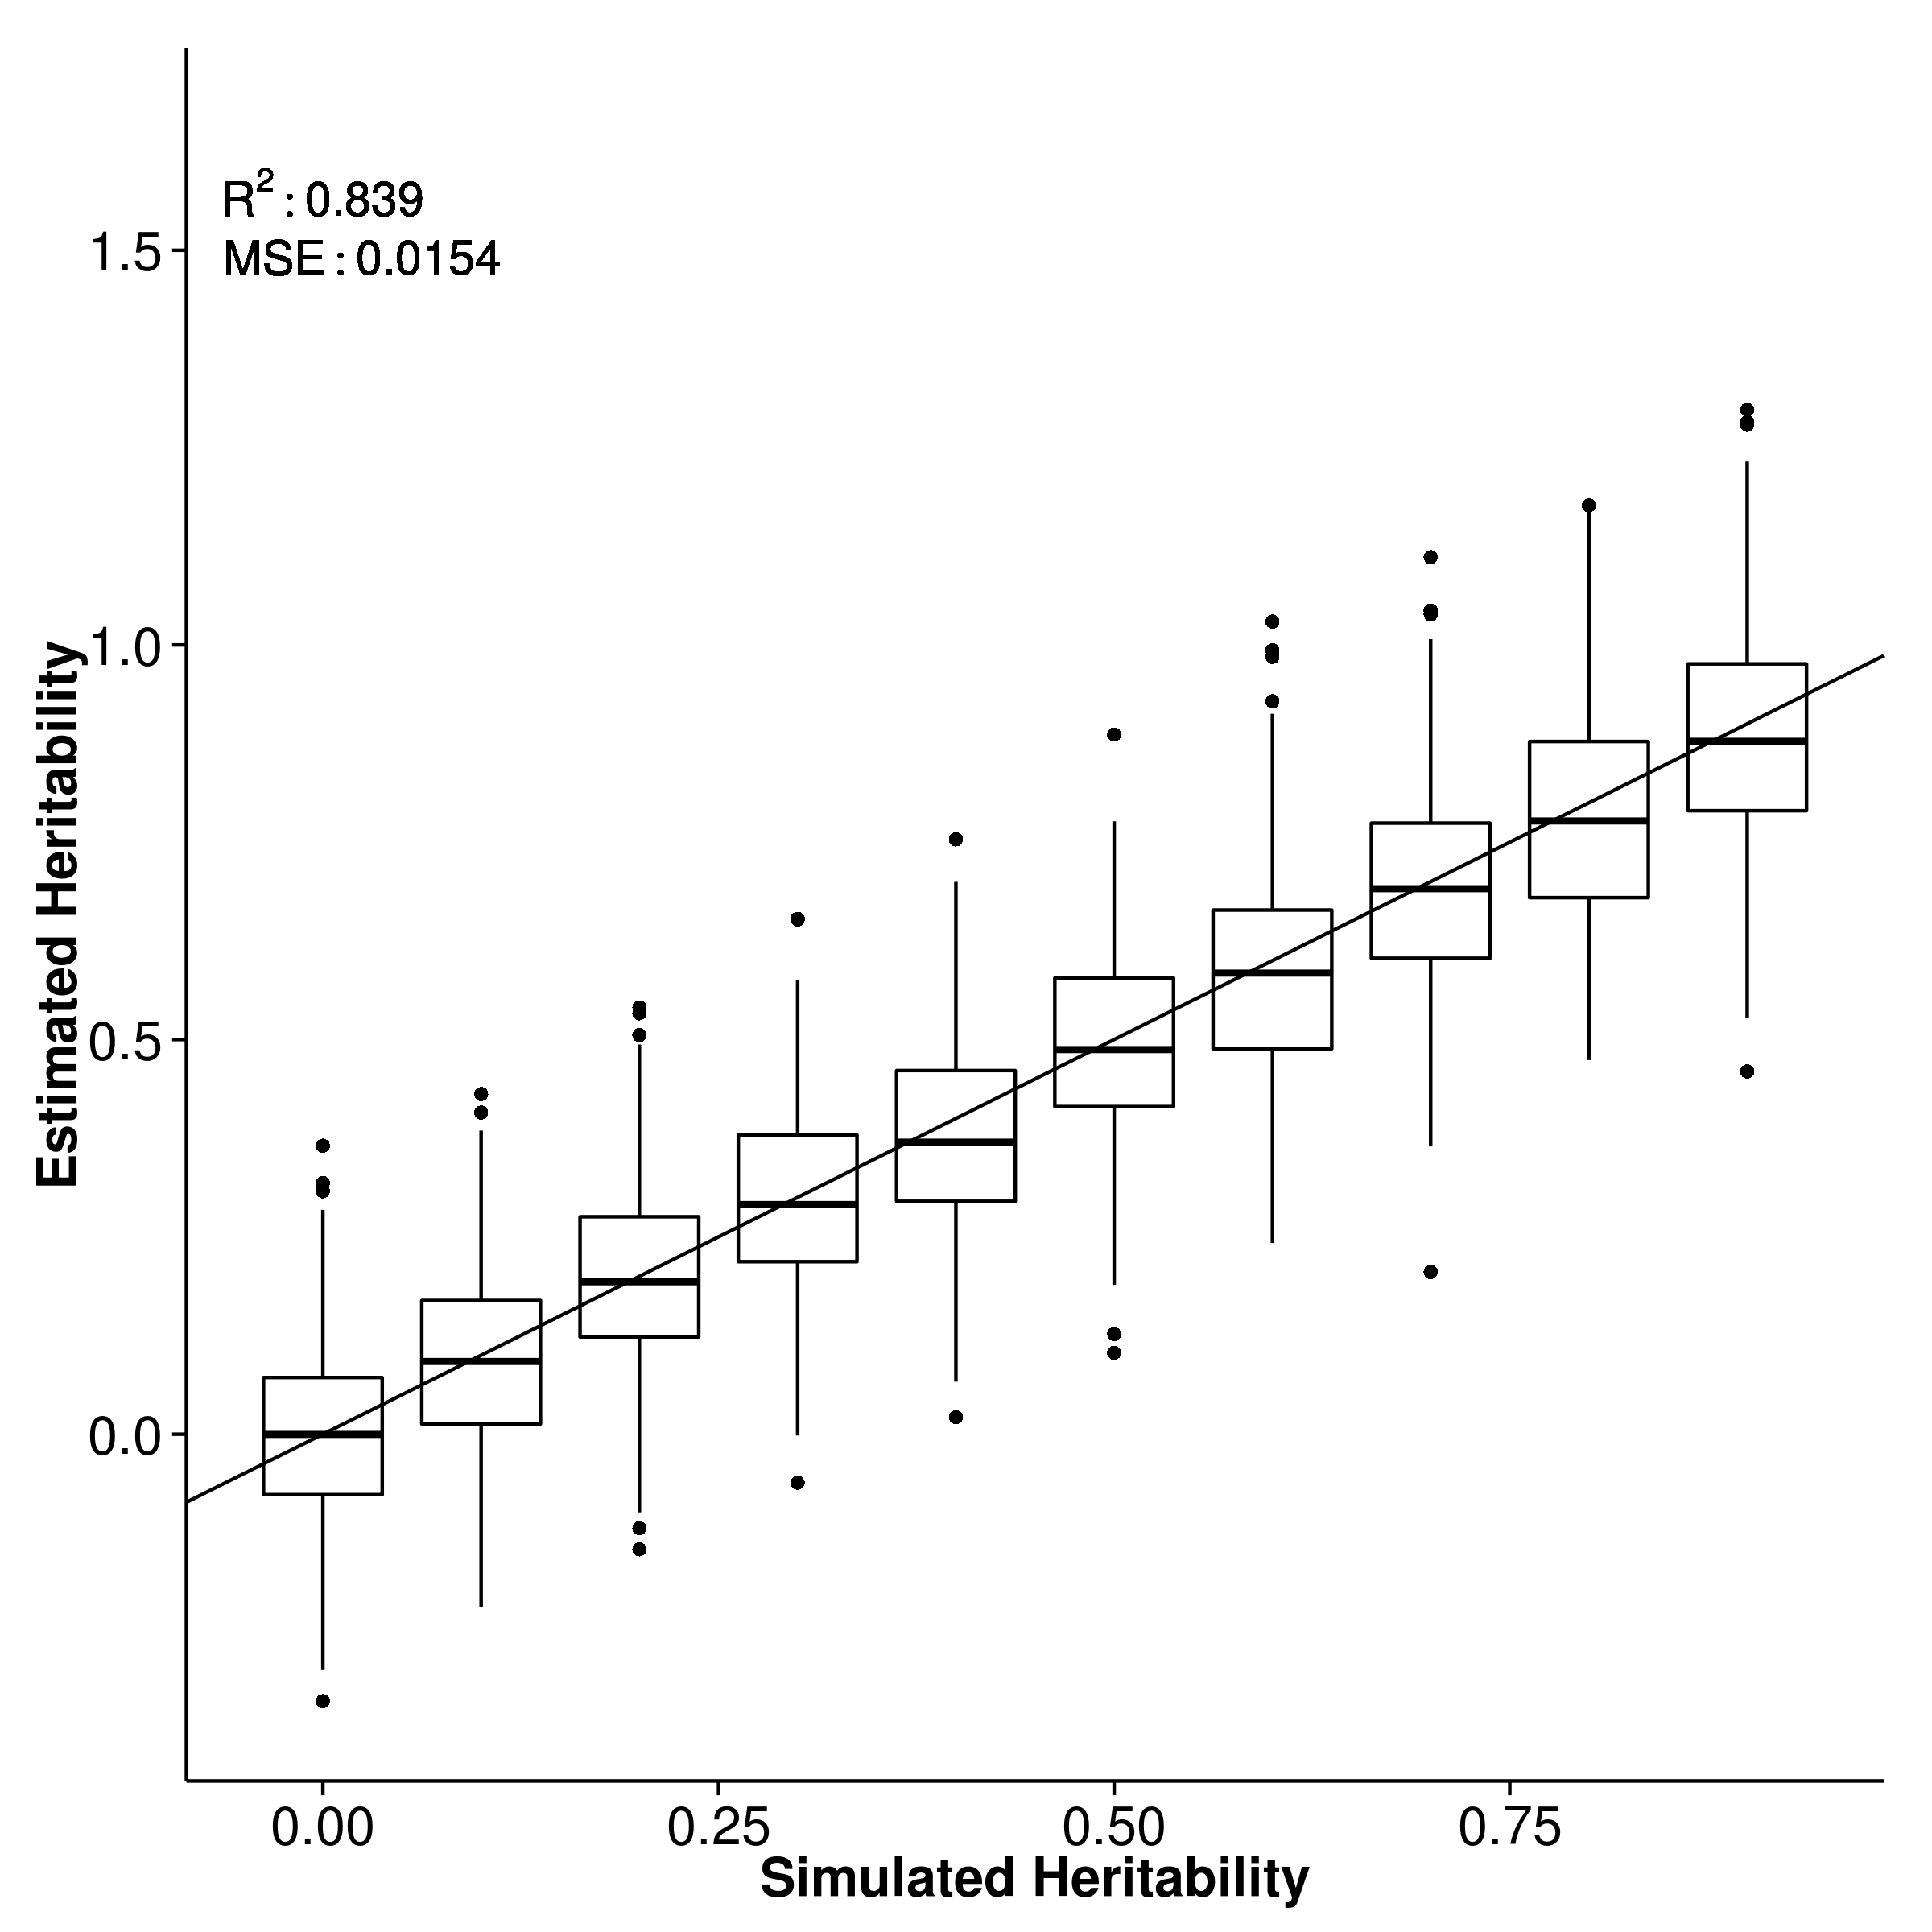
\includegraphics{figure/quantitative/same_effect/100c/shrek_50k_100c_meanH.png}}
			\label{fig:50k100cQtmeanS}
		}
		\subfloat[GCTA]{
			\scalebox{.4}{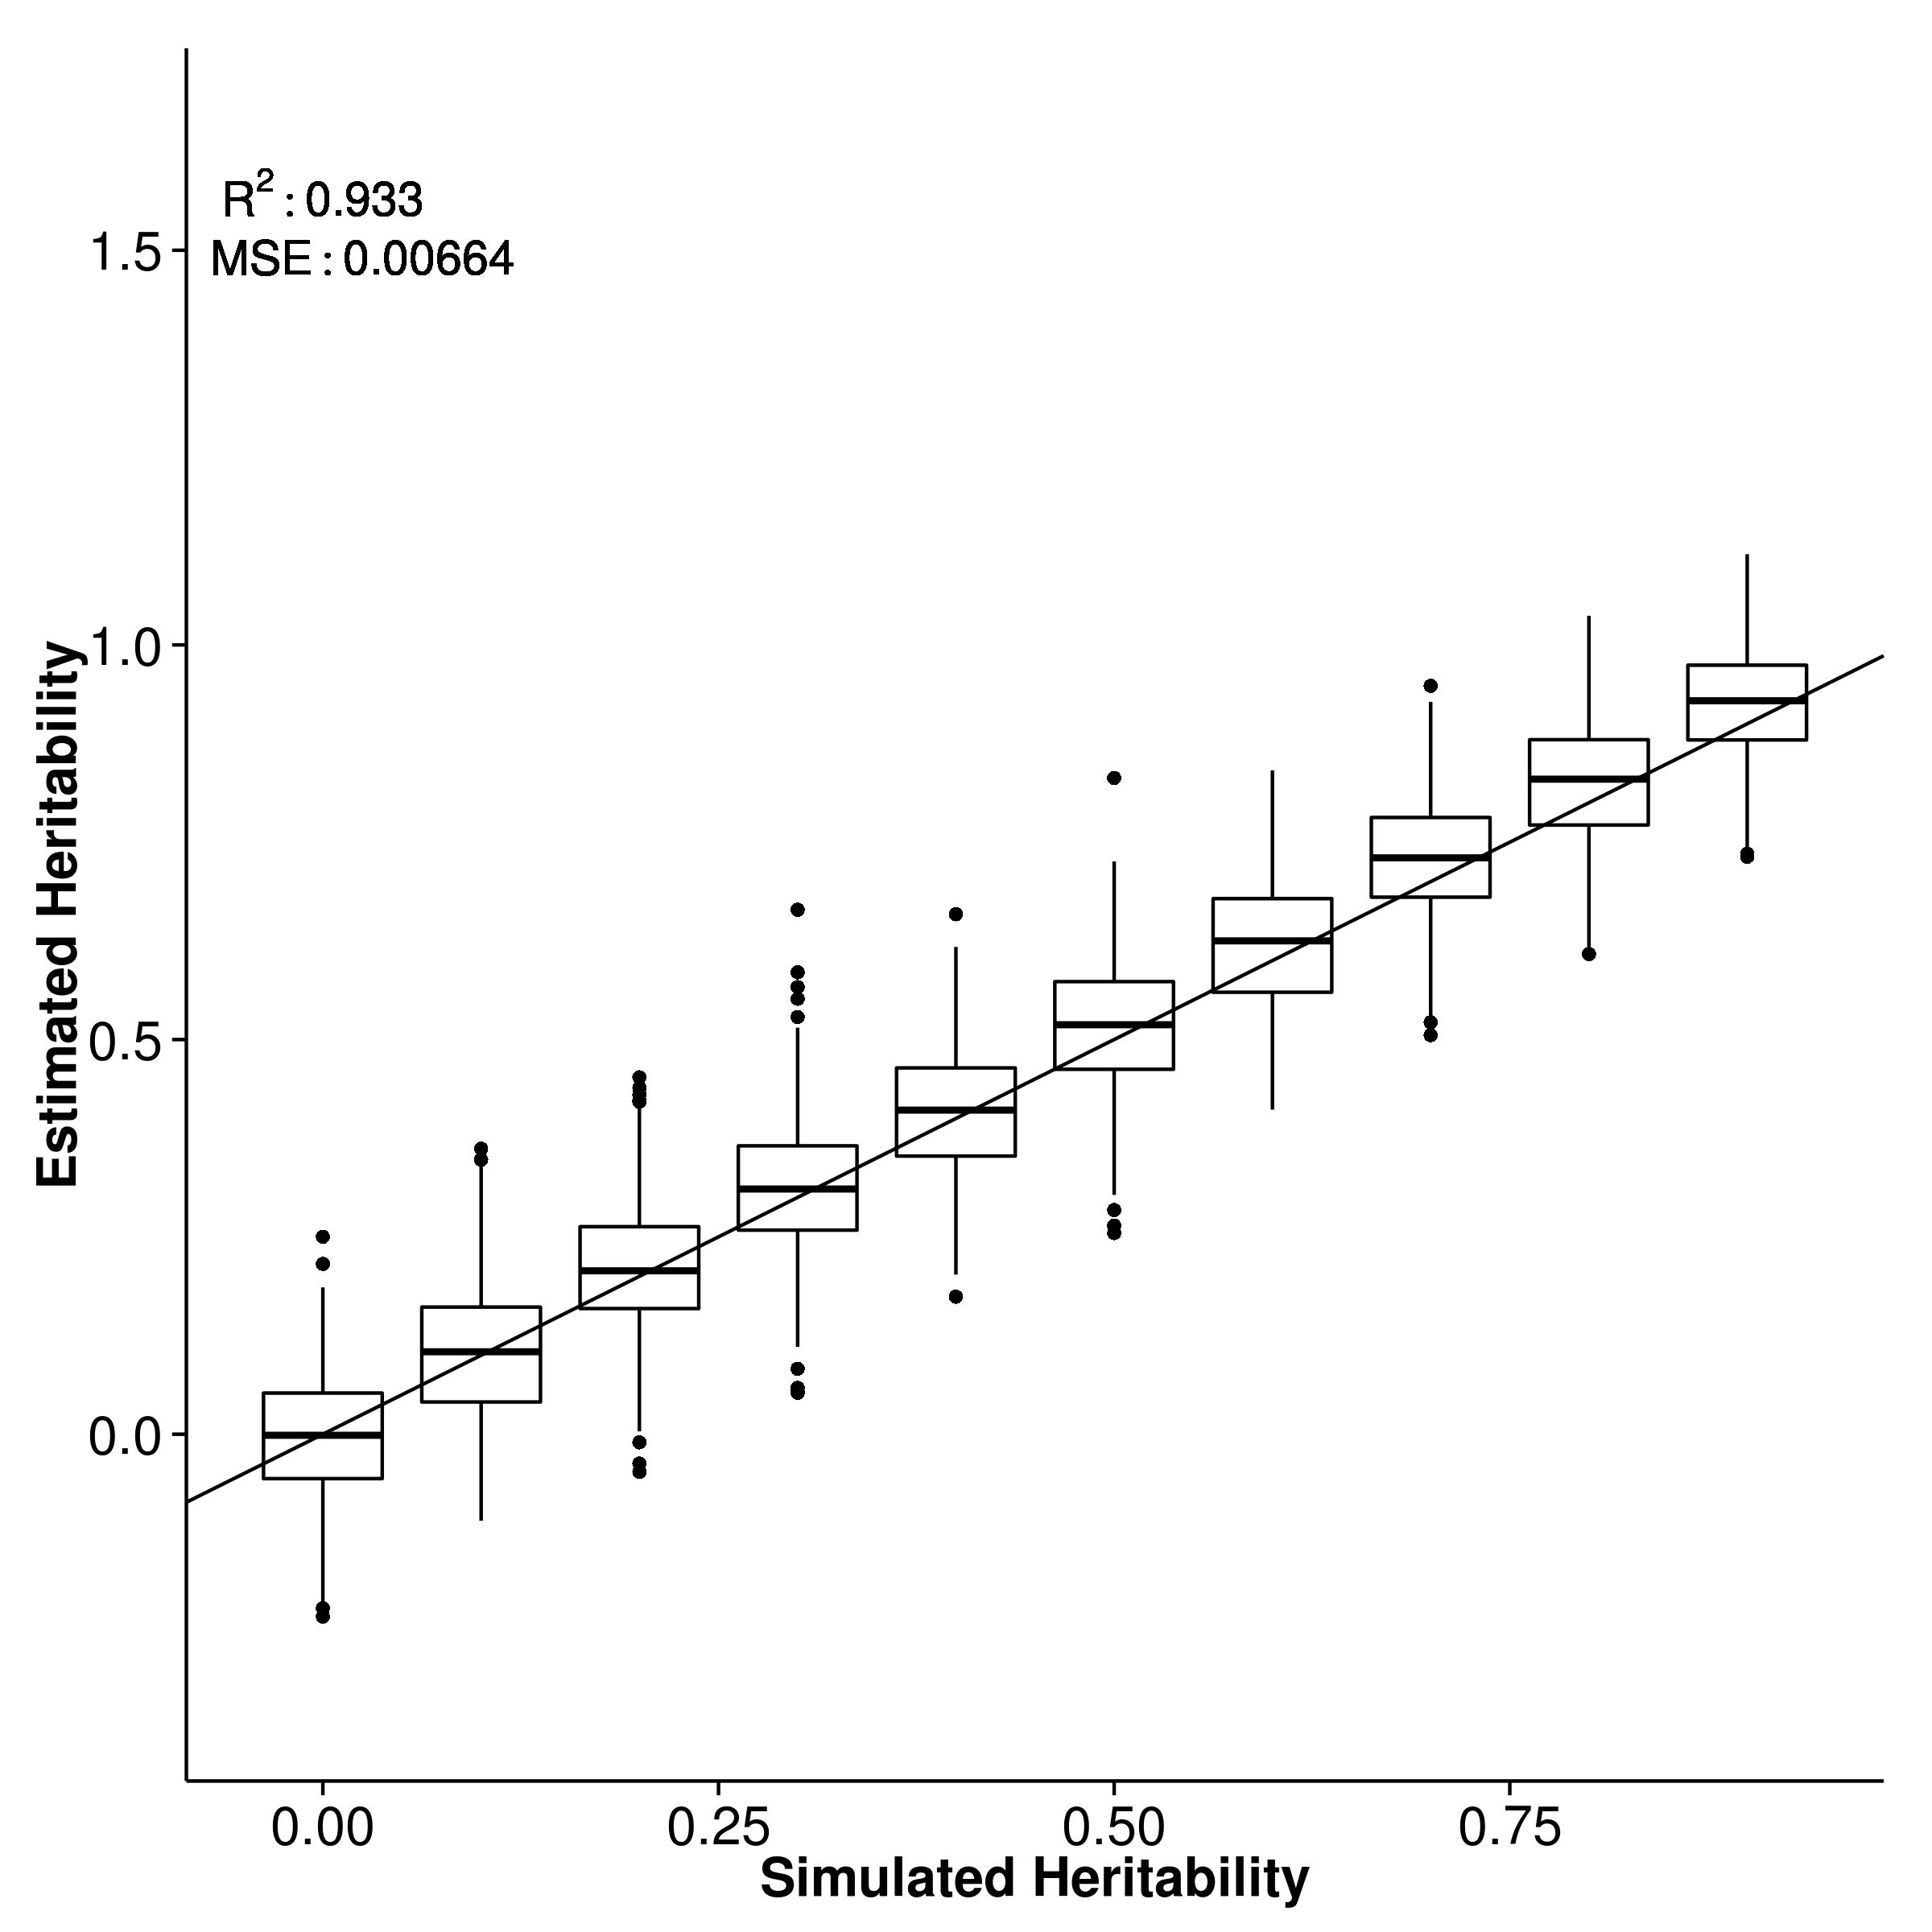
\includegraphics{figure/quantitative/same_effect/100c/gcta_50k_100c_meanH.png}}
			\label{fig:50k100cQtmeanG}
		}\\
		\subfloat[LDSC with fix intercept]{
			\scalebox{.4}{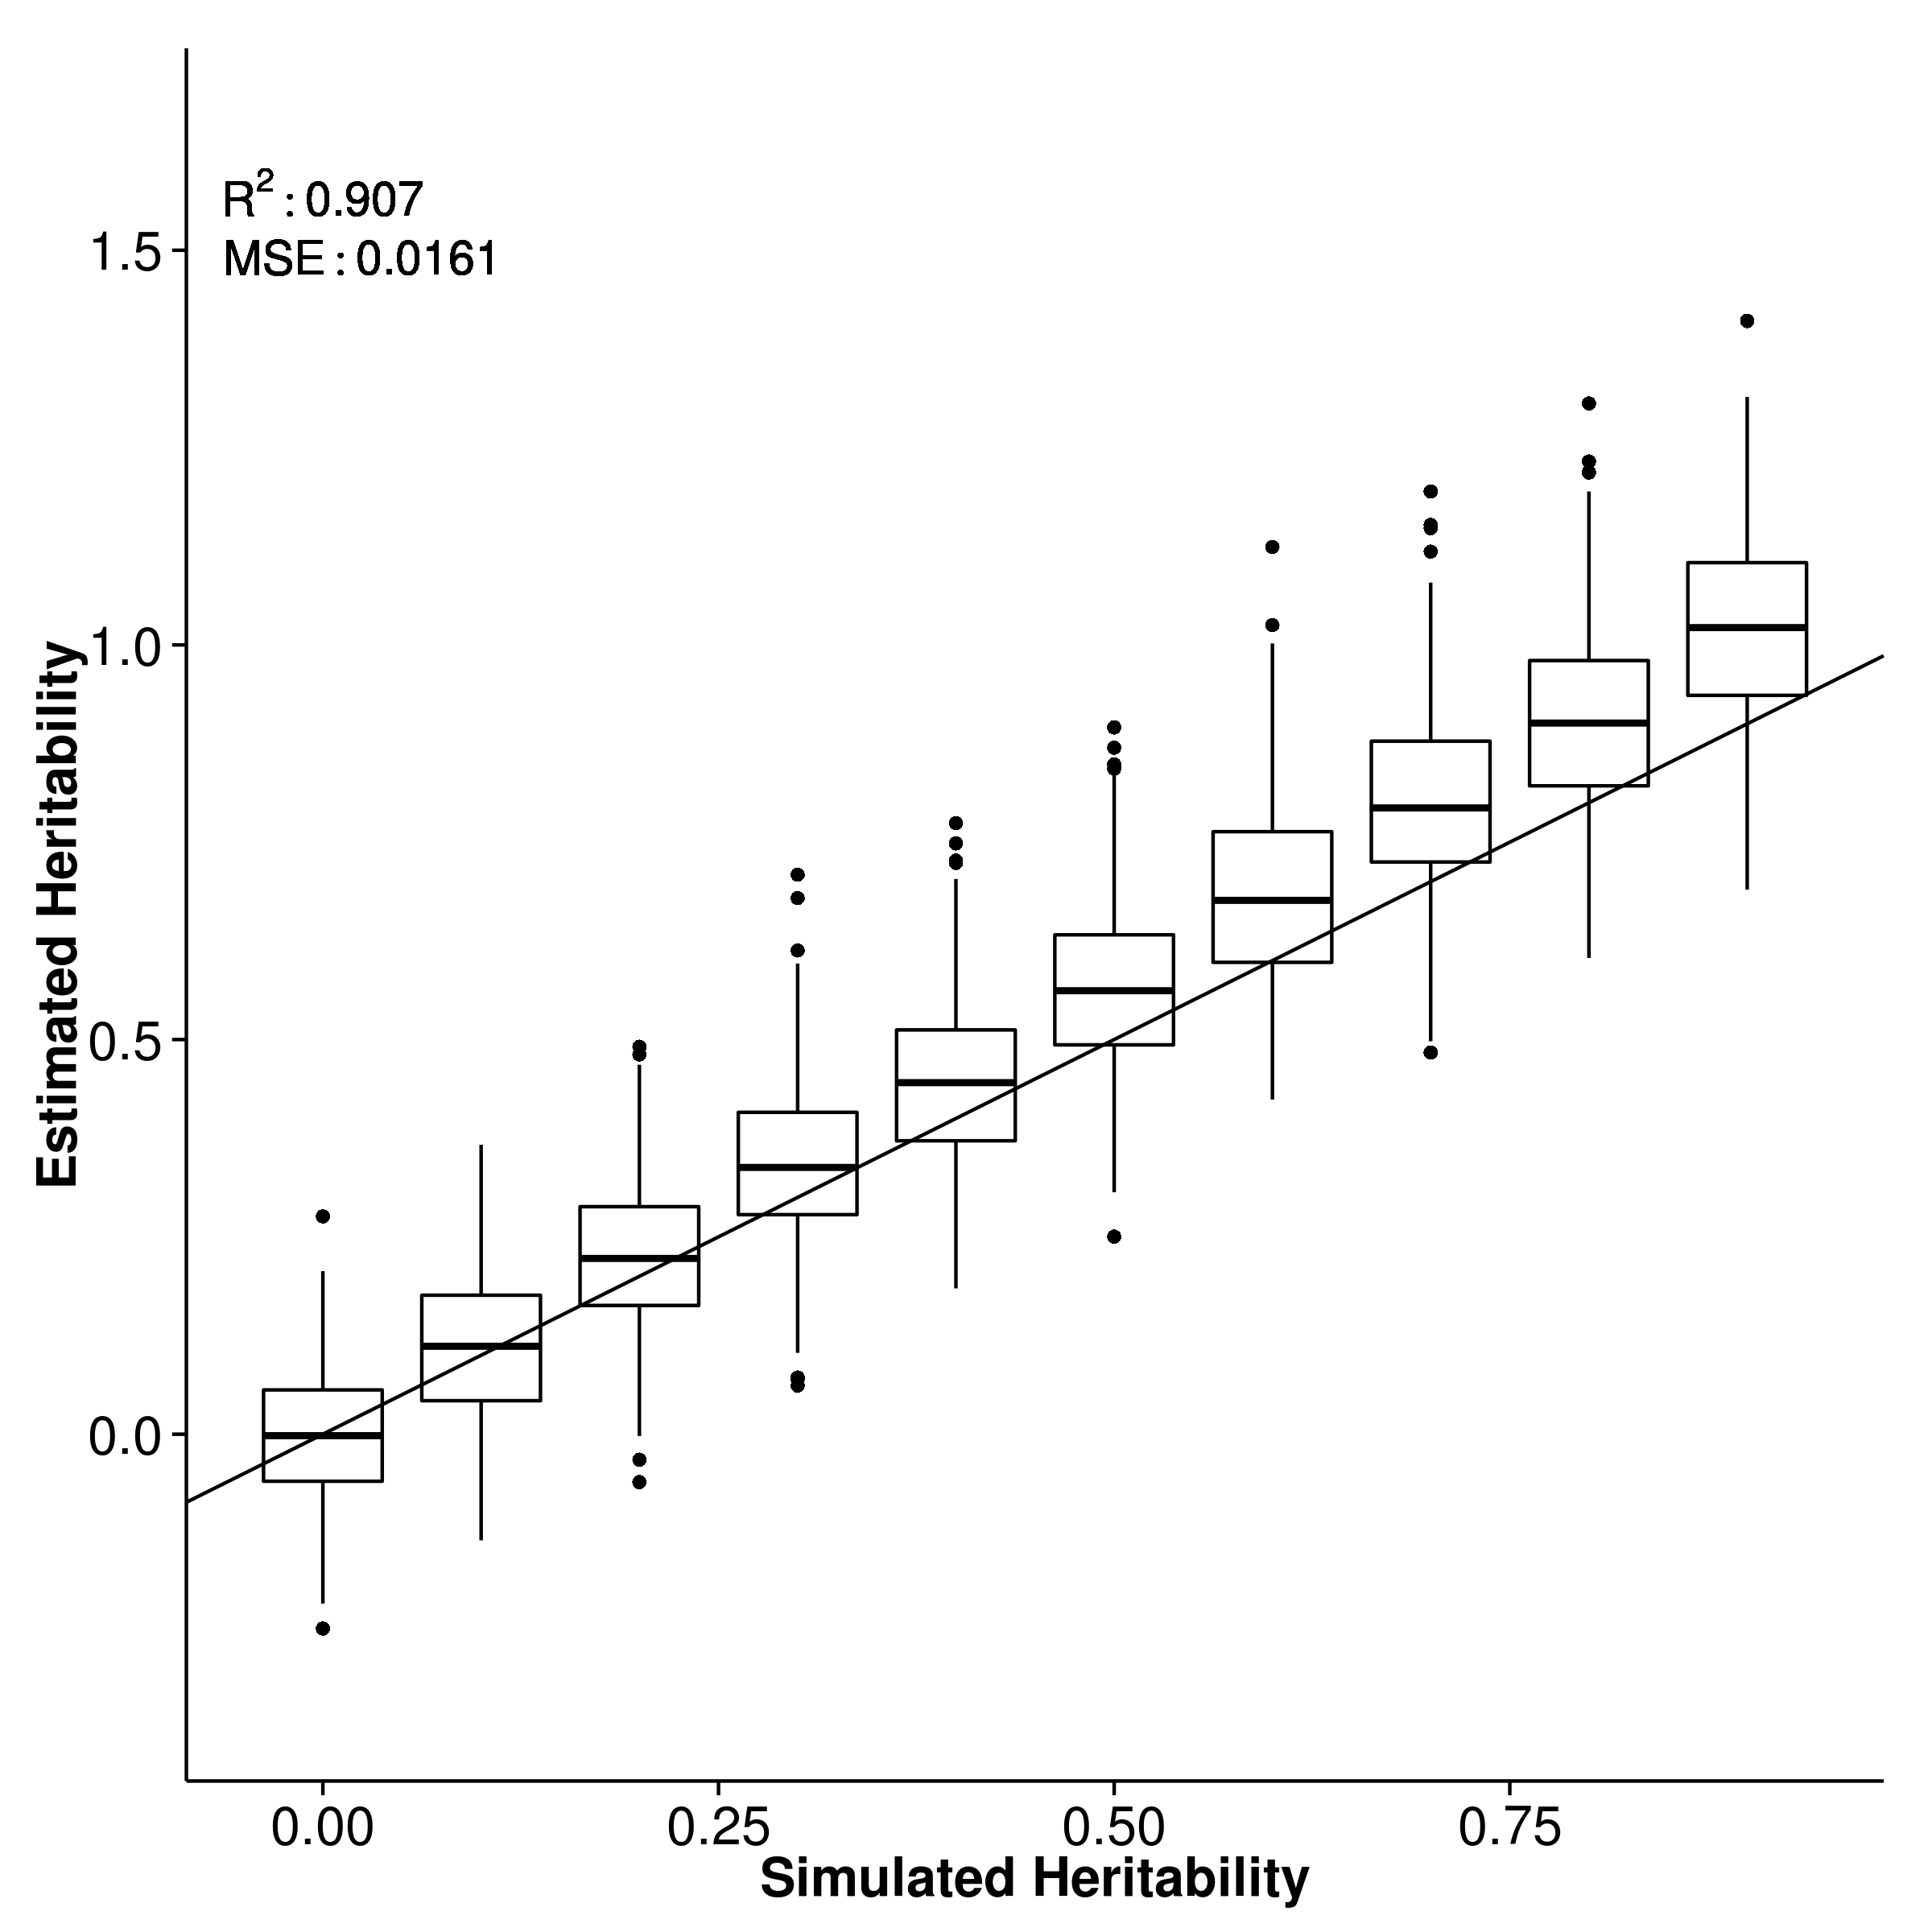
\includegraphics{figure/quantitative/same_effect/100c/ldsc_50k_100c_meanH.png}}
			\label{fig:50k100cQtmeanL}
		}
		\subfloat[LDSC with intercept estimation]{
			\scalebox{.4}{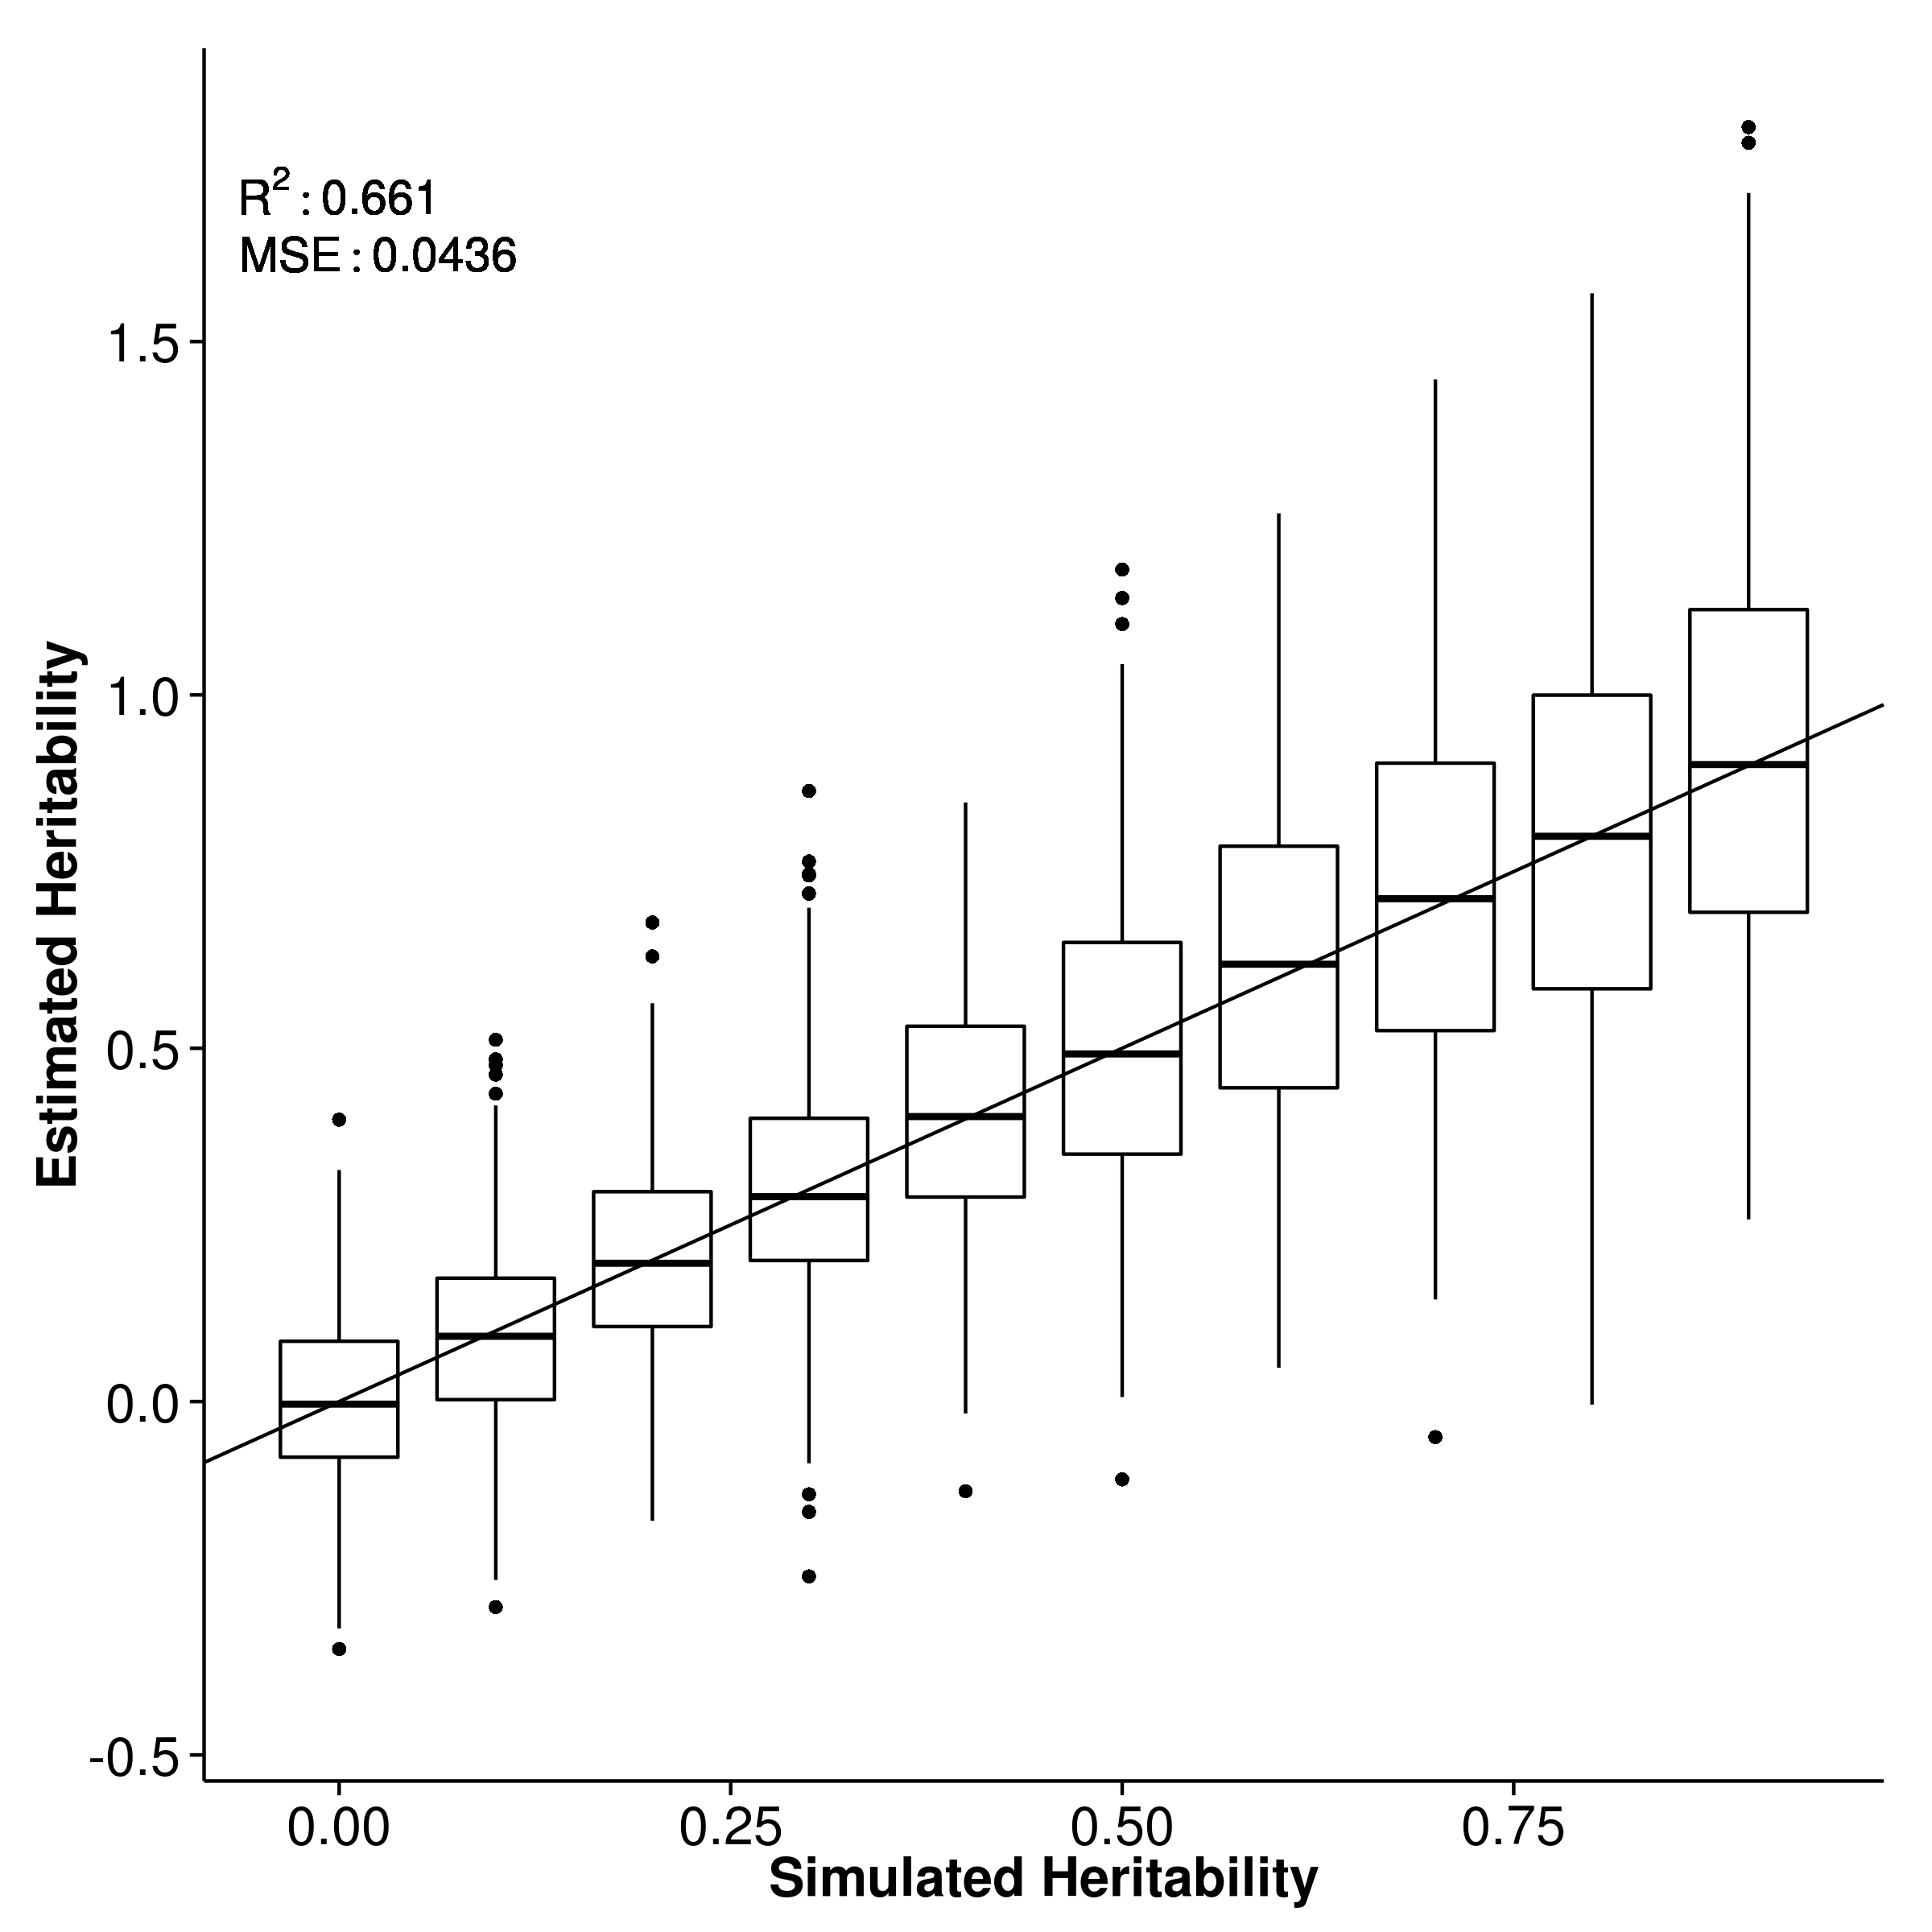
\includegraphics{figure/quantitative/same_effect/100c/ldscIn_50k_100c_meanH.png}}
			\label{fig:50k100cQtmeanI}
		}
		\caption[Simulation of Quantitative Traits with 50k \glsentryshortpl{SNP} and 100 causal variants of same effect size]
		{Simulation of Quantitative Traits with 50k \glsentryshortpl{SNP} and 100 causal variants with same effect size.} 
		\label{fig:50k100cQtMean}
	\end{figure}
	\begin{figure}
		\centering
		\subfloat[SHREK]{
			\scalebox{.4}{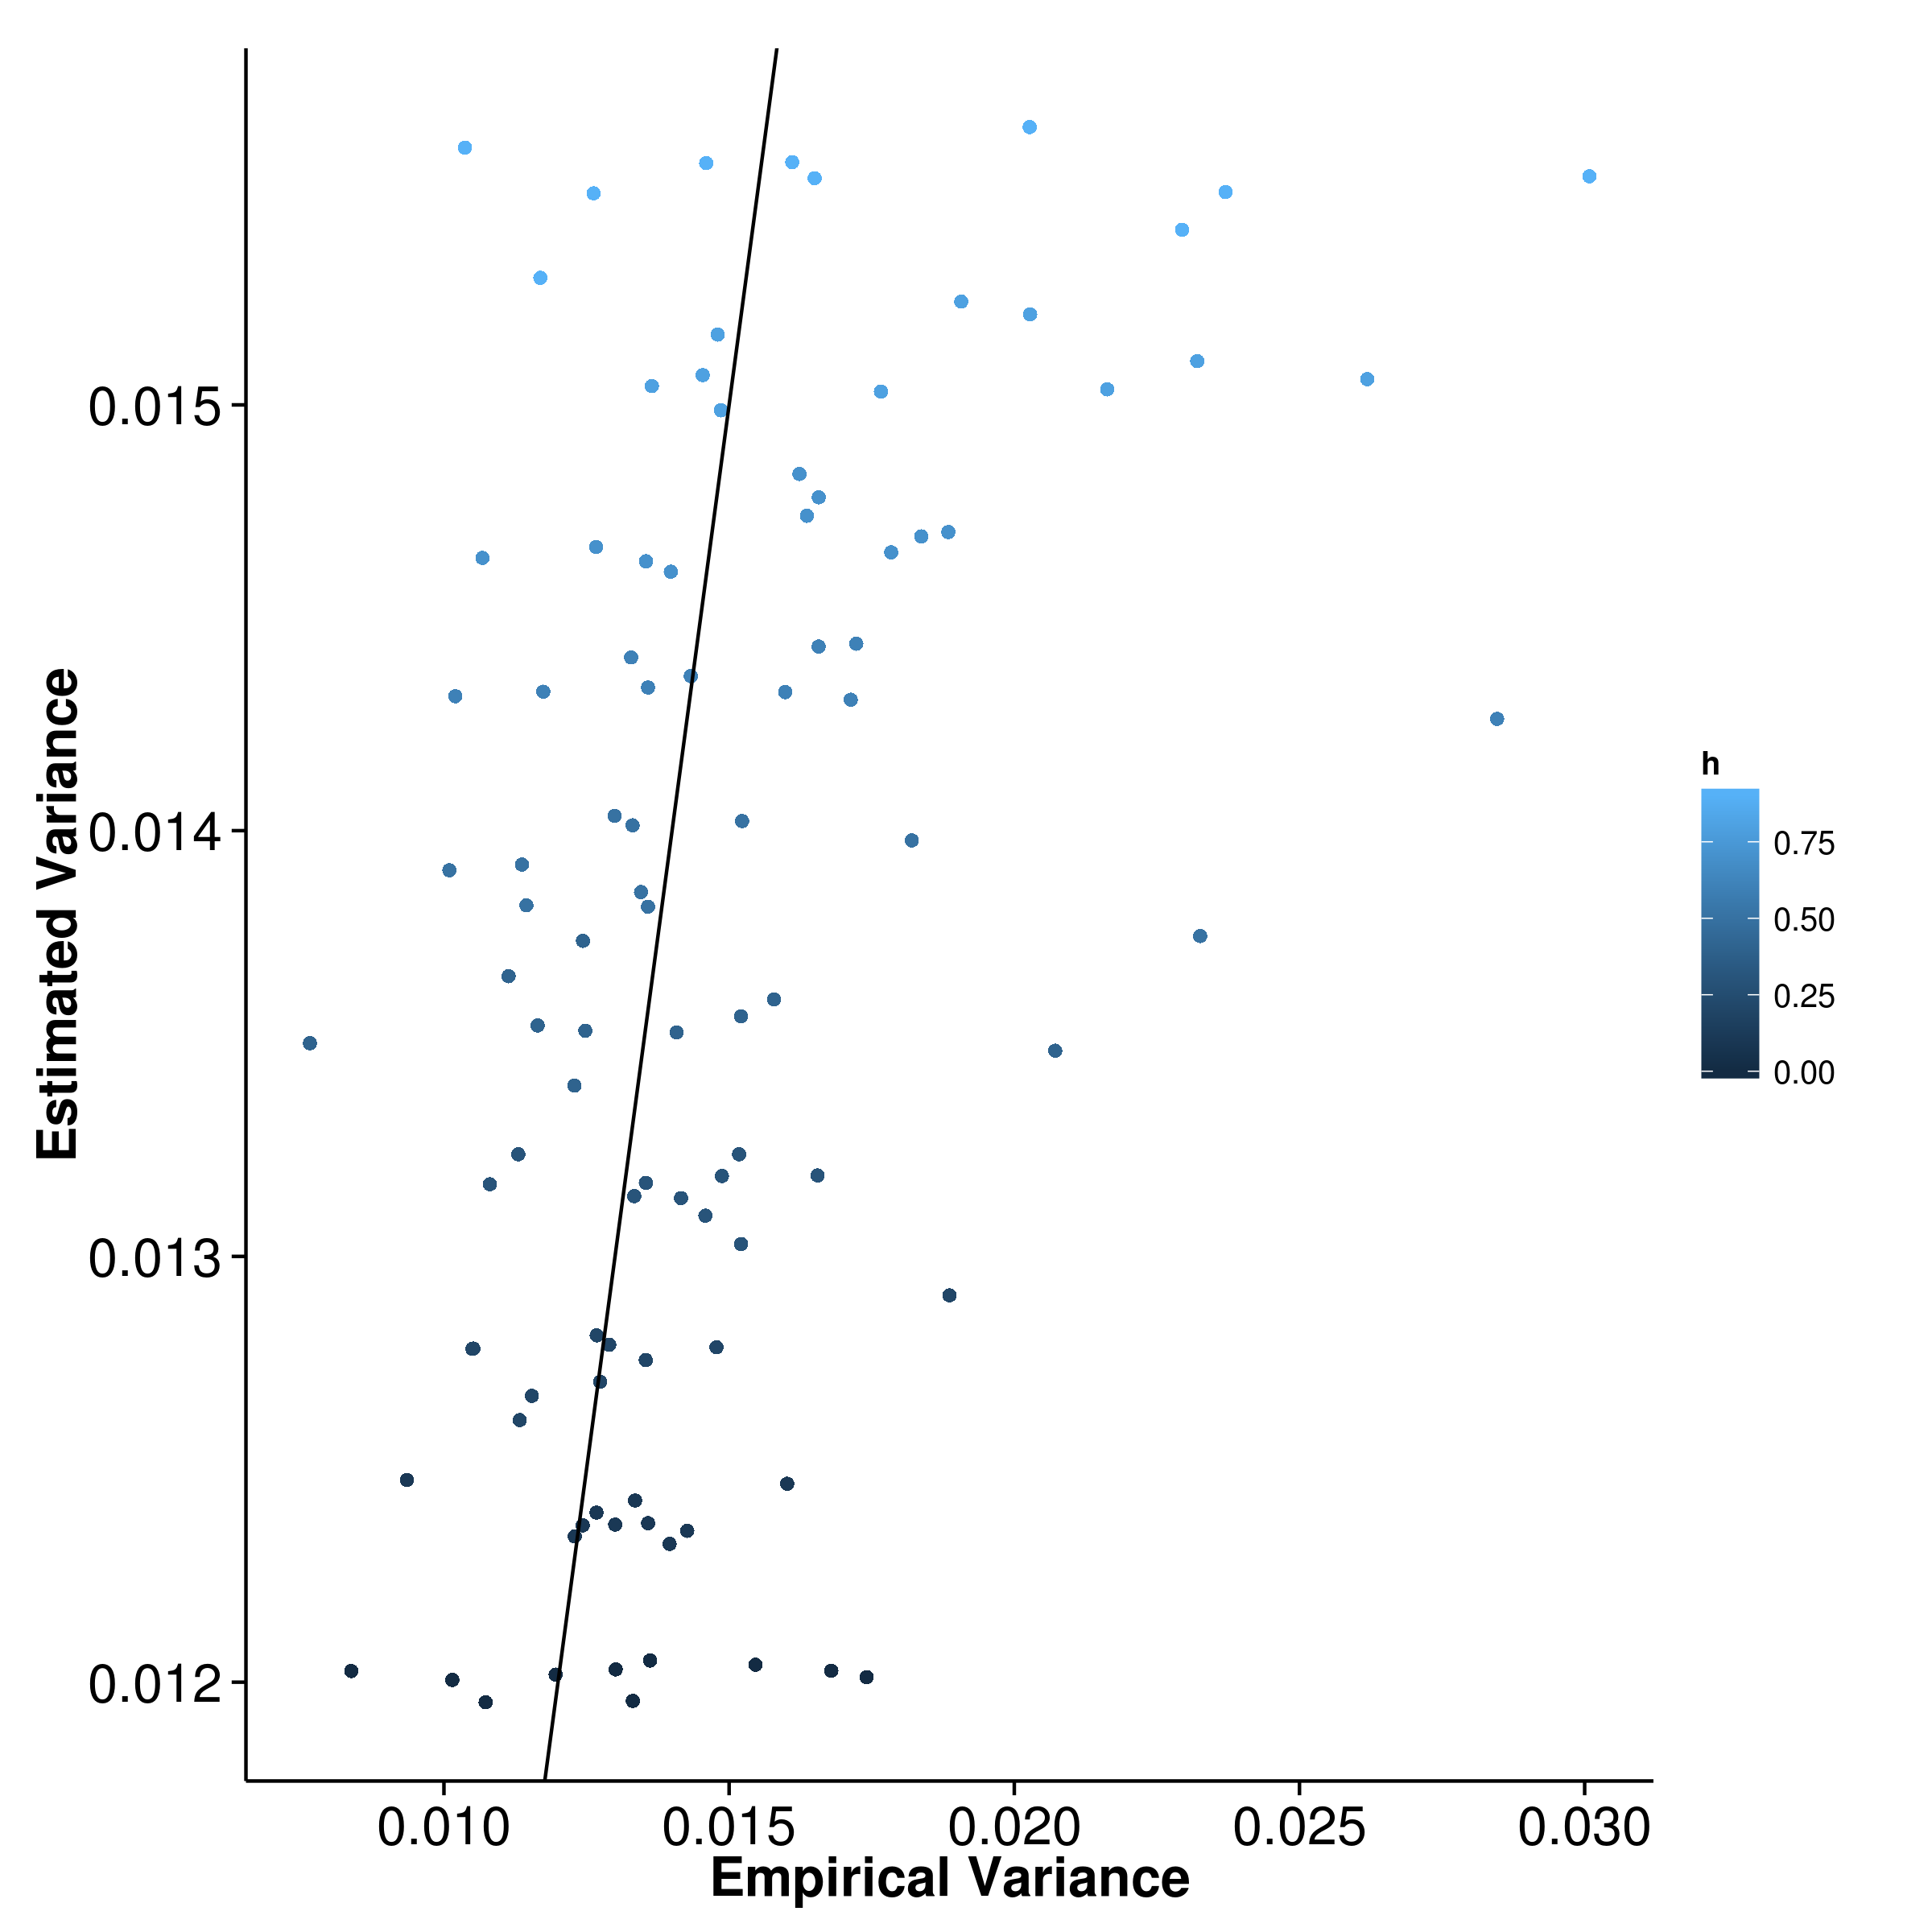
\includegraphics{figure/quantitative/same_effect/100c/shrek_50k_100c_varH.png}}
			\label{fig:50k100cQtvarS}
		}
		\subfloat[GCTA]{
			\scalebox{.4}{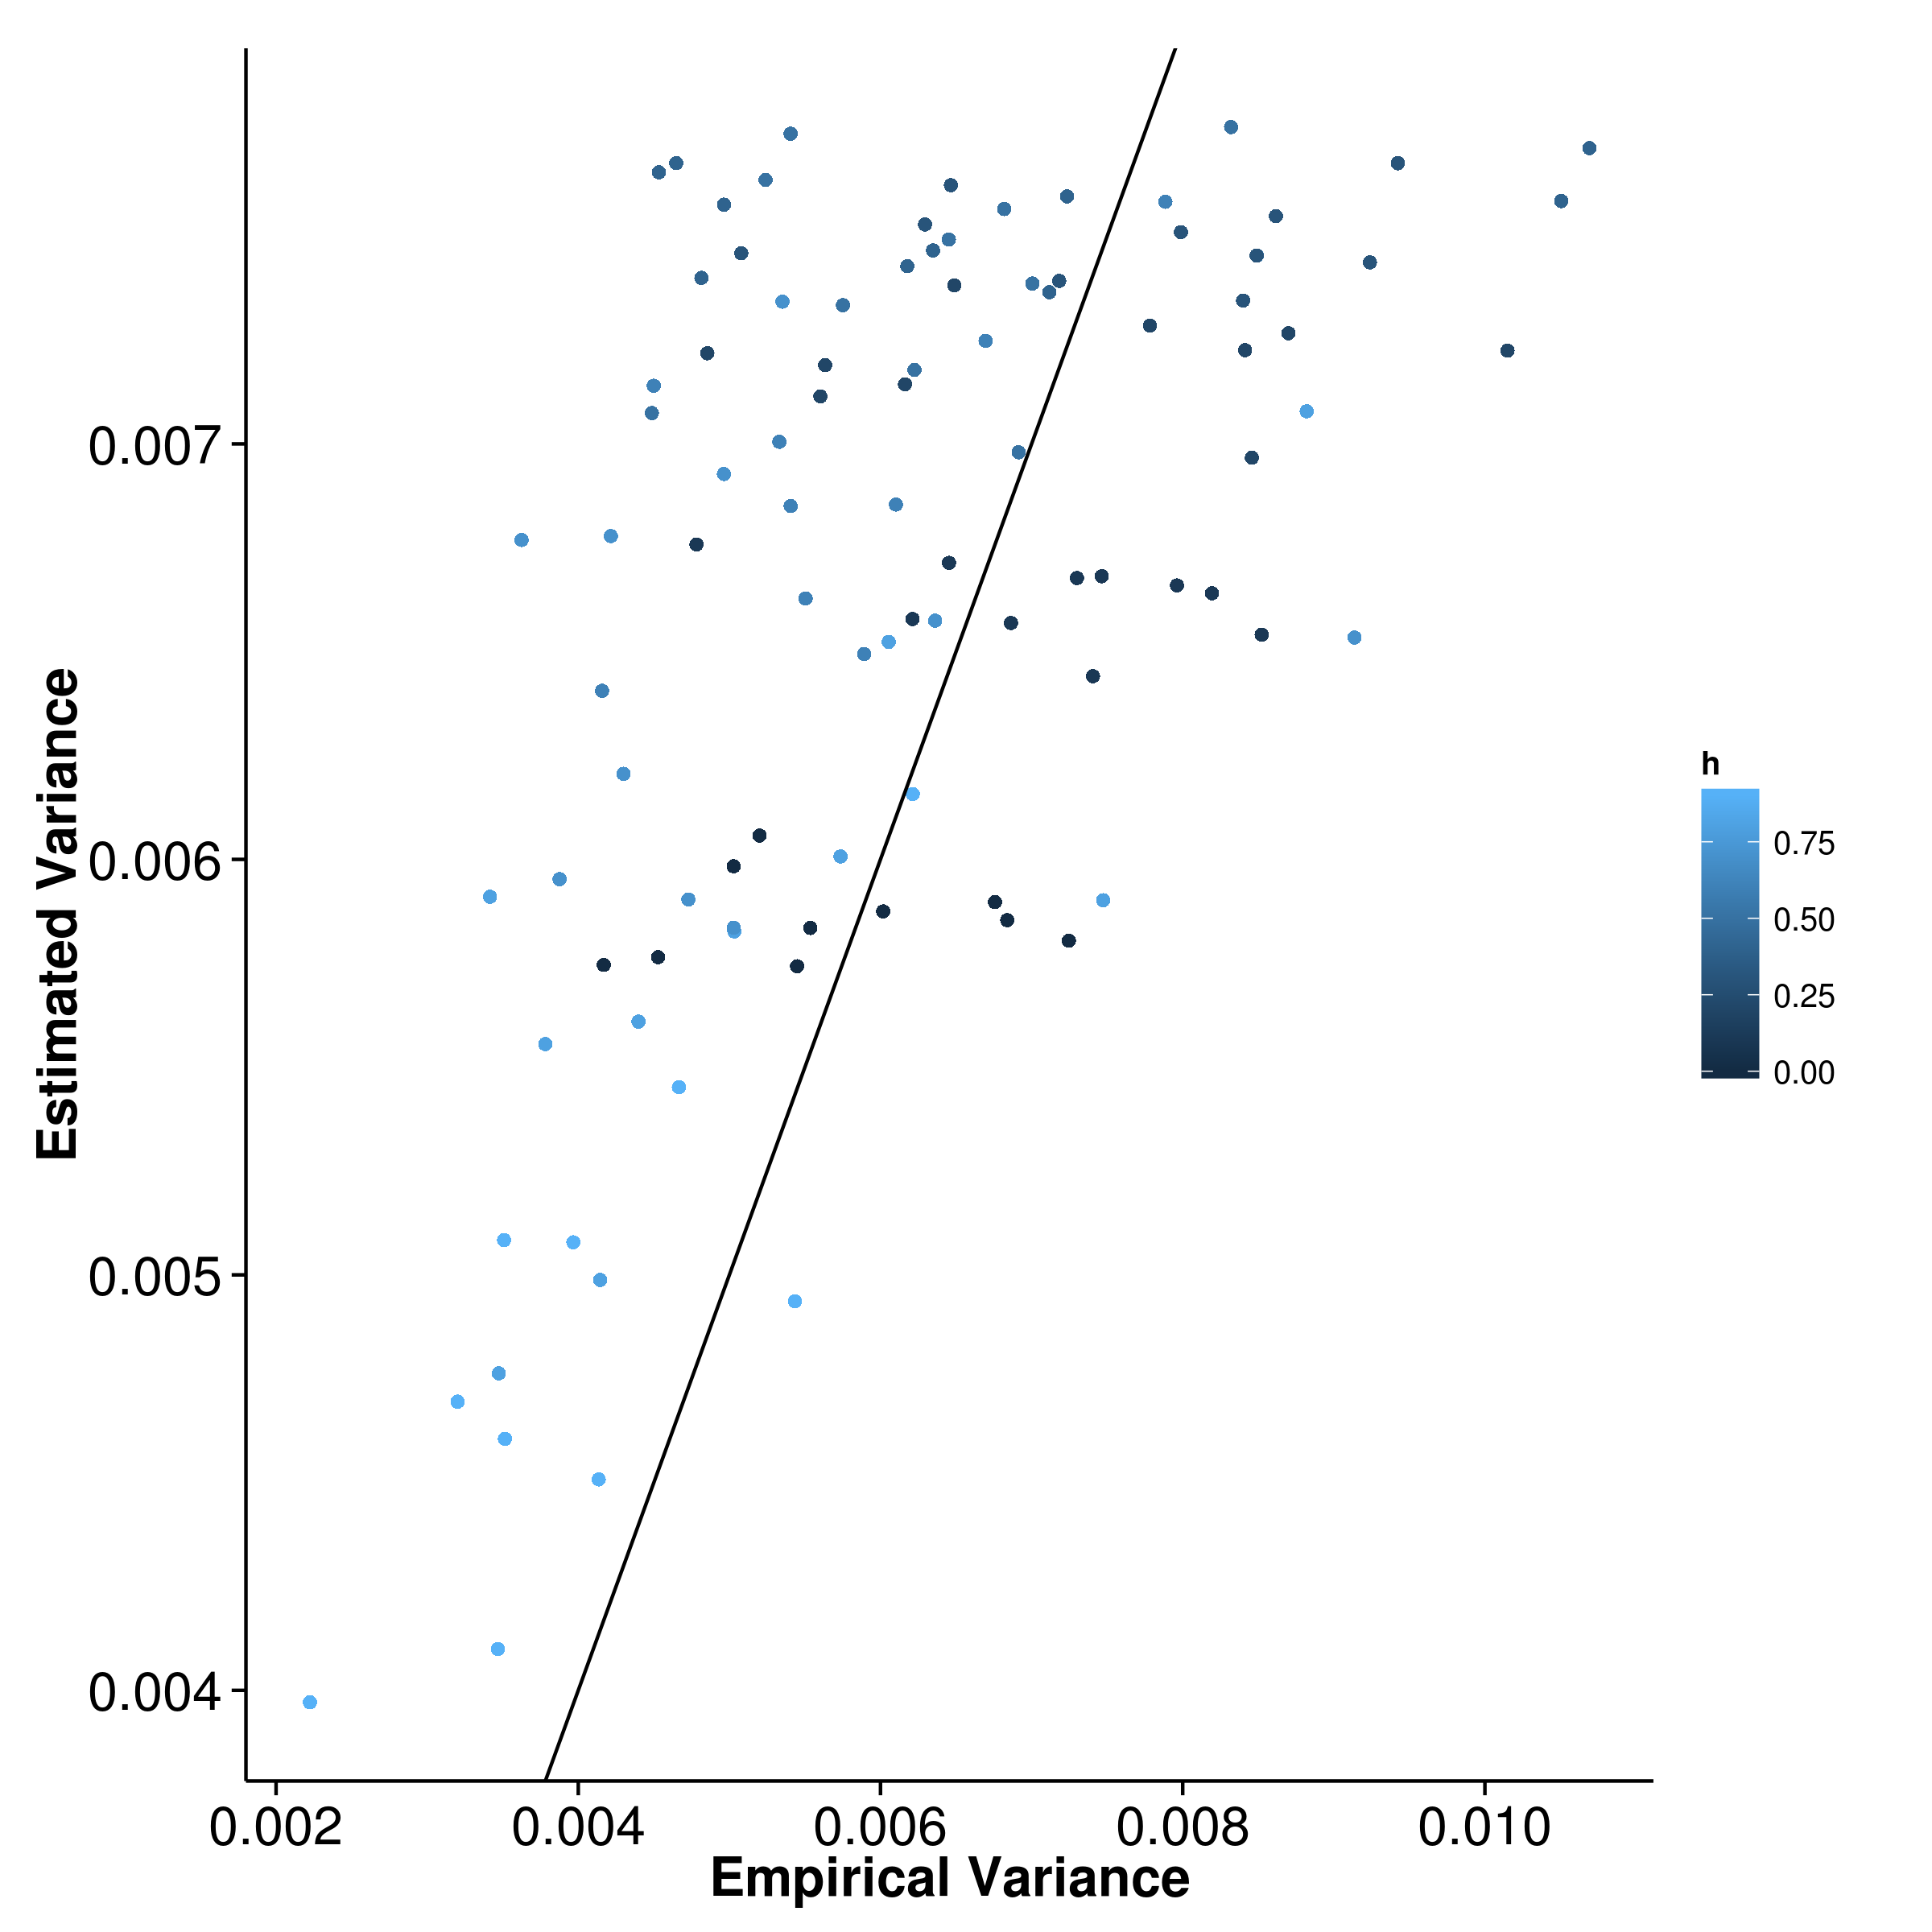
\includegraphics{figure/quantitative/same_effect/100c/gcta_50k_100c_varH.png}}
			\label{fig:50k100cQtvarG}
		}\\
		\subfloat[LDSC with fix intercept]{
			\scalebox{.4}{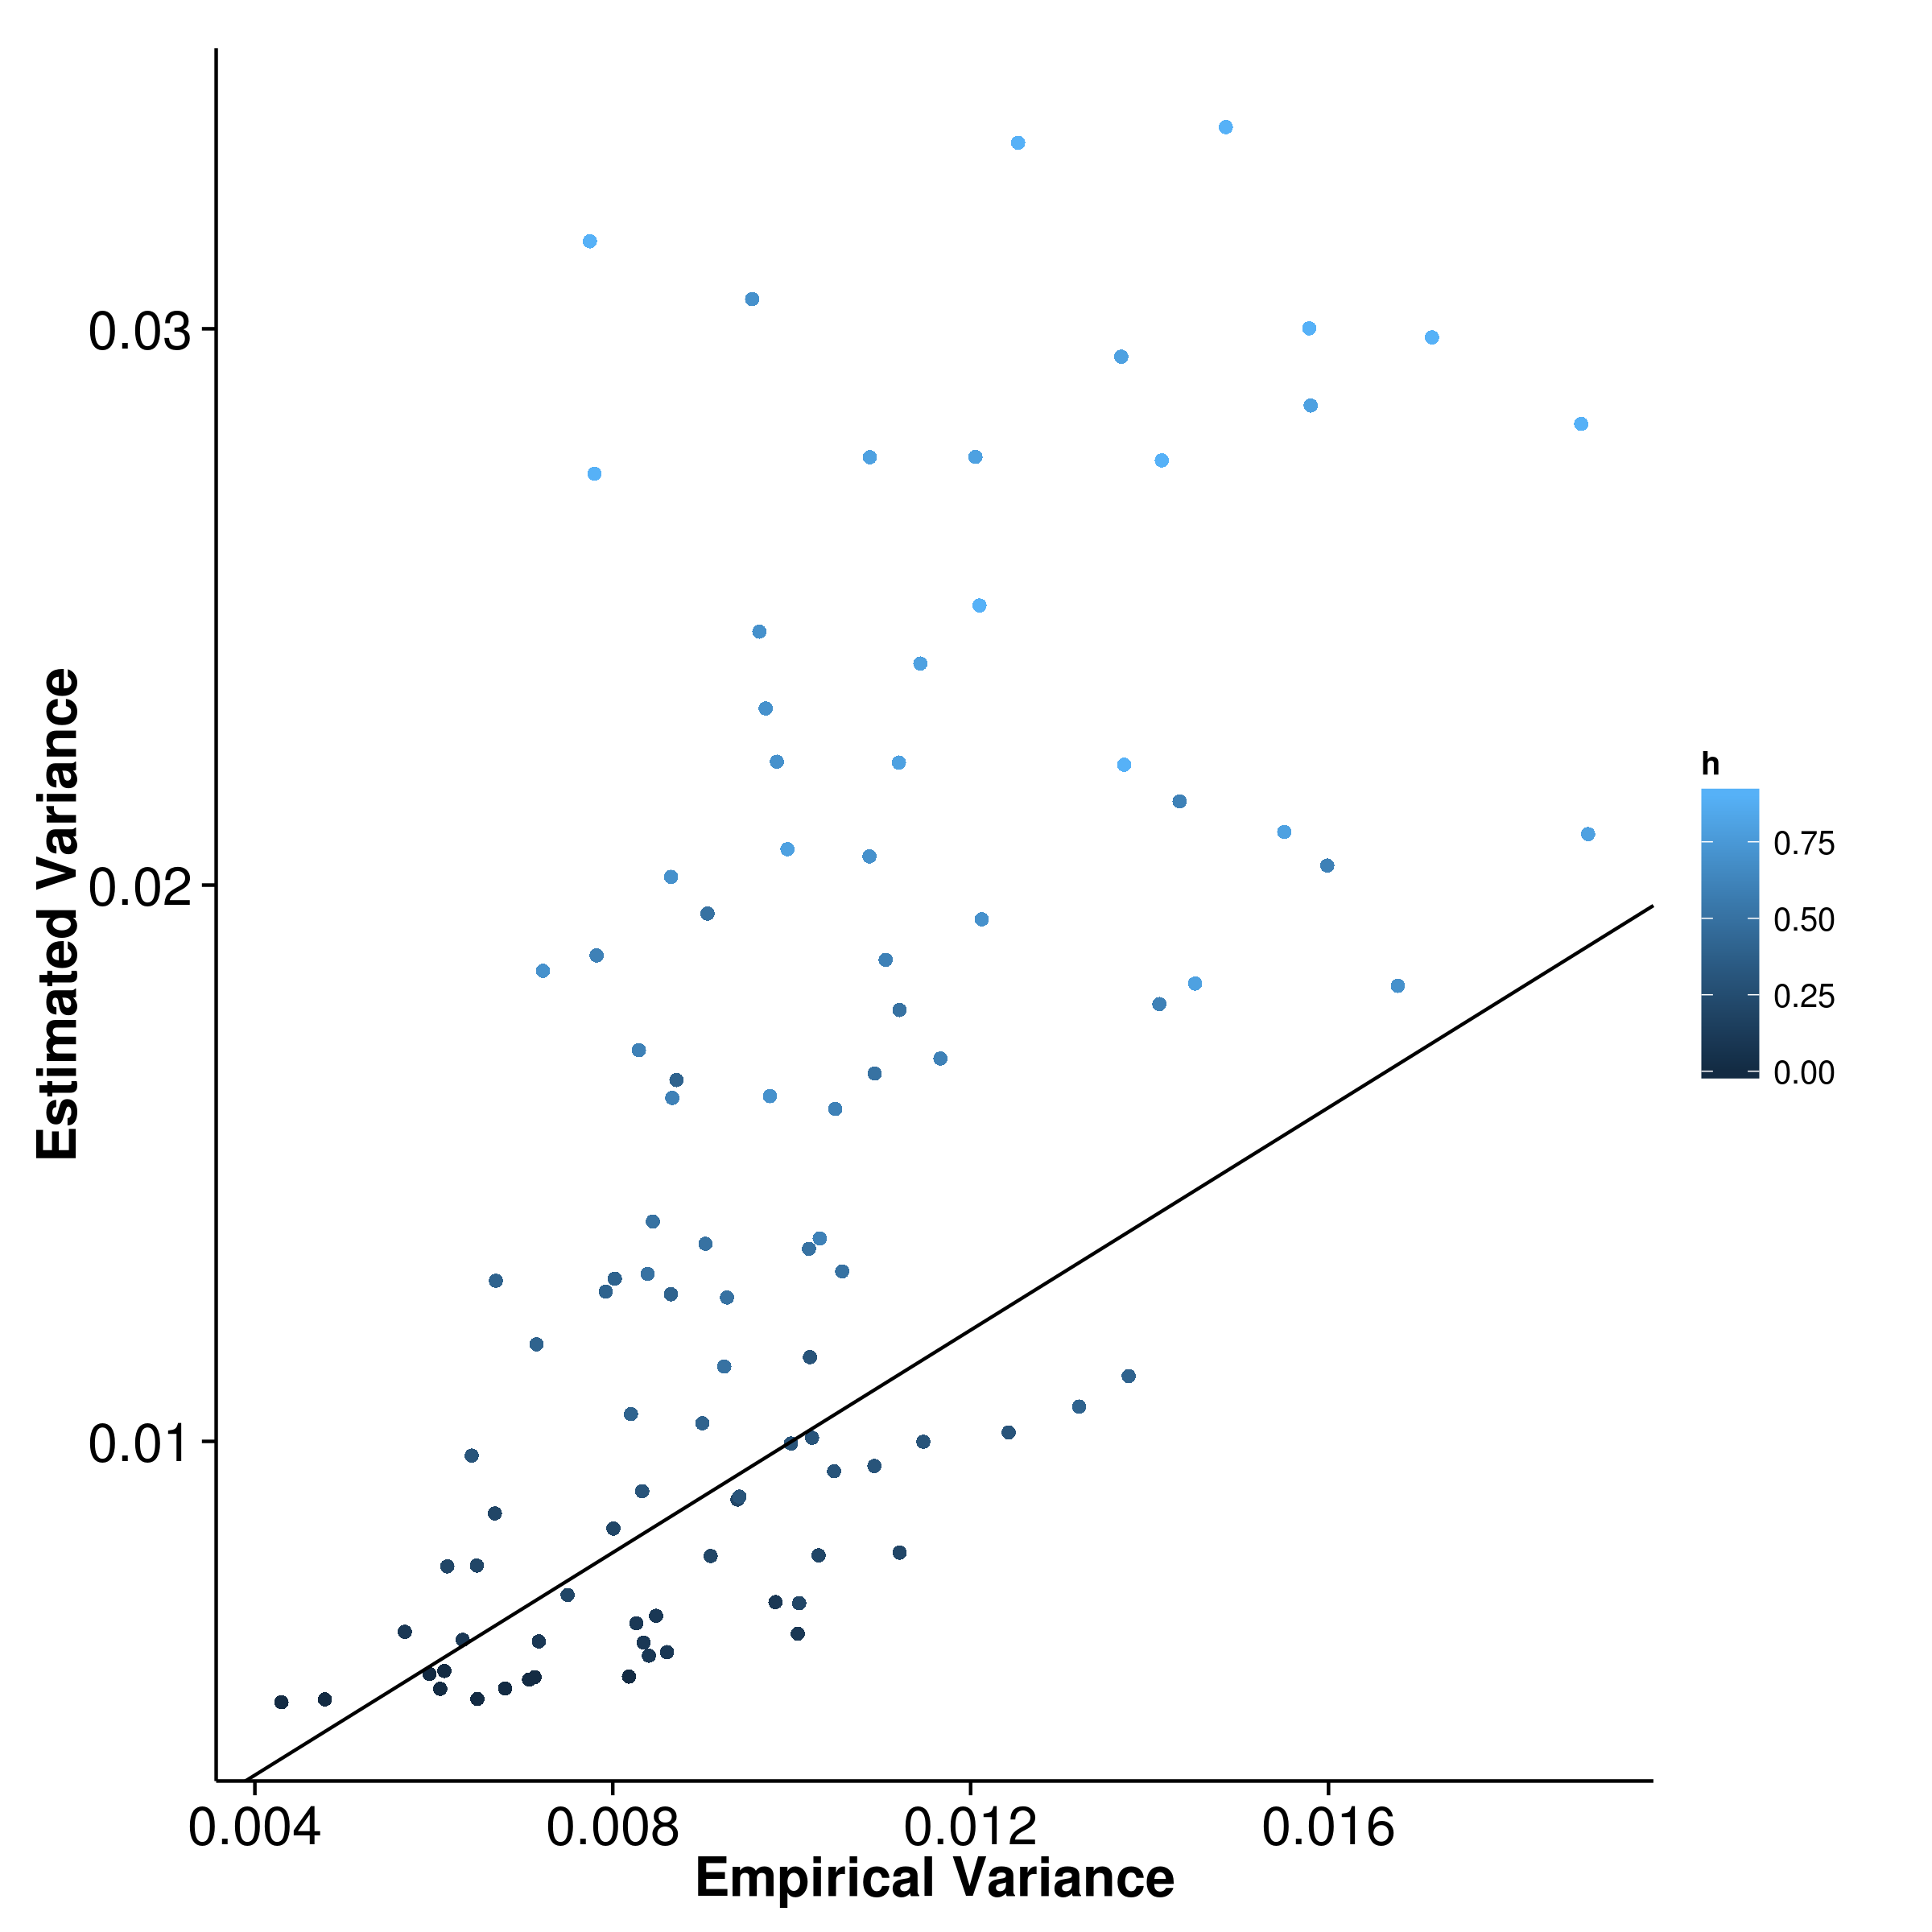
\includegraphics{figure/quantitative/same_effect/100c/ldsc_50k_100c_varH.png}}
			\label{fig:50k100cQtvarL}
		}
		\subfloat[LDSC with intercept estimation]{
			\scalebox{.4}{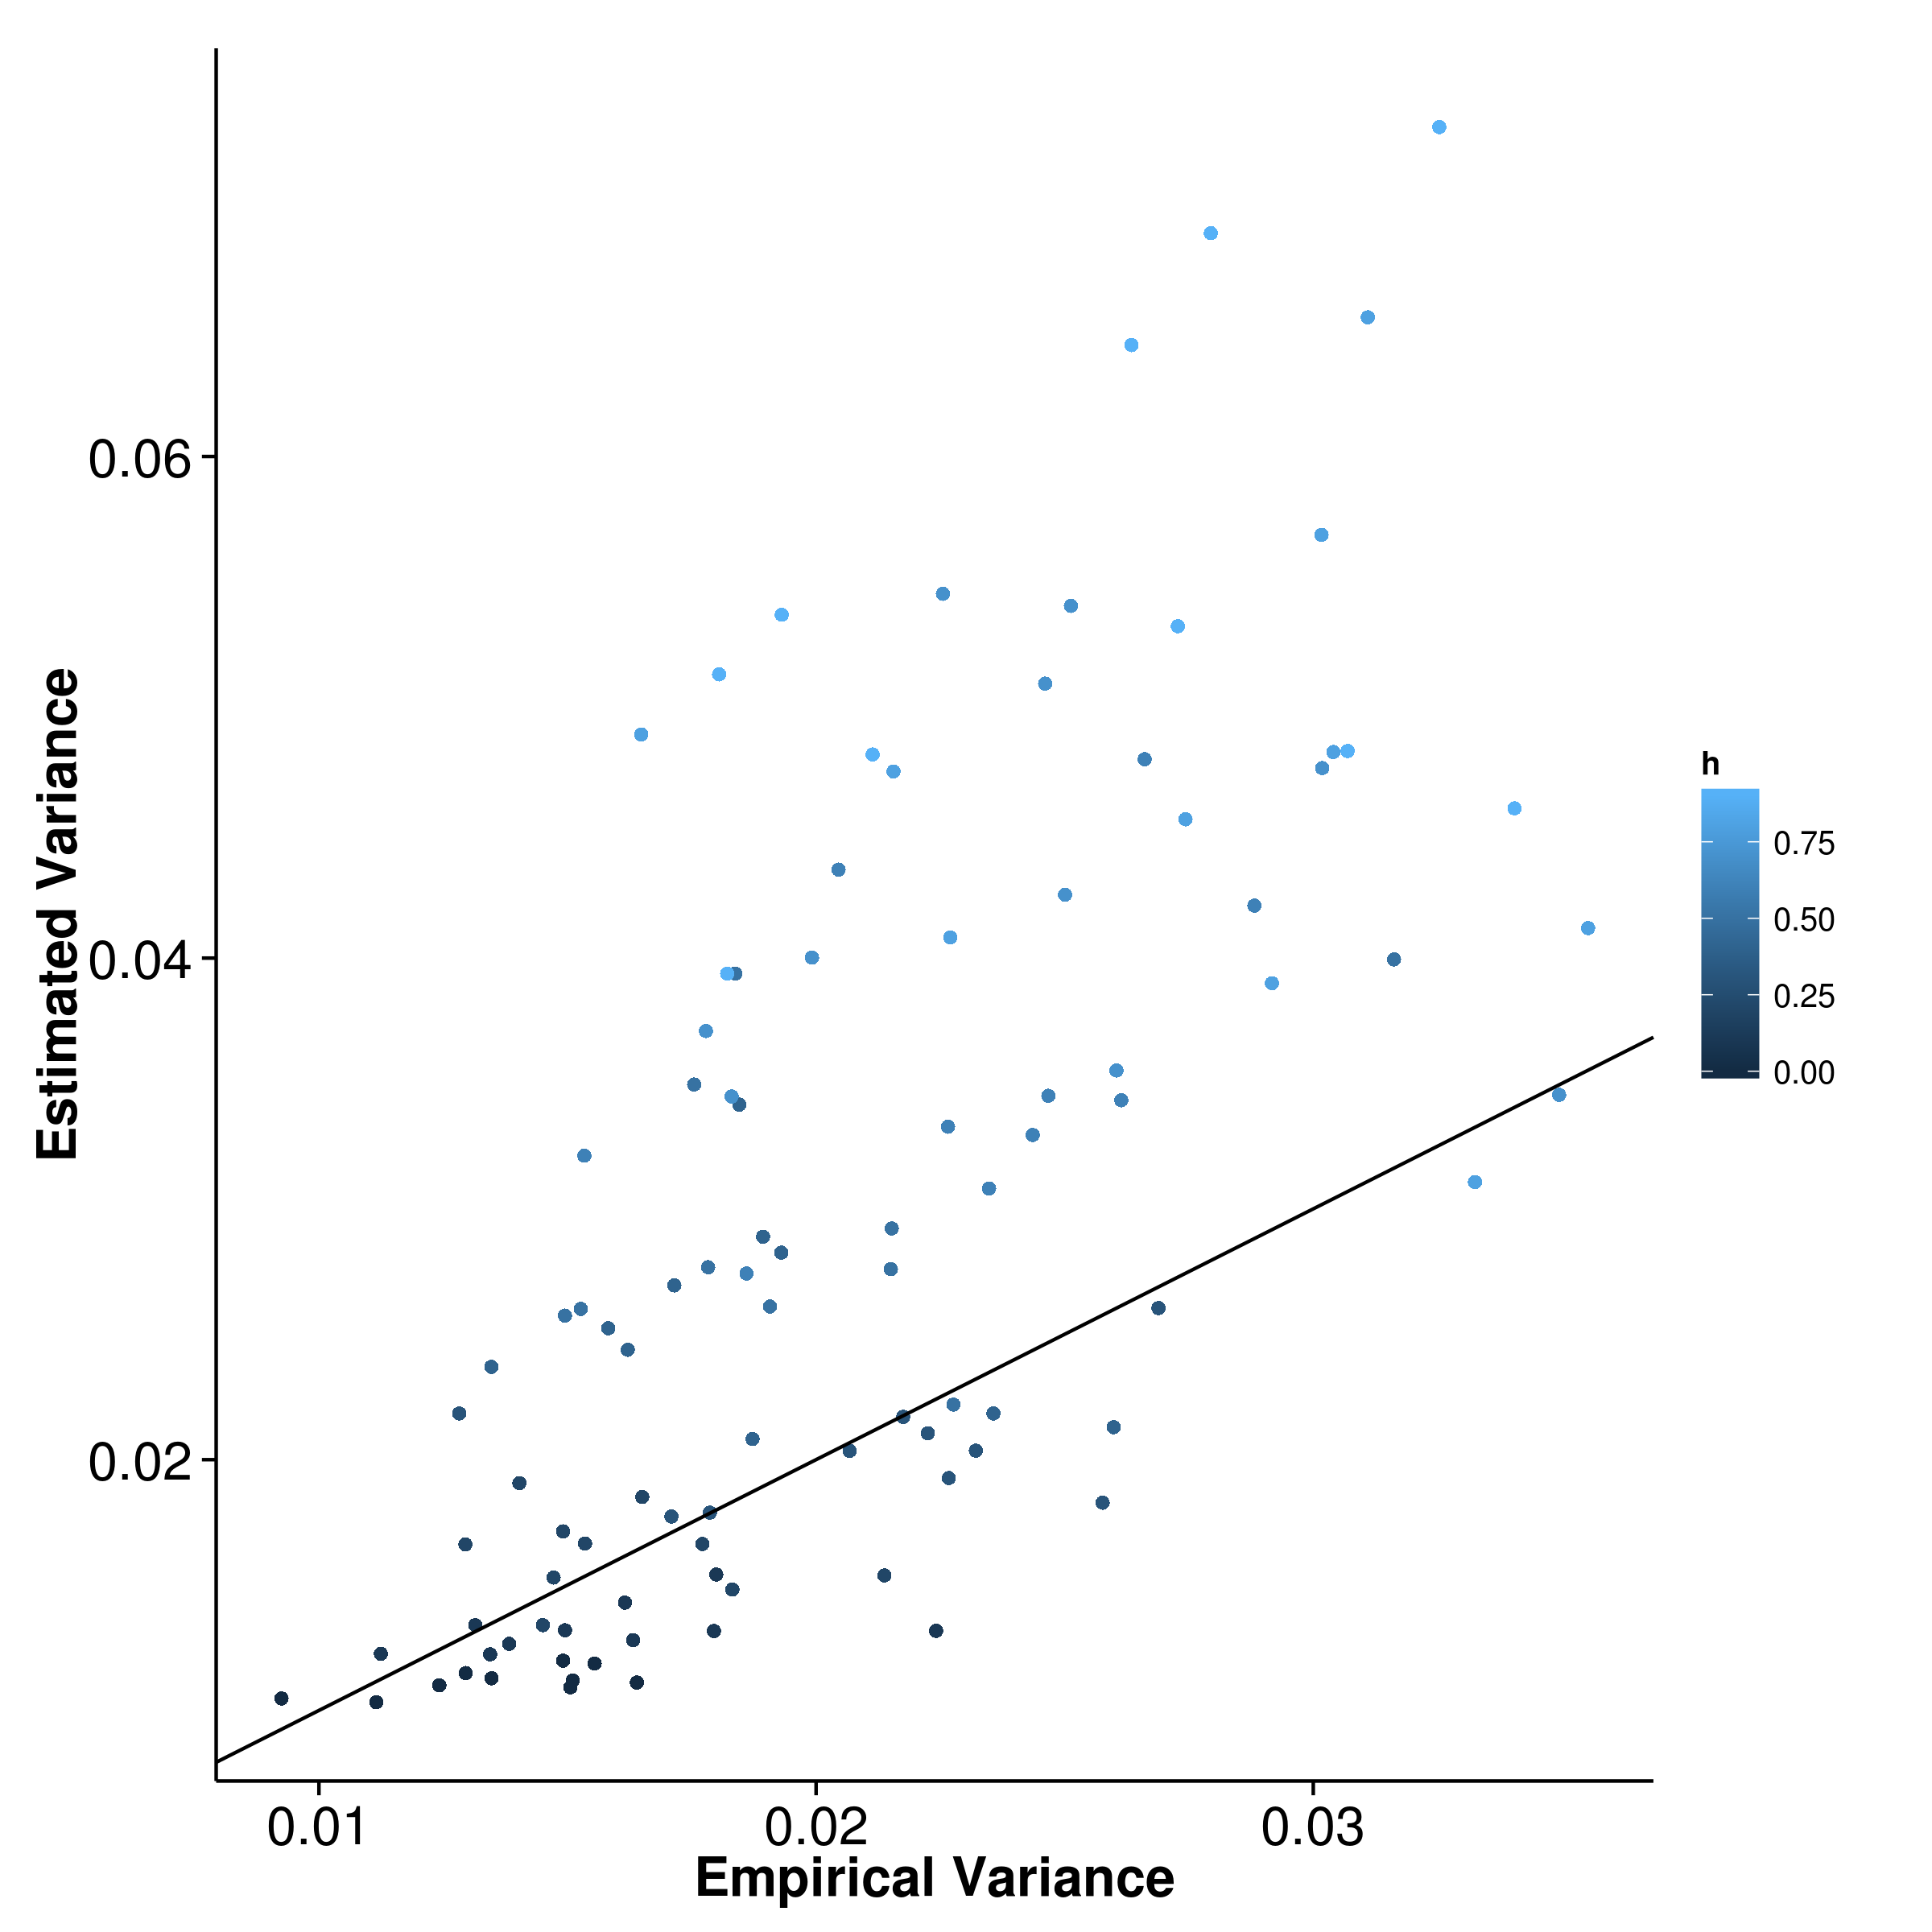
\includegraphics{figure/quantitative/same_effect/100c/ldscIn_50k_100c_varH.png}}
			\label{fig:50k100cQtvarI}
		}
		\label{fig:50k100cQtVar}
	\end{figure}
	
	
	\begin{figure}
		\centering
		\subfloat[SHREK]{
			\scalebox{.4}{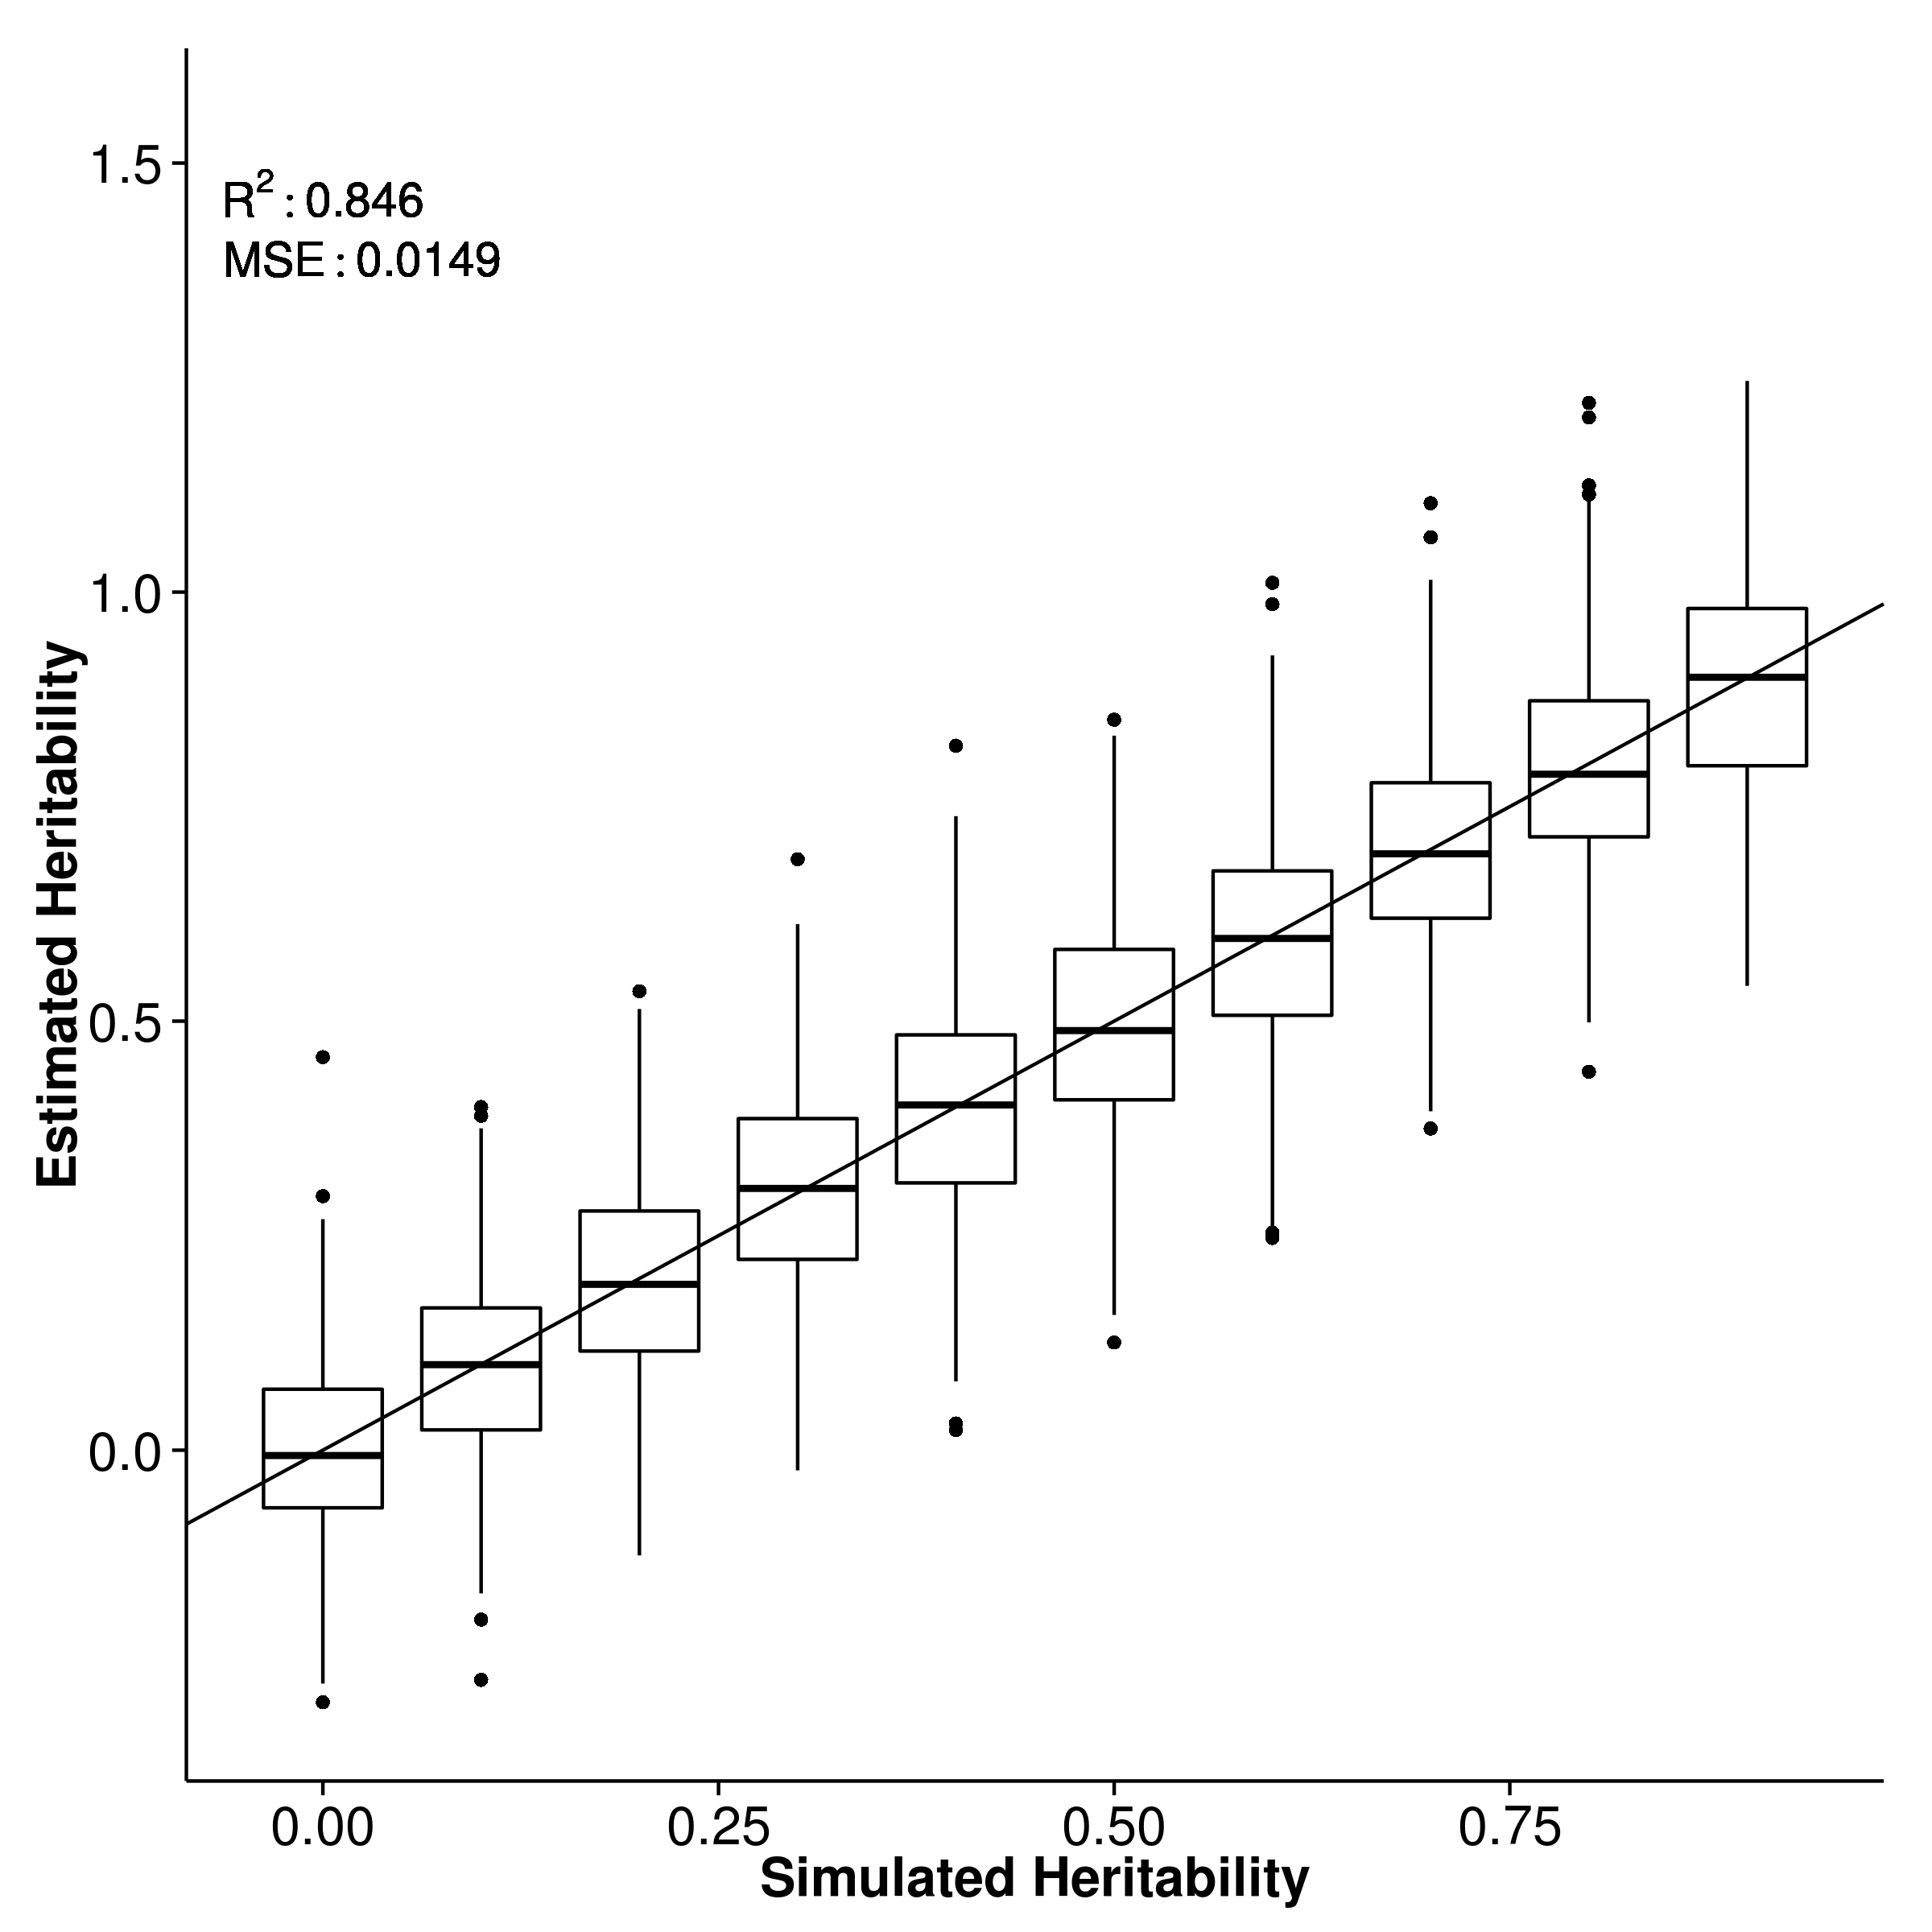
\includegraphics{figure/quantitative/same_effect/250c/shrek_50k_250c_meanH.png}}
			\label{fig:50k250cQtmeanS}
		}
		\subfloat[GCTA]{
			\scalebox{.4}{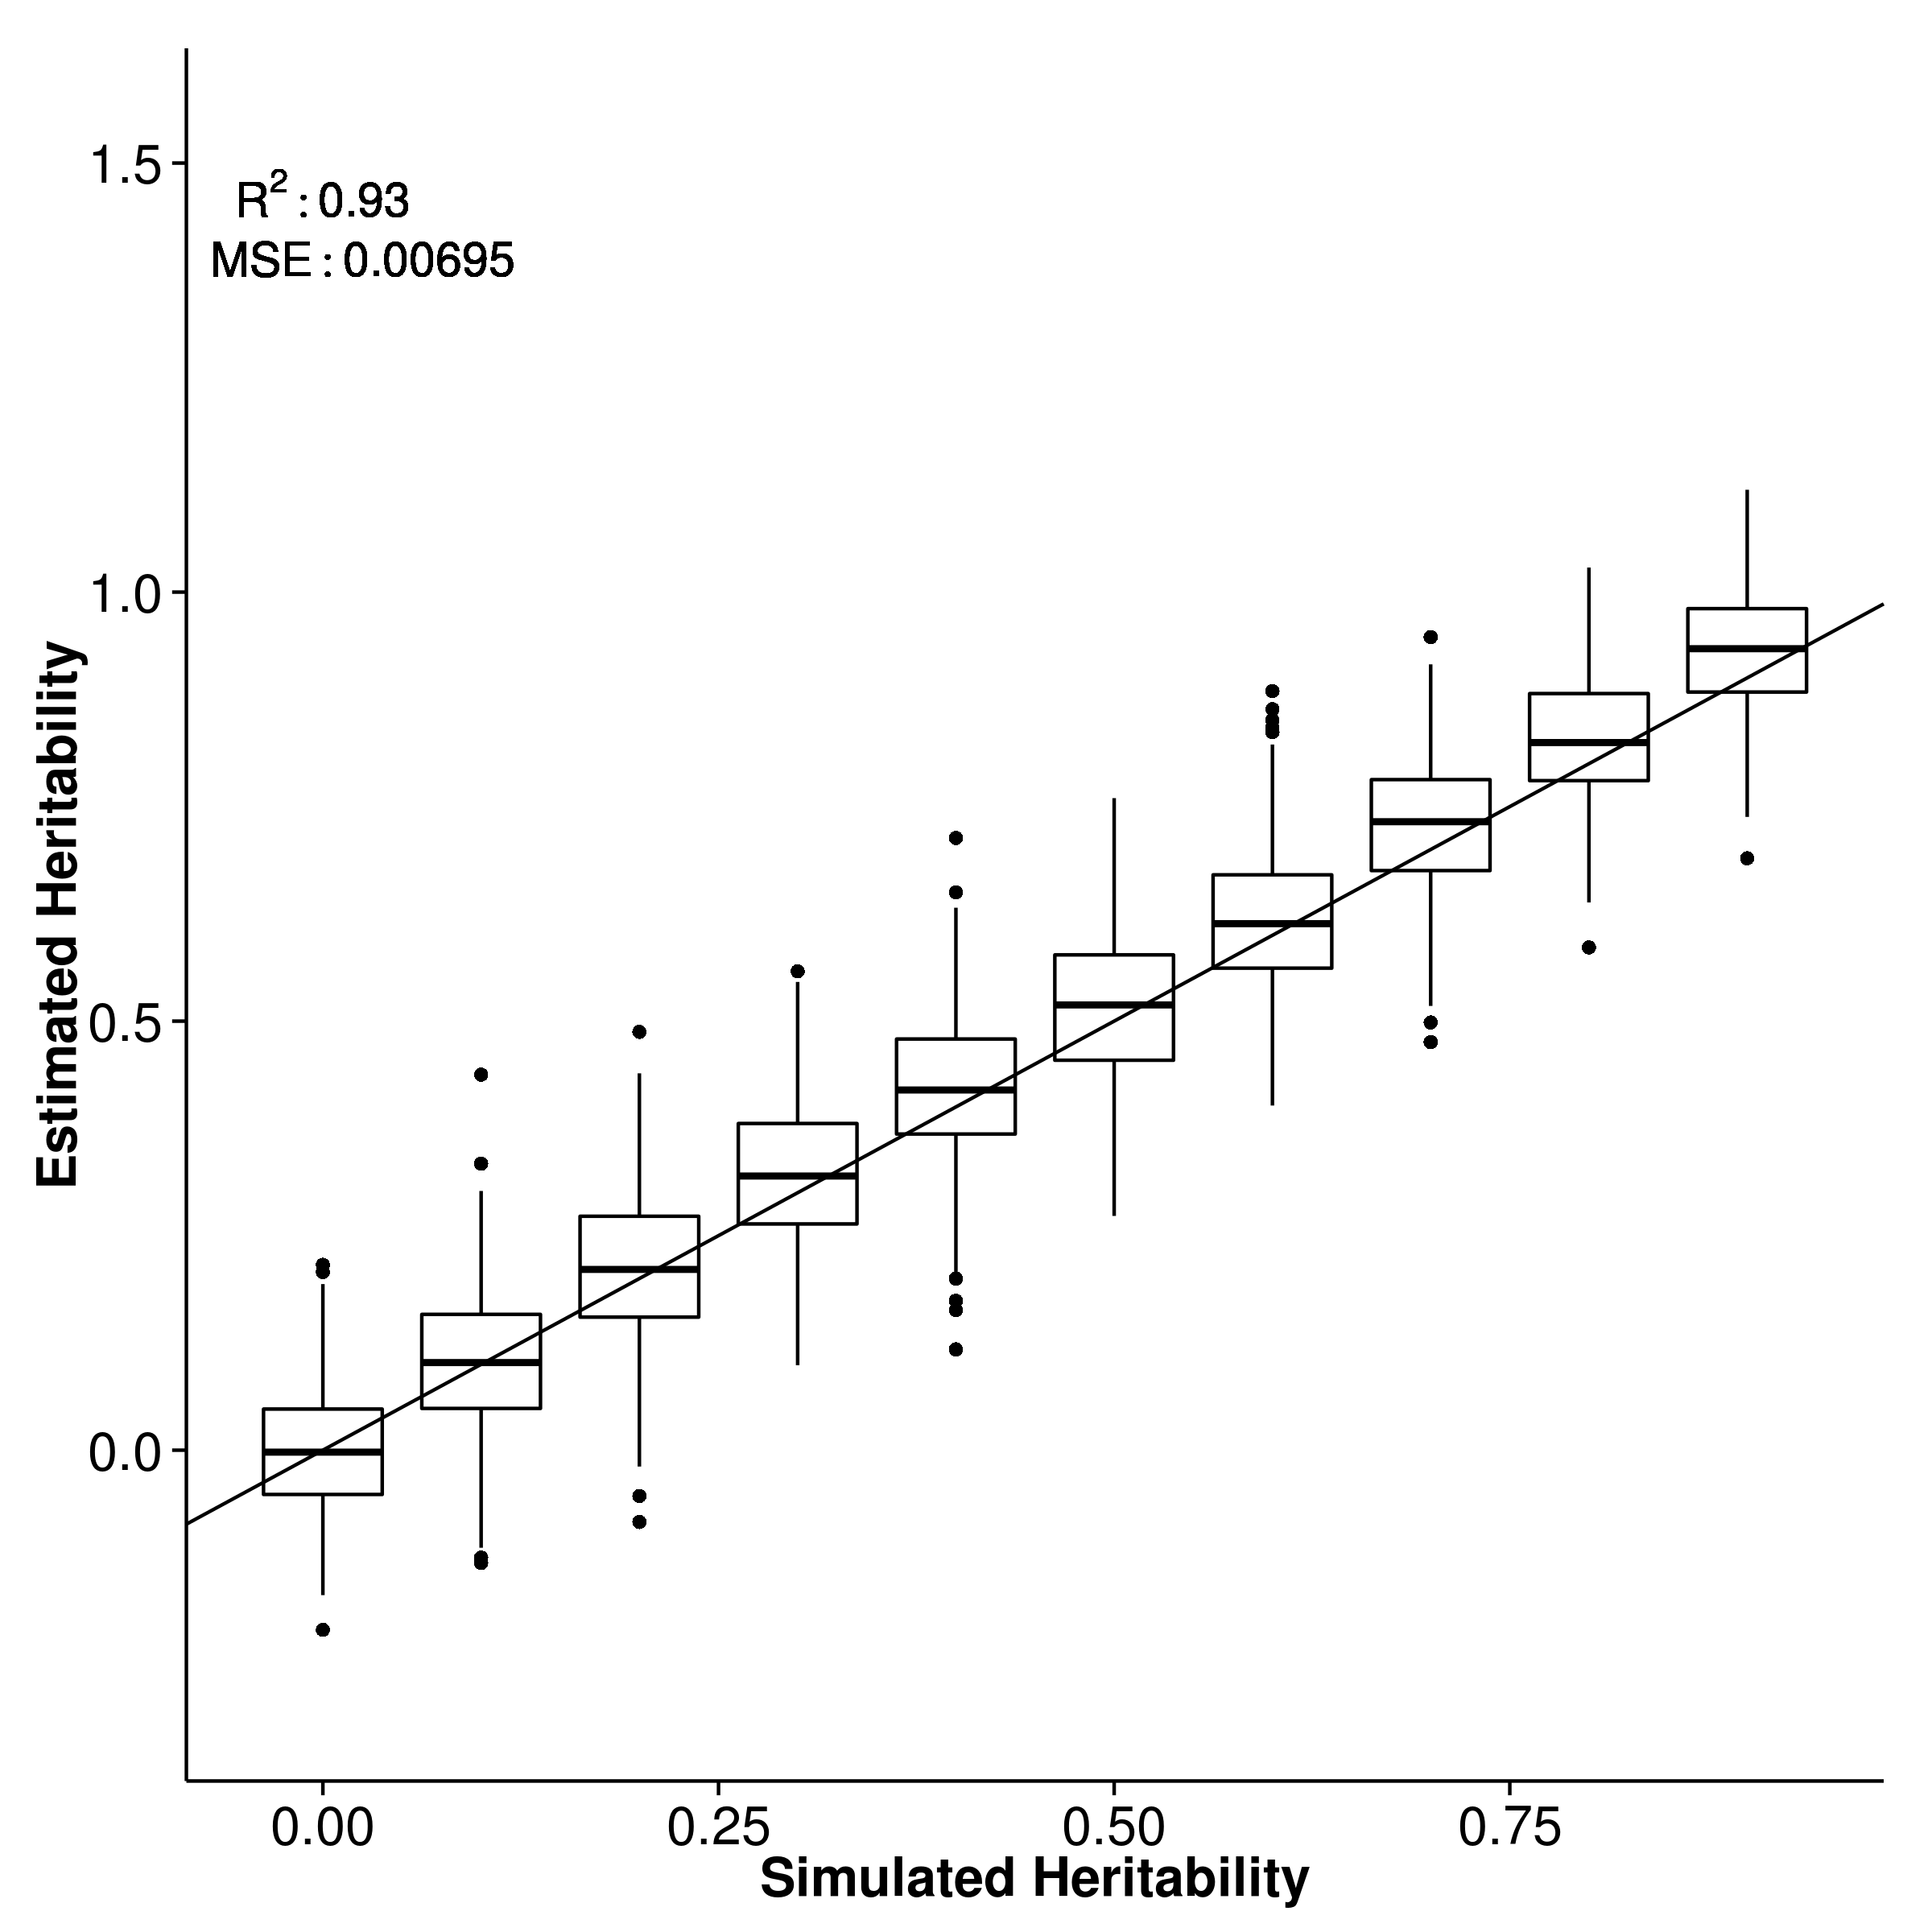
\includegraphics{figure/quantitative/same_effect/250c/gcta_50k_250c_meanH.png}}
			\label{fig:50k250cQtmeanG}
		}\\
		\subfloat[LDSC with fix intercept]{
			\scalebox{.4}{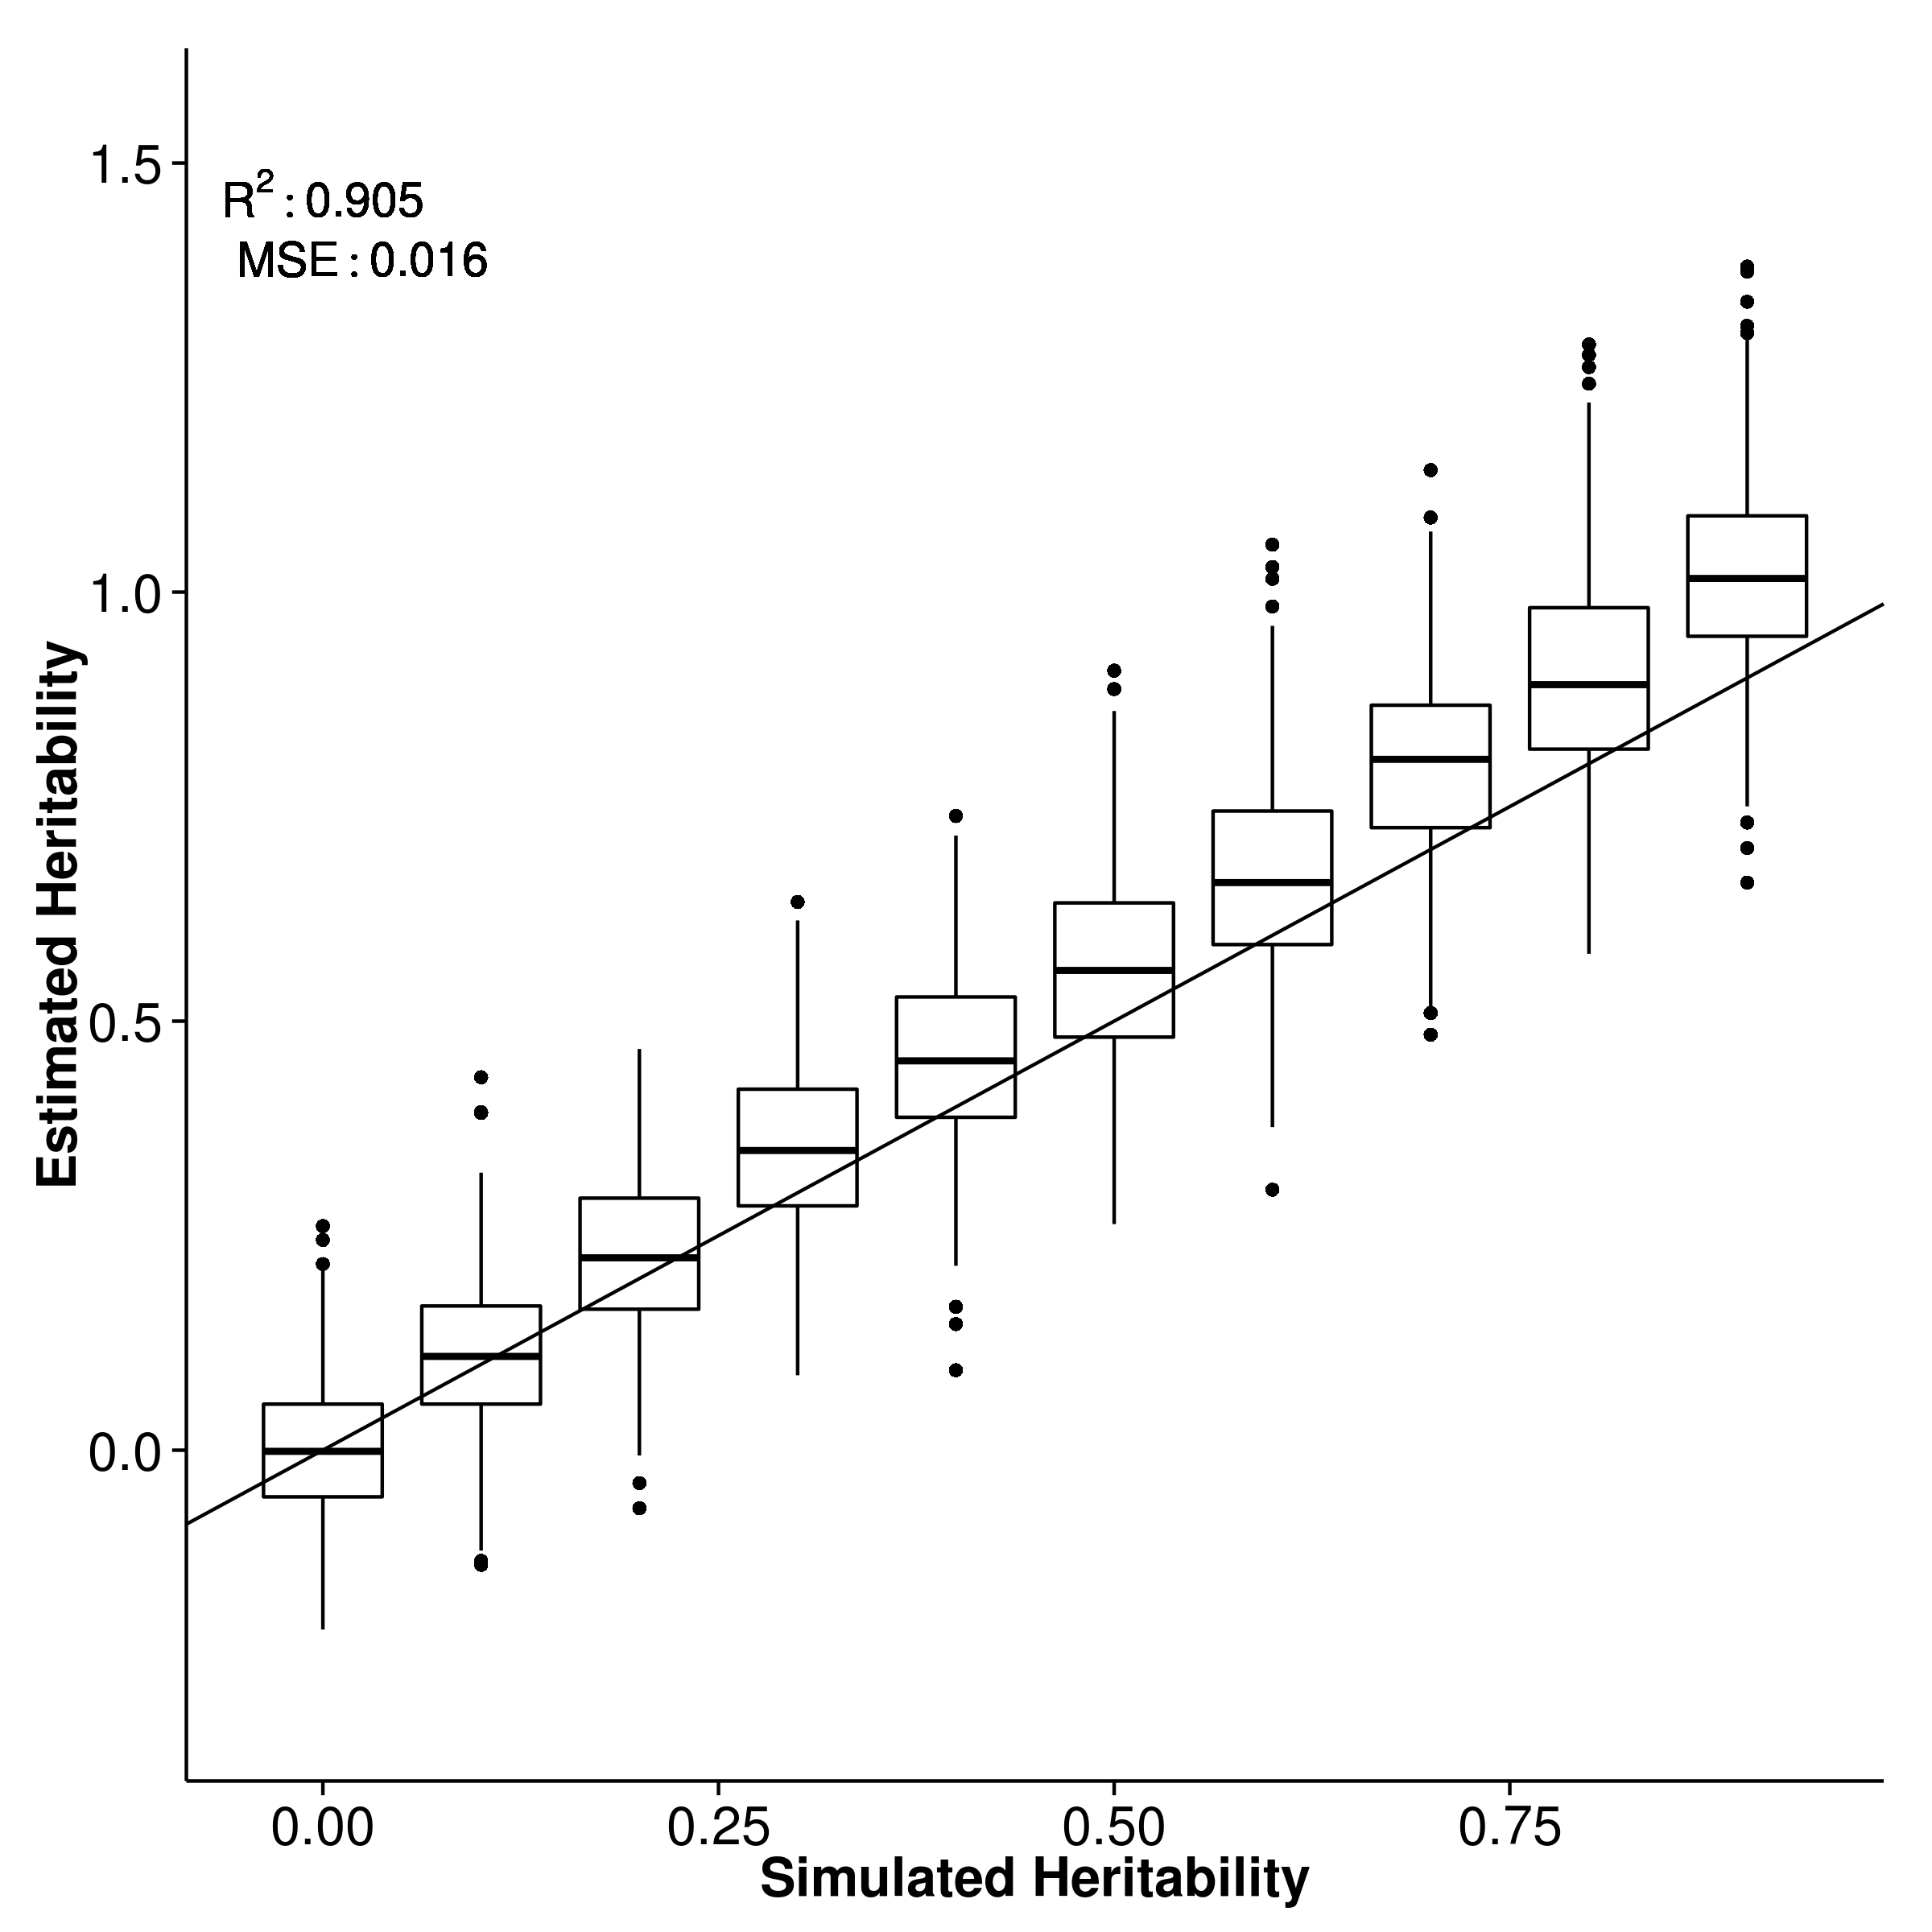
\includegraphics{figure/quantitative/same_effect/250c/ldsc_50k_250c_meanH.png}}
			\label{fig:50k250cQtmeanL}
		}
		\subfloat[LDSC with intercept estimation]{
			\scalebox{.4}{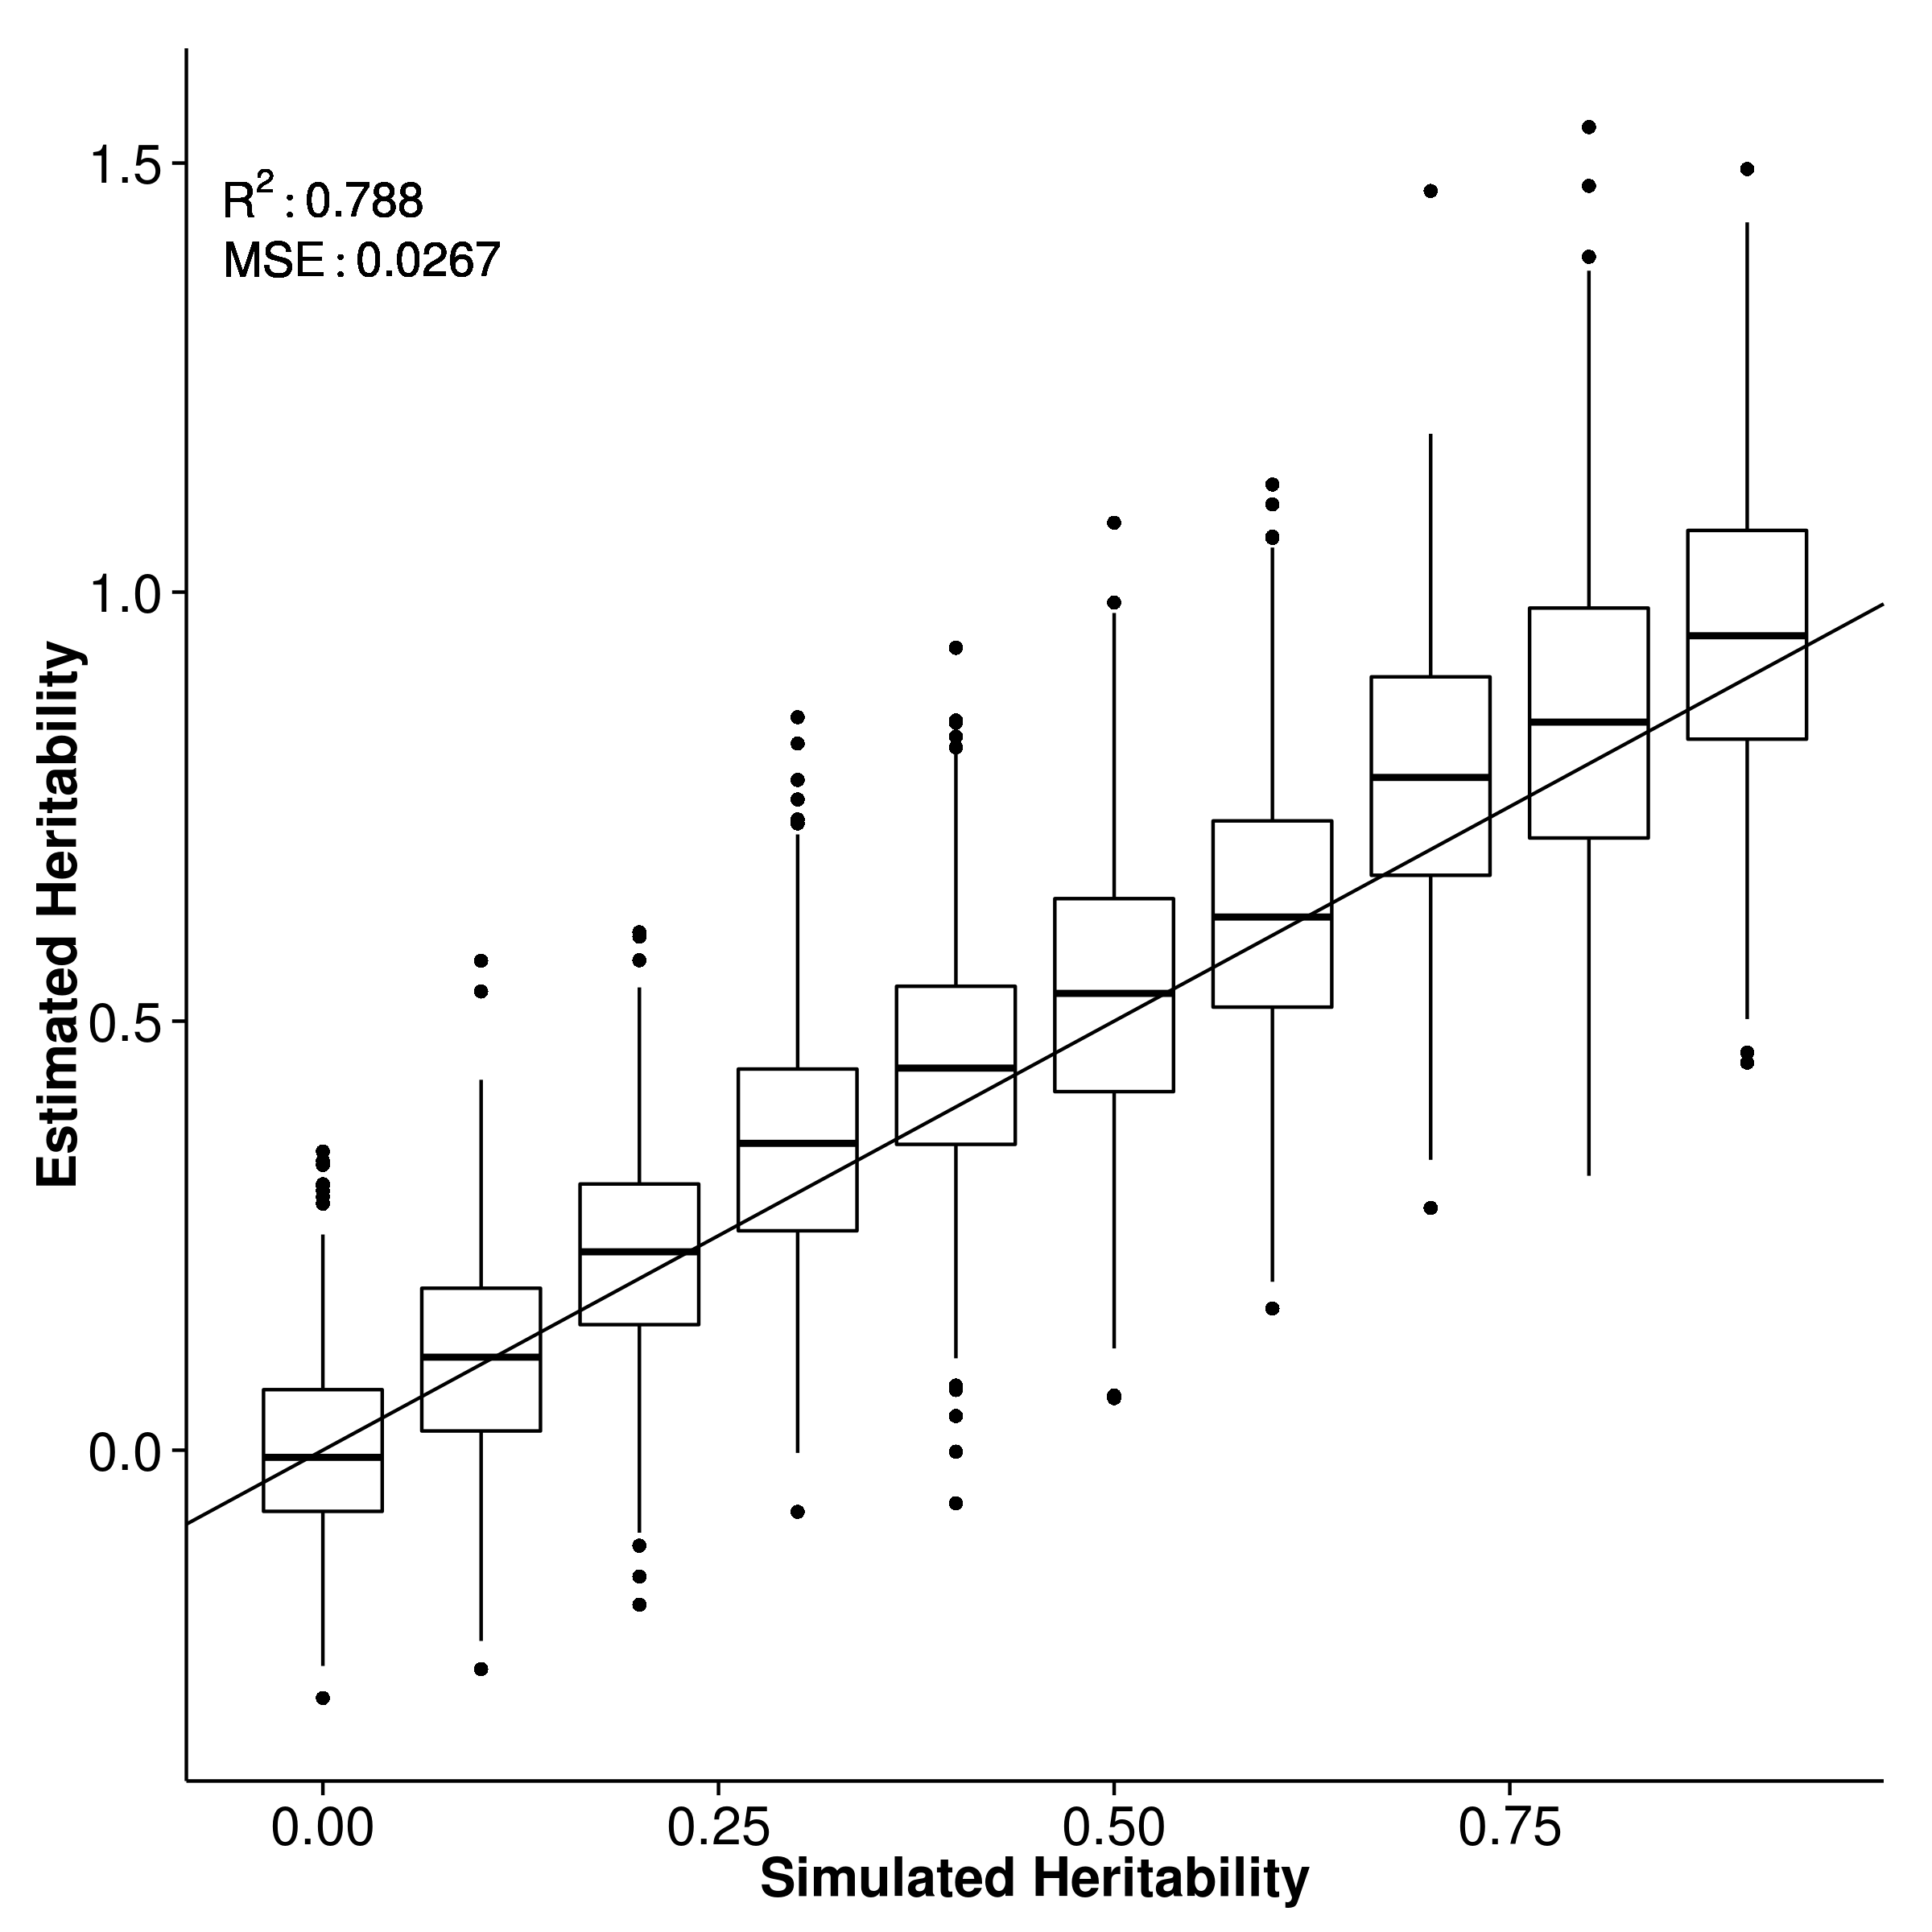
\includegraphics{figure/quantitative/same_effect/250c/ldscIn_50k_250c_meanH.png}}
			\label{fig:50k250cQtmeanI}
		}
		\caption[Simulation of Quantitative Traits with 50k \glsentryshortpl{SNP} and 250 causal variants of same effect size]
		{Simulation of Quantitative Traits with 50k \glsentryshortpl{SNP} and 250 causal variants with same effect size.} 
		\label{fig:50k250cQtMean}
	\end{figure}
	\begin{figure}
		\centering
		\subfloat[SHREK]{
			\scalebox{.4}{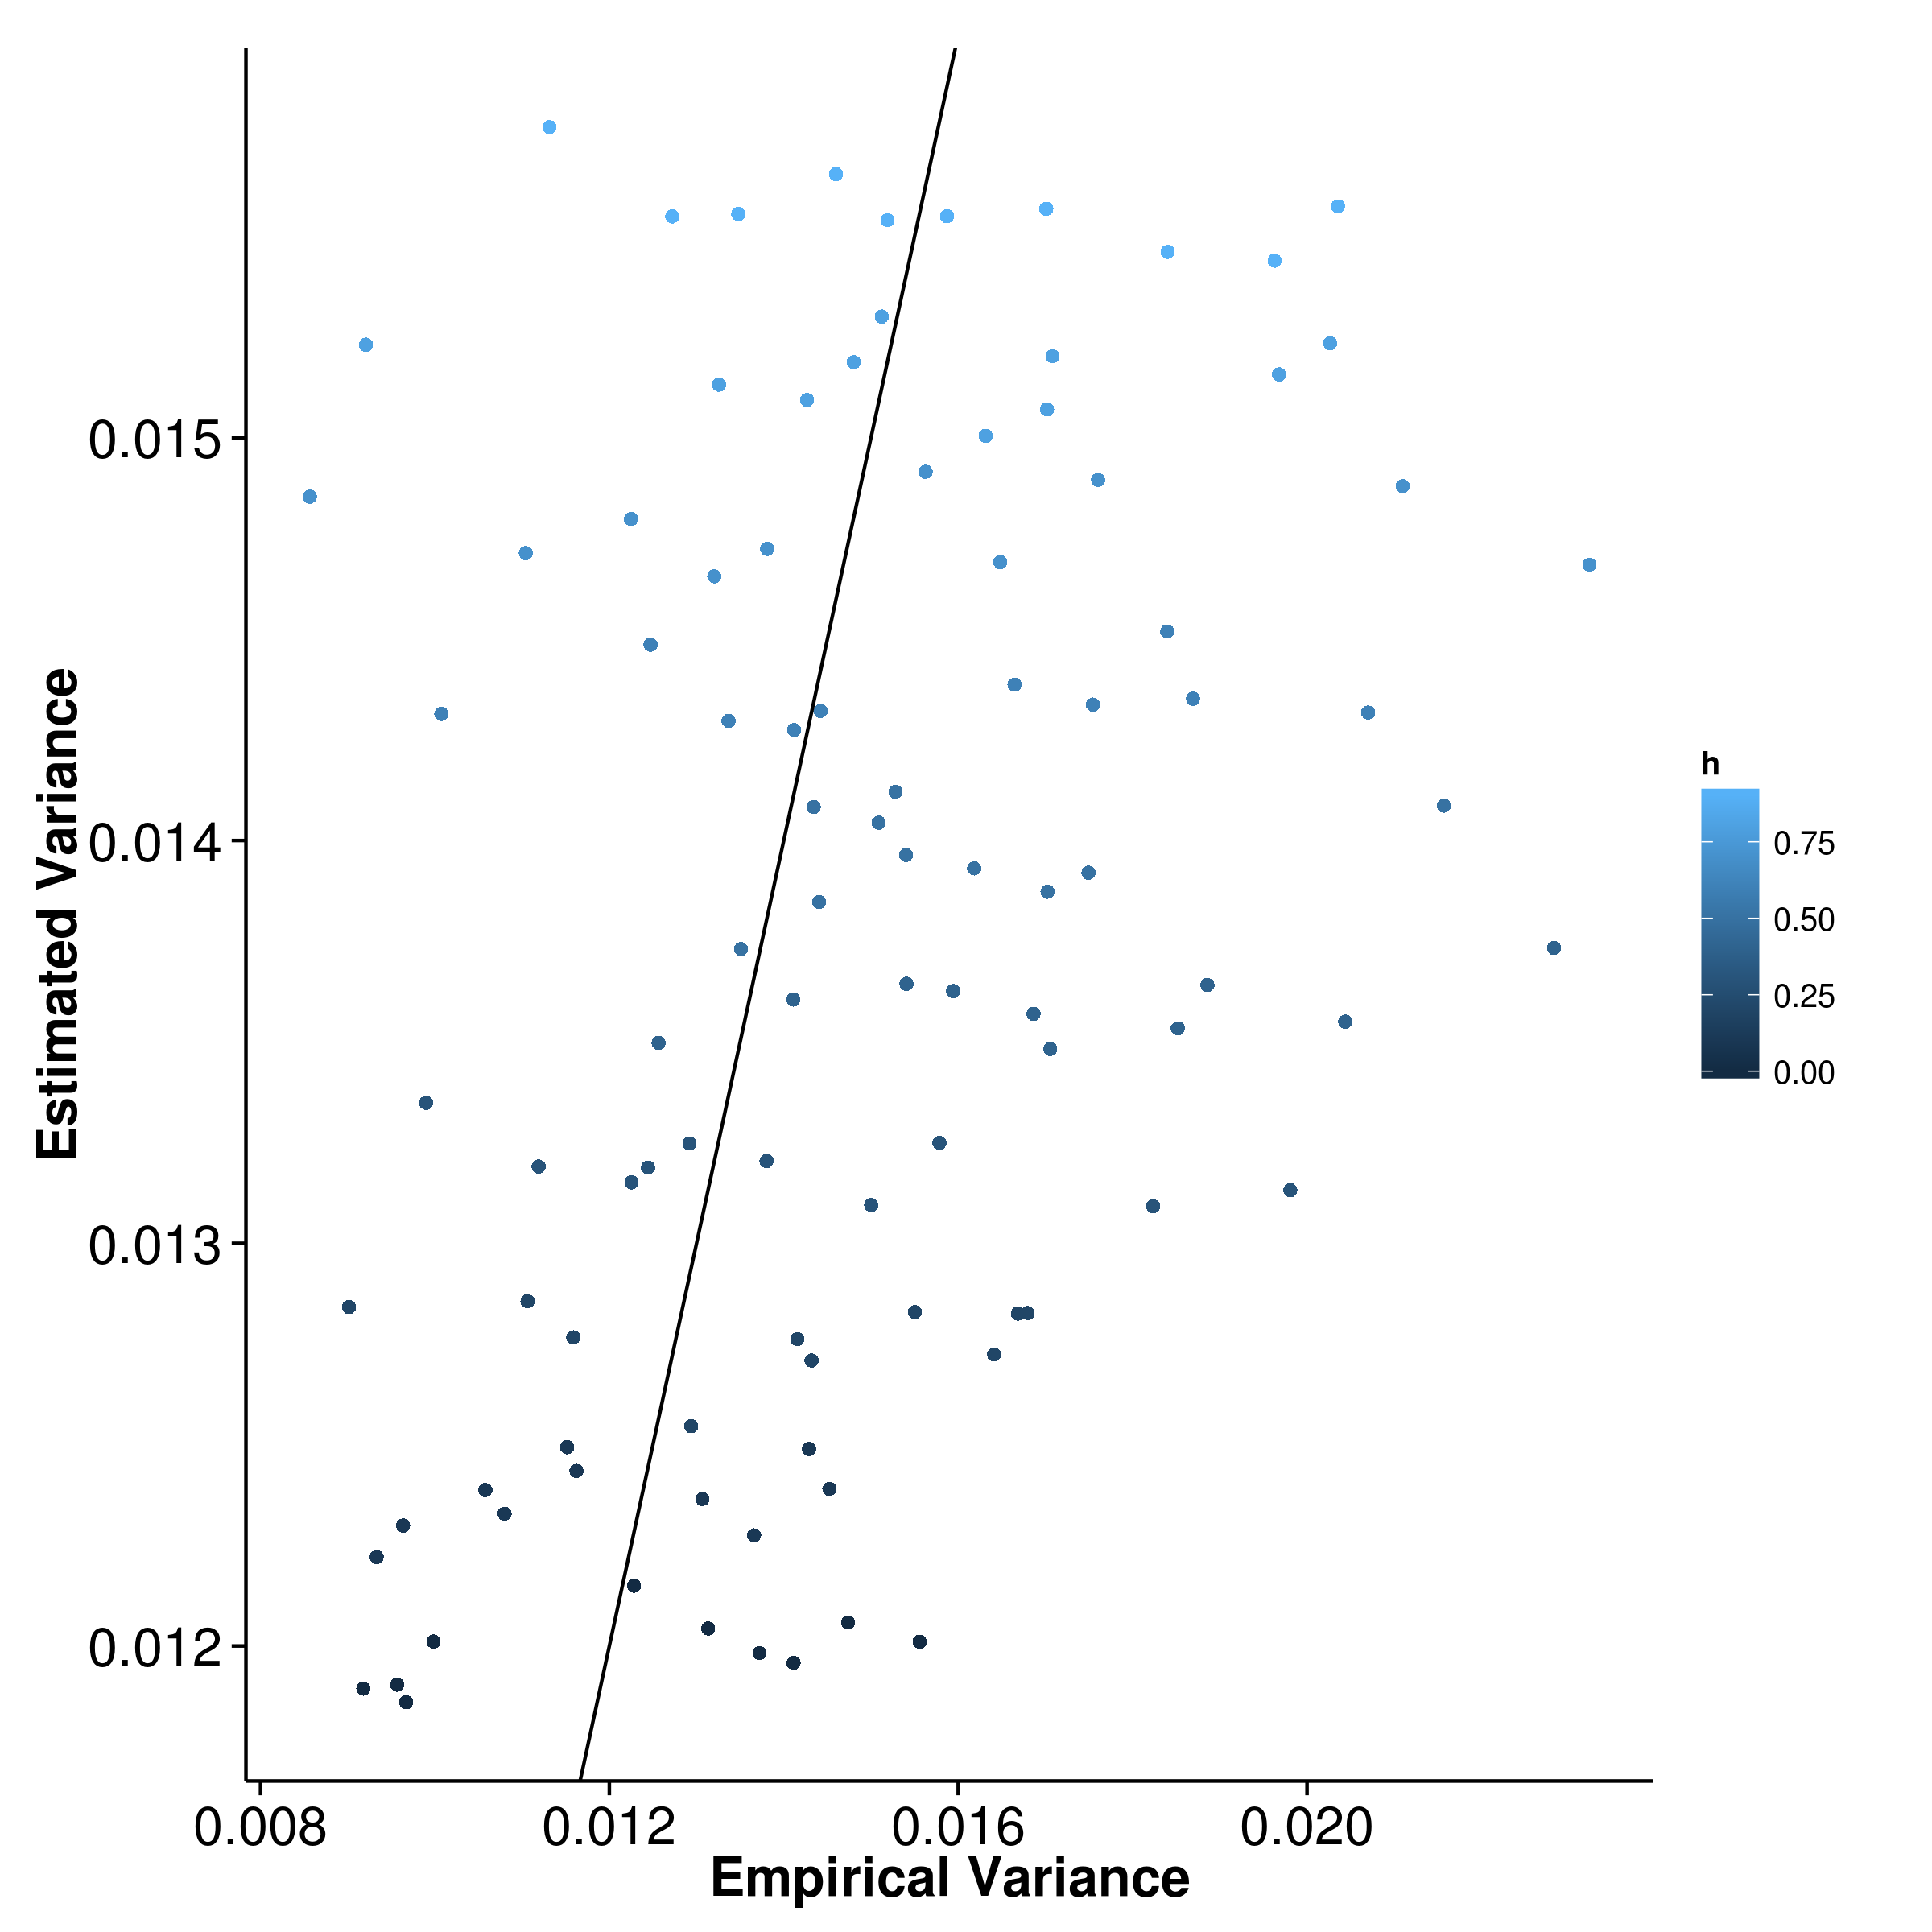
\includegraphics{figure/quantitative/same_effect/250c/shrek_50k_250c_varH.png}}
			\label{fig:50k250cQtvarS}
		}
		\subfloat[GCTA]{
			\scalebox{.4}{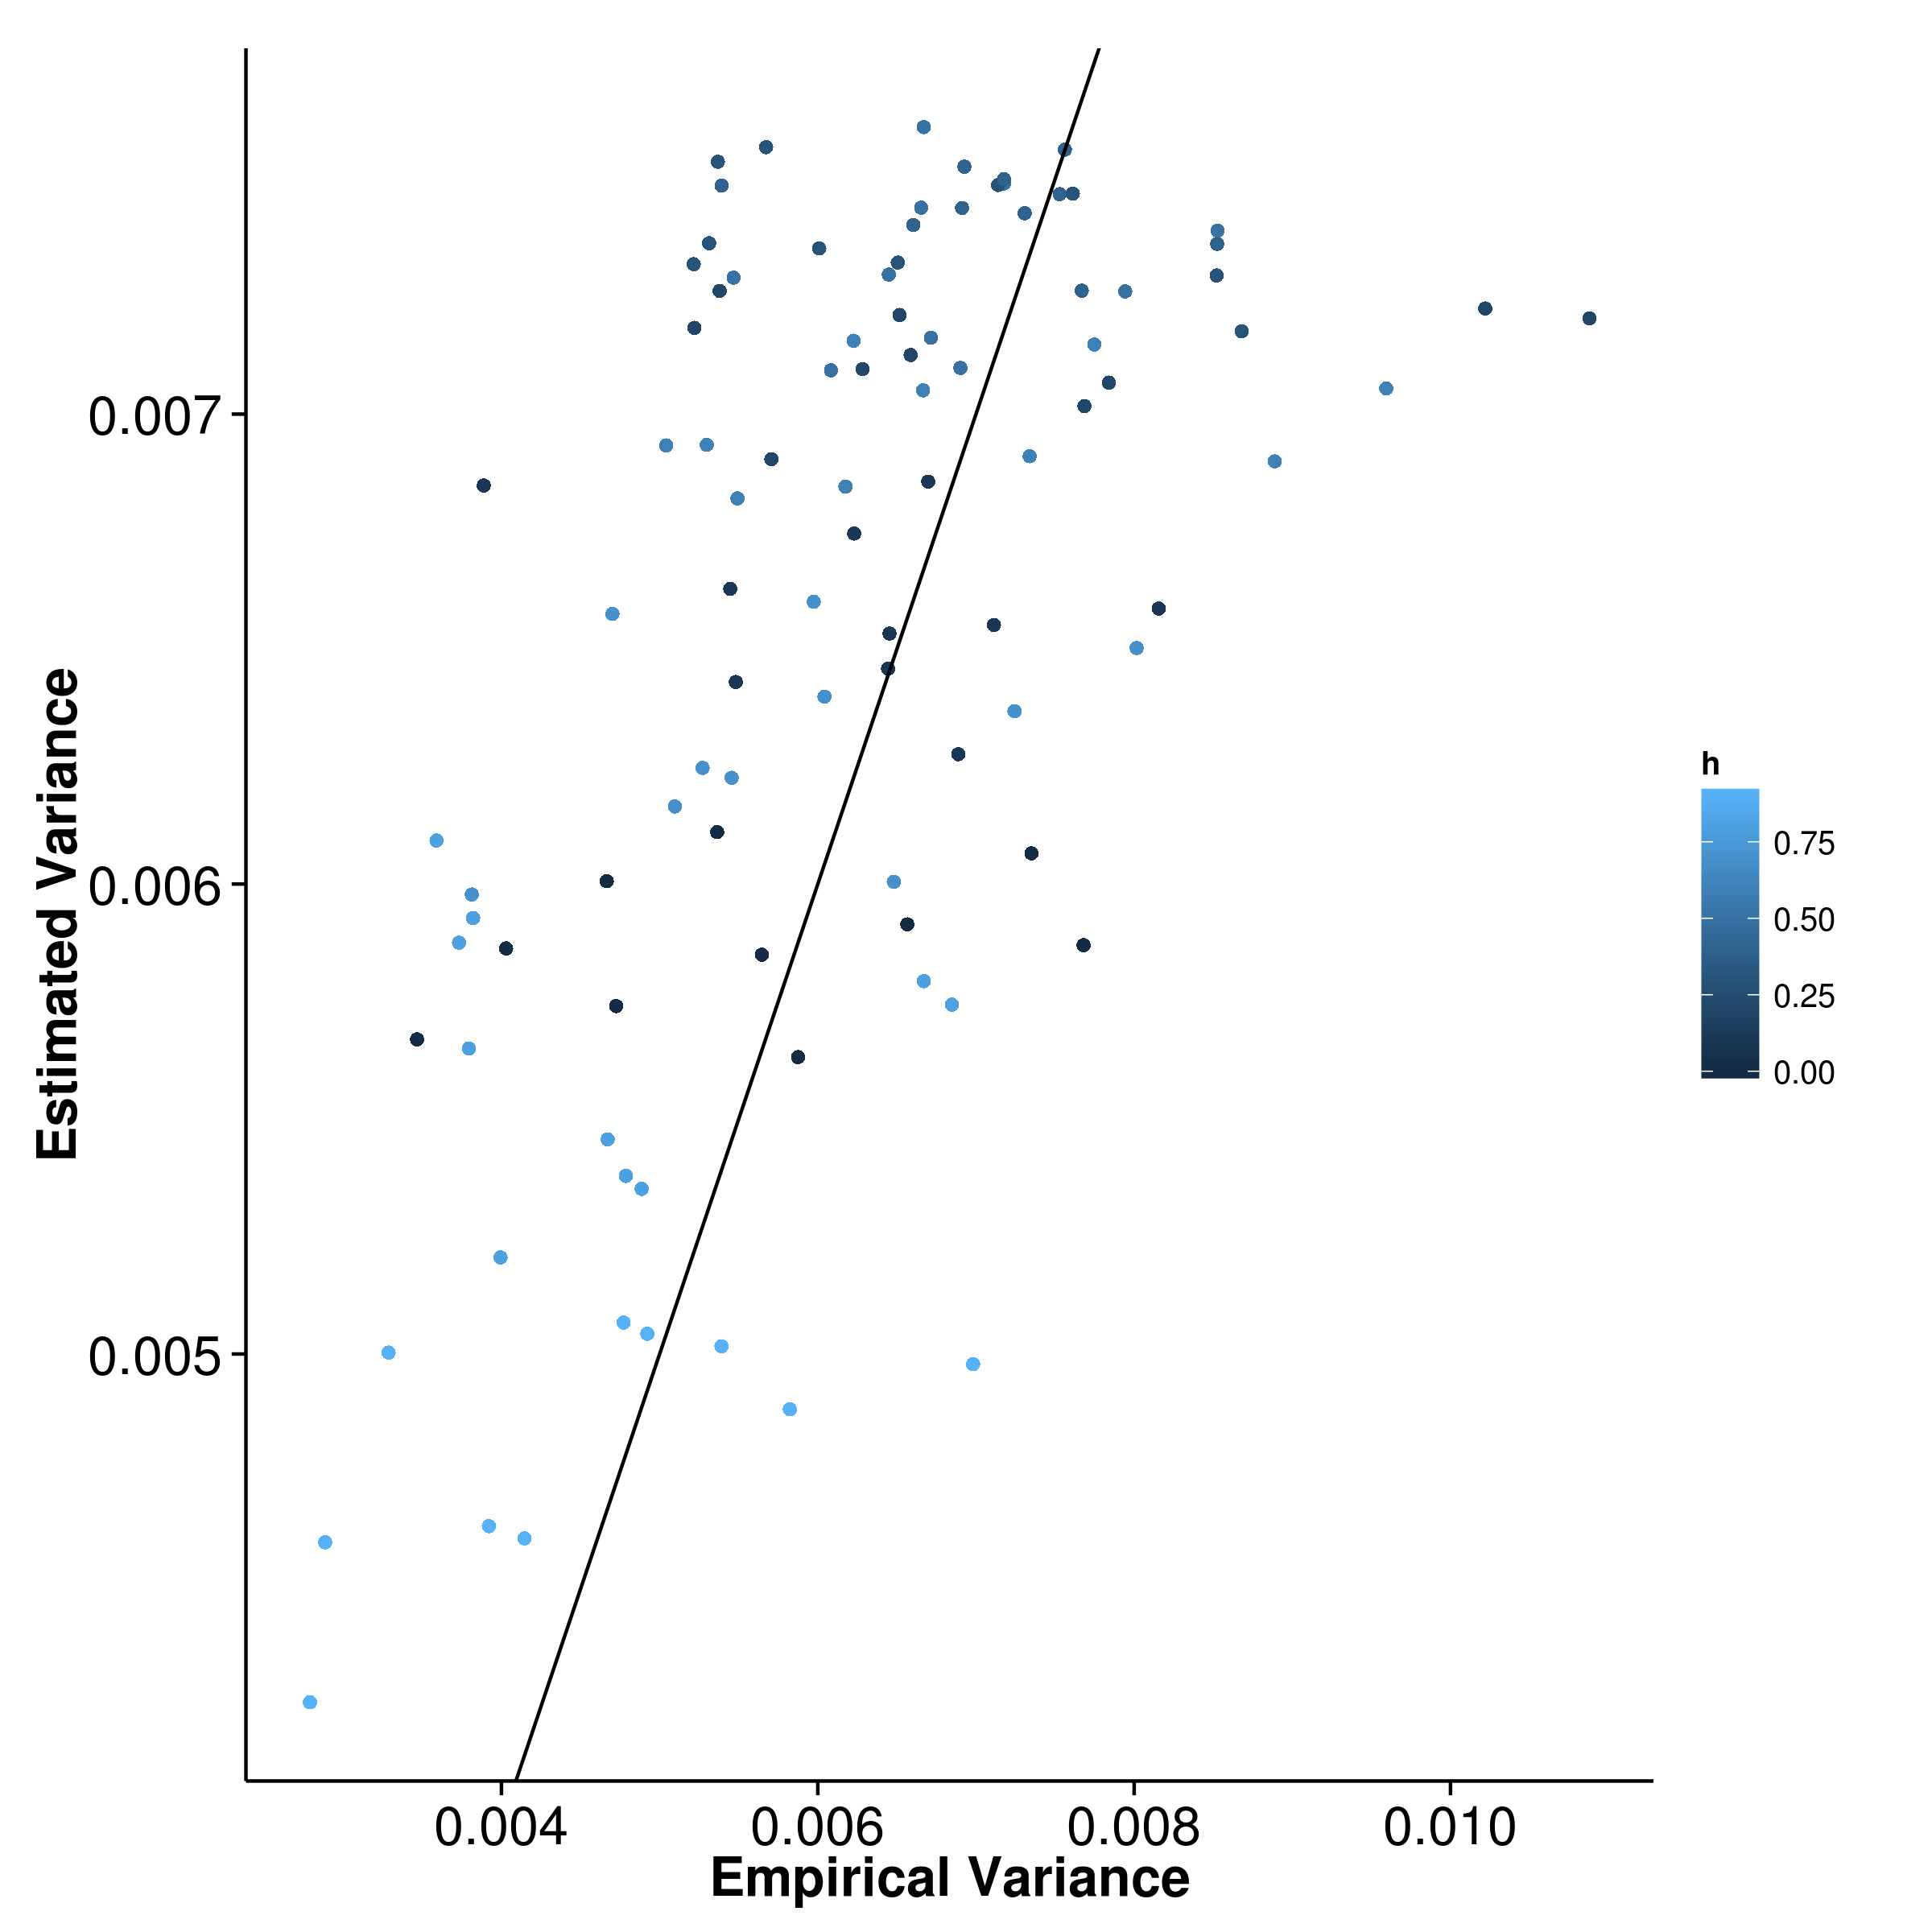
\includegraphics{figure/quantitative/same_effect/250c/gcta_50k_250c_varH.png}}
			\label{fig:50k250cQtvarG}
		}\\
		\subfloat[LDSC with fix intercept]{
			\scalebox{.4}{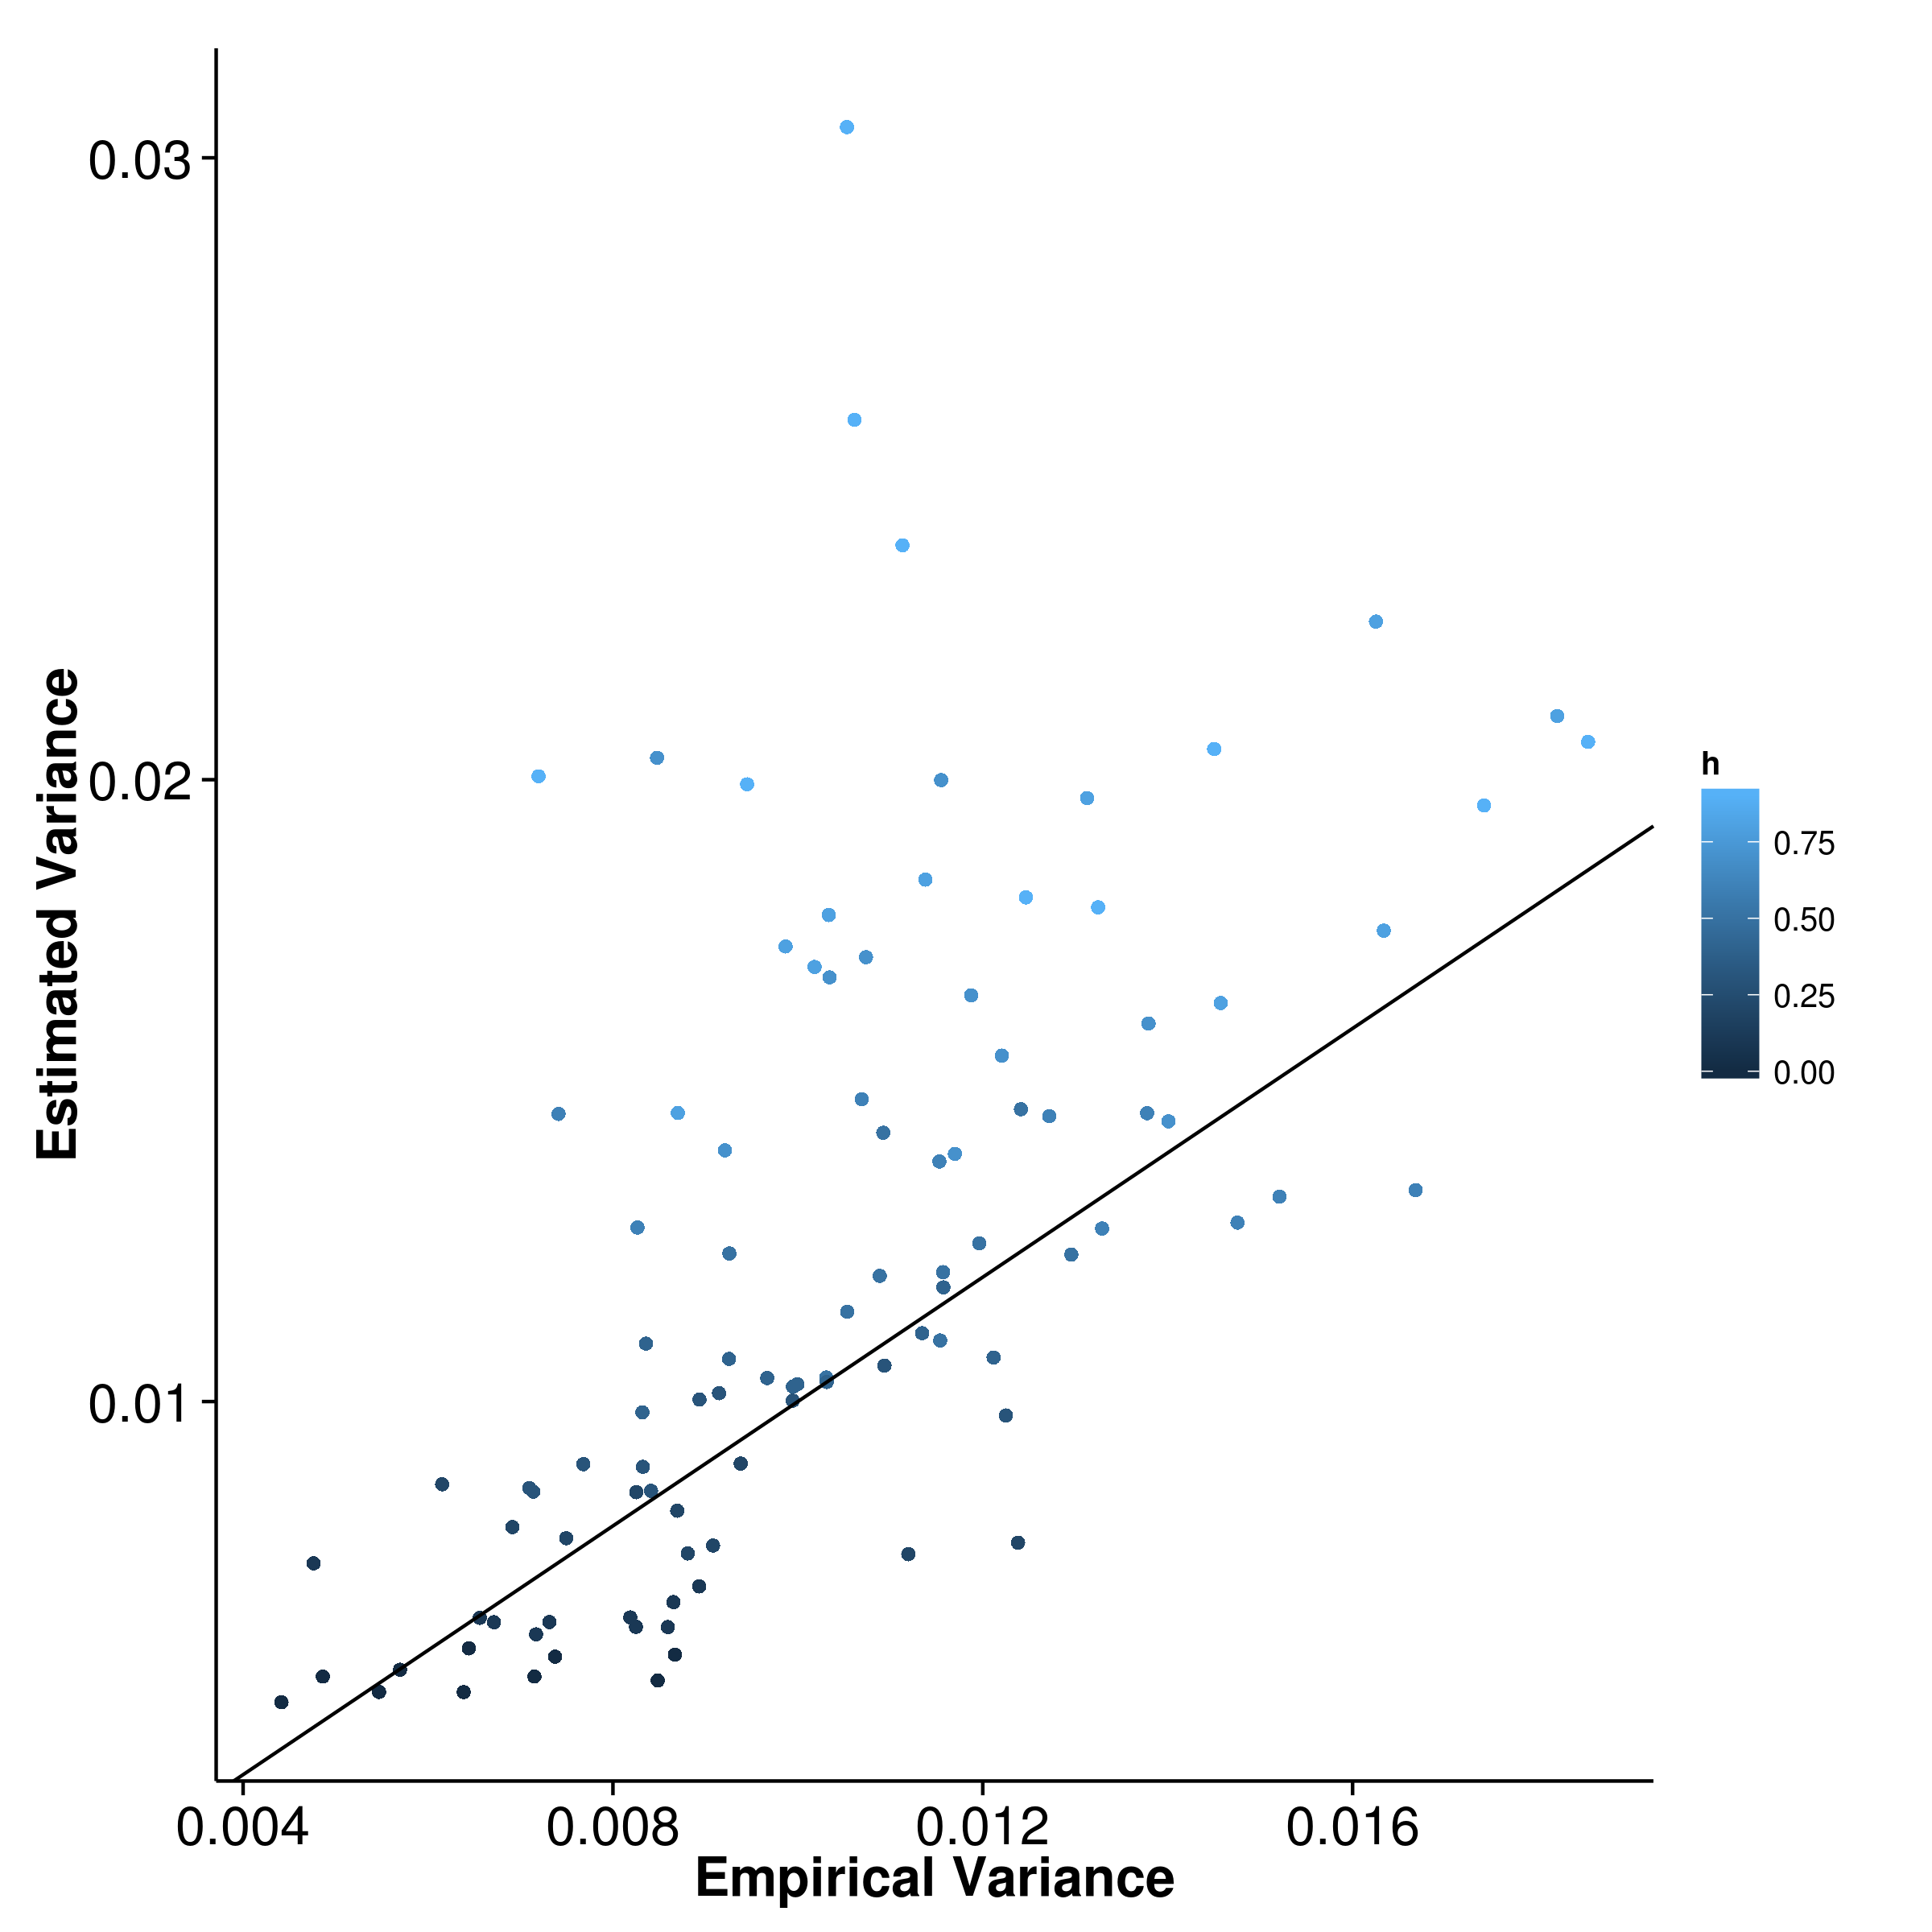
\includegraphics{figure/quantitative/same_effect/250c/ldsc_50k_250c_varH.png}}
			\label{fig:50k250cQtvarL}
		}
		\subfloat[LDSC with intercept estimation]{
			\scalebox{.4}{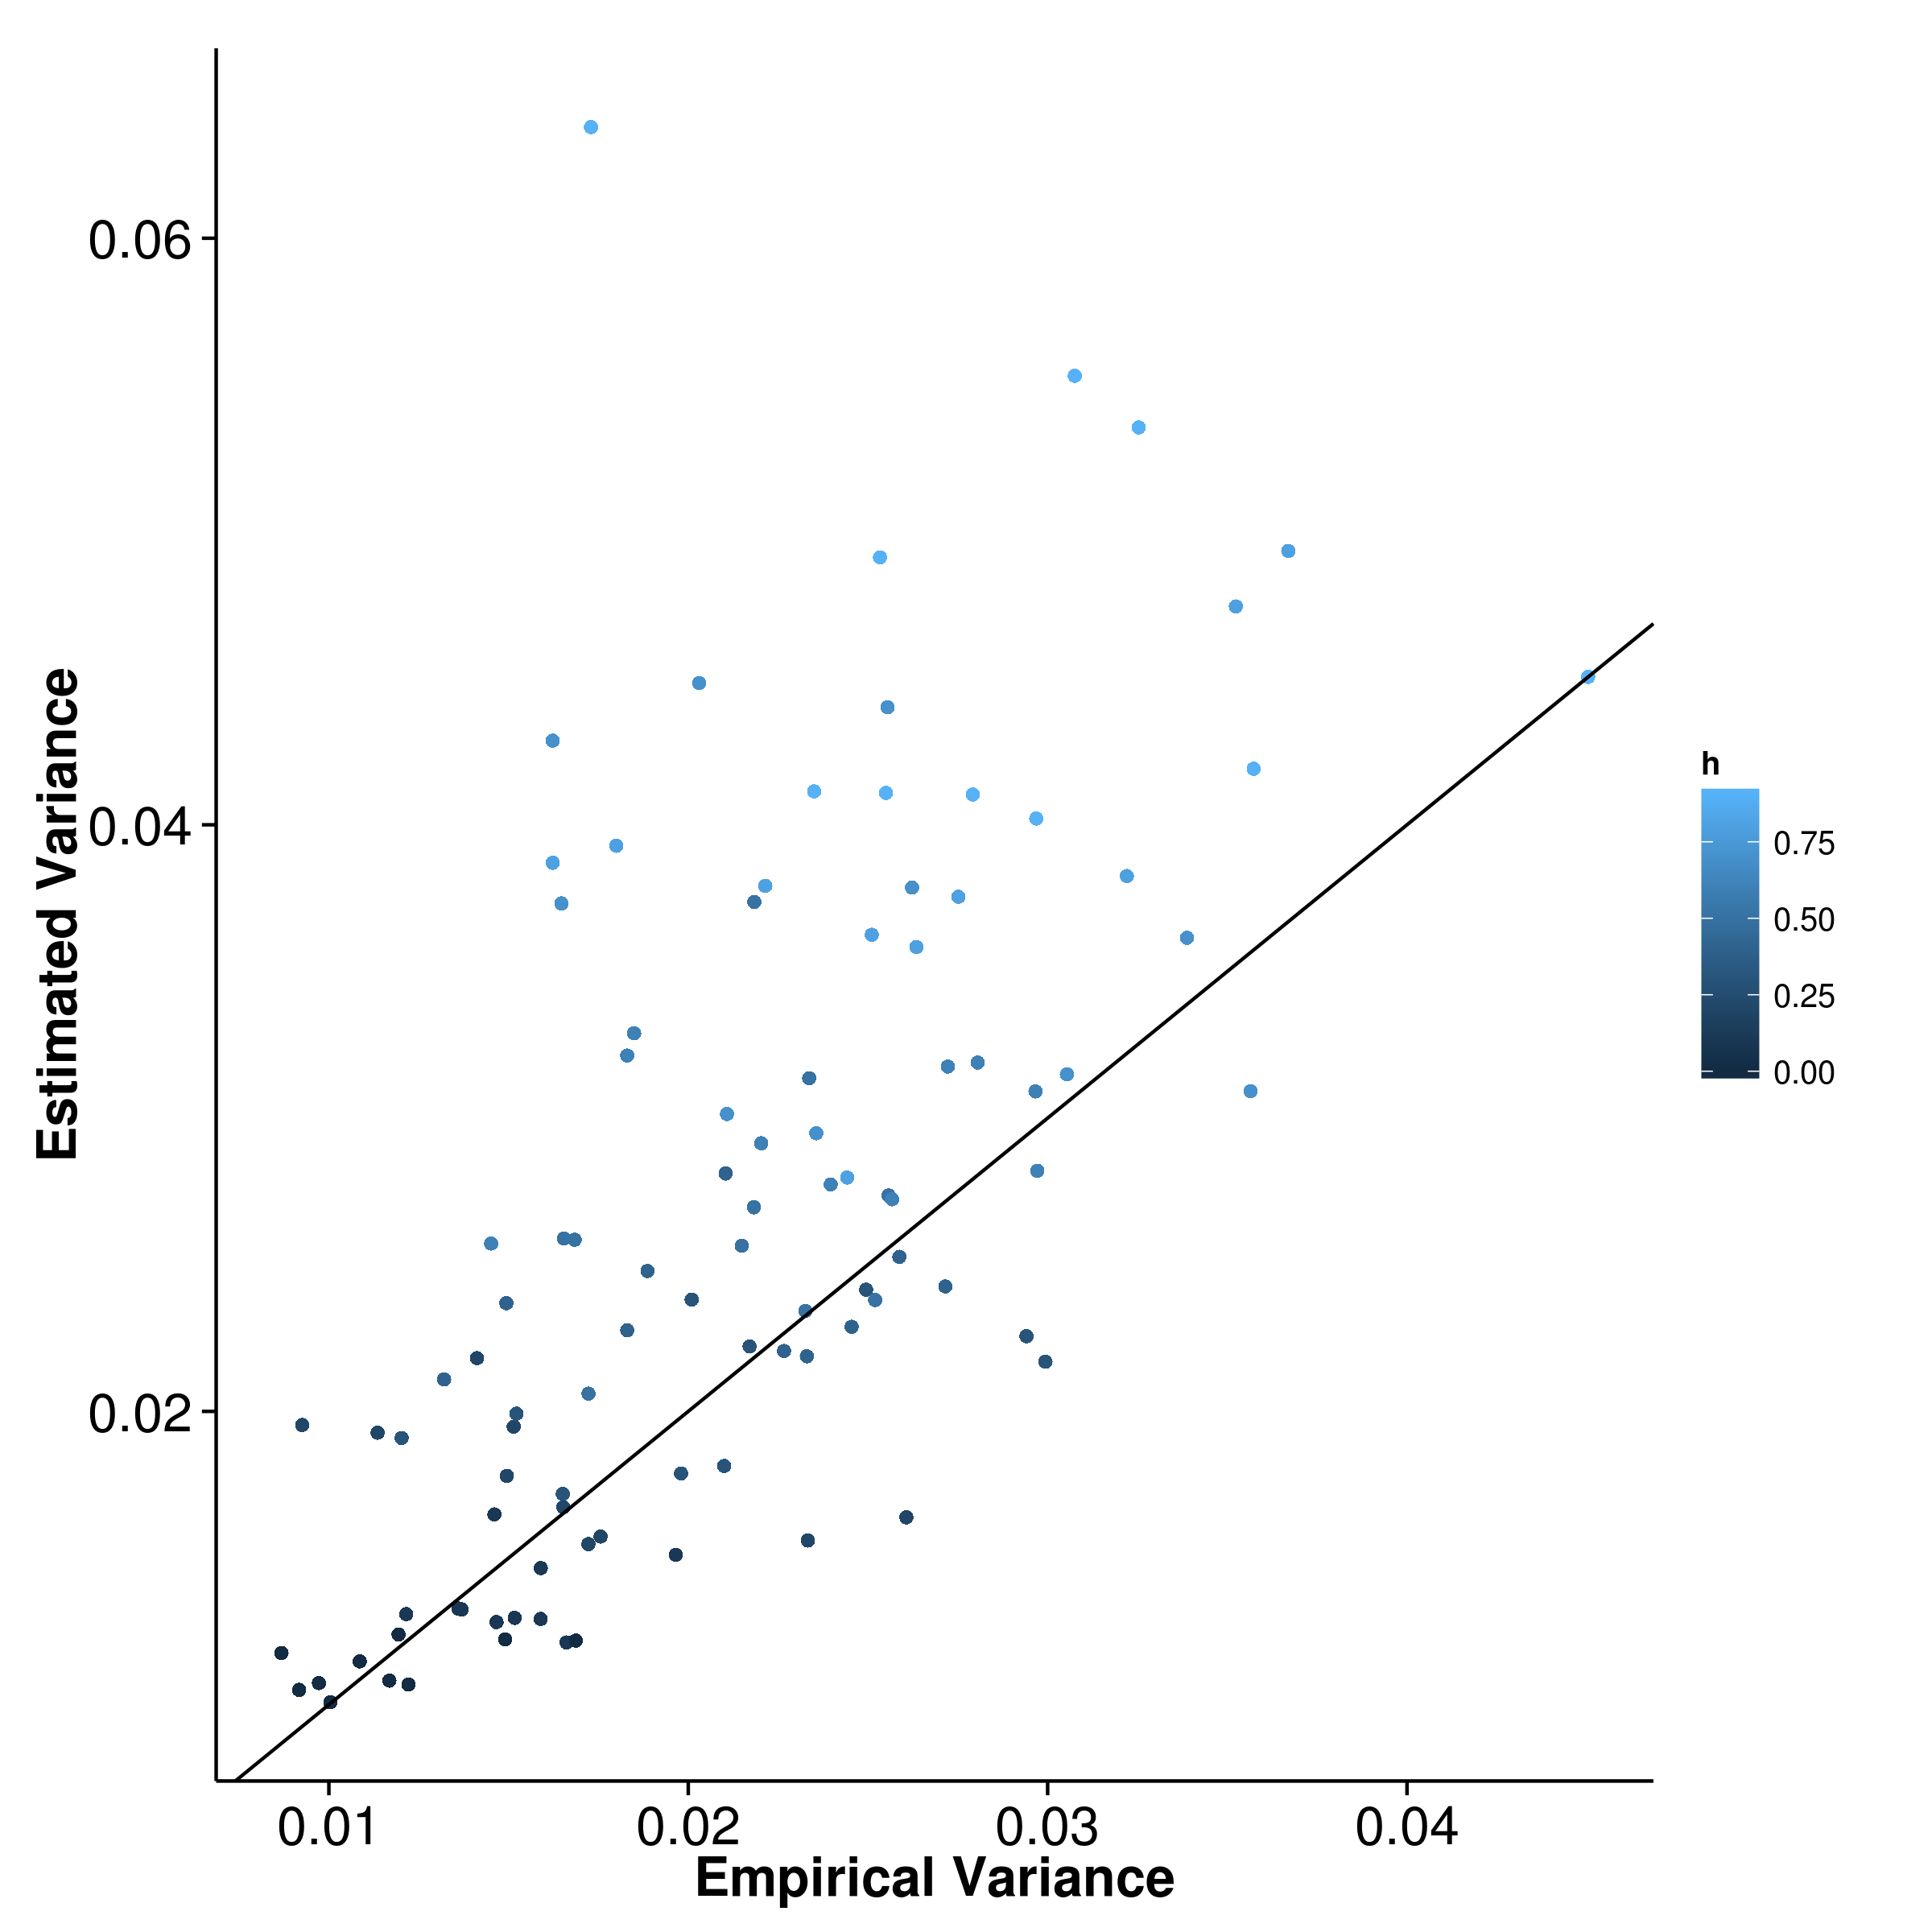
\includegraphics{figure/quantitative/same_effect/250c/ldscIn_50k_250c_varH.png}}
			\label{fig:50k250cQtvarI}
		}
		\label{fig:50k250cQtVar}
	\end{figure}
	
	
	
	\begin{figure}
		\centering
		\subfloat[SHREK]{
			\scalebox{.4}{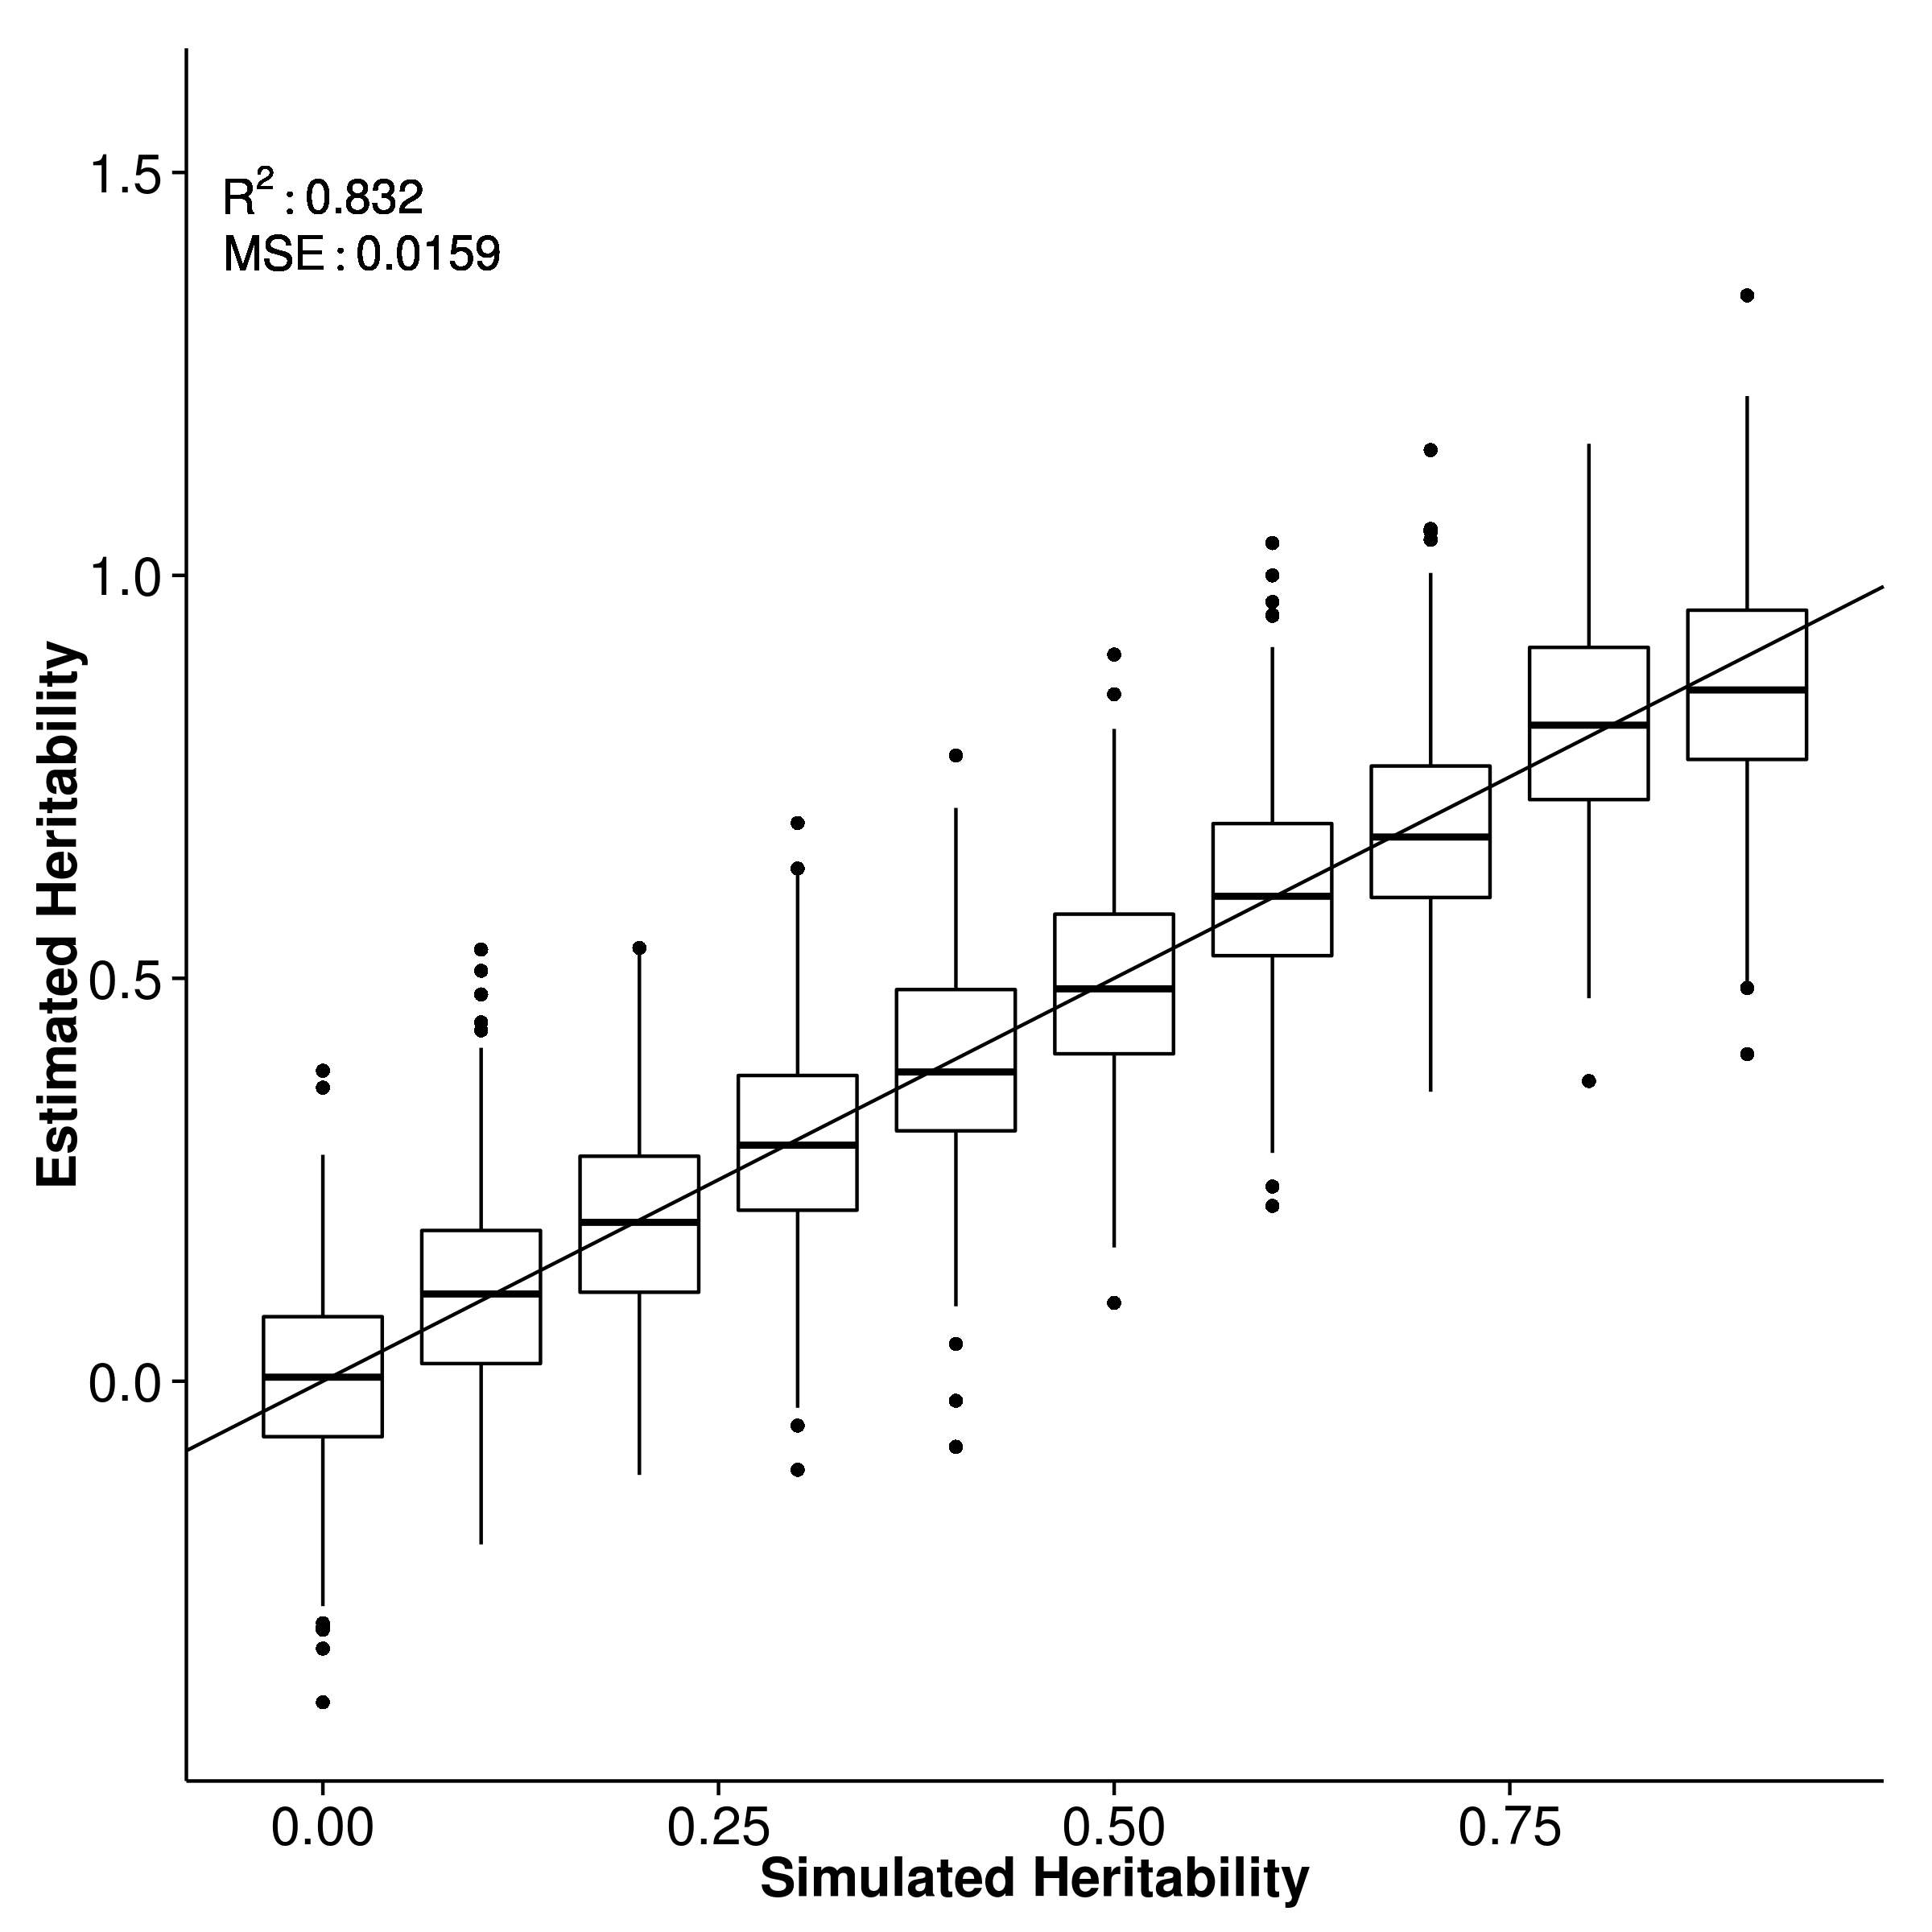
\includegraphics{figure/quantitative/random_effect/10c/shrek_50k_10c_meanH.png}}
			\label{fig:50k10cQtmeanSre}
		}
		\subfloat[GCTA]{
			\scalebox{.4}{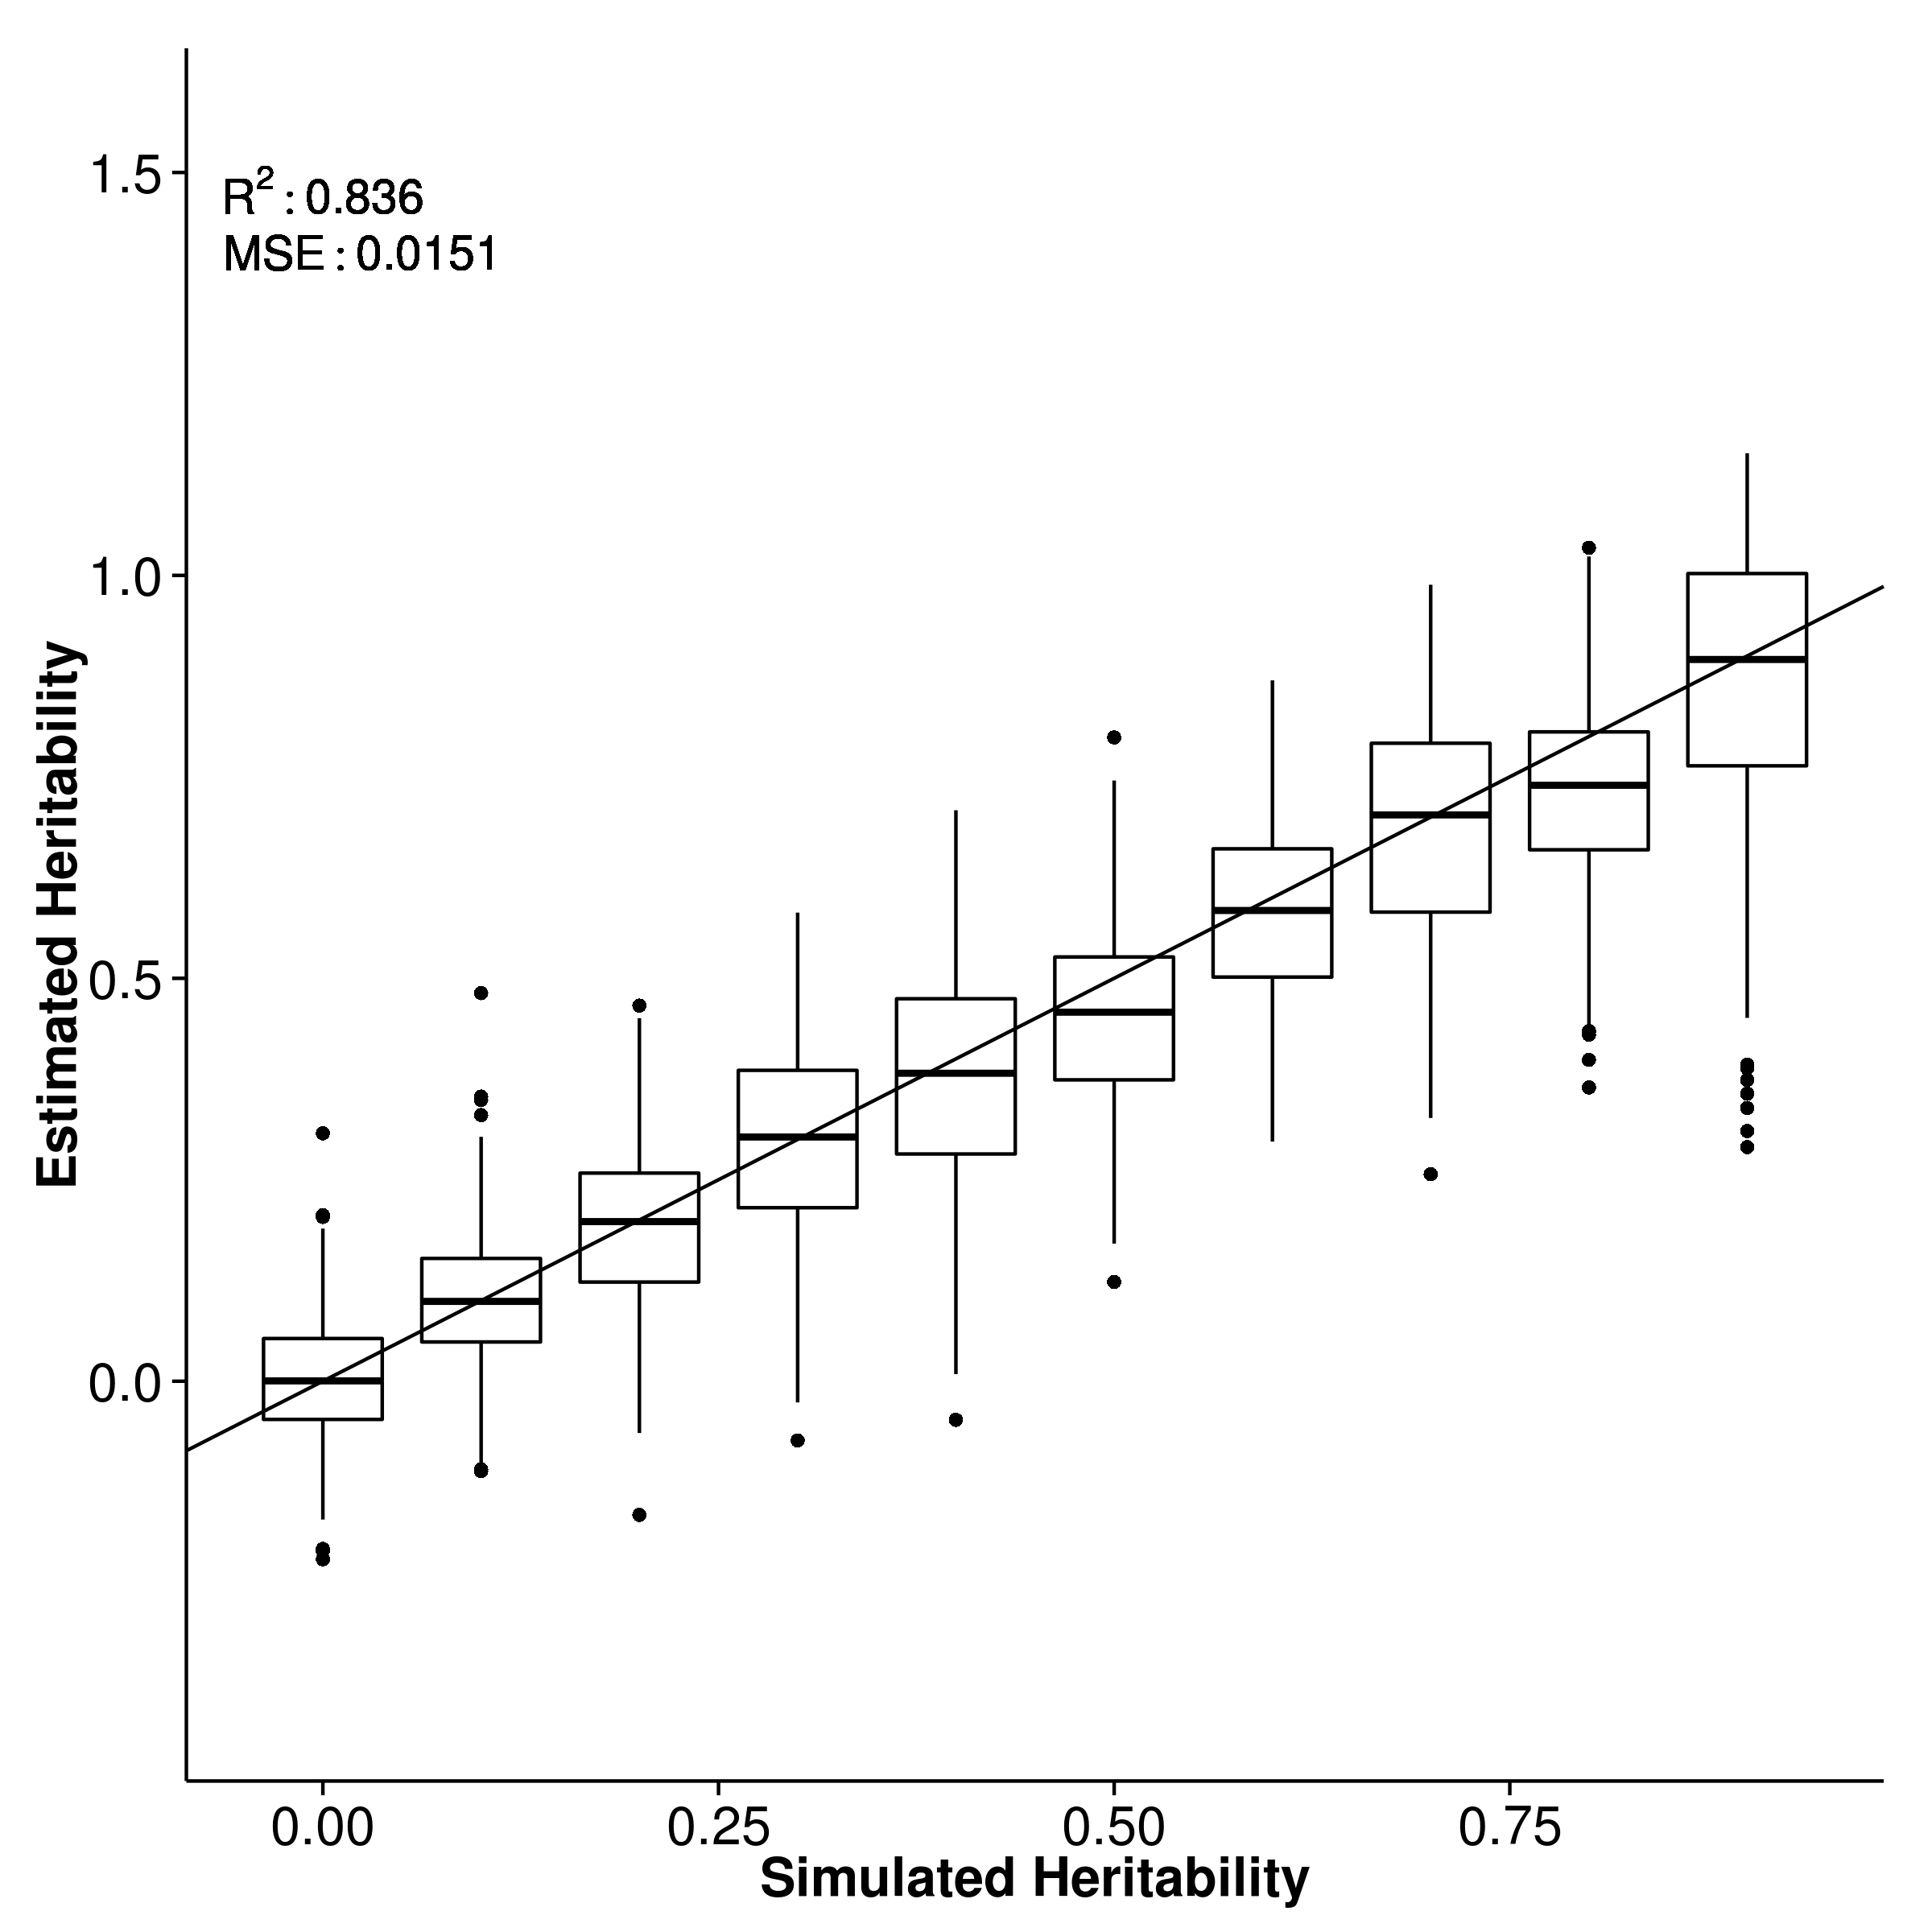
\includegraphics{figure/quantitative/random_effect/10c/gcta_50k_10c_meanH.png}}
			\label{fig:50k10cQtmeanGre}
		}\\
		\subfloat[LDSC with fix intercept]{
			\scalebox{.4}{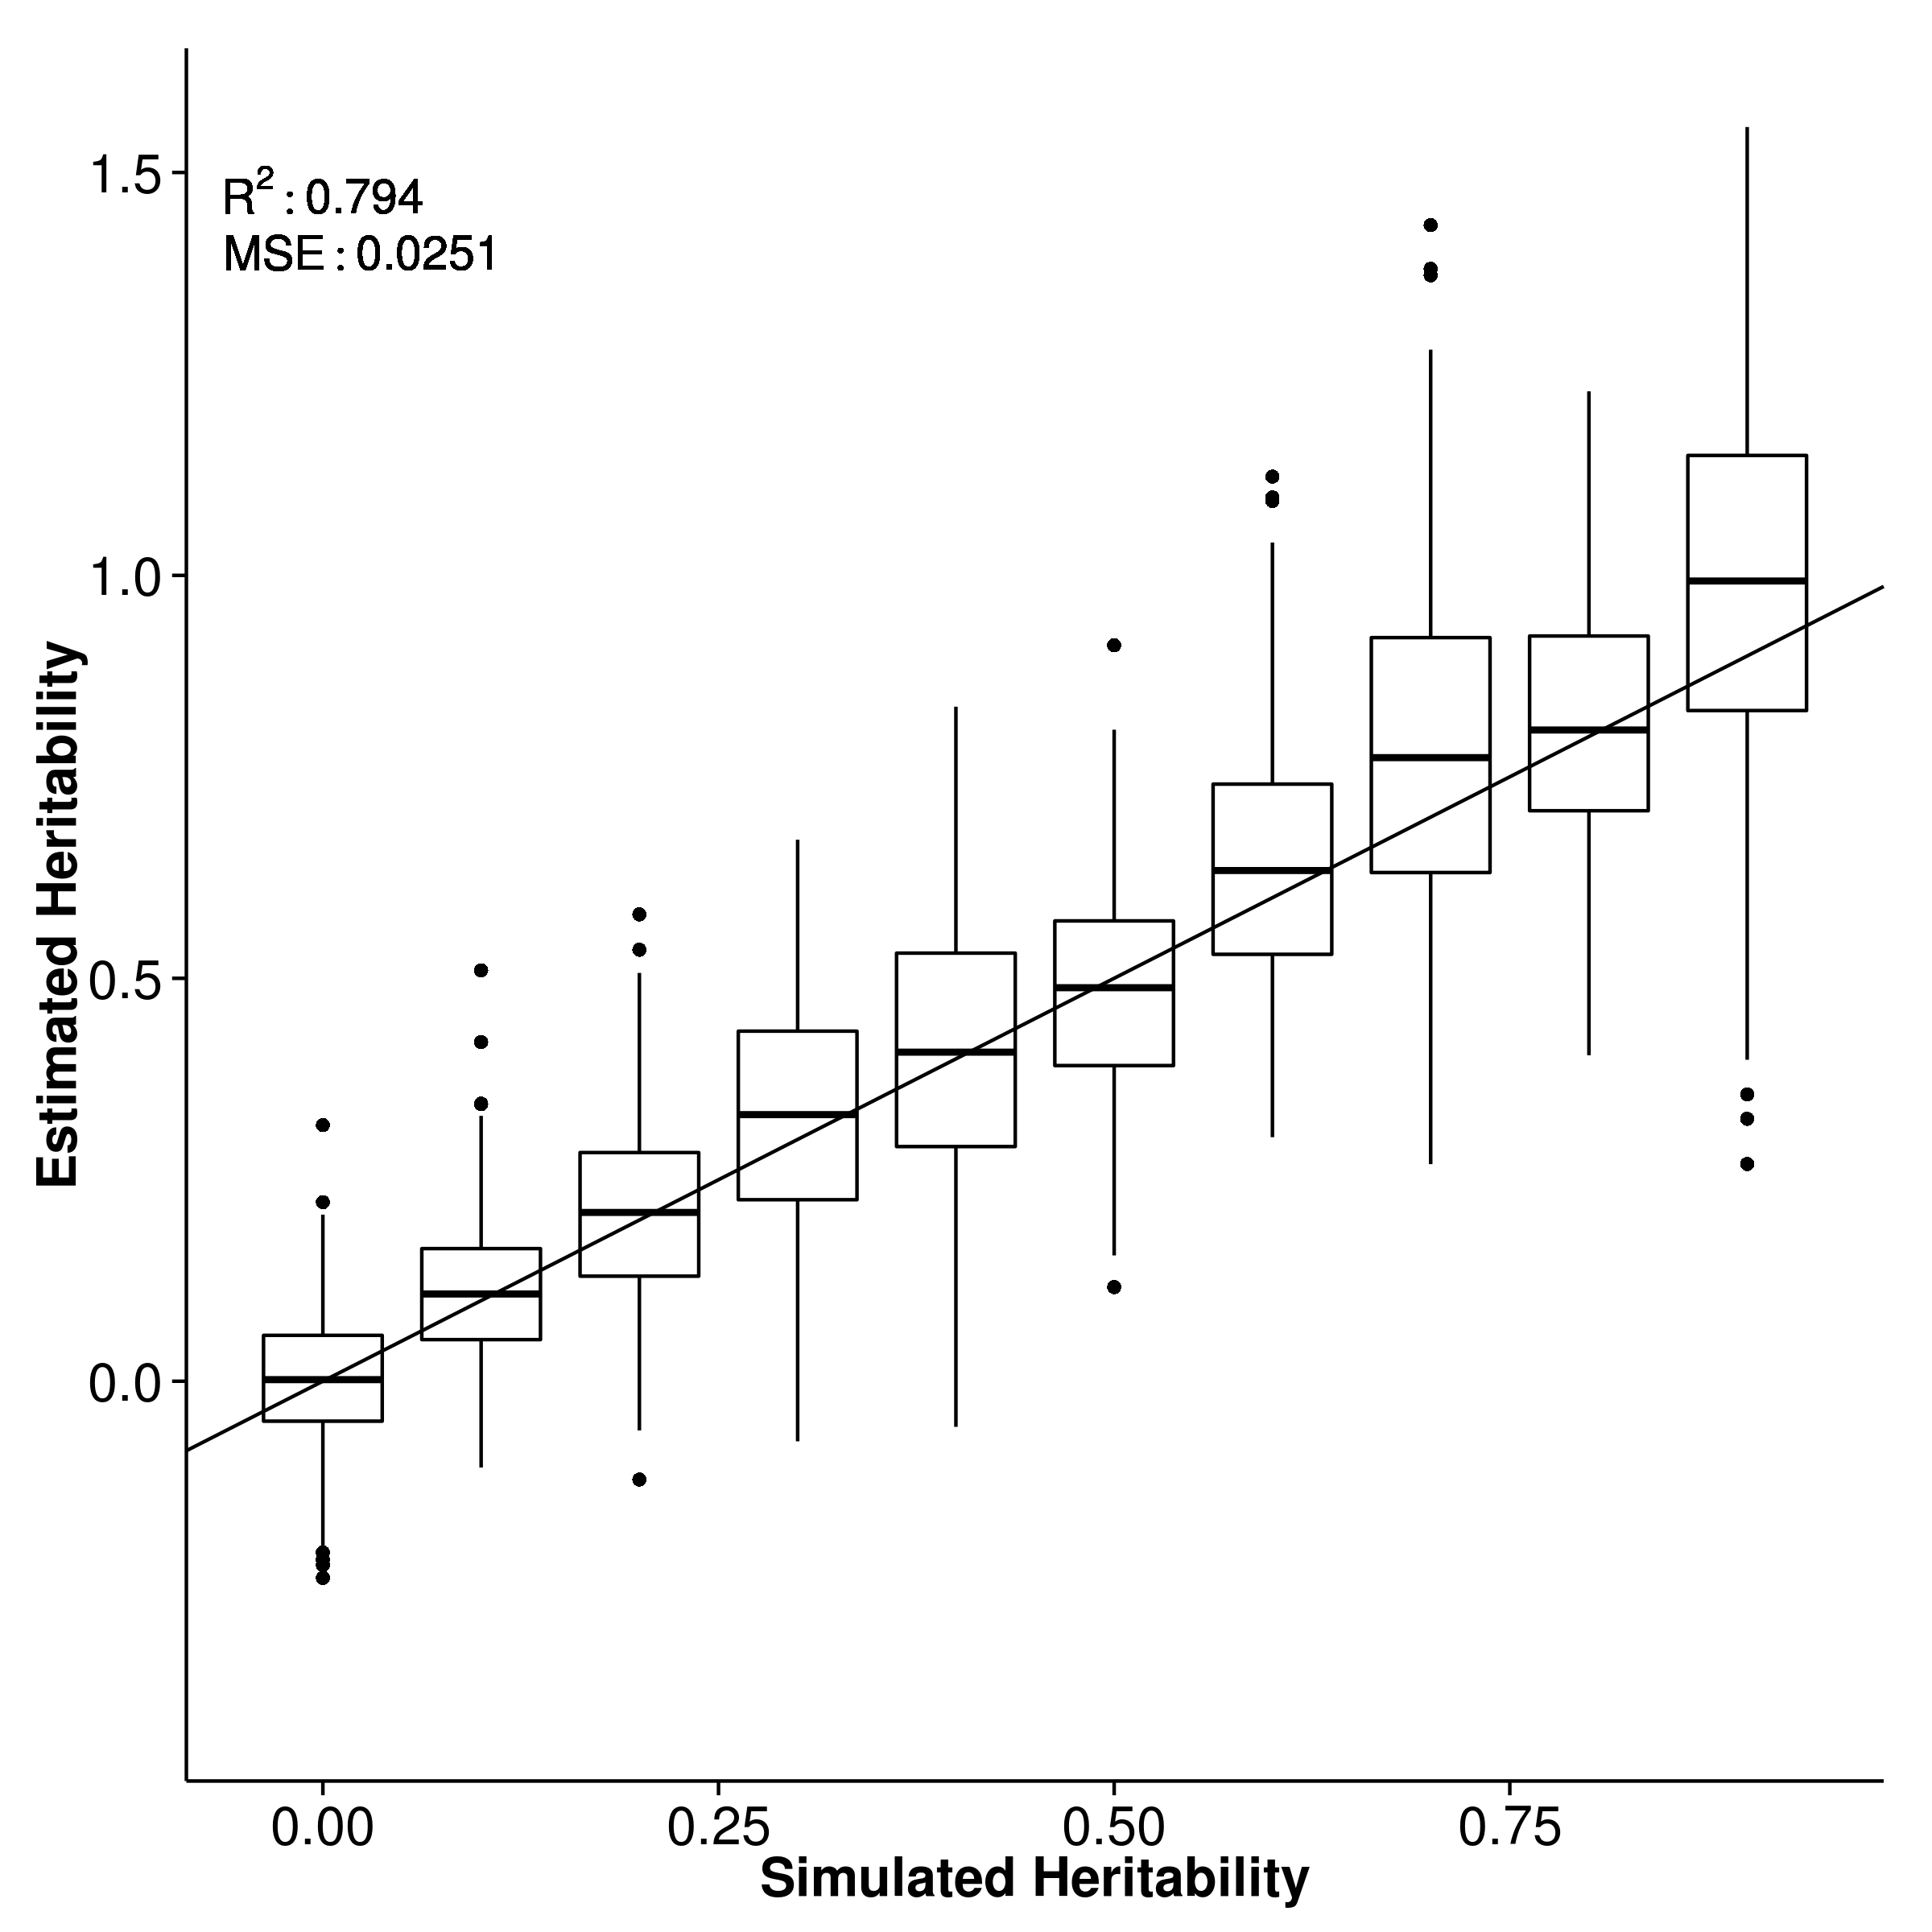
\includegraphics{figure/quantitative/random_effect/10c/ldsc_50k_10c_meanH.png}}
			\label{fig:50k10cQtmeanLre}
		}
		\subfloat[LDSC with intercept estimation]{
			\scalebox{.4}{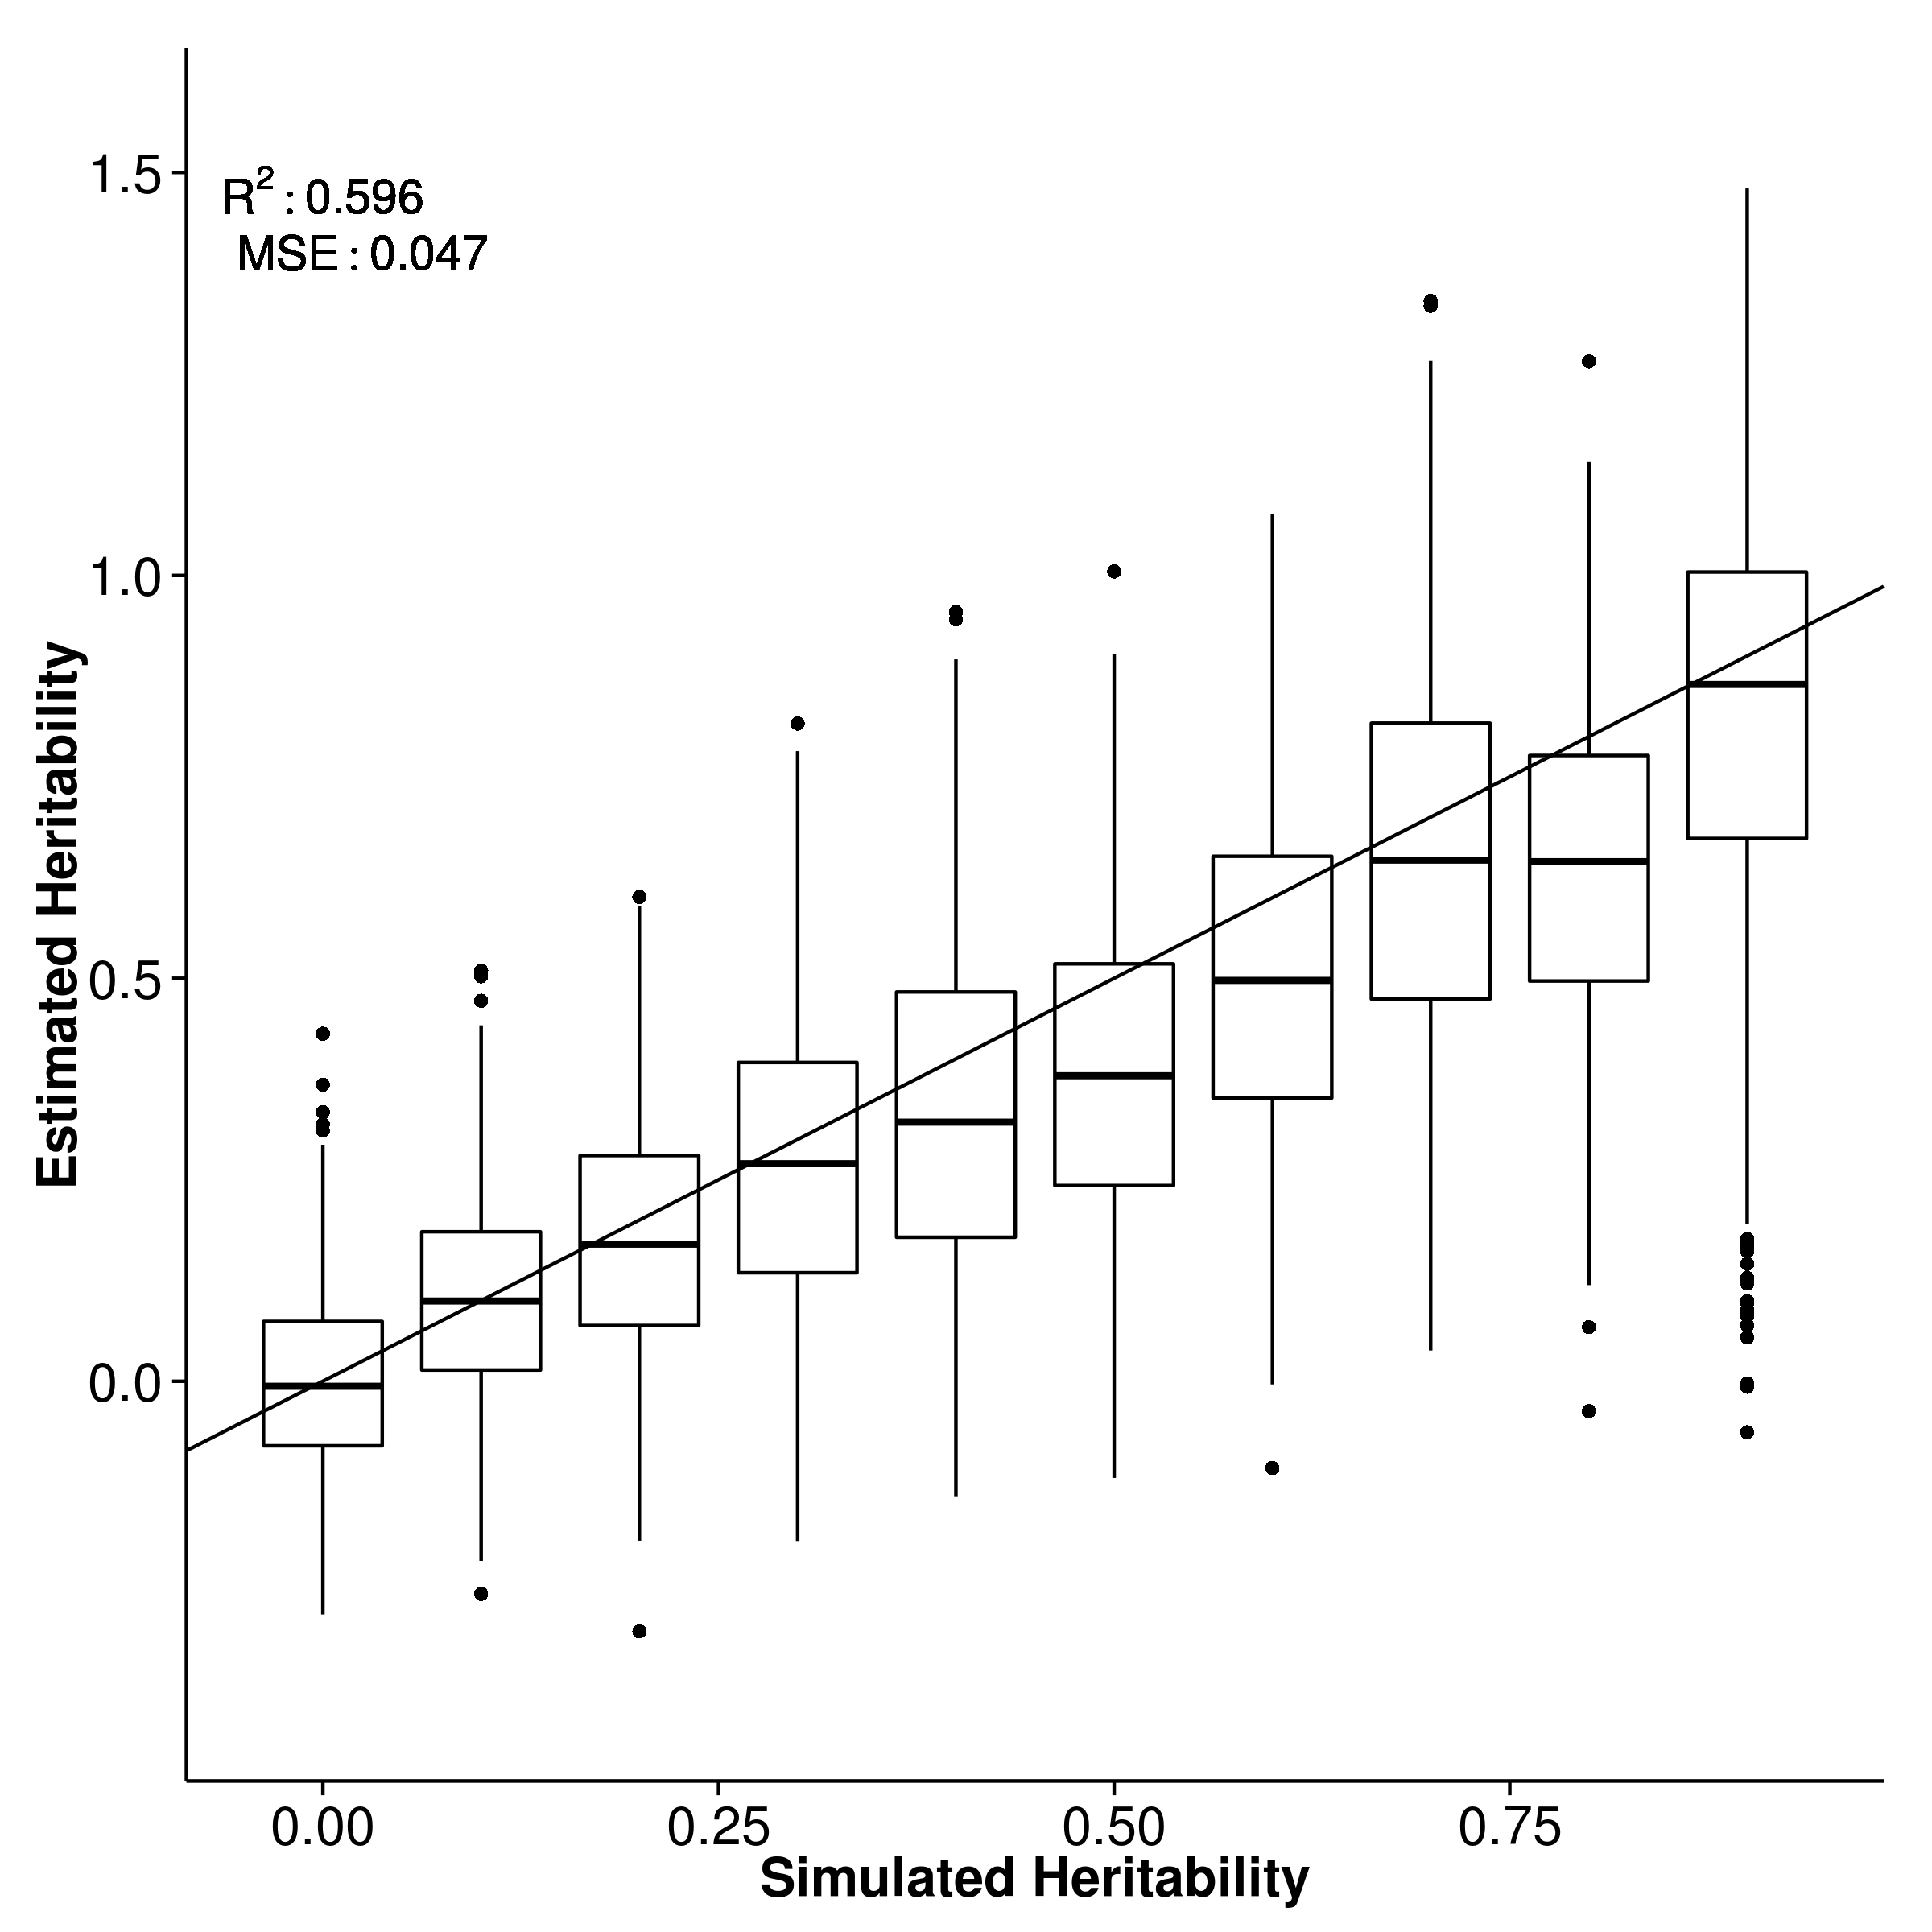
\includegraphics{figure/quantitative/random_effect/10c/ldscIn_50k_10c_meanH.png}}
			\label{fig:50k10cQtmeanIre}
		}
		\caption[Simulation of Quantitative Traits with 50k \glsentryshortpl{SNP} and 10 causal variants of random effect size]
		{Simulation of Quantitative Traits with 50k \glsentryshortpl{SNP} and 10 causal variants with random effect size.} 
		\label{fig:50k10cQtMeanre}
	\end{figure}
	\begin{figure}
		\centering
		\subfloat[SHREK]{
			\scalebox{.4}{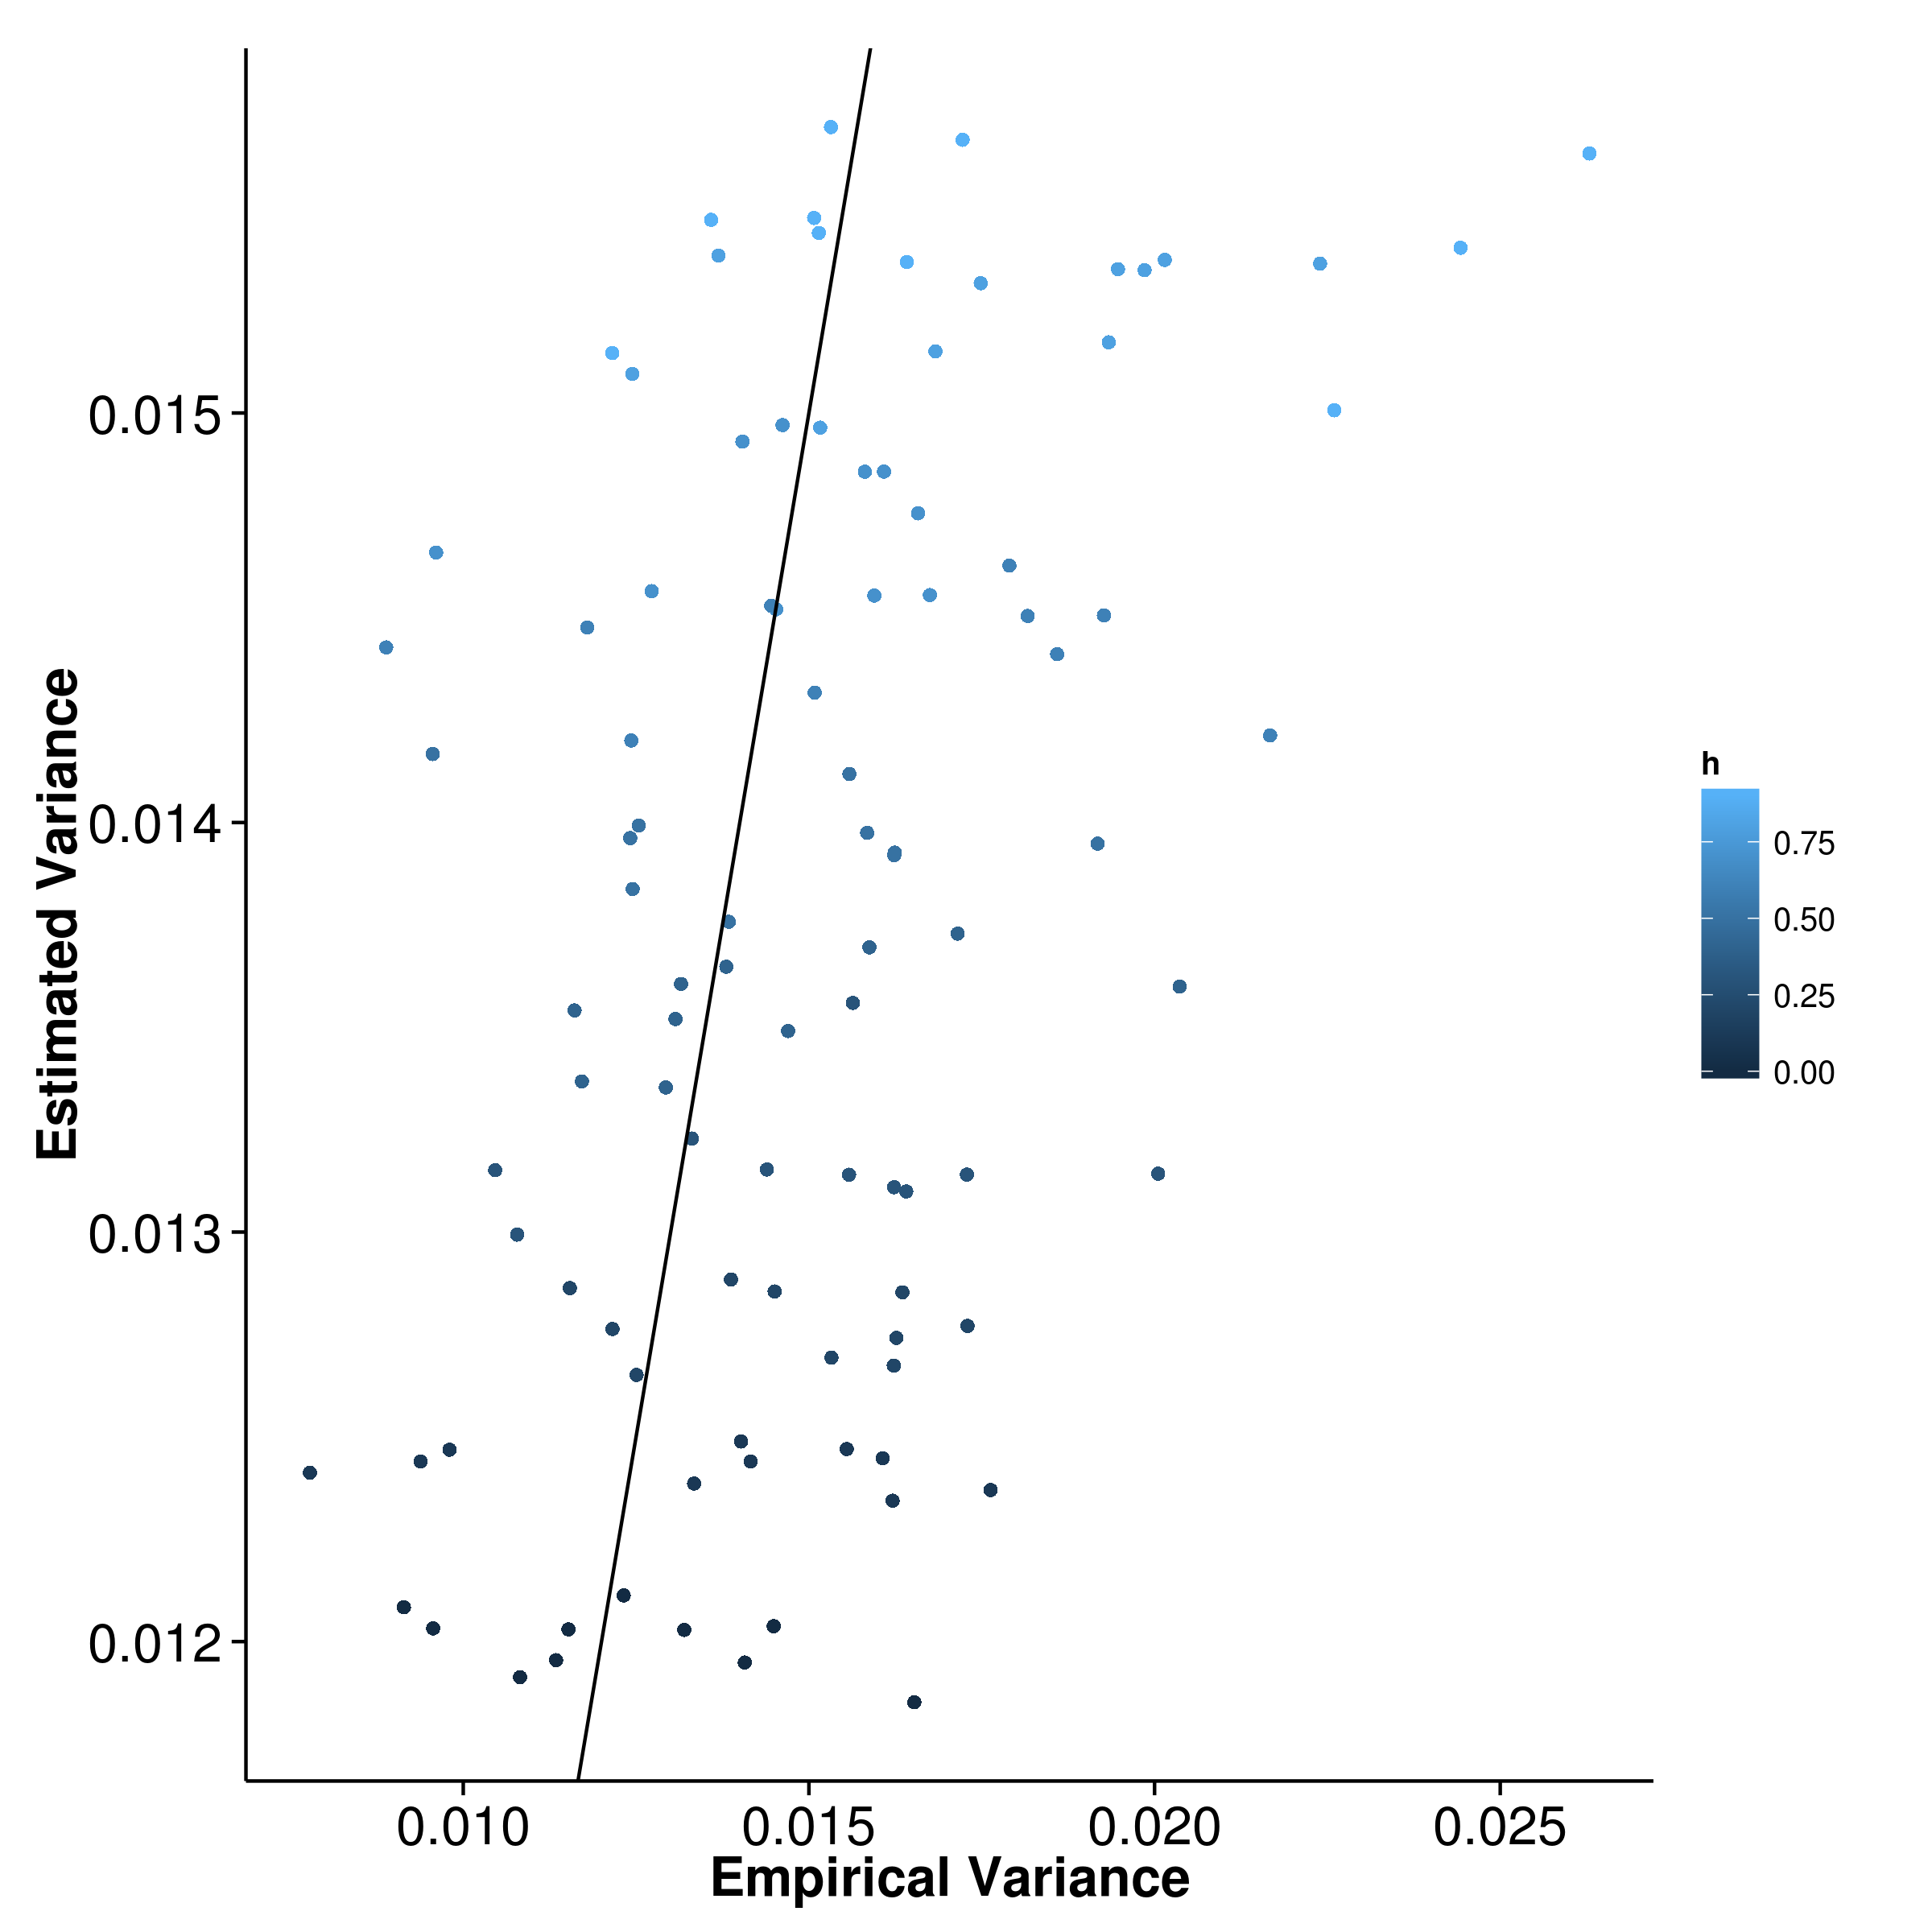
\includegraphics{figure/quantitative/random_effect/10c/shrek_50k_10c_varH.png}}
			\label{fig:50k10cQtvarSre}
		}
		\subfloat[GCTA]{
			\scalebox{.4}{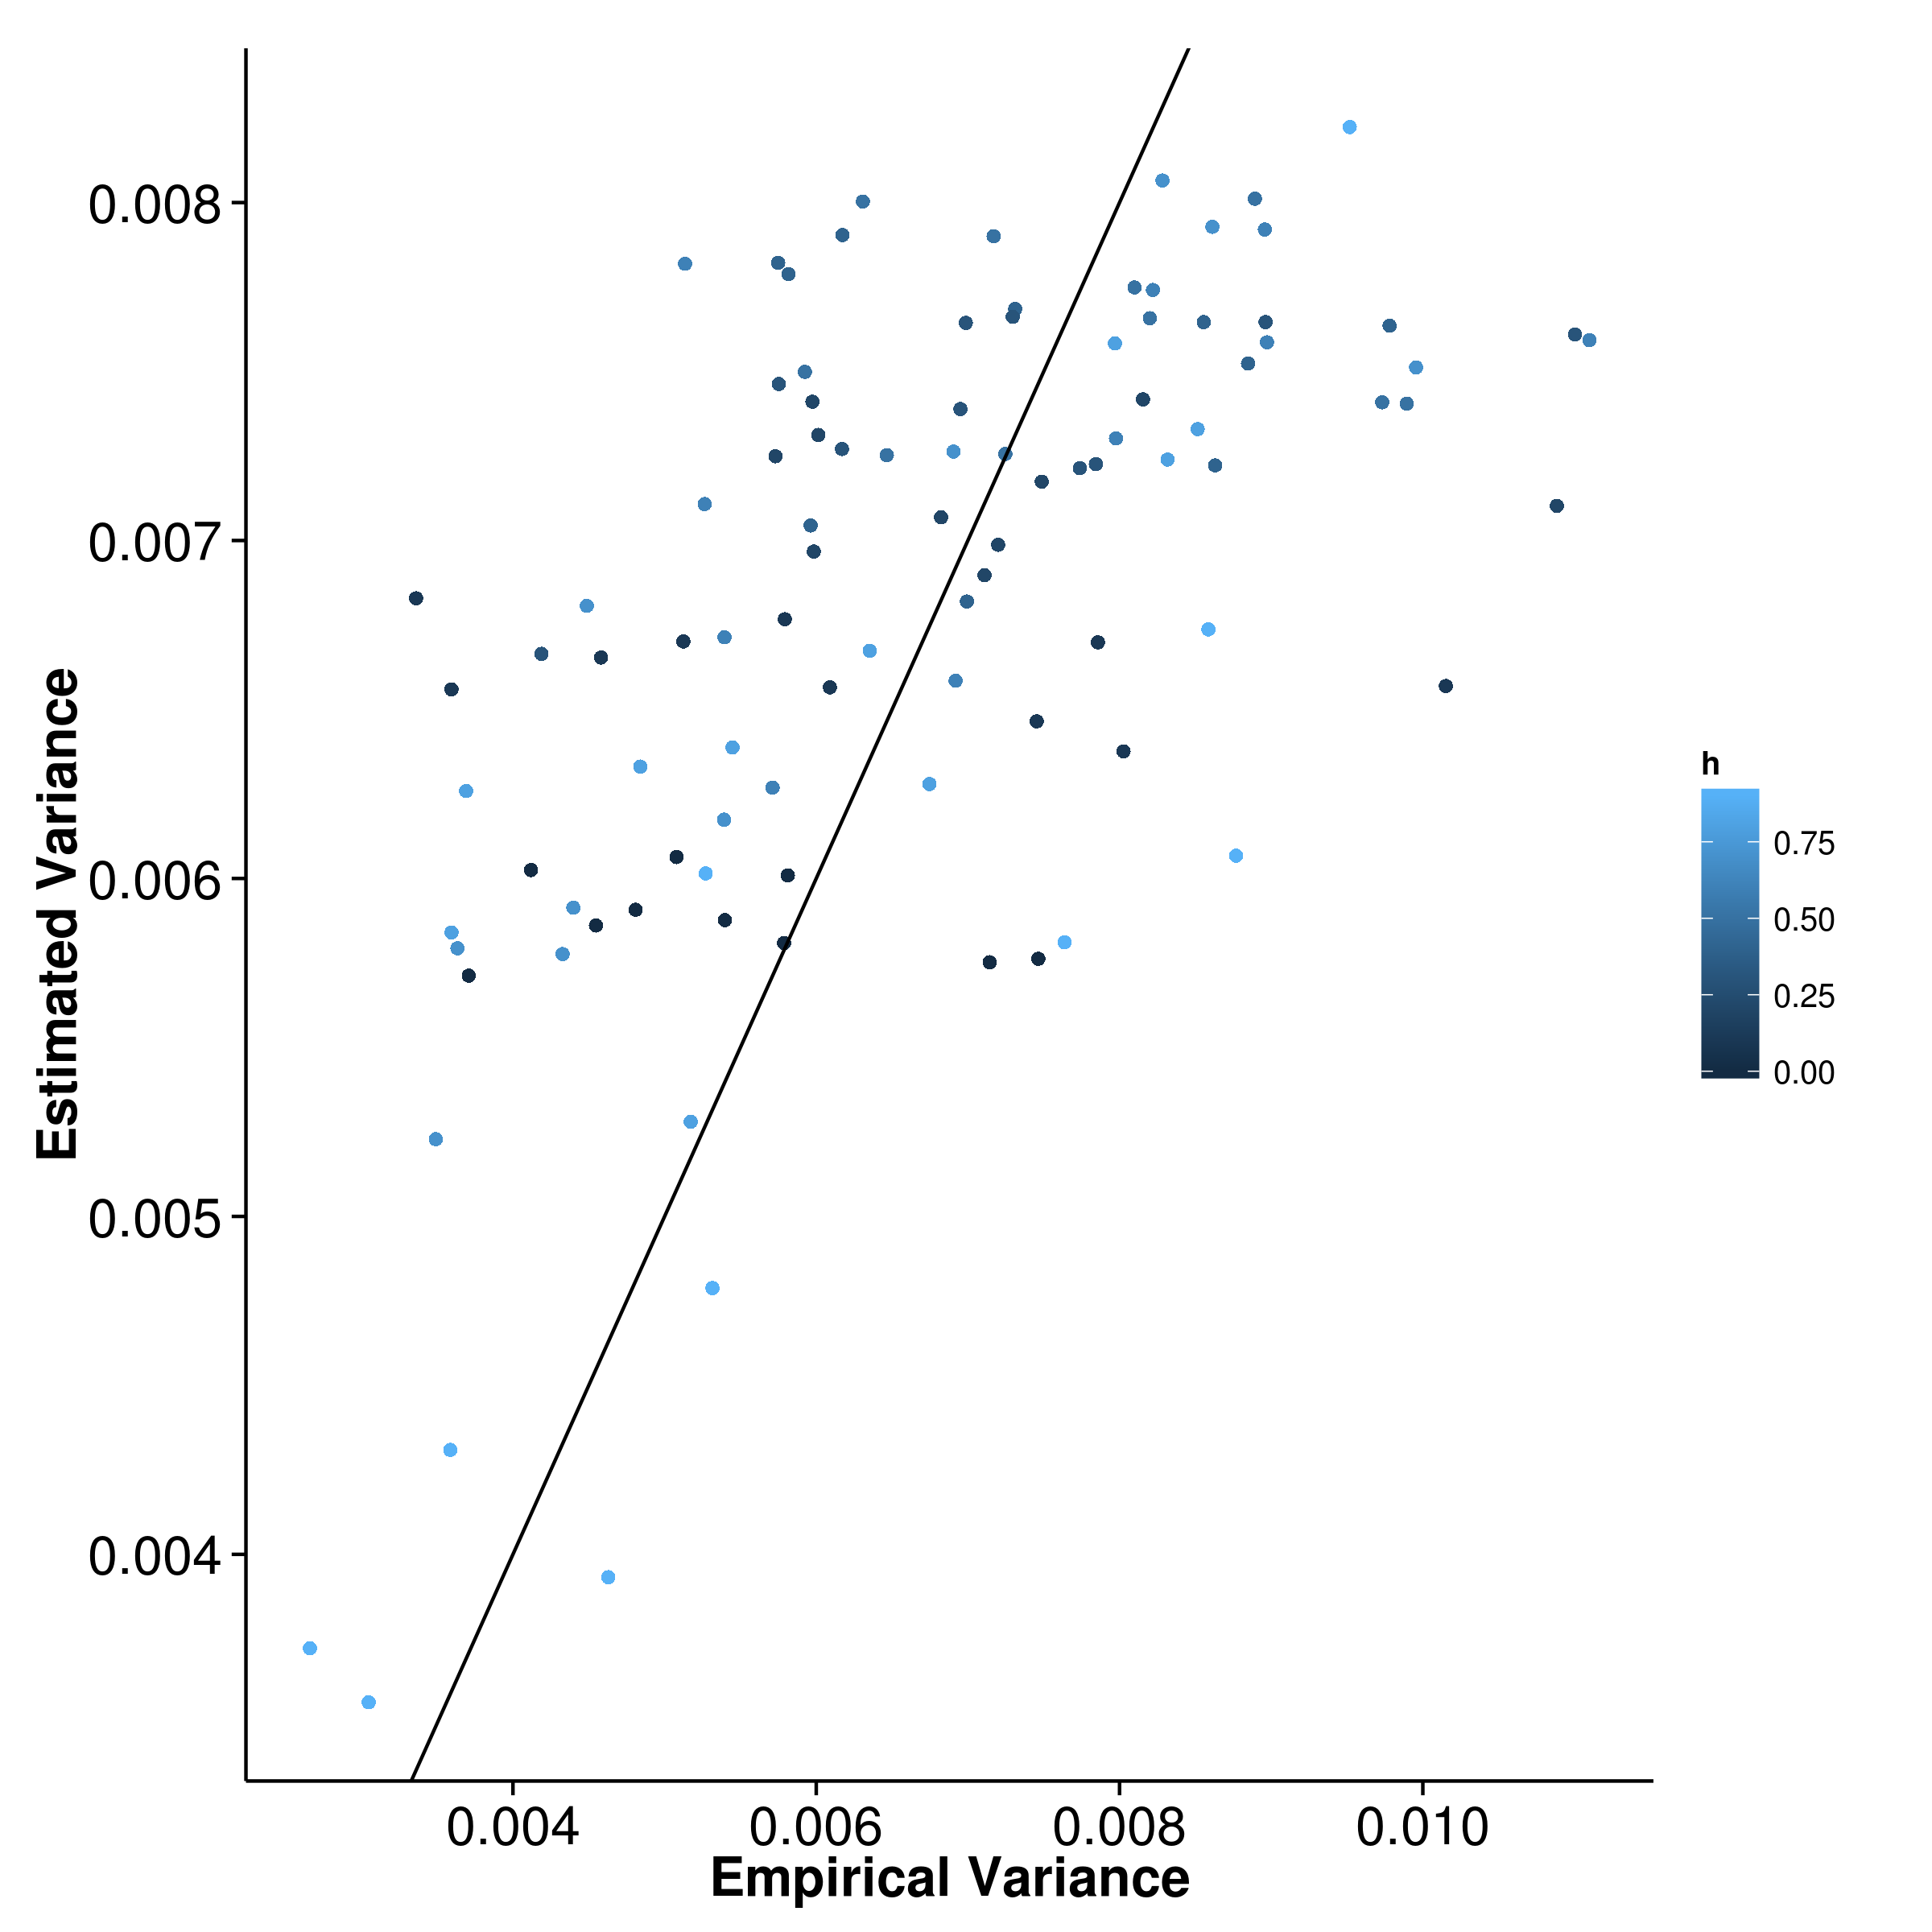
\includegraphics{figure/quantitative/random_effect/10c/gcta_50k_10c_varH.png}}
			\label{fig:50k10cQtvarGre}
		}\\
		\subfloat[LDSC with fix intercept]{
			\scalebox{.4}{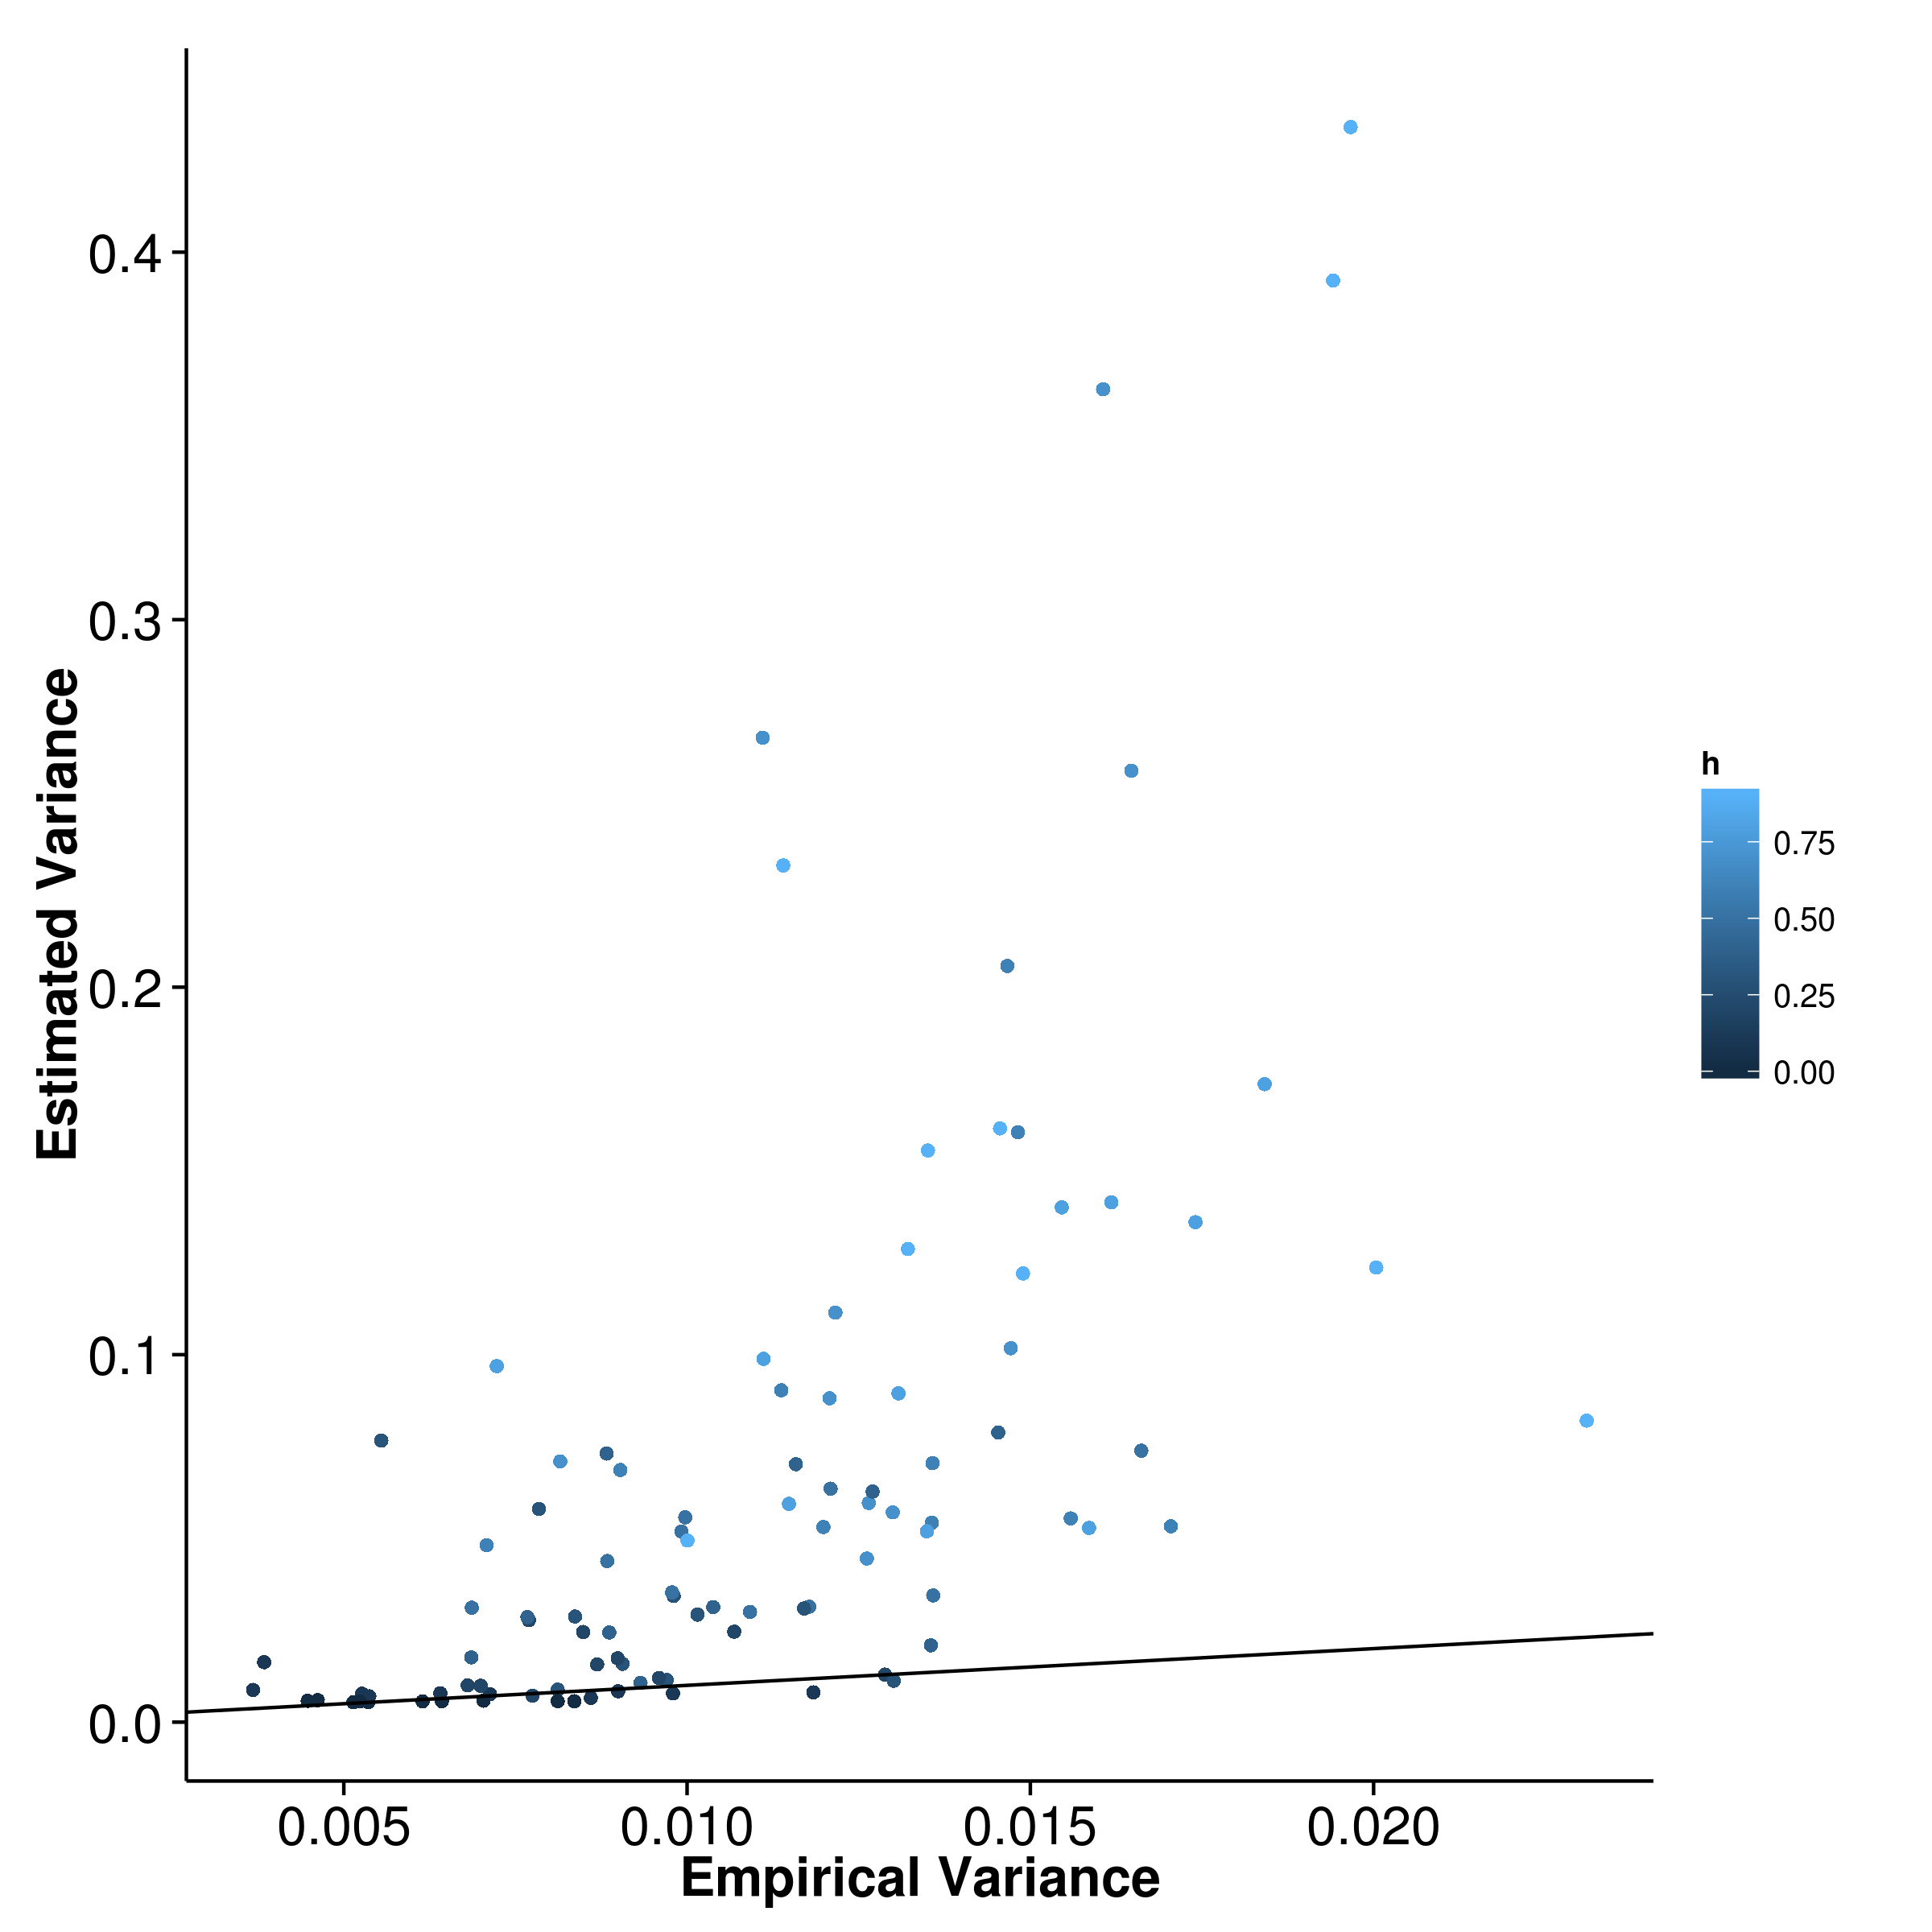
\includegraphics{figure/quantitative/random_effect/10c/ldsc_50k_10c_varH.png}}
			\label{fig:50k10cQtvarLre}
		}
		\subfloat[LDSC with intercept estimation]{
			\scalebox{.4}{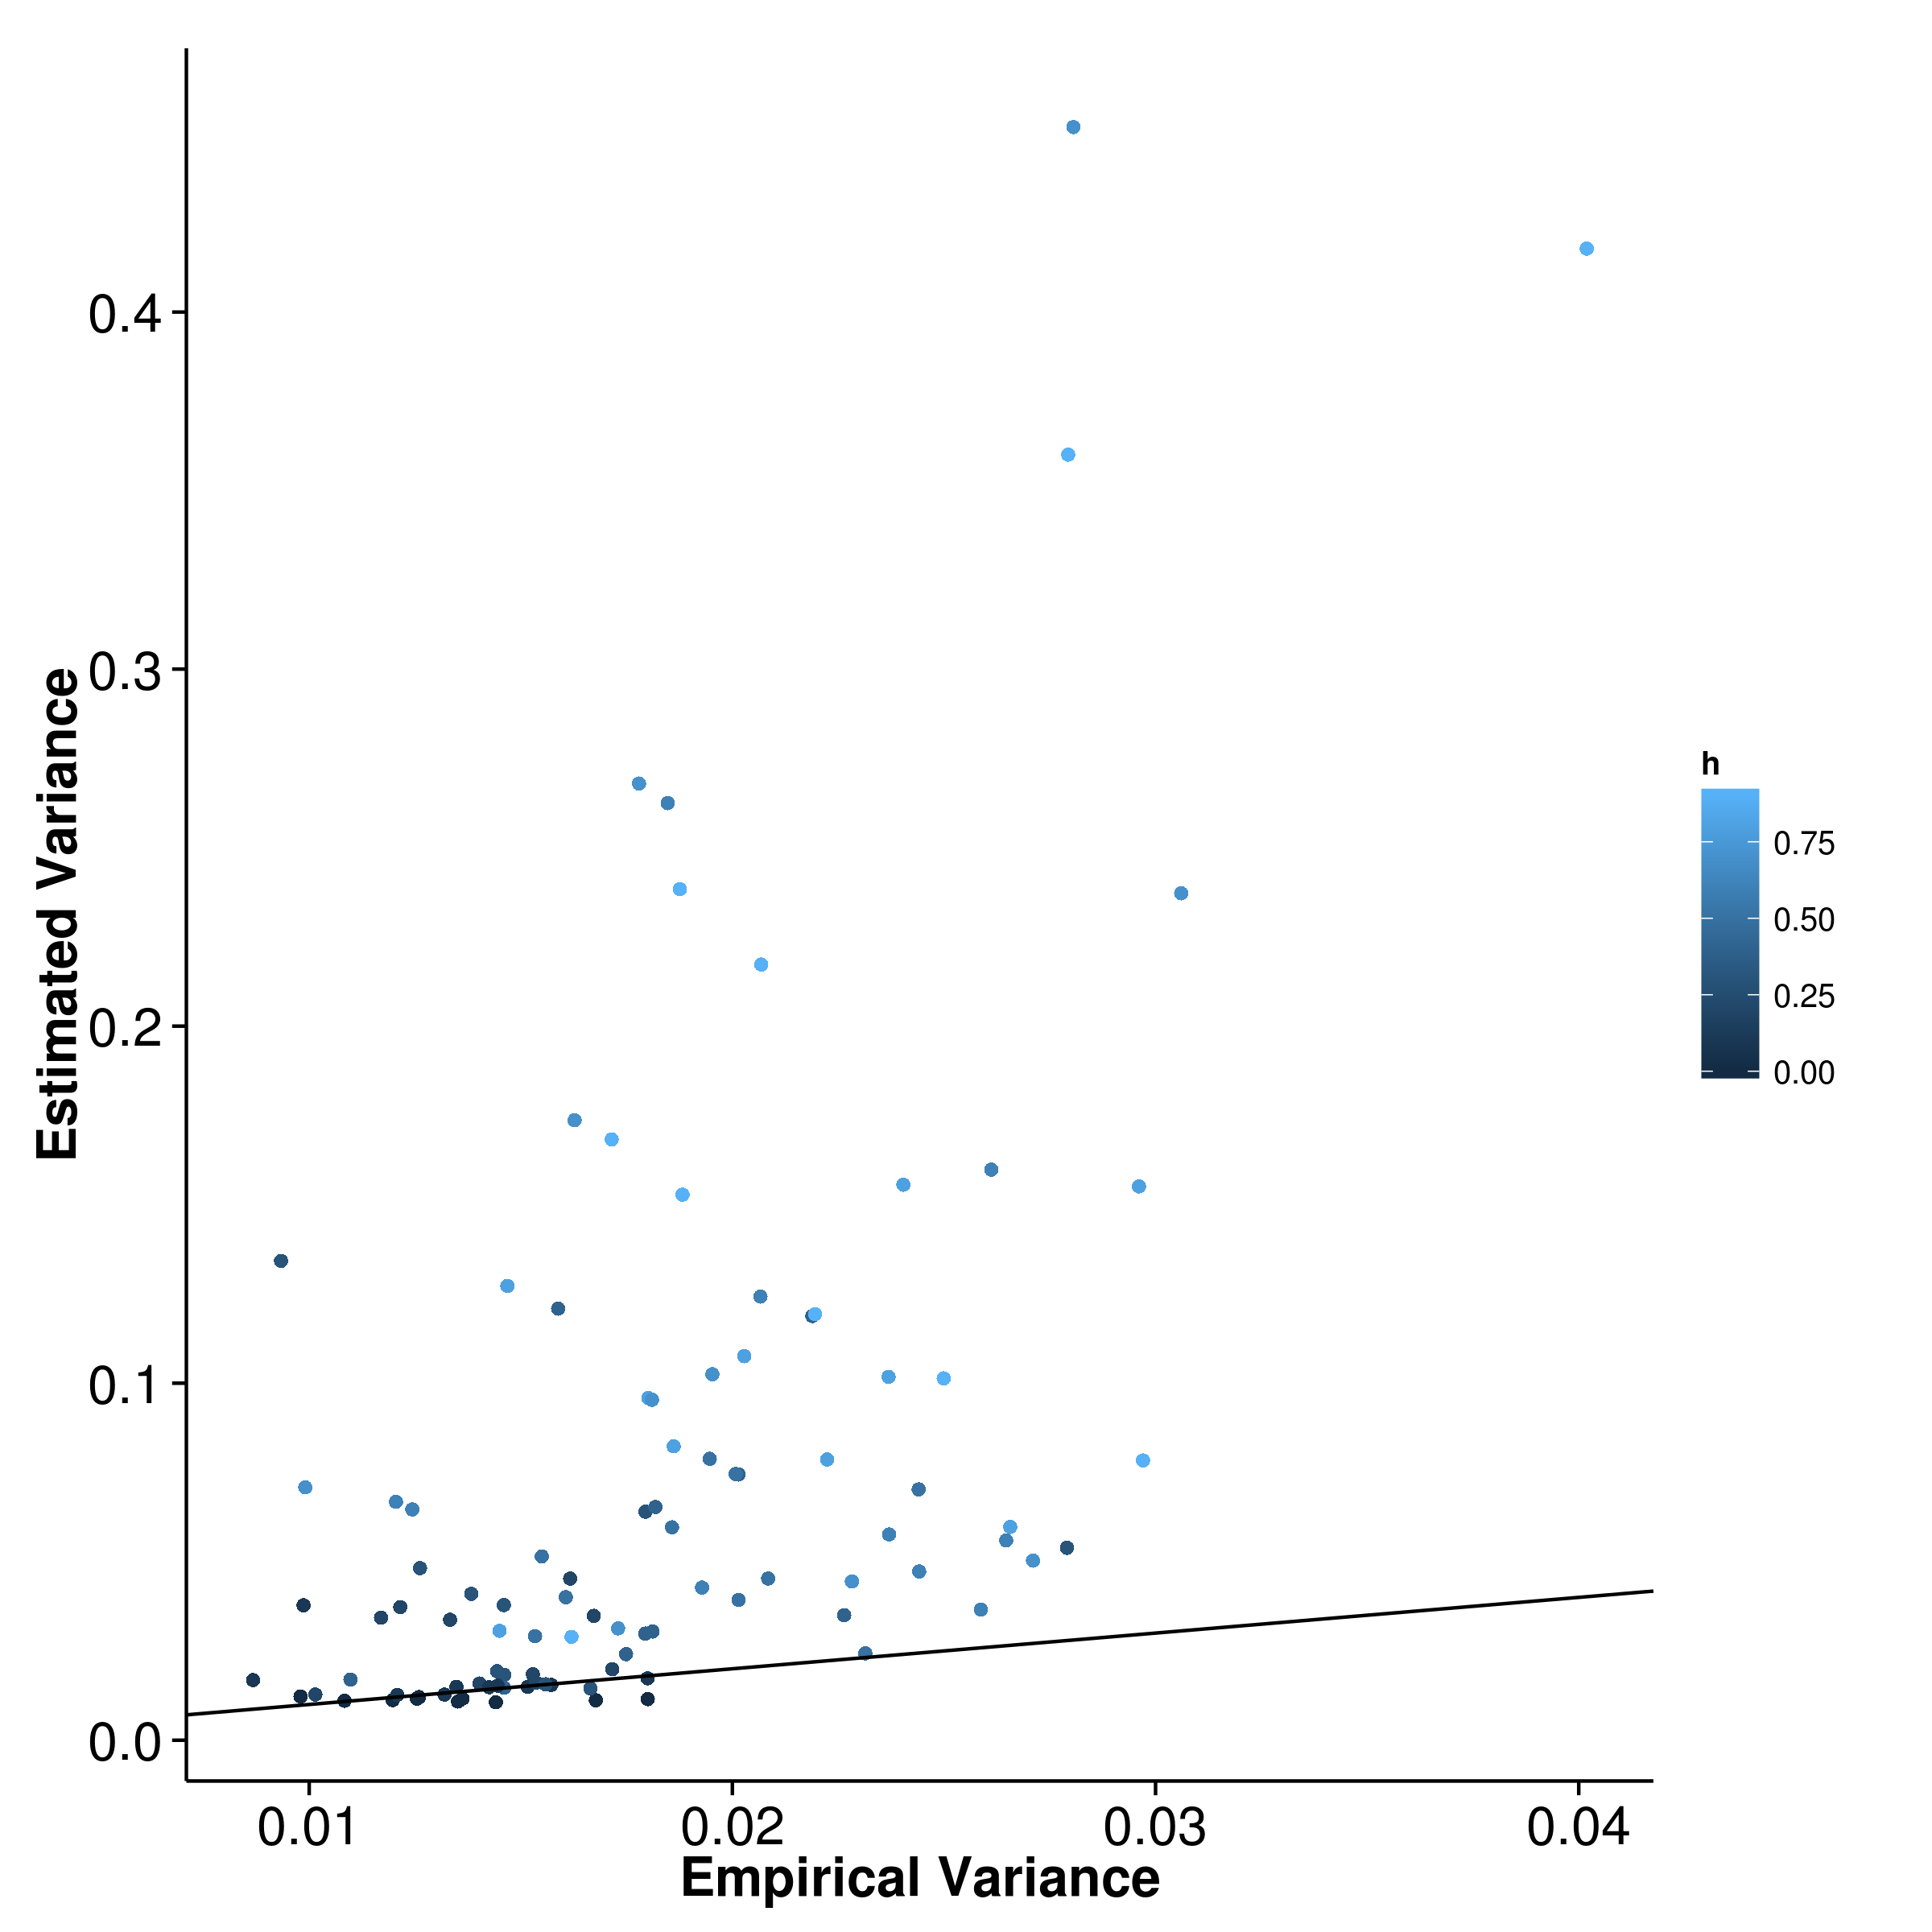
\includegraphics{figure/quantitative/random_effect/10c/ldscIn_50k_10c_varH.png}}
			\label{fig:50k10cQtvarIre}
		}
		\label{fig:50k10cQtVarre}
	\end{figure}
	
	
	
	\begin{figure}
		\centering
		\subfloat[SHREK]{
			\scalebox{.4}{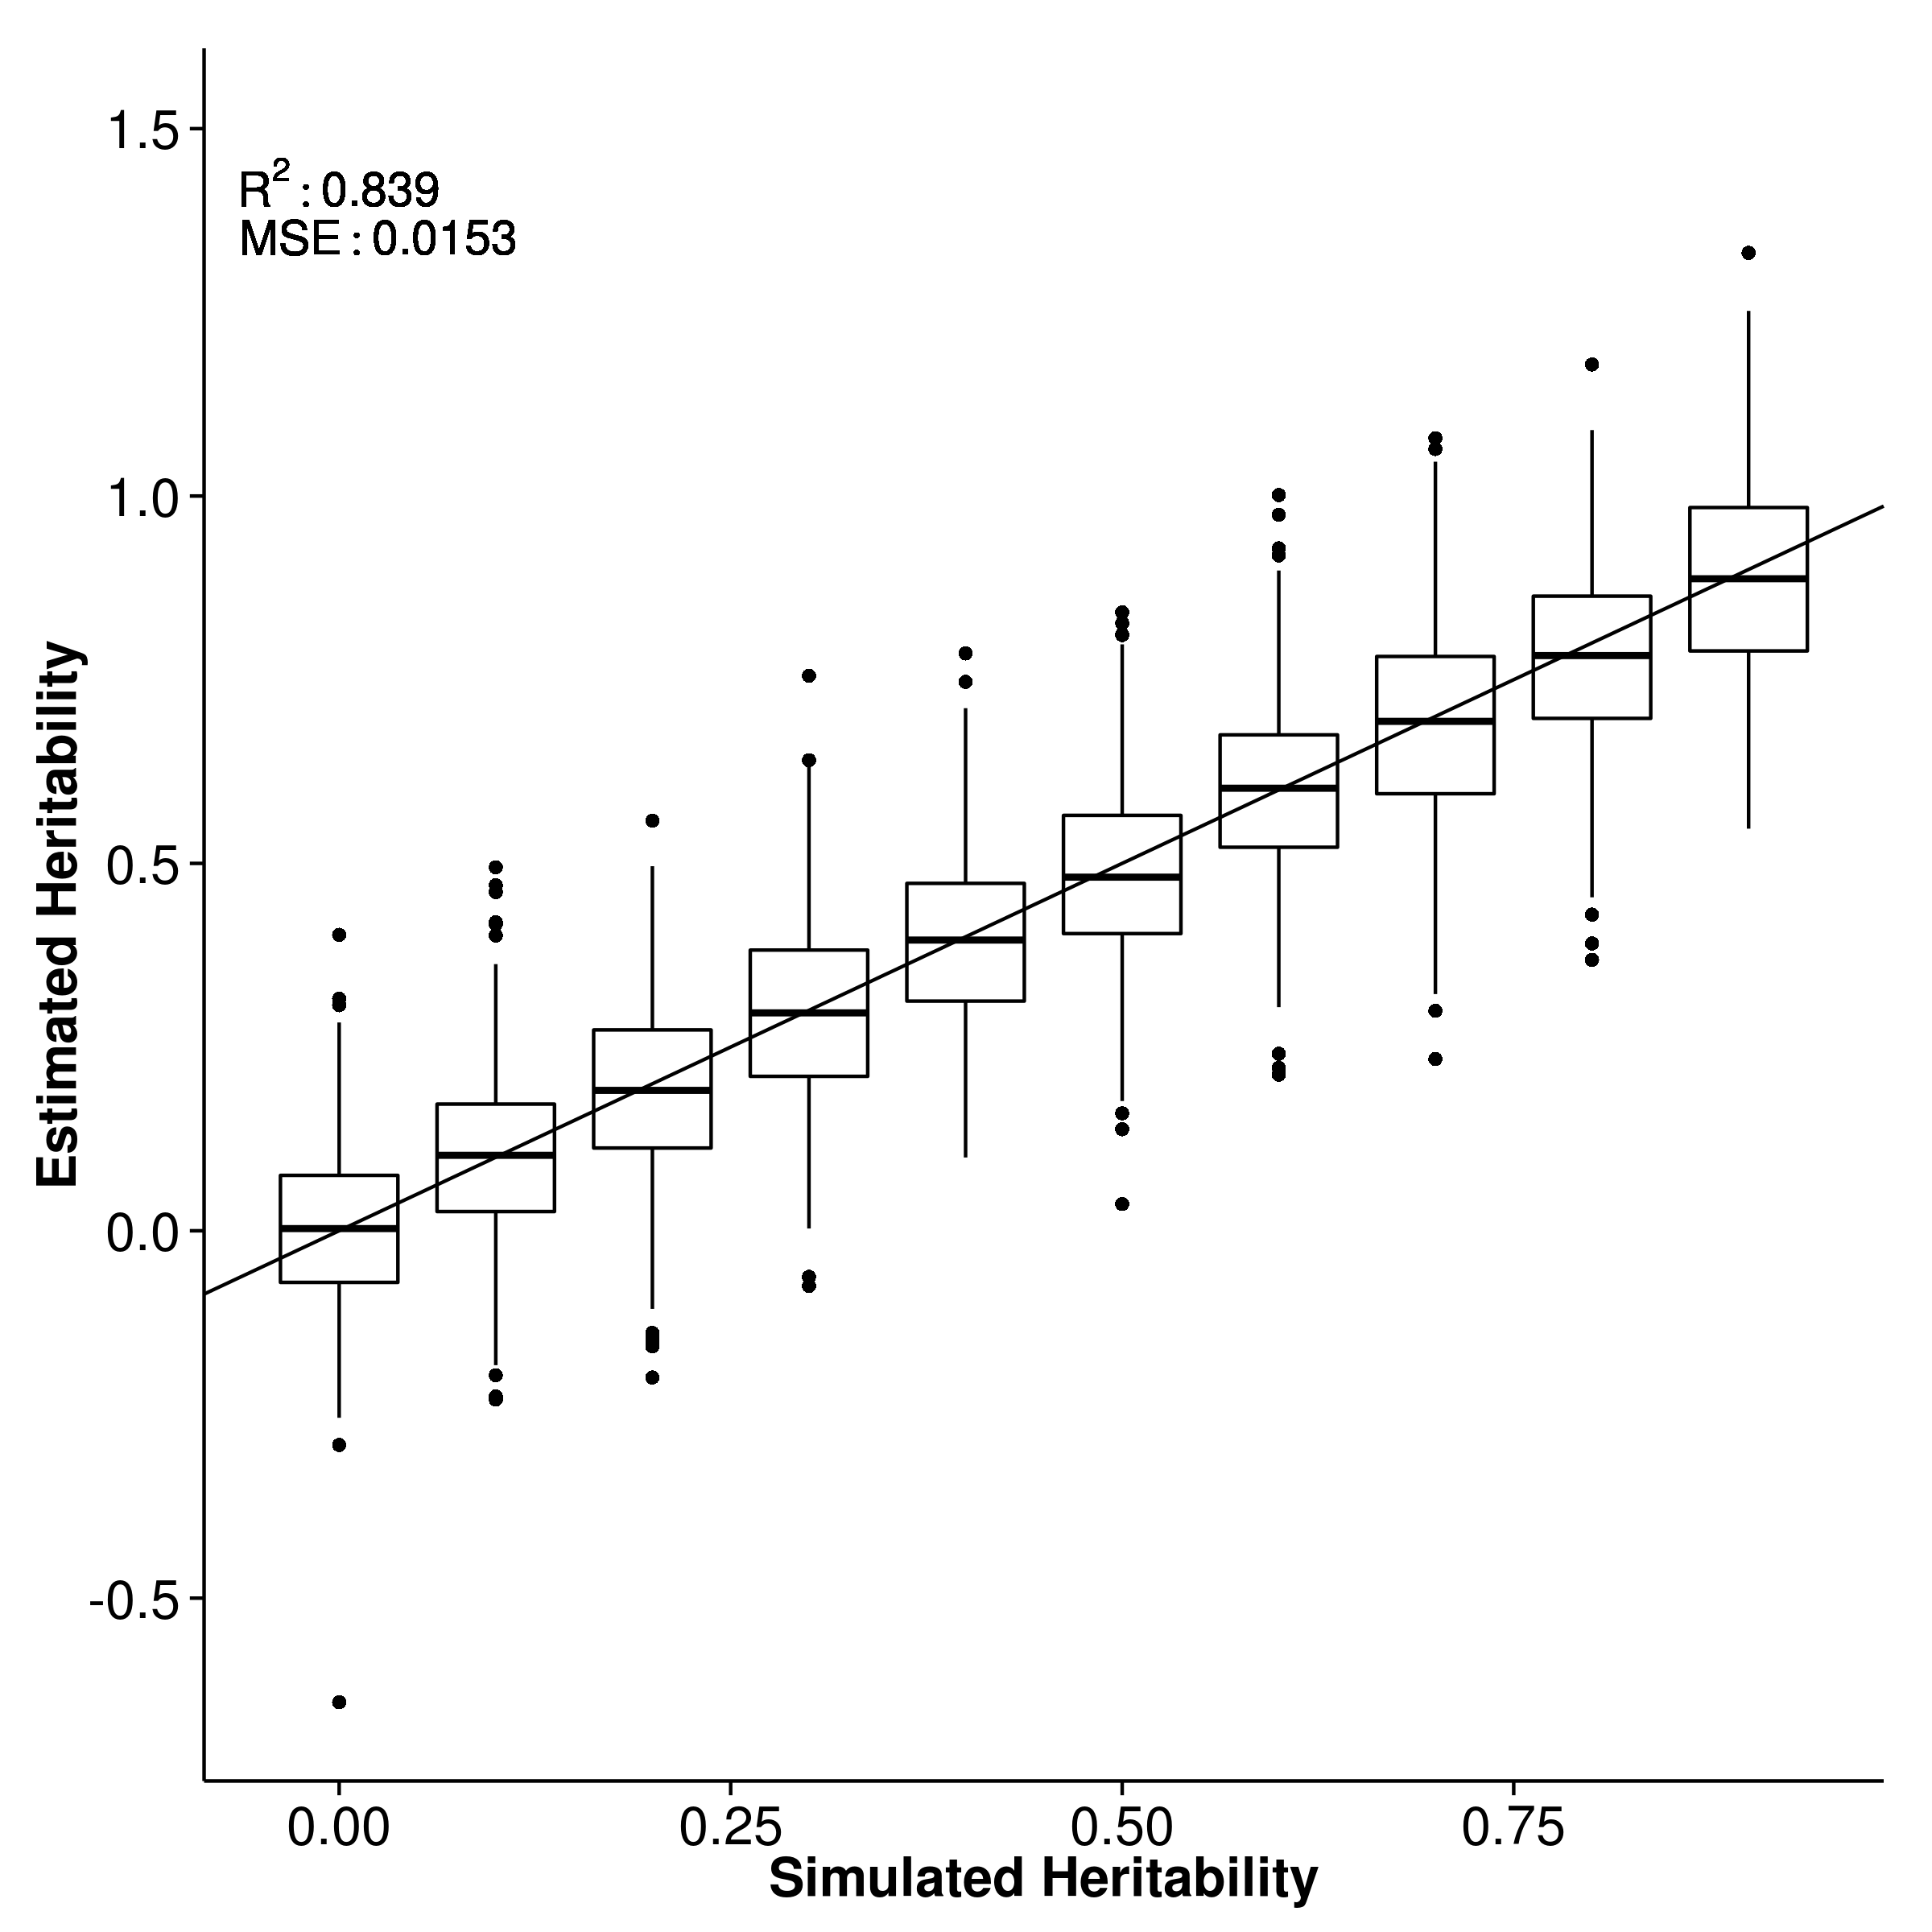
\includegraphics{figure/quantitative/random_effect/50c/shrek_50k_50c_meanH.png}}
			\label{fig:50k50cQtmeanSre}
		}
		\subfloat[GCTA]{
			\scalebox{.4}{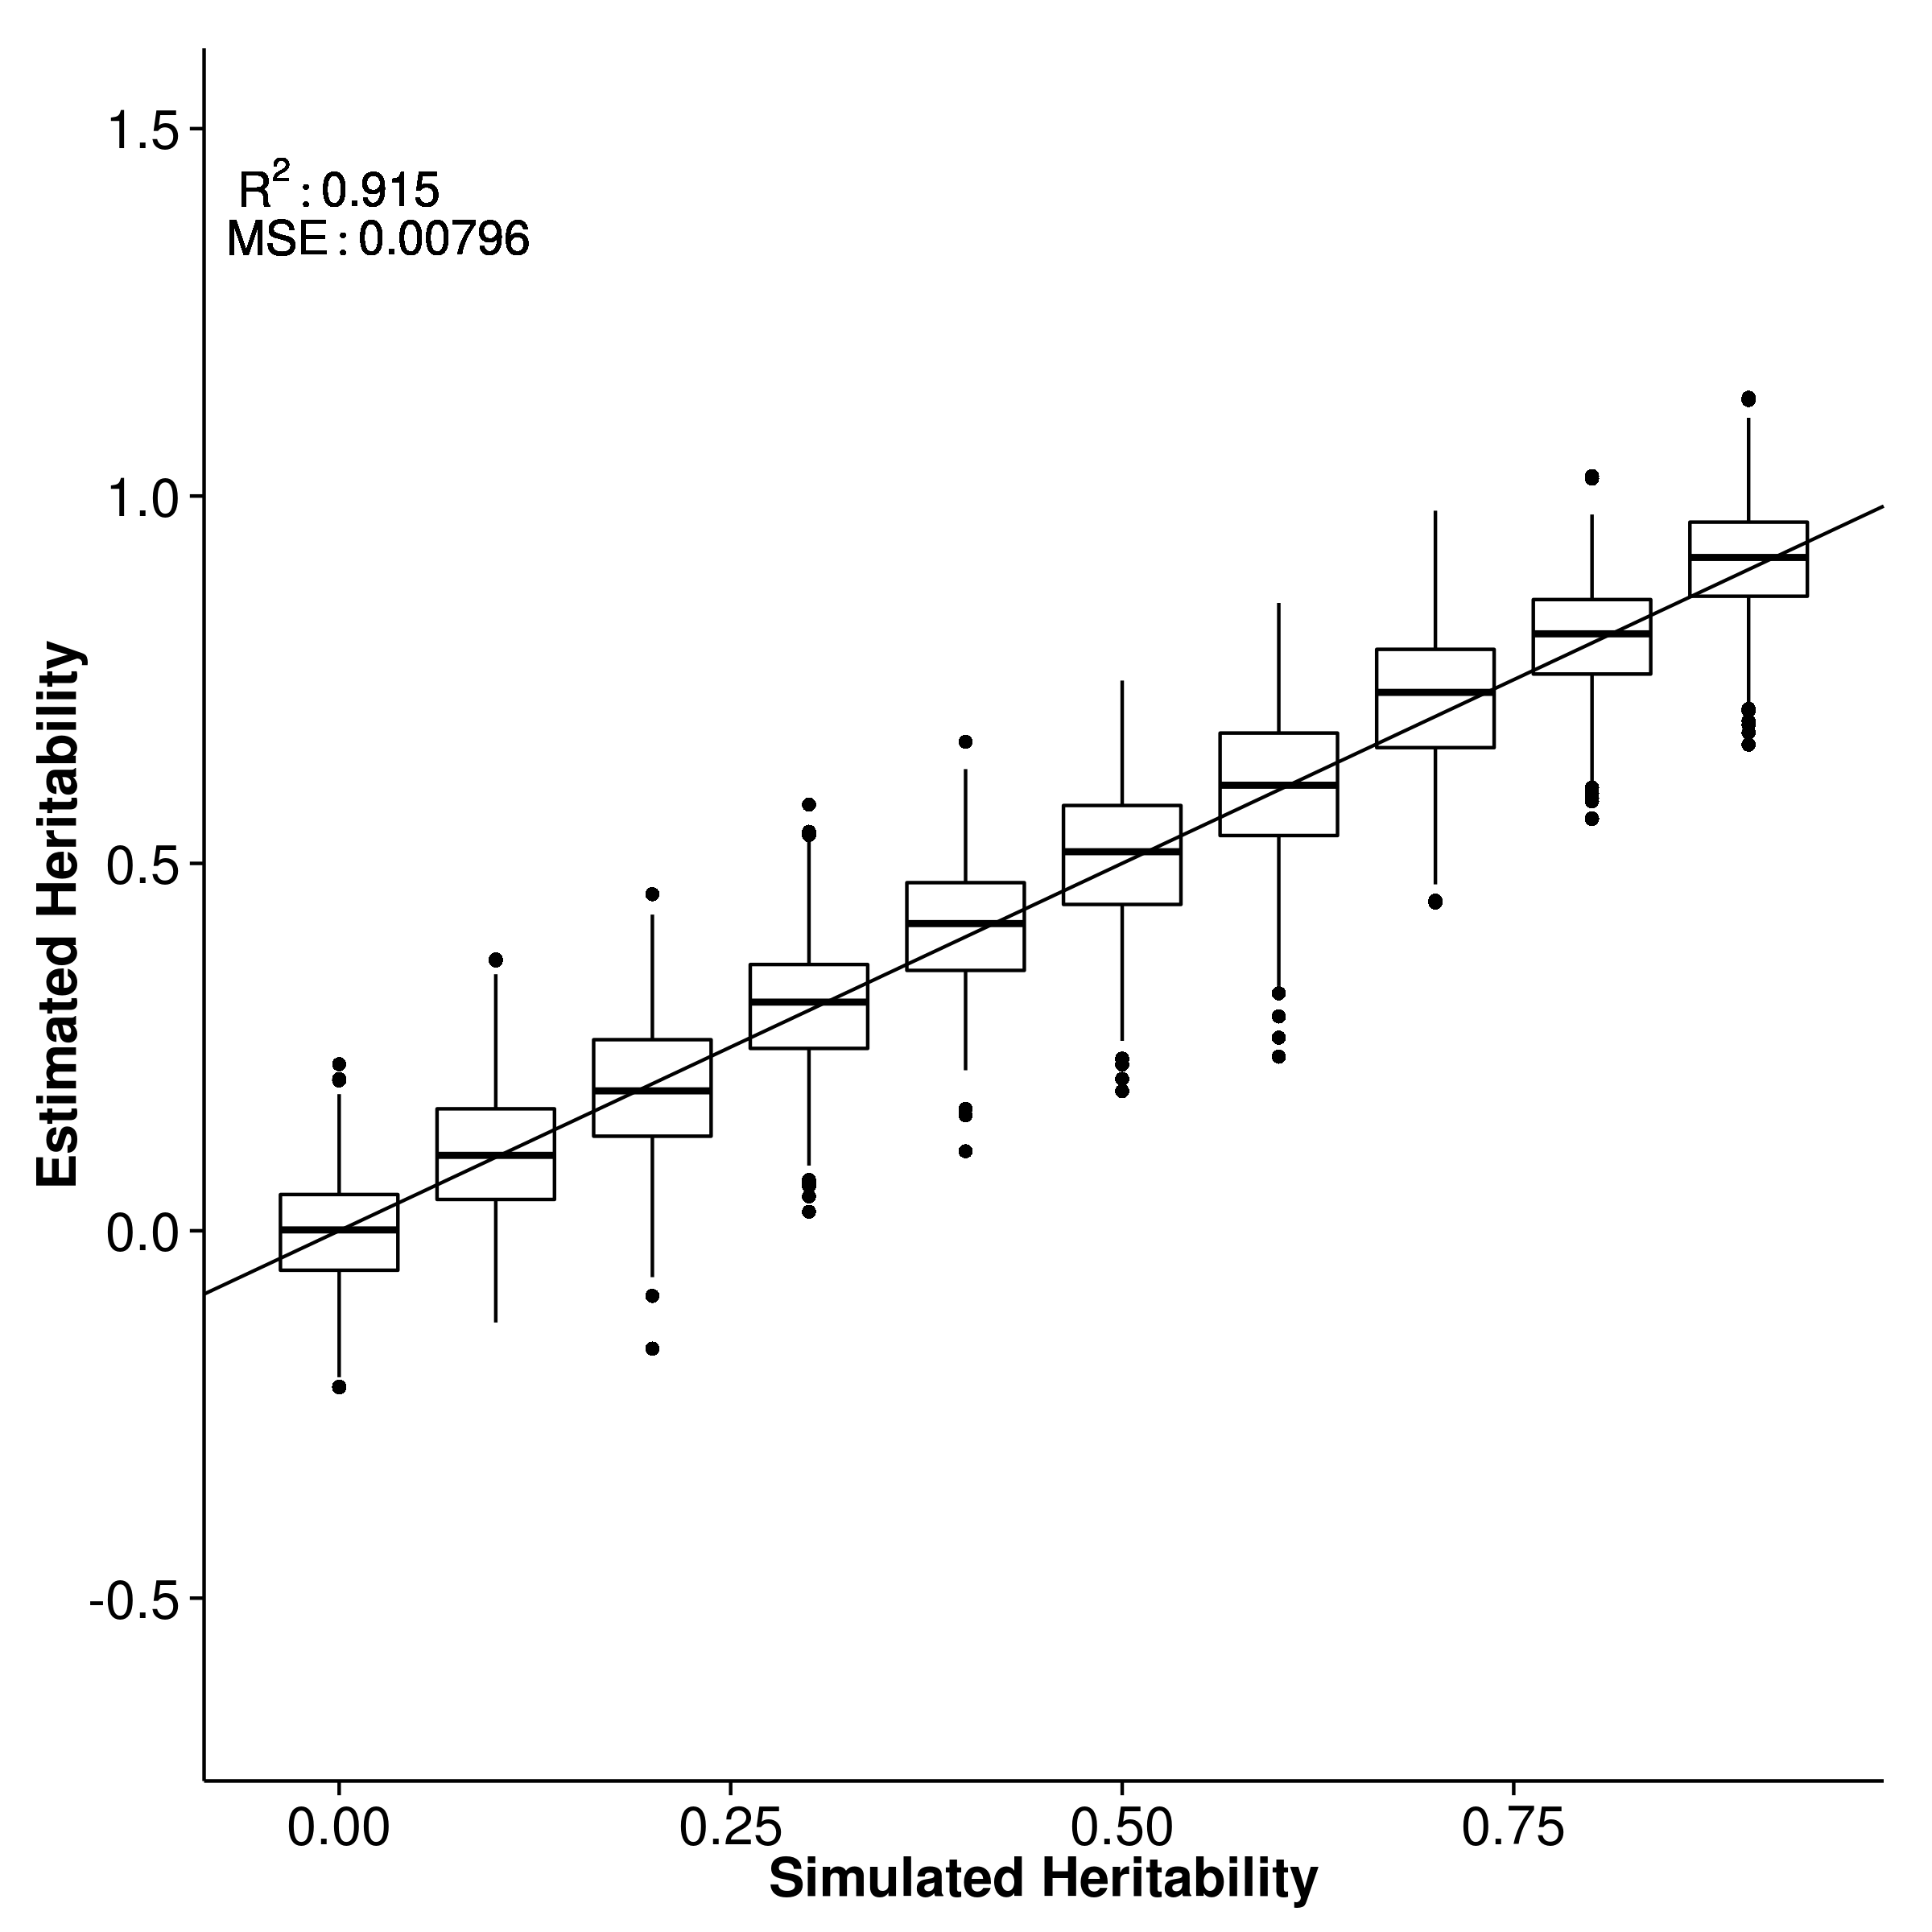
\includegraphics{figure/quantitative/random_effect/50c/gcta_50k_50c_meanH.png}}
			\label{fig:50k50cQtmeanGre}
		}\\
		\subfloat[LDSC with fix intercept]{
			\scalebox{.4}{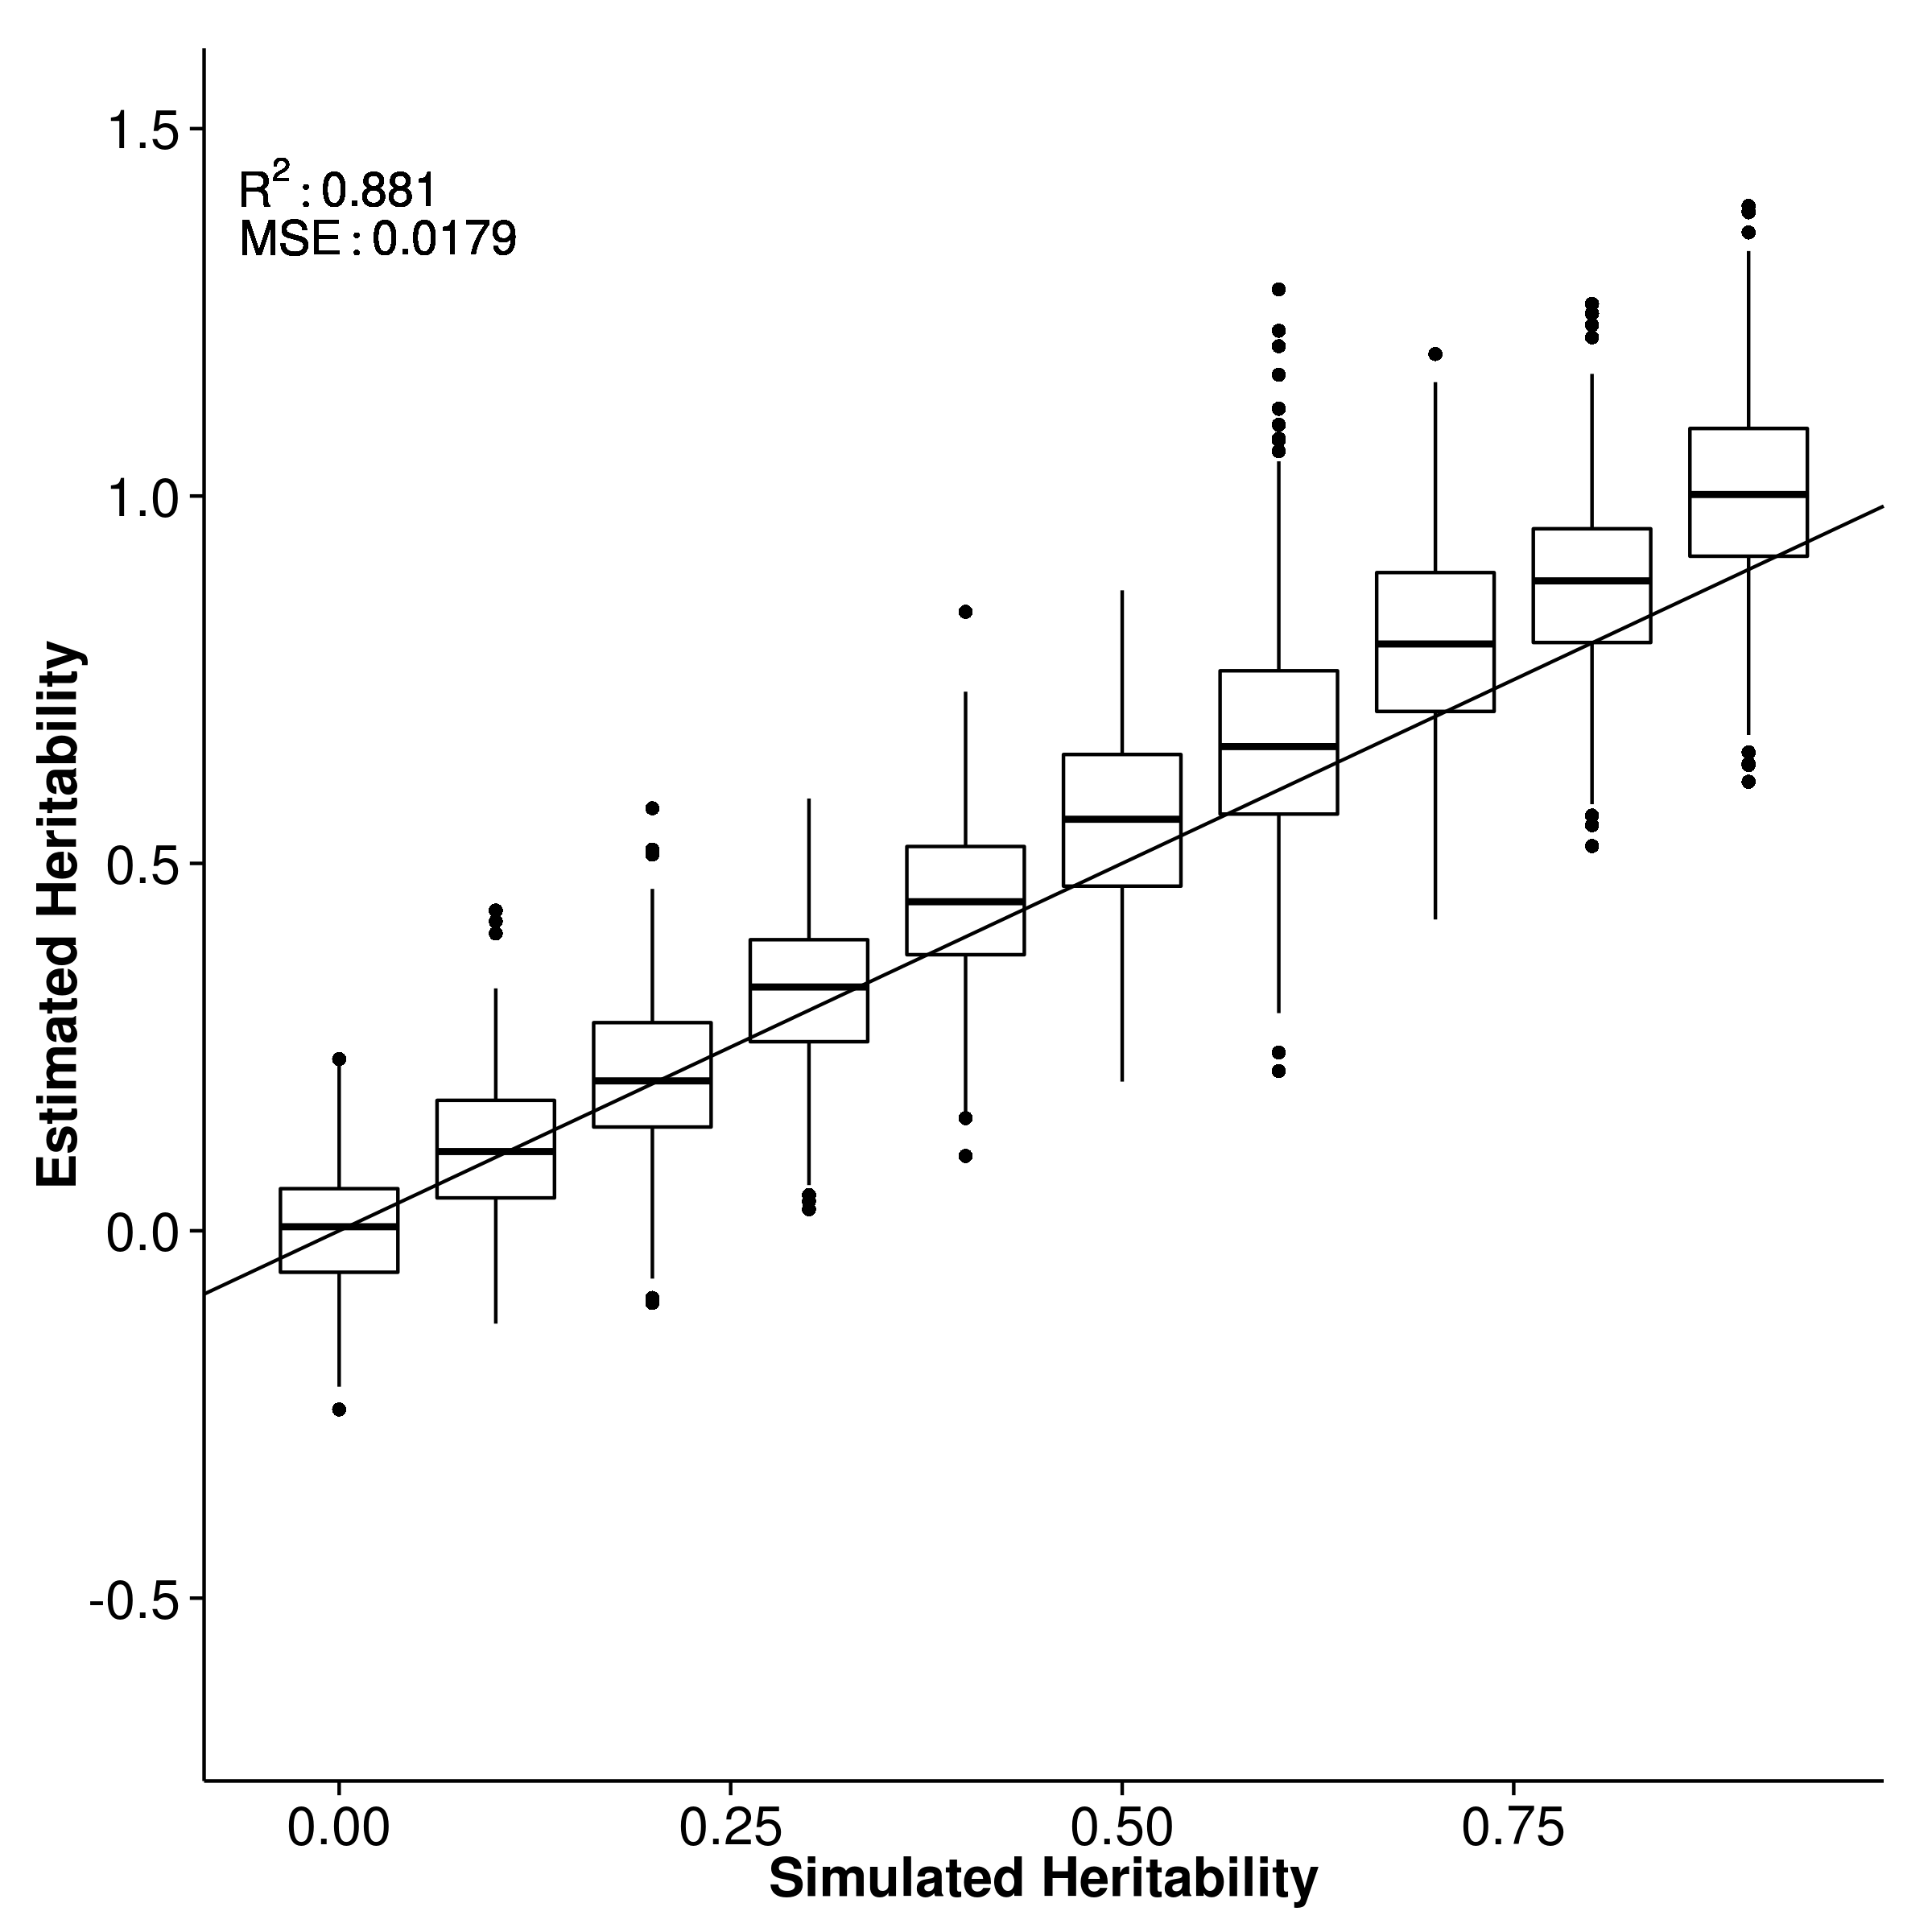
\includegraphics{figure/quantitative/random_effect/50c/ldsc_50k_50c_meanH.png}}
			\label{fig:50k50cQtmeanLre}
		}
		\subfloat[LDSC with intercept estimation]{
			\scalebox{.4}{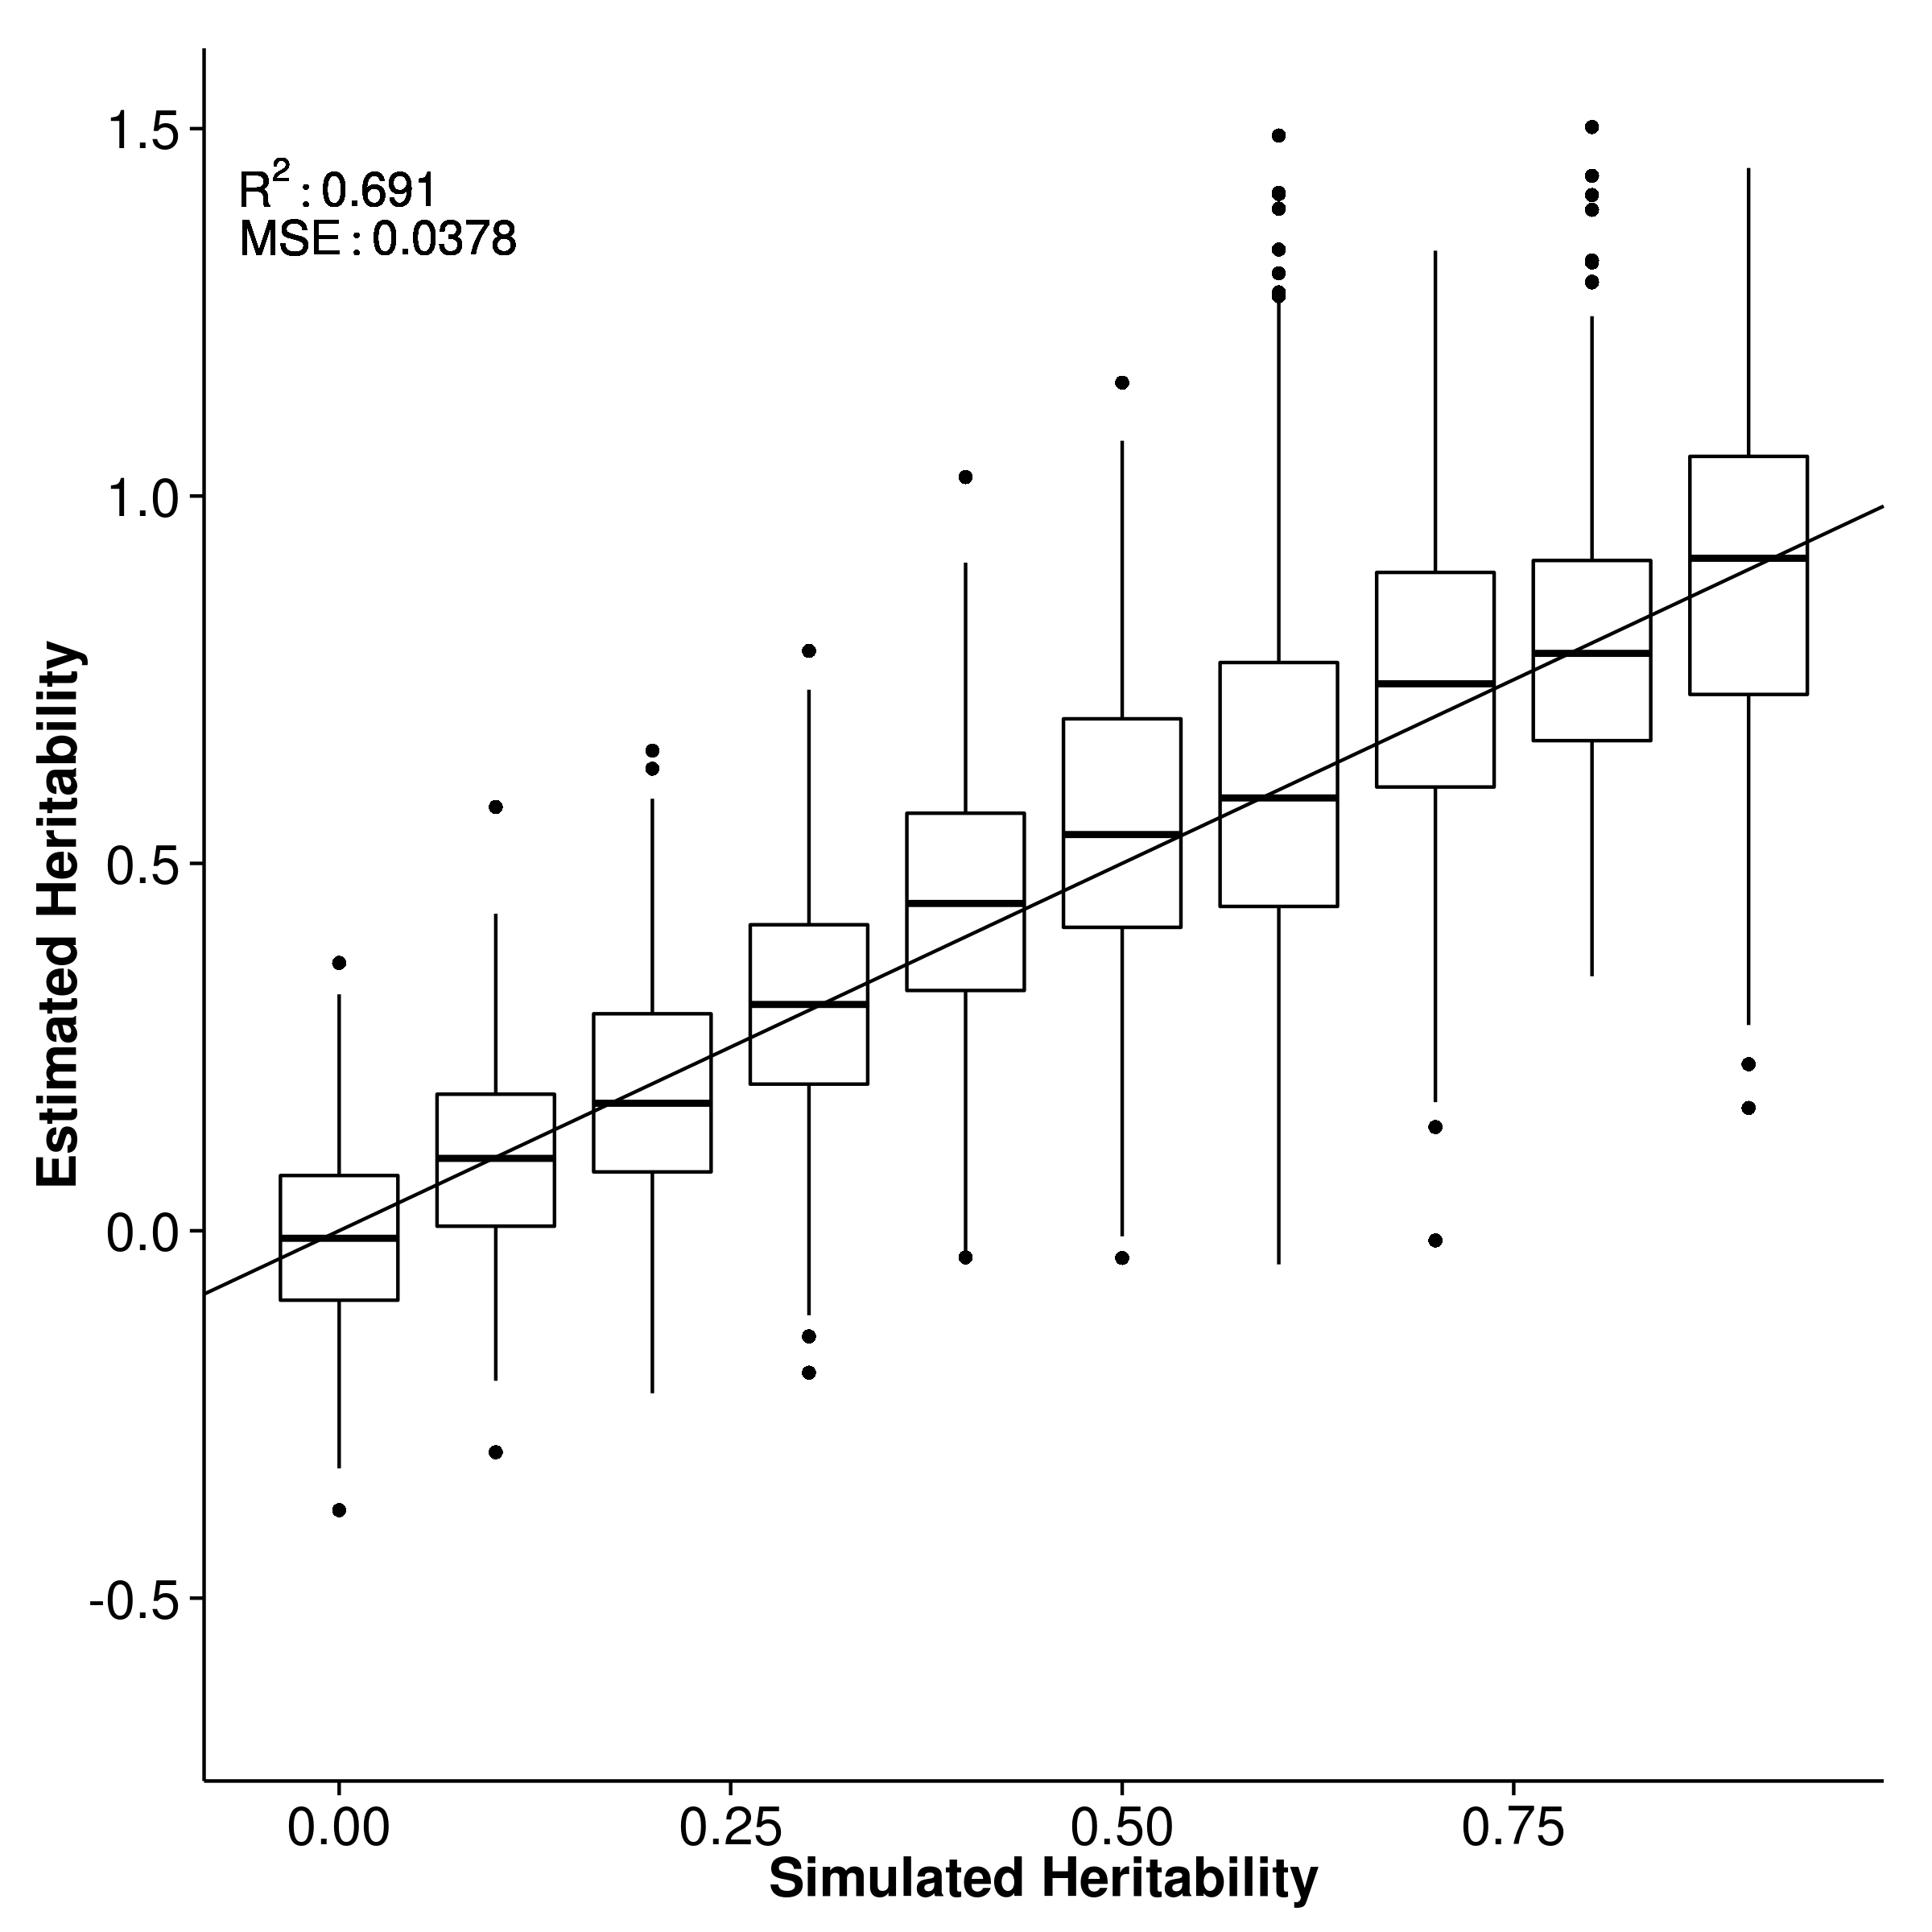
\includegraphics{figure/quantitative/random_effect/50c/ldscIn_50k_50c_meanH.png}}
			\label{fig:50k50cQtmeanIre}
		}
		\caption[Simulation of Quantitative Traits with 50k \glsentryshortpl{SNP} and 50 causal variants of random effect size]
		{Simulation of Quantitative Traits with 50k \glsentryshortpl{SNP} and 50 causal variants with random effect size.} 
		\label{fig:50k50cQtMeanre}
	\end{figure}
	\begin{figure}
		\centering
		\centering
		\subfloat[SHREK]{
			\scalebox{.4}{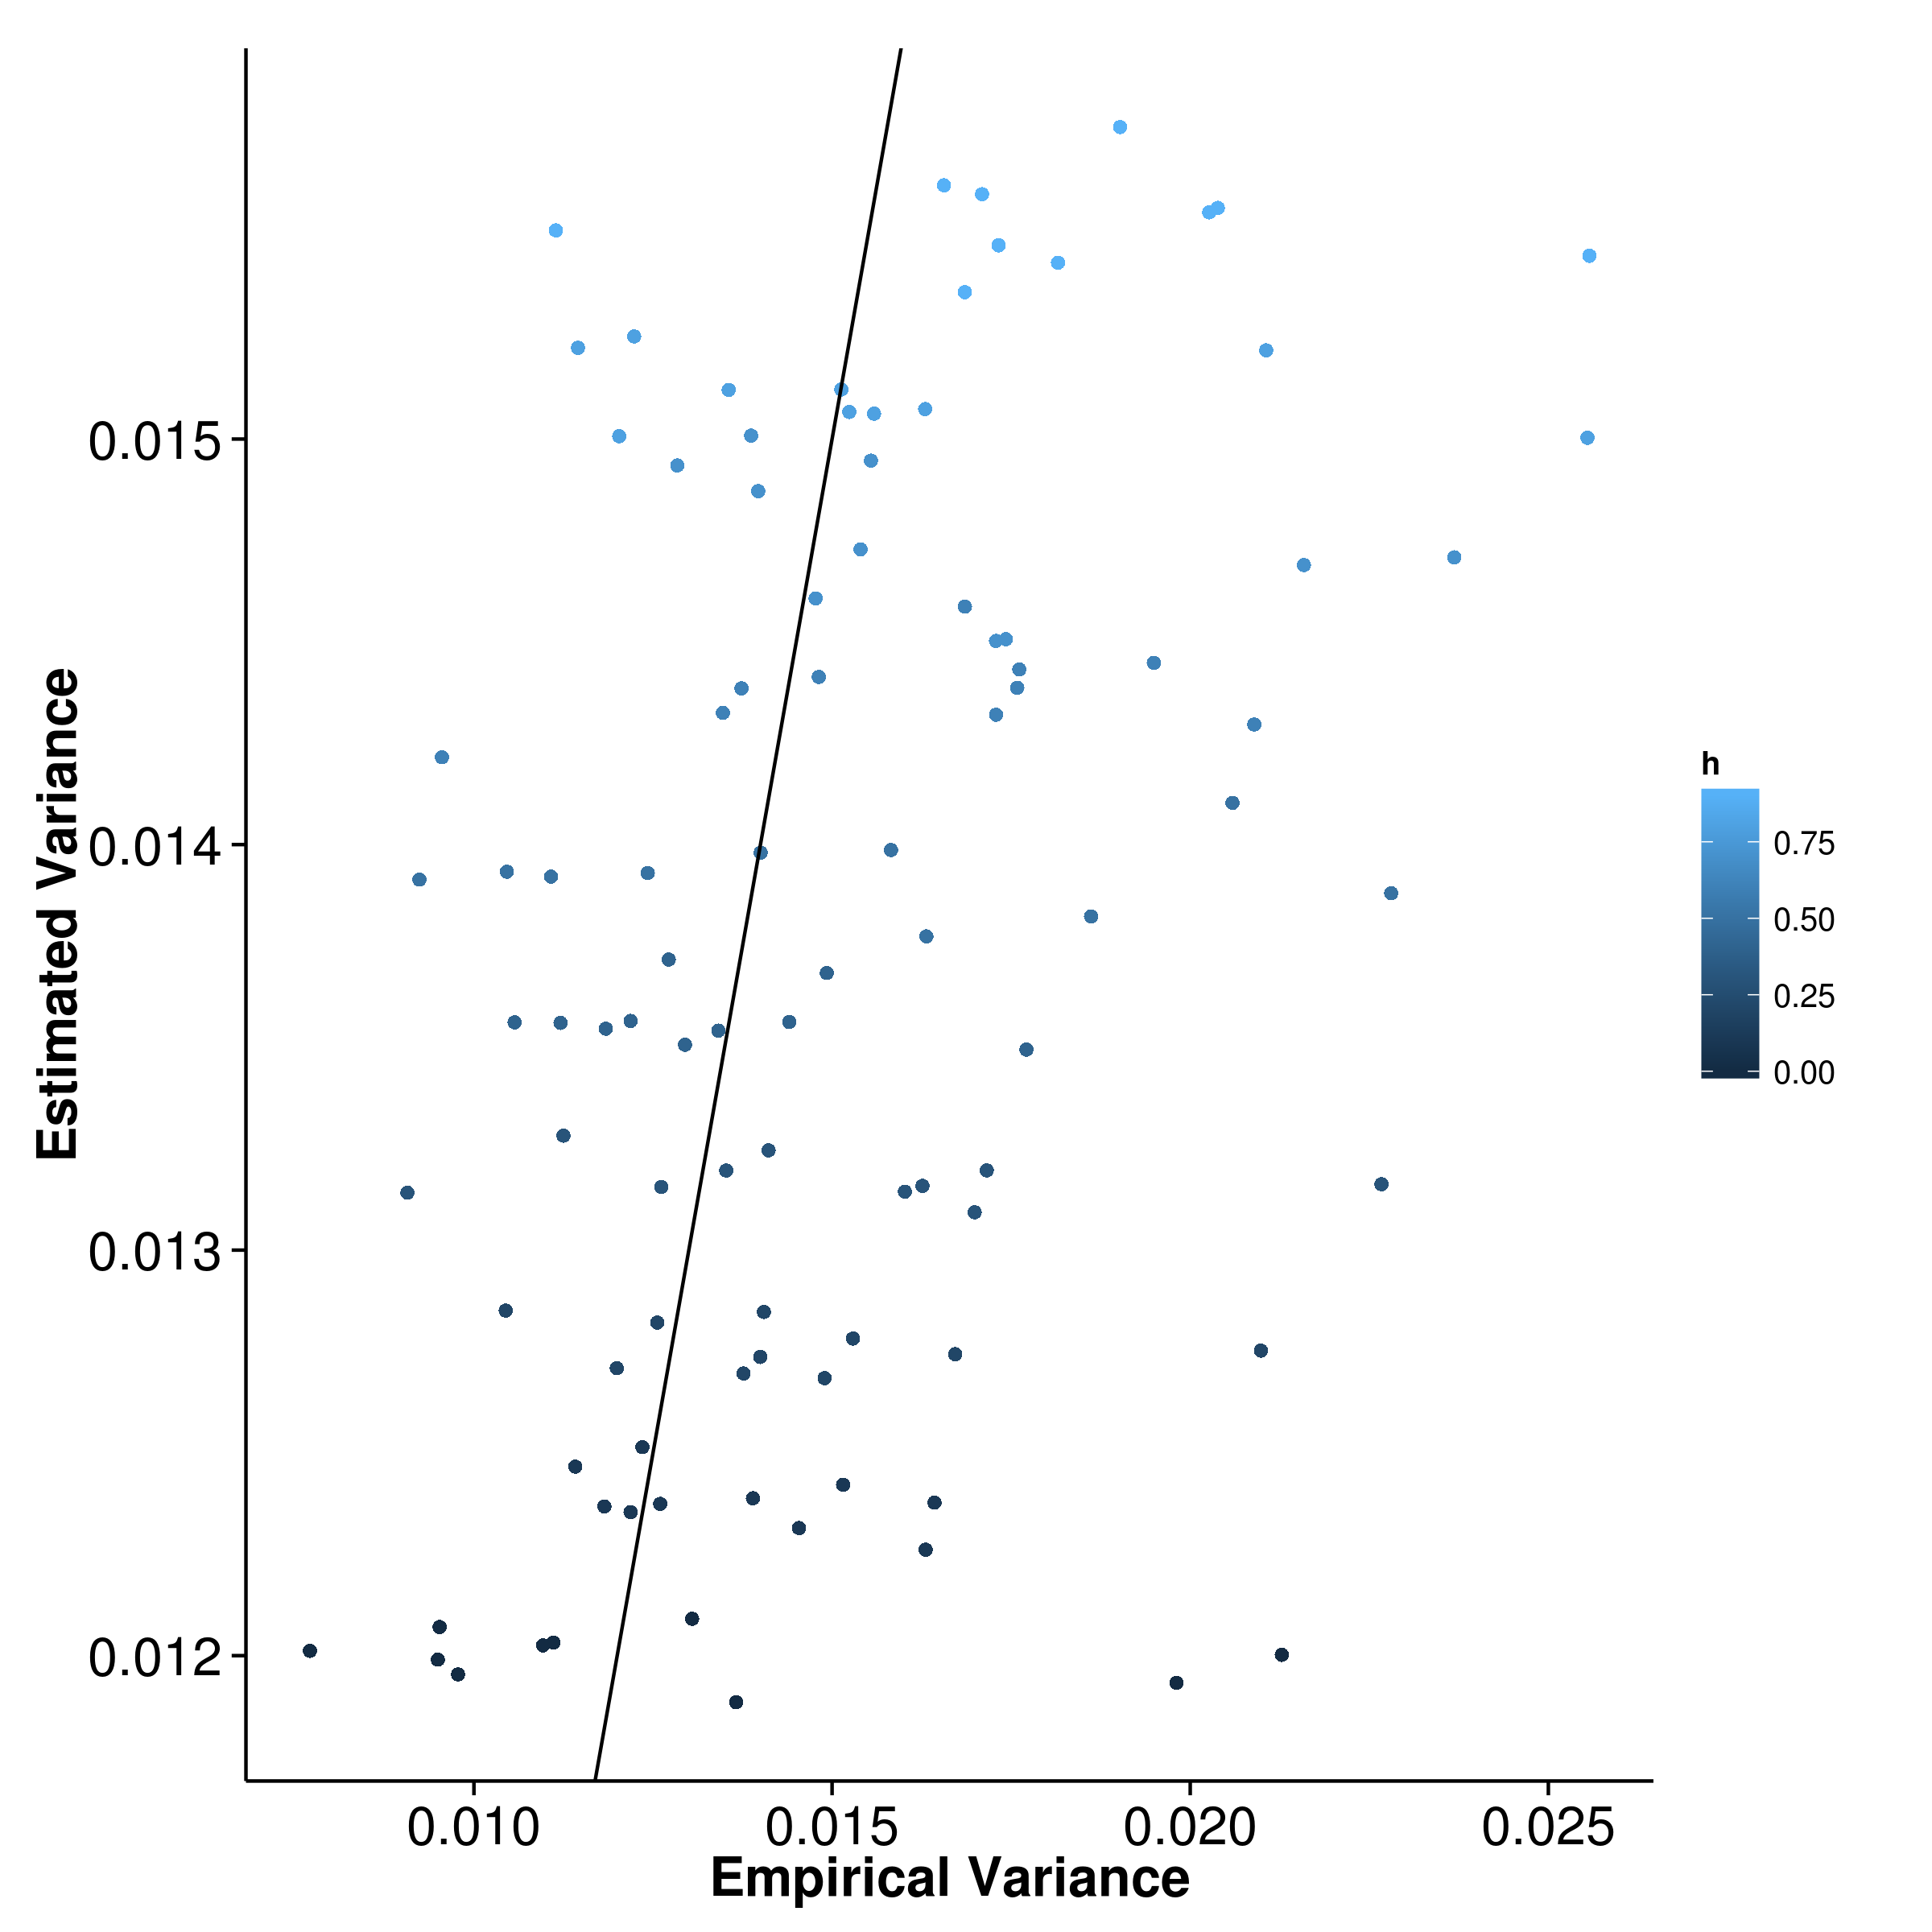
\includegraphics{figure/quantitative/random_effect/50c/shrek_50k_50c_varH.png}}
			\label{fig:50k50cQtvarSre}
		}
		\subfloat[GCTA]{
			\scalebox{.4}{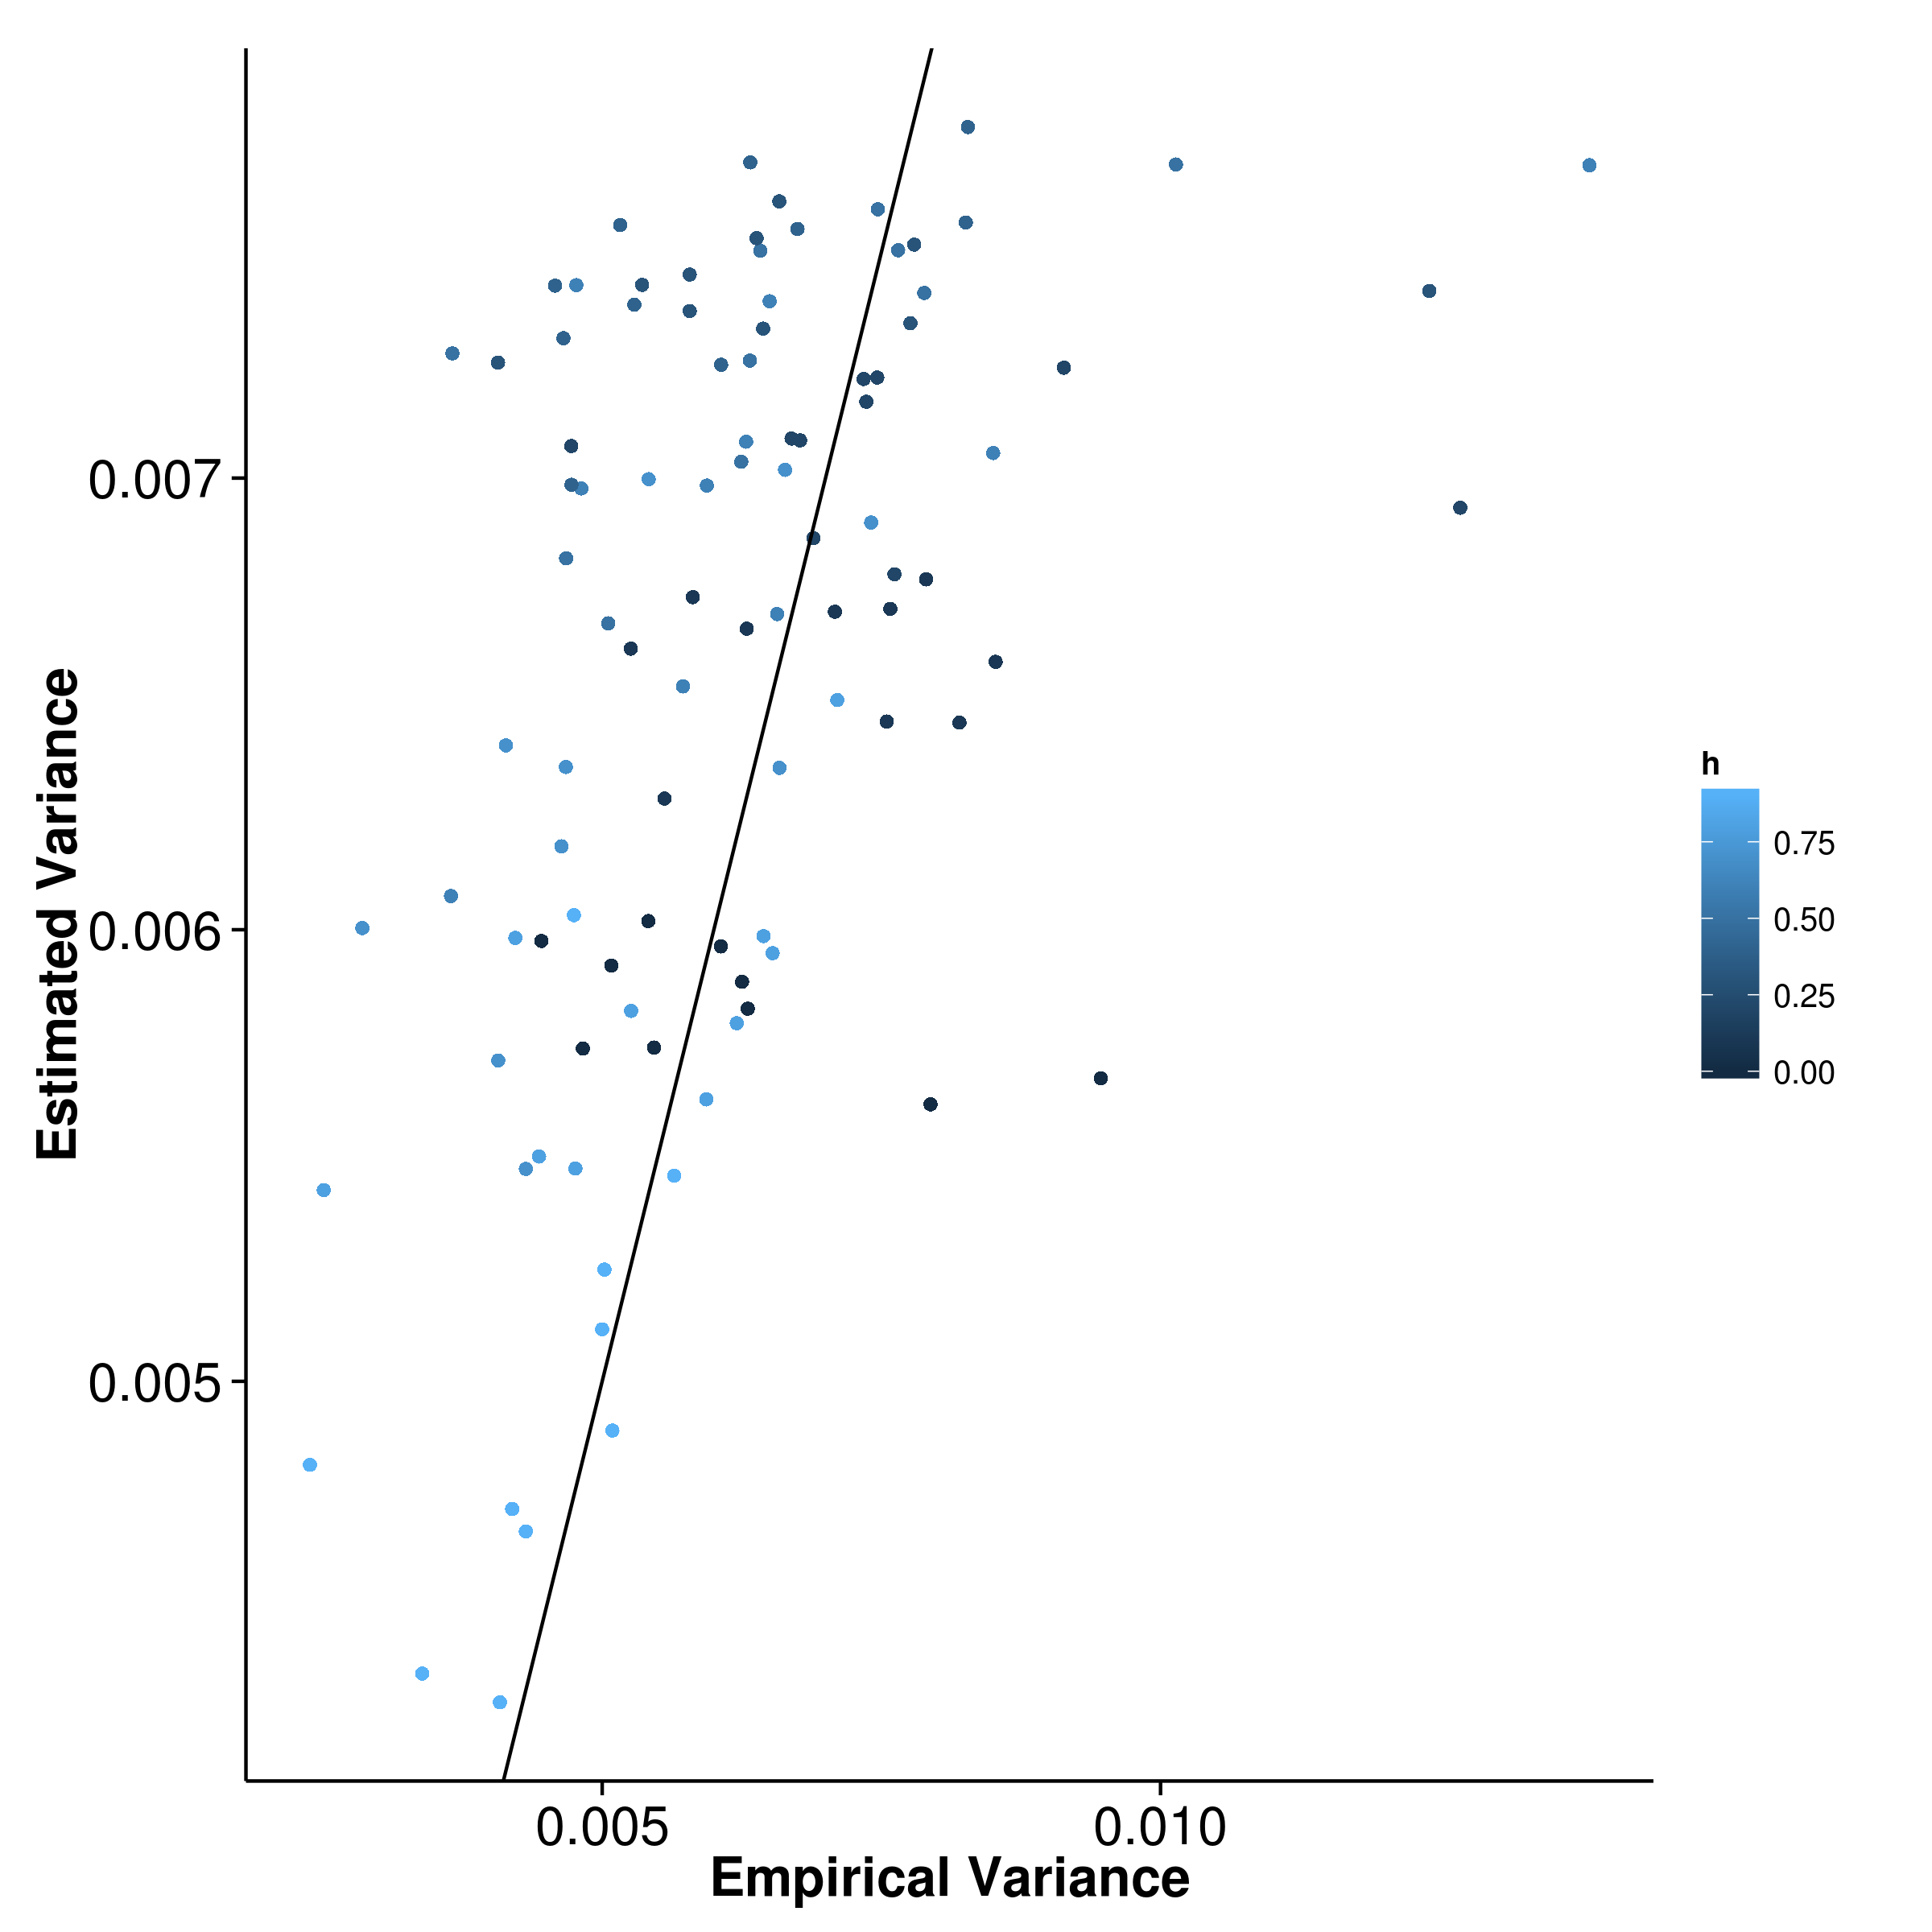
\includegraphics{figure/quantitative/random_effect/50c/gcta_50k_50c_varH.png}}
			\label{fig:50k50cQtvarGre}
		}\\
		\subfloat[LDSC with fix intercept]{
			\scalebox{.4}{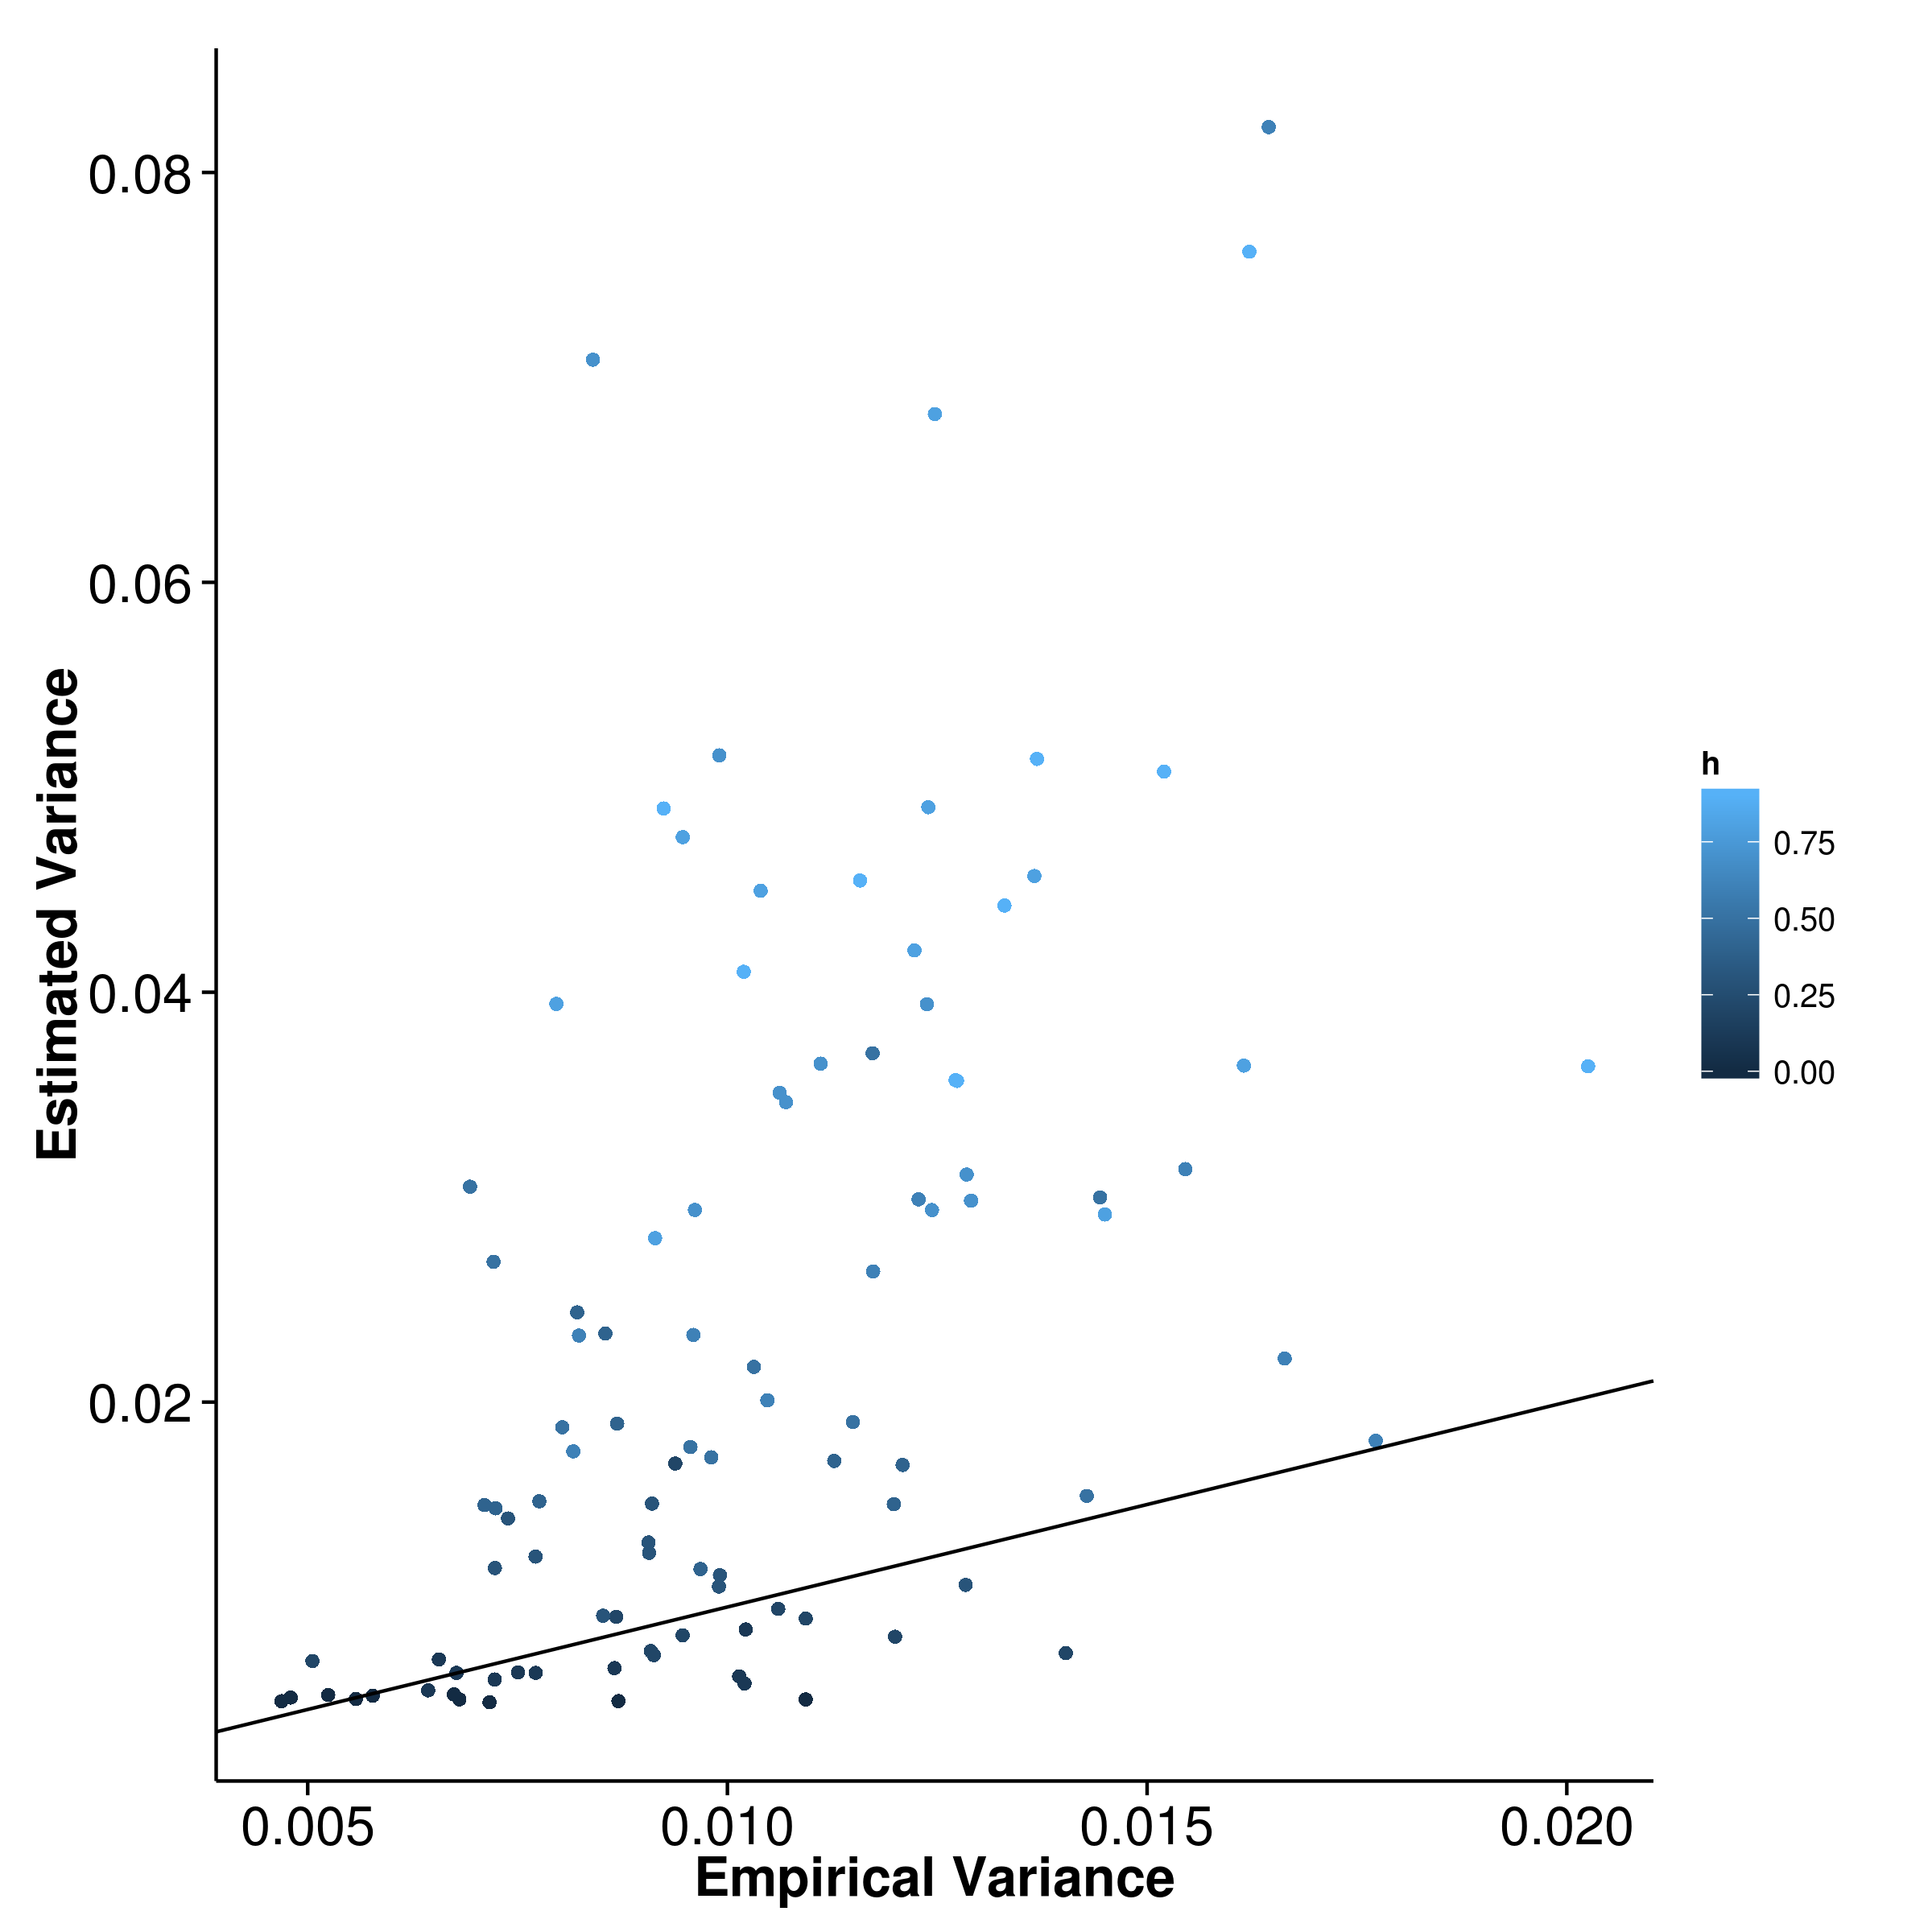
\includegraphics{figure/quantitative/random_effect/50c/ldsc_50k_50c_varH.png}}
			\label{fig:50k50cQtvarLre}
		}
		\subfloat[LDSC with intercept estimation]{
			\scalebox{.4}{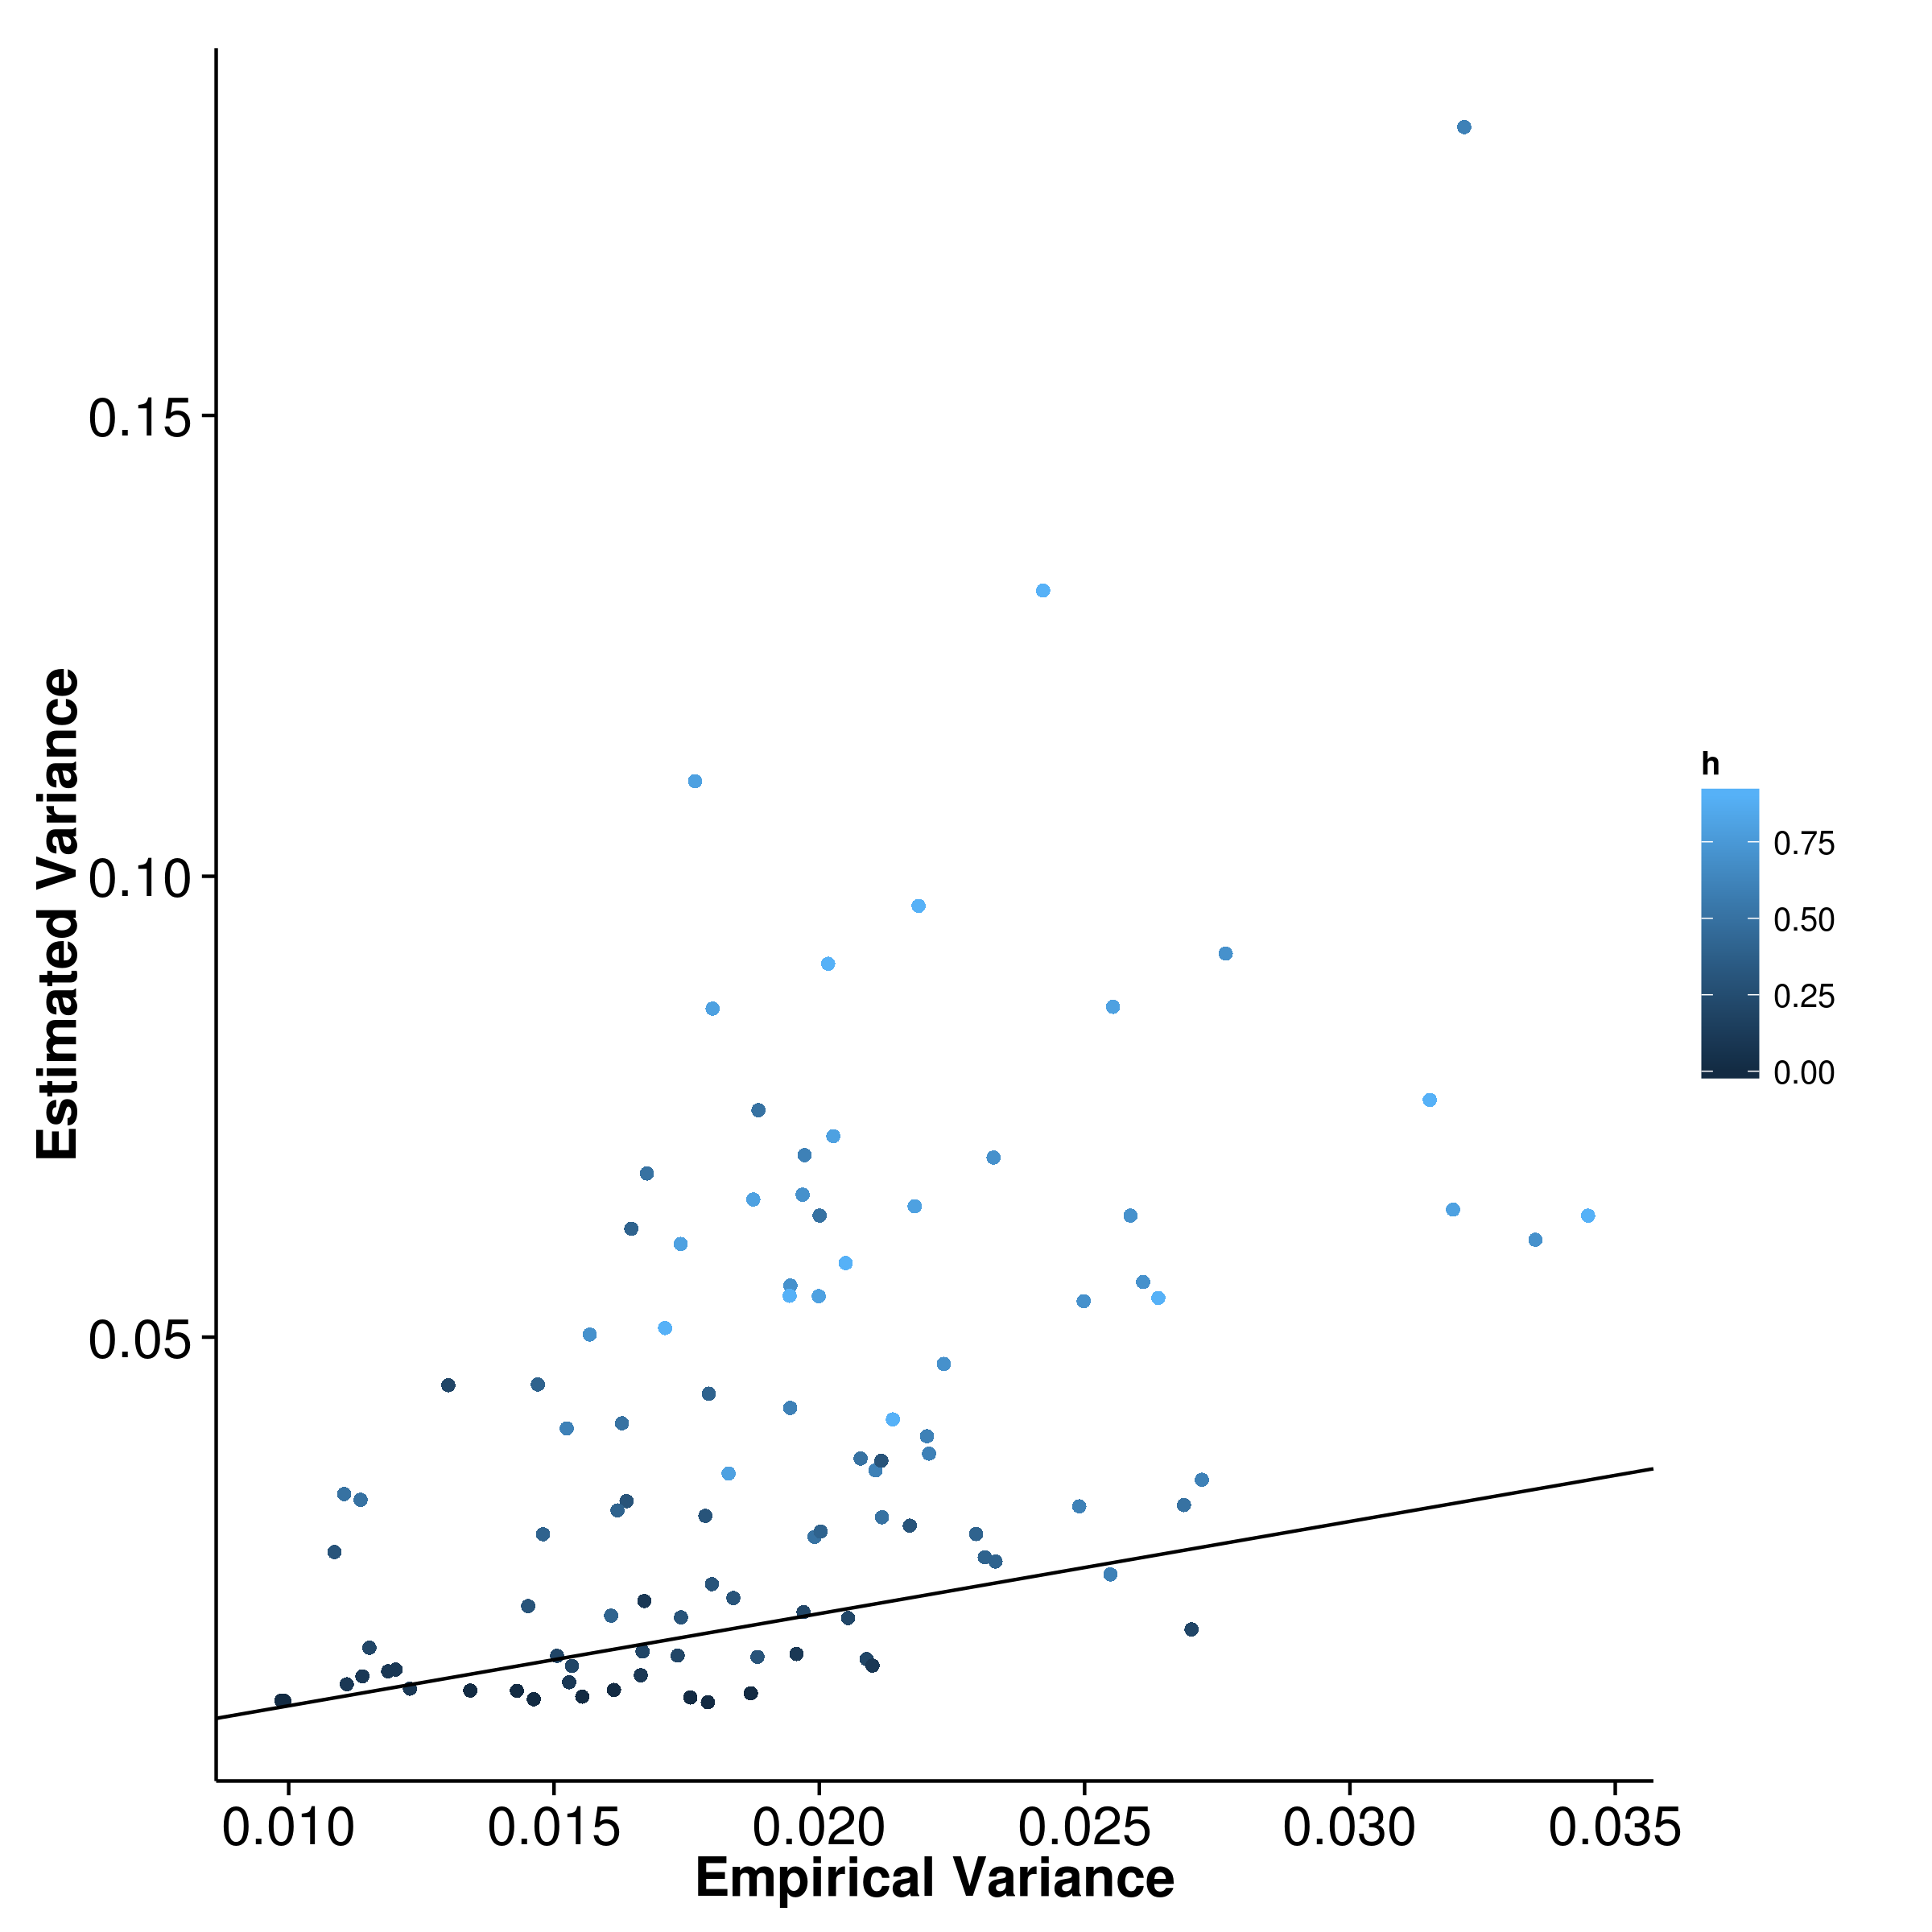
\includegraphics{figure/quantitative/random_effect/50c/ldscIn_50k_50c_varH.png}}
			\label{fig:50k50cQtvarIre}
		}
		\label{fig:50k50cQtVarre}
	\end{figure}